\documentclass[book,openany,lualatex,paper={182mm,232mm},fontsize=10pt,line_length=41zw,number_of_lines=33]{jlreq}
% 基本的な数学パッケージ
\usepackage{amsmath,amssymb}

% ブラケット記法 (\bra, \ket, \braket 等) を直感的に書くためのパッケージ
\usepackage{physics}

% 太字ベクトル用
\usepackage{bm}

% 虚数単位、自然対数の底、微分記号を立体にする
\newcommand{\ii}{\mathrm{i}}
\newcommand{\ee}{\mathrm{e}}
\RenewDocumentCommand{\dd}{}{\mathrm{d}}

% 量子回路図描画用パッケージ
\usepackage{graphicx} % \resizebox などで使用
\usepackage{tikz}
\usetikzlibrary{quantikz2} % 最新環境ではquantikz2が推奨されます
% 格子配置図・時空図・ブロック図で使う TikZ ライブラリ
\usetikzlibrary{positioning,calc,arrows.meta,fit,backgrounds,patterns,decorations.pathreplacing,shapes.geometric,3d}
% 図版の共通スタイル
\tikzset{
  xtype/.style={red!70!black},          % X 型（primal）
  ztype/.style={blue!70!black},         % Z 型（dual）
  ytype/.style={green!50!black},        % Y 型
  dataqubit/.style={circle, draw, fill=white, minimum size=4pt, inner sep=0pt},
  ancqubit/.style={circle, draw, fill=black!45, minimum size=4pt, inner sep=0pt},
  logpatch/.style={draw, dashed, thick}, % 論理アンシラパッチ
  xplaq/.style={fill=red!12, draw=red!70!black},
  zplaq/.style={fill=blue!12, draw=blue!70!black},
}

% ハイパーリンクの設定
\usepackage{xurl}
\usepackage[unicode,hidelinks]{hyperref}

% 長いコードパスを行末で安全に折り返す
\newcommand{\codepath}[1]{\nolinkurl{#1}}
\newcommand{\codeinline}[1]{\nolinkurl{#1}}

% 長い日本語文とインラインコードが混在する段落の微小なはみ出しを防ぐ
\setlength{\emergencystretch}{2em}

% 本文幅に追従する比較表
\usepackage{tabularx}

% ソースコード表示用の設定 (Python/Qiskit等を想定)
\usepackage{listings}
\usepackage{xcolor}
% listingsのLOL出力を無効化（\@writefileのバッファ問題回避）
\makeatletter
\AtBeginDocument{\renewcommand{\lstlistoflistings}{}}
\AtEndDocument{%
  \let\orig@end@writefile\@writefile
  \renewcommand{\@writefile}[2]{%
    \def\@end@tmp@ext{lol}%
    \def\@end@tmp@arg{#1}%
    \ifx\@end@tmp@ext\@end@tmp@arg
    \else
      \orig@end@writefile{#1}{#2}%
    \fi
  }%
}
\makeatother

% コールアウト用ボックス
\usepackage{tcolorbox}
\tcbuselibrary{breakable}

% チャプターゴール / Note / 警告 / 演習 環境
\newtcolorbox{chaptergoal}{
  colback=blue!5,
  colframe=blue!60!black,
  title=\textbf{この章で学ぶこと},
  fonttitle=\bfseries,
  breakable
}
\newcommand{\cgitem}{\textbullet\ }

\newtcolorbox{notebox}{
  colback=blue!5,
  colframe=blue!60!black,
  title=\textbf{Note},
  fonttitle=\bfseries,
  breakable
}

\newtcolorbox{warningbox}{
  colback=yellow!5,
  colframe=orange,
  title=\textbf{注意},
  fonttitle=\bfseries,
  breakable
}

\newtcolorbox{exercise}[1][演習]{
  colback=green!5,
  colframe=green!50!black,
  title=\textbf{#1},
  fonttitle=\bfseries,
  breakable
}

\lstset{
    language=Python,
    basicstyle=\ttfamily\small,
    keywordstyle=\color{blue}\bfseries,
    stringstyle=\color{red},
    commentstyle=\color{green!50!black},
    numbers=left,
    numberstyle=\tiny\color{gray},
    stepnumber=1,
    numbersep=5pt,
    backgroundcolor=\color{black!5},
    frame=single,
    rulecolor=\color{black!20},
    breaklines=true,
    tabsize=4,
    captionpos=b,
    showstringspaces=false
}


% openany でも jlreq は部扉の前を奇数ページまで送り、\frontmatter/\mainmatter で
% \cleardoublepage するため空白ページが残る。画面で読む前提なので改ページのみにする。
% （印刷に回す場合は openany とあわせてこのブロックを外す）
\makeatletter
\renewcommand{\jlreq@cleartooddpage}[1][]{\clearpage}
\makeatother
\jlreqsetup{frontmatter_pagebreak=clearpage,mainmatter_pagebreak=clearpage}

\title{ゼロから作る FTQC シミュレータ\\— Stim で学ぶ誤り耐性量子計算の実装}
\author{森 俊夫}
\date{\today}

\begin{document}

\hypersetup{pageanchor=false}
\maketitle

\frontmatter
\hypersetup{pageanchor=true}
\setcounter{tocdepth}{1} % 目次は節（\section）まで表示する
\tableofcontents

\chapter*{まえがき}
\addcontentsline{toc}{chapter}{まえがき}
本書では、Stim を用いた誤り耐性量子計算（FTQC）の小さなシミュレータを、基礎から段階的に組み立てます。安定化器回路、表面符号、格子手術を学び、最後に回路レベルの誤りと論理状態のトラジェクトリを結び付けます。各段階では、実装が何をモデル化し、どの検査で確かめられるかを区別します。シミュレーション結果は、明示した物理・論理モデルの範囲で解釈してください。

本書は第I部から第V部までで構成します。前半では量子誤り訂正と Stim の基礎を学び、Stage 01 の現象論的 MPP モデル、Stage 02 の回路レベルモデル、Stage 03 の統合ランタイムへ進みます。第25章で扱うのは $d=3$ 固定の実装です。距離一般化や、完全な相関付き論理パウリフレームは本書の範囲外です。

本文のコードは、本書に同梱した独立実行環境に対応します。Stage 01 と Stage 02 はそれぞれ専用のソース、テスト、例、依存関係を持ちます。Stage 03 はリポジトリ直下の \codepath{src/ftqc}、\codepath{tests}、\codepath{examples}、\codepath{pyproject.toml} を使います。環境構築と実行方法は付録A、構成は付録B、検証の解釈と制限は付録C、引用文献は付録Dを参照してください。

\mainmatter

% ----- 第I部 -----
\part{基礎 — なぜ FTQC シミュレータが必要か}\label{part:foundations}

% Stage: —（理論）／ 説明用コード: —
\chapter{量子コンピュータ概要}\label{ch:overview}

\begin{chaptergoal}
  \begin{itemize}
  \item 量子ビット・重ね合わせ・量子もつれ・測定という基本概念を整理します。
  \item 量子ゲートと量子回路の記法を確認し、後章で使う $H,S,T,\mathrm{CNOT}$ を押さえる。
  \item NISQ と FTQC のギャップを理解し、本書が作るハイブリッドシミュレータの位置づけを掴む。
  \end{itemize}
\end{chaptergoal}

本書は、Stim（高速スタビライザ／QEC サンプリング）と状態ベクトル（非クリフォード）、ソフトウェア上のフレーム追跡を組み合わせた\textbf{ハイブリッド型 FTQC シミュレータ}を、段階的にゼロから組み上げる実装書です。
その出発点として、本章では実装に必要な最小限の量子計算の基礎を整理します。
すでに量子計算の入門を終えている読者は、本章をざっと眺めて第2章へ進んでかまいません。

\begin{notebox}
  本章は理論の章です。実行コードは出さず、記法と語彙を揃えることに集中します。
  実装は第~II~部以降（まず Stim、続いて \codepath{src/stages/01_mpp/src/ftqc/} など）で扱います。
\end{notebox}

\section{量子ビット・重ね合わせ・量子もつれ・測定}\label{sec:qubit}

\subsection{古典ビットと量子ビット}

古典ビットは $0$ か $1$ のいずれか一方の値だけを持ちます。
これに対し\textbf{量子ビット}は、計算基底 $\ket{0},\ket{1}$ の\textbf{重ね合わせ}を許す二準位系です。
一般の純状態は
\begin{equation}
  \ket{\psi}
  = \alpha\ket{0} + \beta\ket{1},
  \qquad
  |\alpha|^2 + |\beta|^2 = 1
\end{equation}
と書けます。複素係数 $\alpha,\beta$ を\textbf{確率振幅}と呼びます。
全体にかかるグローバル位相 $\ee^{\ii\phi}$ は観測に影響しないため、状態は実質ブロッホ球上の一点として描けます（幾何の詳細は本書では深入りしません）。

\subsection{測定と射影}

計算基底での\textbf{測定}は、確率 $|\alpha|^2$ で結果 $0$、$|\beta|^2$ で結果 $1$ を返し、測定後の状態は対応する基底 $\ket{0}$ または $\ket{1}$ に\textbf{射影}されます。
つまり測定は重ね合わせを\textbf{壊します}。
古典情報のように「見ても壊さないコピー」が取れないことが、誤り訂正を古典とは根本的に変えます（第3章）。

\subsection{多量子ビットと量子もつれ}

$n$ 量子ビットの計算基底は $\ket{x}$（$x\in\{0,1\}^n$）で、$2^n$ 次元の複素ヒルベルト空間に住みます。
特に重要なのが、積状態 $\ket{\psi}\otimes\ket{\phi}$ に分解できない\textbf{量子もつれ}です。
代表例がベル状態
\begin{equation}
  \ket{\Phi^+}
  = \frac{1}{\sqrt{2}}\bigl(\ket{00}+\ket{11}\bigr)
\end{equation}
です。一方を測ると他方の結果が即座に確定しますが、情報は光速を超えて送れません。
格子手術や論理 CNOT の理解でも、「相関したパリティ」という形でもつれが現れます。

\begin{notebox}
  用語について。本書では entanglement を\textbf{量子もつれ}と呼びます。
  また量子ビット・重ね合わせなどの英語を括弧で繰り返すことはしません。
\end{notebox}

\section{量子ゲートと量子回路}\label{sec:gates}

量子計算の基本は、初期状態（多くは $\ket{0}^{\otimes n}$）に\textbf{ユニタリゲート}を順に施し、最後に測定する、という流れです。
ユニタリ $U$ は $U^\dagger U = I$ を満たし、確率の総和を保ちます。
回路図では、各横線が 1 量子ビットの時間発展、箱がゲート、メーターが測定を表します。

\subsection{1 量子ビットゲート}

本書で繰り返し使う 1 量子ビットゲートを行列で固定します（計算基底 $\ket{0},\ket{1}$）。

\begin{align}
  X &= \begin{pmatrix} 0 & 1 \\ 1 & 0 \end{pmatrix},
  &
  Y &= \begin{pmatrix} 0 & -\ii \\ \ii & 0 \end{pmatrix},
  &
  Z &= \begin{pmatrix} 1 & 0 \\ 0 & -1 \end{pmatrix},
  \label{eq:pauli}
\end{align}
\begin{align}
  H &= \frac{1}{\sqrt{2}}\begin{pmatrix} 1 & 1 \\ 1 & -1 \end{pmatrix},
  &
  S &= \begin{pmatrix} 1 & 0 \\ 0 & \ii \end{pmatrix},
  &
  T &= \begin{pmatrix} 1 & 0 \\ 0 & \ee^{\ii\pi/4} \end{pmatrix}.
  \label{eq:hst}
\end{align}

\begin{itemize}
  \item パウリ $X,Y,Z$：$X$ はビット反転、$Z$ は位相反転、$Y=\ii XZ$ です。
  \item アダマール $H$：$\ket{0}\mapsto\ket{+}=\frac{1}{\sqrt{2}}(\ket{0}+\ket{1})$、$\ket{1}\mapsto\ket{-}$。基底の入れ替えに使います。
  \item 位相ゲート $S$ とその「平方根」$T$：$S^2=Z$、$T^2=S$ です。
\end{itemize}

\subsection{CNOT とクリフォード／非クリフォード}

2 量子ビットの代表が \textbf{CNOT}（制御 $X$）です。制御が $\ket{1}$ のとき標的に $X$ を掛けます。
\begin{equation}
  \mathrm{CNOT}
  =
  \begin{pmatrix}
    1 & 0 & 0 & 0 \\
    0 & 1 & 0 & 0 \\
    0 & 0 & 0 & 1 \\
    0 & 0 & 1 & 0
  \end{pmatrix}
  \qquad
  (\text{基底順 }\ket{00},\ket{01},\ket{10},\ket{11}).
\end{equation}

図~\ref{fig:bell_circuit} は、$\ket{00}$ からベル状態 $\ket{\Phi^+}$ を作る標準回路です。

\begin{figure}[htbp]
  \centering
  \begin{quantikz}
    \lstick{$\ket{0}$} & \gate{H} & \ctrl{1} & \qw \\
    \lstick{$\ket{0}$} & \qw      & \targ{}  & \qw
  \end{quantikz}
  \caption{ベル状態 $\ket{\Phi^+}$ を生成する回路}
  \label{fig:bell_circuit}
\end{figure}

ゲート集合 $\{H,S,\mathrm{CNOT}\}$（およびパウリ）は\textbf{クリフォード}群を生成します。
クリフォードだけでも強力ですが、万能量子計算にはなりません。
万能性には非クリフォードな $T$ が必要です。
この区別は本書全体を貫きます。クリフォードはスタビライザ形式と相性がよく Stim で効率よく扱え、非クリフォード（特に $T$）は魔法状態や状態ベクトル／準確率分解の経路を要します（第5章、第12章以降）。

\begin{notebox}
  クリフォード $C$ はパウリ群を共役でパウリ群に写します（$C P C^\dagger$ が再びパウリ）。
  そのため誤りを「パウリフレーム」として古典的に追跡しやすい、という性質が後章のアーキテクチャの根拠になります。
\end{notebox}

\section{NISQ と FTQC のギャップ}\label{sec:nisq_ftqc}

現実の物理量子ビットはノイズを免れません。
ゲート誤り、測定誤り、緩和（$T_1$）や位相緩和（$T_2$）などが積み重なり、深い回路ほど信頼性が落ちます。
誤り訂正を前提とせず、ノイズの多い中規模デバイスをそのまま使う段階は \textbf{NISQ} と呼ばれ、回路の幅と深さがノイズに強く制限されます。

一方 \textbf{FTQC}（誤り耐性量子計算）では、多数の物理量子ビットを束ねて 1 つの\textbf{論理量子ビット}を作り、シンドローム測定と復号を繰り返しながら計算を進めます\cite{suzuki2026ftqc}。
物理エラー率がしきい値以下であれば、符号距離 $d$ を上げることで論理エラー率を任意に小さくできる、というのが誤り耐性の約束です（符号と距離は第4章、しきい値の直感は第8章）。
代償は、論理 1 量子ビットあたりの物理資源と、デコード遅延・魔法状態供給といったシステム上のボトルネックです（第2章）。

本書が作るのは、実機そのものではなく、\textbf{古典コンピュータ上の FTQC シミュレータ}です。
主エンジンは次のハイブリッドです。

\begin{itemize}
  \item \textbf{Stim}：スタビライザ回路と QEC サンプリング（クリフォード層・シンドローム）。
  \item \textbf{状態ベクトル}（NumPy または qulacs 等）：$T$ など非クリフォードの論理層。
  \item \textbf{ソフトウェアのフレーム追跡}：論理残差やパウリフレームを古典側で合成。
\end{itemize}

これにより、無限のコヒーレンス時間や任意の物理エラー率、蒸留をバイパスした「理想に近い $T$」といった、実機では難しい評価が可能になります。
目的は「NISQ の制約を外したうえで、誤り耐性の論理が正しく・再現可能に動くか」を、合否基準（第8章）付きで確かめることです。

実装は一度に全部を目指さず、現象論 MPP（Stage~A）、回路レベル格子手術（Stage~B）、$d=3$ 統合（Stage~C）、残差モデルの完全化と発展トピック（Stage~D 以降）と段階的に進めます。
次章では、FTQC の目的・制約・ボトルネックをアーキテクチャの視点から整理します。

\section{まとめ}\label{sec:overview_summary}

\begin{itemize}
  \item 量子ビットは重ね合わせを持ち、測定は状態を射影して壊します。多量子ビットには量子もつれがあり得ます。
  \item 計算はユニタリゲートの列と測定で進みます。後章の主役は $H,S,T,\mathrm{CNOT}$ です。
  \item $\{H,S,\mathrm{CNOT}\}$ はクリフォード、$T$ は非クリフォードで、万能性に必要です。
  \item NISQ はノイズに縛られた段階、FTQC は論理量子ビットと誤り耐性でその壁を超える段階です。
  \item 本書は Stim + 状態ベクトル + フレーム追跡のハイブリッドシミュレータを段階的に実装します。
\end{itemize}

\begin{exercise}
  \begin{enumerate}
    \item $H\ket{0}=\ket{+}$ を行列計算で確かめ、$\ket{+}$ を計算基底で測ると $0$ と $1$ が等確率になることを示しなさい。
    \item 図~\ref{fig:bell_circuit} の回路を $\ket{00}$ に適用した結果が $\ket{\Phi^+}$ になることを、状態ベクトルの計算で確かめなさい。
    \item $S^2=Z$ および $T^2=S$ を行列の積で確かめなさい。
  \end{enumerate}
\end{exercise}

% Stage: —（理論）／ 説明用コード: —
\chapter{FTQC とは}\label{ch:ftqc}

\begin{chaptergoal}
  \begin{itemize}
  \item FTQC の目的——エラーのないデバイスを実効的に実現すること——を理解します。
  \item 量子計算に特有の 4 つの制約（符号距離・No-Cloning・メモリ寿命・古典/量子協調）を理解します。
  \item Basic Block と実行トレース、制御装置と量子デバイスの対話を俯瞰します。
  \item 3 大ボトルネック（魔法状態・リアクション時間・符号サイクル）を把握し、本書が何をモデル化するかを整理します。
  \end{itemize}
\end{chaptergoal}

第1章で NISQ と FTQC のギャップを見ました。
本章では誤り耐性量子計算を、記号の定義ではなく\textbf{計算機アーキテクチャ}として整理します。
「論理量子ビットを守る」だけでは計算は進まず、命令の翻訳・エラー推定・古典制御との対話まで含めて一つのシステムになる、というのが本章の主張です。
後の実装（特に第20章の全体像、第21--22章の plan とトラジェクトリ）は、ここで描く部品の対応物として読めます。

\begin{warningbox}
  本章の構成は、誤り耐性量子計算アーキテクチャの解説\cite{suzuki2026ftqc}の論点の並びに負っています。
  本文・図・例は、本書のシミュレータの語彙で書き直したものです。
  同文献の詳細や数値は付録\ref{app:references}の参考文献を参照してください。
\end{warningbox}

\section{FTQC の目的}\label{sec:purpose}

FTQC の目的を一言で言えば、\textbf{エラーのない量子デバイスとの対話を、エラーのあるデバイス上で実効的に再現すること}です。
物理量子ビットはノイズを免れませんが、多数を束ねて誤りを訂正し続けることで、上位の\textbf{論理量子ビット}があたかも誤りのないように振る舞う——これが目指す姿です。

ここで重要なのは、目的が「状態を保護する」こと\textbf{だけ}ではない点です。
保護（符号サイクルの繰り返し）と、論理ゲートによる\textbf{計算の進行}は両立しなければなりません。
前者だけではプログラムは前に進まず、後者だけだと誤りが積み上がって論理が破綻します。
第5章で見るエラー訂正フローは、この両立を時間軸で描き直したものです。

理想化された見方では、制御装置が「エラーなしの量子デバイス」と測定結果をやり取りしながらプログラムを進めます。
実際にはそのデバイスを所持していないので、
\begin{itemize}
  \item エラーのある量子デバイス、
  \item 論理命令を物理操作へ落とす\textbf{命令翻訳器}、
  \item シンドローム（検出器）から誤りを推定する\textbf{エラー推定器}
\end{itemize}
の組で理想デバイスを\textbf{代替}します。
この代替系が、理想デバイスと同じ実行トレースを十分高い確率で生み出せるなら、プログラムは正しく実行できたことになります。
追加の物理量子ビットというオーバーヘッドを払って、その成功確率を任意に 1 に近づけられるシステムを作る——それが FTQC の工学的な目標です。

\begin{notebox}
  理論解析ではしばしば局所的なパウリ誤りを仮定します。
  現実のノイズはパウリとは限りませんが、パウリ耐性のある設計が実務上も一定の信頼性を与える、という期待のもとで議論が進むのが通例です。
  本書のシミュレータも、まずパウリ／脱分極型のモデルで合否を切ります（第8章）。
\end{notebox}

\section{量子計算に特有の 4 つの制約}\label{sec:four_constraints}

FTQC のアーキテクチャは、古典計算機にはない 4 つの制約のうえに立ちます。
それぞれが後章の実装判断に直結します。

\paragraph{符号距離.}
論理量子ビットは多数の物理量子ビットに情報を非局在化して守ります。
守れる誤りの規模は\textbf{符号距離} $d$ で決まります\cite{fowler2012surface}（第4章）。
距離を上げると論理エラー率は下がりますが、物理量子ビット数・検査回数・デコード負荷が増えます。
本書が回路やシェルごとに $\mathrm{shortest\_graphlike\_error}=d$ を合否に据えるのは、この制約を実装レベルで見張るためです（第8章）。

\paragraph{No-Cloning.}
任意の未知量子状態を非破壊に複製することはできません。
古典のように「バックアップを取って多数決」ができないため、誤り訂正はデータそのものを読むのではなく、補助量子ビットを介した\textbf{間接測定}（シンドローム）で行います（第3章）。

\paragraph{メモリ寿命とゲート時間.}
量子状態の寿命（緩和時間 $T_1$ など）は有限で、ゲートや測定にかかる時間と大きく離れないことがあります。
そのため、計算をしていないアイドル中も、寿命より十分短い周期でパリティ検査（スタビライザ測定）を回し続けなければなりません。
「検査一回から次の検査まで」を\textbf{符号サイクル}と呼ぶと、処理の大半がこのサイクルで占められ、論理演算もサイクル列に埋め込まれます（第5章）。

\paragraph{古典/量子協調.}
シンドロームのデコード、測定結果に基づく分岐（フィードフォワード）、スケジュール更新は古典コンピュータが担います。
量子側の命令レイテンシは長い一方、古典側の処理が遅れると論理測定の返答が遅れ、プログラム全体が止まります。
FTQC は本質的に\textbf{二つの計算機の協調}であり、性能は量子ハードウェアだけでは決まりません。

\begin{notebox}
  上記は「量子を古典のアクセラレータとして足す」という単純な図式とも違います。
  量子側に優位性のない部分を古典に押し、量子側は寿命と誤り耐性の制約の中で符号サイクルを回す——という役割分担が設計の出発点になります。
\end{notebox}

\section{Basic Block と実行トレース}\label{sec:basic_block}

\subsection{プログラムの見え方}

量子プログラムはしばしば一つの静的な量子回路として書かれますが、FTQC では測定結果に応じた分岐が本質的です。
より一般には、初期化・論理ゲート・測定からなる\textbf{Basic Block} のフローとして実行を記述します。
ある Block が終わると、これまでに得た測定値に基づいて次の Block を選びます。
測定値は本質的にランダムなので、\textbf{エラーが無くても実行トレースは非決定的}です。

\subsection{制御装置と量子デバイスの対話}

理想デバイスがある場合、実行は\textbf{制御装置}と\textbf{量子デバイス}の対話として見えます。
制御装置は次に実行すべき Block を送り、量子デバイスはゲートと測定を行い、測定値を返します。
分岐判定に必要な値が揃うまで、制御装置は待機します。

実際の FTQC では、理想デバイスの代わりに「エラーのあるデバイス + 命令翻訳 + エラー推定」が入ります。
論理命令は符号の規則に従って物理回路（符号サイクル列）へ翻訳され、測定レコードから検出器・オブザーバブルが構成され、エラー推定器が論理結果の反転を補正してから制御装置へ返します。
クリフォード層ではパウリ誤りを右へ伝搬させて\textbf{パウリフレーム}として古典追跡できる、という性質がこのパイプラインの心臓部です（第5章で再論）。


\section{論理演算の翻訳とエラー推定グラフ}\label{sec:error_graph}

前節で見たように、FTQC において量子プログラムは Basic Block のフローとして表現され、制御装置・命令翻訳器・エラー推定器・量子デバイスの協調によって実行されます。
では、命令翻訳器は高レベルな論理演算をどのように物理命令（符号サイクル列）へと翻訳し、エラー推定器はその背後で生じる誤りをどのように追跡するのでしょうか。
本節では、論理演算の翻訳によって得られる物理回路の特性を整理し、誤り追跡の統一的な表現である\textbf{エラー推定グラフ}を導入します。

\subsection{翻訳される論理演算の 3 類型}

量子誤り訂正符号で保護された論理量子ビットに対しては、物理量子ビットのように任意のユニタリゲートを直接かけることはできません。
符号空間を壊さず、かつ誤りが無制限に伝搬しないように論理演算を行う手法は、大きく次の 3 つの類型に大別されます。

\paragraph{1. トランスバーサル操作.}
符号ブロック内の各物理量子ビットに対し、ビットごとに独立かつ並列なゲートを適用する手法です。
ブロック内部で誤りが横に広がることが原理的に起きないため誤り耐性が高く、かつ 1 符号サイクル（定数の回路深さ）で完了するという理想的な性質を持ちます。
しかし、トランスバーサル操作のみで万能（ユニバーサル）な計算を行える量子誤り訂正符号は存在しないことが Eastin-Knill の定理\cite{eastin2009transversal}によって証明されています。
したがって、万能性を得るには他の手法と組み合わせる必要があります。
表面符号におけるトランスバーサル操作の限界とスタビライザ生成子の追跡については第\ref{ch:transversal}章で詳しく扱います。

\paragraph{2. code deformation（符号変形）.}
パリティ検査（スタビライザ測定）の対象となる演算子をステップごとに段階的に変形し、符号空間を連続的に遷移させることで論理演算を起こす手法です。
途中の符号状態は次のステップの符号空間へ射影されるため、慎重に射影を重ねることで目的のユニタリ操作を実効的に実現します。
符号サイクルの深さを定数に保ったままトランスバーサルには不可能な操作を実行できる利点がある反面、符号の切り替えに複数の符号サイクルを要し、補助的な符号領域（パッチ）を必要とします。
この手法の最も代表的な例が、符号ブロック間で境界を結合（merge）および分離（split）して多体パウリ測定を行う\textbf{格子手術}です。
格子手術による論理多体パウリ測定の結果は、結合境界における所定の物理測定値の XOR（排他的論理和）として得られます。
格子手術の幾何と GF(2) 合成の基礎は第\ref{ch:ls_basics}章で解説します。

\paragraph{3. 初期化と測定.}
スタビライザ符号の一種である CSS 符号では、すべての物理データ量子ビットを $\ket{0}$ に初期化してからパリティ検査を行うことで、誤り耐性を保ったまま論理 $\ket{0}$ 状態を用意できます。
また、全データ量子ビットをパウリ $Z$ 測定し、その測定値の XOR を取ることで論理 $Z$ 測定が完了します。
しかし、このような決定論的かつ高忠実度な初期化は計算基底などの一部の状態に限られます。
任意の状態（例えば万能量子計算に不可欠な魔法状態 $\ket{T}$ など）を符号化するには、確率的かつ低忠実度な注入手法\cite{li2015magic}を用いざるを得ません。
低忠実度に注入された魔法状態は、その後に\textbf{魔法状態蒸留}（第\ref{ch:t_gate}章）といった誤り検出プロトコルを通すことで、計算に必要な高い忠実度へと引き上げられます。

以上の 3 類型の帰結として重要なのは、\textbf{論理演算から翻訳された物理回路は、物理量子ビットに対する「初期化（魔法状態の注入を含む）」「Clifford 操作」「パウリ測定」の 3 つだけで構成される}という点です。
非 Clifford ゲートであっても、魔法状態を用いたゲートテレポーテーションによって Clifford 操作と測定分岐へ帰着されるため、非 Clifford 性は注入される魔法状態に押し込まれ、回路の操作そのものは Clifford の枠内に収まります。
この帰結が、次小節で述べる「パウリ誤りを古典的に追跡できる」という強力な性質の基礎となります。

\subsection{パウリ誤りを右へ押す}

物理回路が初期化・Clifford 操作・パウリ測定だけでできていることには、誤り追跡の観点から大きな利点があります。
回路の合間に確率的に挿入されたパウリ誤りは、次の 3 つの簡明な規則に従って、時間方向（回路の右方向）へ押し出すことができるからです。
\begin{enumerate}
  \item \textbf{Clifford 操作の前の誤り} $\to$ 操作を通過すると、操作後の別のパウリ誤りに共役変換される。
  \item \textbf{測定の前の誤り} $\to$ 測定演算子と反交換する誤りは測定値を反転させ、測定後にも同じ誤りとして残る。
  \item \textbf{初期化の前の誤り} $\to$ 初期化操作によって消滅する（状態がリセットされる）。
\end{enumerate}
これらの規則を繰り返し適用すると、回路の途中で発生したすべてのパウリ誤りを、測定値の反転として記録しながら、現在実行中の回路の右端（最新時刻）へと移動させることができます。
この操作はパウリ演算子の文字列置換（共役規則のルックアップ）にすぎないため、古典計算機上で高速に追従可能です。
この追跡機構を\textbf{パウリフレーム}と呼びます。
パウリ誤り伝搬の厳密な数学的根拠と古典ソフトウェア追跡の詳細は§\ref{sec:pauli_frame}、シンプレクティック表現を用いた代数的な定式化は本書では詳述しません。
本章の段階では、パウリ誤りが「測定値を反転させながら右へ押し出せる」というイメージを掴んでおけば十分です。

\subsection{エラー推定グラフ}

パウリ誤りの伝搬規則を用いると、符号サイクル中に生じる誤りの検出と論理測定値の補正を、統一的なグラフ構造として定式化できます。
このグラフを\textbf{エラー推定グラフ}と呼びます。
エラー推定グラフは、次の 5 種類のノードから構成されます。

\begin{itemize}
  \item \textbf{エラーイベント}: 回路の特定の場所で「確率 $p$ でパウリ誤りが挿入される」という独立な抽選イベントです。抽選の結果として実際に誤りが挿入されることを、エラーイベントが\textbf{発火}したと呼びます。
  \item \textbf{レコード}: 物理パウリ測定 1 回によって得られる測定結果（$0$ または $1$）です。
  \item \textbf{ディテクタ}: 誤りが存在しなければ必ず $0$（決定論的な値）になることが保証されたレコードの部分集合の XOR です。例えば、同じパリティ検査を 2 回連続して行った場合、その間に誤りが起きなければ両者の値は一致するため、2 つのレコードの XOR はディテクタとなります。
  \item \textbf{オブザーバブル}: 制御装置へ返送される論理パウリ測定値であり、物理レコードの XOR として定義されます。もし途中のエラーイベントによって反転していた場合は、\textbf{反転を補正してから}制御装置へ返さなければなりません。
  \item \textbf{事後選択フラグ}: 魔法状態の注入・蒸留・培養といった確率的プロトコルの成否を表す値です。命令翻訳器が内部の制御フローを判断するために使う値であり、依存するレコードが確定し次第、\textbf{補正することなくそのまま翻訳器へ返送}されます。失敗であれば、翻訳器はそのプロトコルを再試行します。
\end{itemize}

この 5 種類のノードの関係は、図\ref{fig:ch2_error_graph}のような二部グラフとして可視化できます。
左列のエラーイベントと中央列のレコードの間、およびレコードと右列の各値（ディテクタ・オブザーバブル・事後選択フラグ）の間にエッジが張られます。

\begin{figure}[htbp]
  \centering
  \begin{tikzpicture}[
    scale=0.88,
    every node/.style={transform shape},
    >=Stealth,
    % ノードスタイル定義
    errnode/.style={circle, draw=black!70, fill=white, thick, minimum size=18pt, inner sep=0pt, font=\small},
    errnode_fired/.style={circle, draw=black, fill=black!25, ultra thick, minimum size=18pt, inner sep=0pt, font=\small\bfseries},
    recnode/.style={rectangle, draw=black!70, fill=white, thick, minimum size=17pt, inner sep=0pt, font=\small},
    recnode_flipped/.style={rectangle, draw=black, fill=black!25, ultra thick, minimum size=17pt, inner sep=0pt, font=\small\bfseries},
    detnode/.style={diamond, draw=black!70, fill=white, thick, minimum size=26pt, inner sep=0pt, font=\small},
    detnode_flipped/.style={diamond, draw=black, fill=black!25, ultra thick, minimum size=26pt, inner sep=0pt, font=\small\bfseries},
    obsnode/.style={circle, draw=black!70, fill=white, thick, double, double distance=1.5pt, minimum size=18pt, inner sep=0pt, font=\small},
    obsnode_flipped/.style={circle, draw=black, fill=black!25, ultra thick, double, double distance=1.5pt, minimum size=18pt, inner sep=0pt, font=\small\bfseries},
    flagnode/.style={regular polygon, regular polygon sides=3, draw=black!70, fill=white, thick, minimum size=26pt, inner sep=0pt, font=\footnotesize},
    flagnode_flipped/.style={regular polygon, regular polygon sides=3, draw=black, fill=black!25, ultra thick, minimum size=20pt, inner sep=0pt, font=\footnotesize\bfseries},
    % エッジスタイル
    edge_norm/.style={draw=black!35, thick},
    edge_err/.style={draw=black, line width=1.8pt},
    % ラベル用スタイル
    groupheader/.style={font=\bfseries\small, align=center},
  ]
    % 列ヘッダ
    \node[groupheader] at (0, 3.8) {エラーイベント\\(確率的パウリ挿入)};
    \node[groupheader] at (4.0, 3.8) {レコード\\(物理測定値)};
    \node[groupheader] at (8.5, 3.8) {ディテクタ・オブザーバブル・\\事後選択フラグ};

    % 左列: エラーイベント (x=0)
    \node[errnode] (e1) at (0, 2.7) {$E_1$};
    \node[errnode_fired] (e2) at (0, 1.35) {$E_2$};
    \node[errnode] (e3) at (0, 0.0) {$E_3$};
    \node[errnode] (e4) at (0, -1.35) {$E_4$};

    % 中央列: レコード (x=4.0)
    \node[recnode] (r1) at (4.0, 2.7) {$R_1$};
    \node[recnode_flipped] (r2) at (4.0, 1.8) {$R_2$};
    \node[recnode_flipped] (r3) at (4.0, 0.9) {$R_3$};
    \node[recnode] (r4) at (4.0, 0.0) {$R_4$};
    \node[recnode] (r5) at (4.0, -1.35) {$R_5$};

    % 右列: ディテクタ、オブザーバブル、フラグ (x=8.5)
    \node[detnode_flipped] (d1) at (8.5, 2.7) {$D_1$};
    \node[detnode] (d2) at (8.5, 1.5) {$D_2$};
    \node[obsnode_flipped] (o1) at (8.5, 0.3) {$O_1$};
    \node[flagnode] (f1) at (8.5, -1.1) {$F_1$};

    % 右列の種別ラベル
    \node[right=8pt of d1, font=\footnotesize, text=black!80] {ディテクタ ($=1$ 反転)};
    \node[right=8pt of d2, font=\footnotesize, text=black!80] {ディテクタ ($=0$ 正常)};
    \node[right=8pt of o1, font=\footnotesize, text=black!80] {オブザーバブル (反転)};
    \node[right=8pt of f1, font=\footnotesize, text=black!80] {事後選択フラグ (正常)};

    % エラーイベント -> レコード のエッジ
    \draw[edge_norm] (e1) -- (r1);
    \draw[edge_norm] (e1) -- (r2);
    
    % 発火した E2 からのエッジ（太線）
    \draw[edge_err] (e2) -- (r2);
    \draw[edge_err] (e2) -- (r3);
    
    \draw[edge_norm] (e3) -- (r3);
    \draw[edge_norm] (e3) -- (r4);
    \draw[edge_norm] (e4) -- (r4);
    \draw[edge_norm] (e4) -- (r5);

    % レコード -> 右列 のエッジ
    % D1 = R1 ^ R2 (R2反転 -> D1反転)
    \draw[edge_norm] (r1) -- (d1);
    \draw[edge_err] (r2) -- (d1);

    % D2 = R2 ^ R3 (R2, R3ともに反転 -> D2=0 キャンセル)
    \draw[edge_err] (r2) -- (d2);
    \draw[edge_err] (r3) -- (d2);

    % O1 = R3 ^ R4 (R3反転 -> O1反転)
    \draw[edge_err] (r3) -- (o1);
    \draw[edge_norm] (r4) -- (o1);

    % F1 = R4 ^ R5 (反転なし)
    \draw[edge_norm] (r4) -- (f1);
    \draw[edge_norm] (r5) -- (f1);

    % 凡例 (Legend)
    \begin{scope}[shift={(0.0, -2.6)}]
      \draw[rounded corners=4pt, draw=black!30, fill=black!3] (-1.2, -0.6) rectangle (11.5, 0.6);
      
      % ノード種別
      \node[errnode, minimum size=11pt] at (-0.7, 0.2) {};
      \node[right=2pt, font=\scriptsize] at (-0.5, 0.2) {エラーイベント};

      \node[recnode, minimum size=10pt] at (1.8, 0.2) {};
      \node[right=2pt, font=\scriptsize] at (2.0, 0.2) {レコード};

      \node[detnode, minimum size=11pt] at (3.8, 0.2) {};
      \node[right=2pt, font=\scriptsize] at (4.0, 0.2) {ディテクタ};

      \node[obsnode, minimum size=11pt] at (6.0, 0.2) {};
      \node[right=2pt, font=\scriptsize] at (6.2, 0.2) {オブザーバブル};

      \node[flagnode, minimum size=11pt] at (8.7, 0.2) {};
      \node[right=2pt, font=\scriptsize] at (8.9, 0.2) {事後選択フラグ};

      % 状態
      \node[errnode, minimum size=11pt] at (-0.7, -0.25) {};
      \node[right=2pt, font=\scriptsize] at (-0.5, -0.25) {正常 / 未発火};

      \node[errnode_fired, minimum size=11pt] at (1.8, -0.25) {};
      \node[right=2pt, font=\scriptsize] at (2.0, -0.25) {発火 / 反転 ($1$)};

      \draw[edge_norm] (4.6, -0.25) -- (5.1, -0.25);
      \node[right=2pt, font=\scriptsize] at (5.1, -0.25) {依存};

      \draw[edge_err] (6.6, -0.25) -- (7.1, -0.25);
      \node[right=2pt, font=\scriptsize] at (7.1, -0.25) {反転の伝わる経路};
    \end{scope}
  \end{tikzpicture}
  \caption{エラー推定グラフの構造とパウリ誤りの伝搬。左からエラーイベント（円）、測定レコード（四角）、そしてディテクタ（ひし形）・オブザーバブル（二重円）・事後選択フラグ（三角）の各ノードが接続されます。エラーイベント $E_2$ が発火すると、接続されたレコード $R_2, R_3$ が反転し、その影響が奇数個伝わったディテクタ $D_1$ とオブザーバブル $O_1$ が反転します（太枠・網掛け）。$D_2$ は反転レコードを偶数個（2個）含むため打ち消し合って $0$ のままとなります。エラー推定器はディテクタの値から発火パターンを推定し、$O_1$ の反転を補正して制御装置へ返送します。}
  \label{fig:ch2_error_graph}
\end{figure}

図\ref{fig:ch2_error_graph}のグラフは次のように読み解きます。
あるエラーイベントが発火したとき、前小節の伝搬規則を適用することで、どのレコードが反転するかが一意に決まります。
各レコードは、接続されたエラーイベントのうち\textbf{奇数個が発火した場合に値が反転}（$1$ が加算）されます。
同様に、ディテクタ、オブザーバブル、事後選択フラグは、それぞれが参照するレコードのうち\textbf{奇数個が反転した場合に値が反転}します。
図\ref{fig:ch2_error_graph}の例では、エラーイベント $E_2$ が発火したことでレコード $R_2, R_3$ が反転しています。
その結果、$R_1$（正常）と $R_2$（反転）を参照するディテクタ $D_1$ は奇数個の反転を受けて $1$ に反応し、誤りの発生を検出します。
一方、$R_2$ と $R_3$ の両方を参照するディテクタ $D_2$ は偶数個の反転を受けて打ち消し合い、$0$（正常）のままとなります。
そして、$R_3$ を含むオブザーバブル $O_1$ は誤りによって反転しています。

ここで解くべき課題が\textbf{デコード問題}です。
エラー推定器は、観測されたディテクタの値から「どのエラーイベントが発火したと考えるのがもっともらしいか」を推定し、最終的にオブザーバブルが反転したかどうかを判定します。
このとき本質的なのは、\textbf{推定した発火パターンが実際に発火したパターンと物理的に一致していなくても、オブザーバブルの反転の有無さえ正しく判定できればよい}という点です。
推定された誤りと真の誤りの差がスタビライザ（符号空間の状態を変化させない演算子）である限り、論理情報は破壊されません。
この「残差（\texttt{obs \textasciicircum\ pred}）の反転判定が合っていれば合格」という考え方は、本書のデコード評価（第\ref{ch:decoding}章）およびシミュレータのトラジェクトリ実行（第\ref{ch:trajectory}章）の根幹をなす設計思想です。

本章で導入したエラー推定グラフの語彙は、本書のシミュレータが中核に据えるツール Stim\cite{gidney2021stim} の語彙にほぼそのまま対応します（事後選択フラグだけは Stim に対応する命令がありません）（表\ref{tab:ch2_error_graph_stim}）。
Stim における各命令の具体的な構文や検出器エラーモデル（DEM）の扱いは、第\ref{ch:stim}章で実践的に学びます。

\begin{table}[htbp]
  \centering
  \caption{エラー推定グラフの語彙と Stim の語彙の対応関係}
  \label{tab:ch2_error_graph_stim}
  \begin{tabularx}{\textwidth}{>{\raggedright\arraybackslash}p{0.22\textwidth}>{\raggedright\arraybackslash}X>{\raggedright\arraybackslash}p{0.24\textwidth}}
    \hline
    \textbf{本章の語} & \textbf{Stim での表現} & \textbf{本書で詳しく扱う章} \\
    \hline
    エラーイベント & ノイズ命令（\texttt{DEPOLARIZE1} など）と、DEM の \texttt{error(p)} 項 & 第\ref{ch:stim}章、第\ref{ch:decoding}章 \\
    レコード & 測定命令（\texttt{M}, \texttt{MPP} など）の結果、\texttt{rec[-k]} で参照 & §\ref{sec:detectors_obs} \\
    ディテクタ & \texttt{DETECTOR} & §\ref{sec:detectors_obs} \\
    オブザーバブル & \texttt{OBSERVABLE\_INCLUDE} & §\ref{sec:detectors_obs} \\
    事後選択フラグ & Stim の直接の命令にはなく、ディテクタの部分集合の OR として本書側で計算 & §\ref{sec:distill} \\
    \hline
  \end{tabularx}
\end{table}

\begin{notebox}
  \paragraph{事後選択フラグの 2 つの形態.}
  本書において事後選択は次の 2 つの形で現れます。
  \begin{enumerate}
    \item[(a)] \textbf{ディテクタ（レコードの XOR）の論理和（OR）}: 15-to-1 魔法状態蒸留（§\ref{sec:distill}）において全検査シンドロームが 0 であることの確認や、これらは物理レコードのパリティから直接決定されます。
    \item[(b)] \textbf{デコーダの出力（2 つの仮説の重みの差）}: デコーダの出力を用いる事後選択の方式もありますが、本書の実装では扱いません。
  \end{enumerate}
  (b) の gap 事後選択は、文献\cite{suzuki2026ftqc}における「物理レコードから計算される値」という狭義の定義の枠組みを超えた拡張である点に留意してください。
\end{notebox}

\subsection{グラフを有界に保つ}

エラー推定グラフは、符号サイクルが進むたびに新たなエラーイベントやレコードが追加されるため、そのままでは時間とともに無制限に肥大化してしまいます。
しかし、エラー推定が完了した過去のエラーイベントは、すべて回路の現在時刻（右端）まで伝搬させてパウリフレームへと畳み込むことができます。
パウリフレームに統合が済んだ過去のレコード情報はもはや保持する必要がないため、グラフから安全に破棄できます。

したがって、エラー推定器が符号サイクルよりも高速にデコードを完了できる限り、\textbf{メモリ上に保持すべきエラー推定グラフのサイズは実行時間によらず一定（有界）に保たれます}。

もしデコード処理が追いつかず遅延が生じると、未解決のグラフは際限なく伸び続け、制御装置へ論理測定結果を返すまでの待ち時間（リアクション時間）も累積していきます。
このリアクション時間が全体の実行速度を律速する問題については、§\ref{sec:three_bottlenecks}の 3 大ボトルネックで取り上げます。
第25章ではデコード遅延を簡易な解析モデルで説明します。窓デコードの実装は本書では扱いません。

\section{表面符号アーキテクチャの具体例}\label{sec:surface_arch}

前節までに、FTQC システムにおける理想デバイスの代替という枠組みと、誤り追跡のためのエラー推定グラフを導入しました。
本節ではこれを踏まえ、2 次元正方格子上に配置された物理量子ビットと最近接相互作用を持つデバイス上で、表面符号を用いて誤り訂正を行う場合の具体的なシステム構成と論理命令セットを整理します。

\subsection{構成要素とデータの流れ}

表面符号を基盤とする FTQC アーキテクチャの全体像と、構成要素間を行き交うデータの流れを図\ref{fig:ch2_surface_arch}に示します。
計算は、古典計算機上で動作する制御装置と命令翻訳器、誤り訂正を担うエラー推定器、そして物理的な量子デバイスの協調によって進行します。

\begin{figure}[htbp]
  \centering
  \begin{tikzpicture}[
    scale=0.90,
    every node/.style={transform shape},
    >=Stealth,
    proc/.style={rectangle, draw=black, fill=white, thick, rounded corners=2pt, minimum width=2.0cm, minimum height=1.2cm, align=center, font=\small},
    bufnode/.style={rectangle, draw=black!70, fill=black!6, rounded corners=4pt, minimum width=1.1cm, minimum height=1.6cm, align=center, font=\scriptsize},
    hwproc/.style={rectangle, draw=black!80, fill=white, thick, rounded corners=2pt, minimum width=1.9cm, minimum height=1.1cm, align=center, font=\small},
    qdevnode/.style={rectangle, draw=black, fill=black!10, thick, rounded corners=3pt, minimum width=1.6cm, minimum height=2.6cm, align=center, font=\small},
  ]
    % デバイス依存エリアの破線枠（コントローラと識別器）
    \draw[dashed, thick, draw=black!50, fill=black!2, rounded corners=5pt] (8.9, -0.9) rectangle (11.3, 3.2);
    \node[font=\scriptsize\bfseries, text=black!70, align=center] at (10.1, 3.5) {デバイス依存\\（本書のスコープ外）};

    % ノード配置 (上段: y = 2.4)
    \node[proc] (ctrl) at (0.8, 2.4) {\textbf{制御装置}\\[1pt]\scriptsize 実行ループ};
    \node[bufnode] (libuf) at (3.0, 2.4) {論理\\命令\\バッファ};
    \node[proc] (trans) at (5.4, 2.4) {\textbf{命令翻訳器}\\[1pt]\scriptsize \lstinline{plan()}};
    \node[bufnode] (pibuf) at (7.8, 2.4) {物理\\命令\\バッファ};
    \node[hwproc] (ctrl_hw) at (10.1, 2.4) {コントローラ\\[1pt]\scriptsize パルス生成};

    % 量子デバイス (中央右: y = 1.2)
    \node[qdevnode] (qdev) at (12.8, 1.2) {\textbf{量子デバイス}\\[2pt]\scriptsize 2次元正方格子\\物理量子ビット};

    % ノード配置 (下段: y = 0.0)
    \node[hwproc] (disc) at (10.1, 0.0) {アナログ識別器\\[1pt]\scriptsize 信号判定};
    \node[bufnode] (recbuf) at (7.8, 0.0) {レコード\\バッファ};
    \node[proc] (est) at (5.4, 0.0) {\textbf{エラー推定器}\\[1pt]\scriptsize デコーダ群};

    % 矢印: 上段の順方向
    \draw[->, thick] (ctrl) -- (libuf);
    \draw[->, thick] (libuf) -- (trans);
    \draw[->, thick] (trans) -- (pibuf);
    \draw[->, thick] (pibuf) -- (ctrl_hw);
    \draw[->, thick] (ctrl_hw.east) -- ++(0.4, 0) |- ([yshift=12pt]qdev.west);

    % 矢印: デバイスから下段
    \draw[->, thick] ([yshift=-12pt]qdev.west) -- ++(-0.4, 0) -| (disc.east);
    \draw[->, thick] (disc) -- (recbuf);
    \draw[->, thick] (recbuf) -- (est);

    % 矢印: 命令翻訳器 <-> エラー推定器
    \draw[->, thick] ([xshift=-14pt]trans.south) -- ([xshift=-14pt]est.north)
      node[midway, left, font=\scriptsize, align=right] {グラフ形状の\\先行通知};
    \draw[->, thick] ([xshift=14pt]est.north) -- ([xshift=14pt]trans.south)
      node[midway, right, font=\scriptsize, align=left] {事後選択フラグ／\\補正済みオブザーバブル};

    % 矢印: 命令翻訳器 -> 制御装置 (補正済みオブザーバブルの返送)
    \draw[->, thick] (trans.north) to[out=140, in=40]
      node[midway, above, font=\scriptsize] {補正済みオブザーバブルの返送} (ctrl.north);

  \end{tikzpicture}
  \caption{表面符号アーキテクチャにおける構成要素とデータの流れ。制御装置が発行した論理命令は論理命令バッファを経て命令翻訳器により物理回路へ翻訳され、エラー推定器には事前にエラー推定グラフの形状が通知されます。コントローラとアナログ識別器（破線枠内）は物理デバイス依存のアナログ処理であり、本書のスコープ外です。物理測定値はレコードバッファを経てエラー推定器へ送られ、事後選択フラグおよび補正済みオブザーバブルが命令翻訳器経由で制御装置へと返送されます。}
  \label{fig:ch2_surface_arch}
\end{figure}

図\ref{fig:ch2_surface_arch}における処理の流れは次の順序で進みます。
\begin{enumerate}
  \item \textbf{論理命令の発行とバッファリング}:
    制御装置はプログラムを読み出し、エントリーポイントとなる Basic Block から順に実行を開始します。
    先行する測定値に依存せず確定している論理命令は、容量の許す限り\textbf{論理命令バッファ}へ先行して投入されます。
  \item \textbf{物理命令への翻訳とグラフ形状の通知}:
    命令翻訳器は論理命令バッファから命令を順次取り出し、表面符号のルールに従って符号サイクルごとの物理回路（初期化・Clifford 操作・パウリ測定）へと翻訳して\textbf{物理命令バッファ}へ書き込みます。
    同時に、これから実行する回路に対応するエラー推定グラフのトポロジー（エラーイベント・レコード・ディテクタ・オブザーバブルの接続関係）をエラー推定器へ先行通知します。
    この時点では物理測定が行われていないためレコード値は存在しませんが、エラー推定器はデコードグラフの構築などの準備を進めることができます。
  \item \textbf{物理操作の実行と測定レコードの蓄積}:
    物理命令バッファに積まれた操作は、コントローラ（マイクロ波パルス等のアナログ制御信号生成器）へと送られ、物理量子デバイスに対してゲートや測定パルスが印加されます。
    物理測定によってデバイスから読み出されたアナログ信号は、アナログ識別器によって $0$ または $1$ の古典ビットへと判定され、\textbf{レコードバッファ}に蓄積されます。
    なお、コントローラからアナログ識別器に至るアナログ処理やパルス制御は物理デバイス固有の層であり、本書のシミュレータの対象外（スコープ外）として扱います（§\ref{sec:ftqc_scope}）。
  \item \textbf{事後選択フラグの早期通知}:
    エラー推定器は、レコードバッファから測定値を順次取り出し、依存するレコードが揃ったノードの値を計算します。
    魔法状態の注入など確率的プロトコルの成否を表す\textbf{事後選択フラグ}は、値が確定し次第ただちに命令翻訳器へ通知されます。
    フラグが失敗を示していれば、命令翻訳器は直ちにそのプロトコルの再試行を指示します。
  \item \textbf{リアルタイム推定と補正済みオブザーバブルの返送}:
    並行して、エラー推定器は取得されたディテクタの値から発火したエラーイベントのパターンをリアルタイムに推定します。
    制御装置が要求する論理測定（オブザーバブル）について反転の有無が確定すると、エラー推定器はその反転を正しく補正したうえで、命令翻訳器を経由して制御装置へと返送します。
    これにより制御装置の待機状態が解除され、後続の条件分岐が確定して次の Basic Block の実行へと進みます。
\end{enumerate}

\subsection{論理命令セットと本書での実体}

表面符号パッチに対して万能な量子計算を行うための命令セットとして、文献\cite{suzuki2026ftqc}では表\ref{tab:ch2_isa}に示す 6 種類の論理命令が定義されています。
\begin{table}[htbp]
  \centering
  \caption{表面符号の論理命令セットと本書（Stage 01--03）における実装実体}
  \label{tab:ch2_isa}
  \begin{tabularx}{\textwidth}{>{\raggedright\arraybackslash}p{0.12\textwidth}>{\raggedright\arraybackslash}p{0.22\textwidth}>{\raggedright\arraybackslash}X>{\raggedright\arraybackslash}p{0.18\textwidth}}
    \hline
    \textbf{命令} & \textbf{意味} & \textbf{本書での実体（Stage 01--03）} & \textbf{章} \\
    \hline
    \texttt{INITZ} & 論理 $\ket{0}$ への初期化 & \codeinline{CliffordFTCompiler.compile()} 冒頭の全データへの \texttt{R} と最初の検査ラウンド（\codepath{src/ftqc/clifford_ft_full.py}） & 第\ref{ch:surface_patch}章・第\ref{ch:transversal}章 \\
    \texttt{INITT} & 低忠実度の $\ket{T}$ 状態を用いる命令 & Stage 03 runtime は \texttt{T} を \codeinline{SpecialGate} として状態ベクトルへ適用し、magic fault の推定を \codeinline{MagicReport} に記録します。独立 API \codeinline{build\_ls\_t\_injection\_shell()} は runtime の通常経路では呼び出しません。 & 第\ref{ch:t_gate}章・第\ref{ch:ls_t}章 \\
    \texttt{MEAS1} & 論理 $Z$ 測定 & 共役済みの論理 $Z$ を \texttt{MPP} で測り \codeinline{OBSERVABLE_INCLUDE} に入れる（\codepath{src/ftqc/clifford_ft_full.py}） & 第\ref{ch:surface_patch}章・第\ref{ch:transversal}章 \\
    \texttt{MEAS2} & 格子手術による $M_{ZZ}$ & merge / split のシェル。LS-CNOT では \codeinline{LSCnotEvent} $\to$ \codeinline{build_ls_cnot_shell()}、\codeinline{LSCnotFT} & 第\ref{ch:ls_basics}章・第\ref{ch:ls_cnot}章 \\
    \texttt{UNITH} & 論理 $H$ & \codeinline{CliffordChunk} 内の \texttt{H}: データへの横断的 $H$ ＋ 生成子の共役（文献\cite{suzuki2026ftqc}の code deformation による実現とは異なる） & 第\ref{ch:transversal}章 \\
    \texttt{UNITS} & 論理 $S$ & \codeinline{plan()} は \texttt{S}/\texttt{SDG} を \codeinline{SpecialGate} にします。通常の statevector 経路では汎用 memory handoff を使い、QPD の S/SDG 分岐は設定に応じて LS-S シェルへ送ります。 & 第\ref{ch:ls_logical}章 \\
    \hline
  \end{tabularx}
\end{table}

ここで、2 量子ビットゲートの代表である CNOT が基本命令セットに含まれていない点に注目してください。
表面符号において CNOT は、1 つの補助論理パッチを介して 2 体パウリ測定 $M_{ZZ}$（\texttt{MEAS2}）と $M_{XX}$（および局所的な $H$ 操作）の積へと分解して実行されます。
格子手術を用いたこの CNOT の分解構造とパウリフレーム補正の詳細は、第\ref{ch:ls_cnot}章で具体的に実装します。
また、任意の 1 量子ビット回転ゲートは、Ross-Selinger の合成法\cite{ross2016synthesis}と魔法状態のゲートテレポーテーションを用いることで、高品質な魔法状態 $\ket{T}$ の供給、Clifford ゲート、およびパウリ測定による古典分岐へと分解されます。
任意角回転の合成やリソース工場の設計は本書では扱いません。

\paragraph{文献の命令セットと本書の実装の違い.}
文献\cite{suzuki2026ftqc}の論理命令セットと、本書の Stage 01--03 におけるシミュレータ実装との間には、設計判断に基づく次の 2 つの重要な差異があります。

\begin{enumerate}
  \item \textbf{\texttt{UNITH} の実現手法}:
    同文献は論理 $H$ を code deformation で実現する構成を想定しています。
    これに対して本書の \lstinline{CliffordFTCompiler}（第\ref{ch:transversal}章）では、データ量子ビット群に対する横断的 $H$ 操作の適用と、後続のスタビライザ生成子および論理演算子の古典的な共役変換（パウリフレーム追跡）の組み合わせによって論理 $H$ を処理します。
    横断的 $H$ をかけると X 型と Z 型の境界の向きが入れ替わりますが、本書はこれを生成子の共役として帳簿上で吸収し、パッチを元の向きへ戻す操作（実機では code deformation や補助パッチが要る部分）はモデル化していません。
  \item \textbf{\texttt{INITT} の供給モデル}: 文献の命令セットでは、低忠実度な魔法状態を確率的に注入し、事後選択の失敗時には成功するまで物理初期化を繰り返す動的ループを想定しています。
    本書の Stage 01--03 runtime はこの再試行ループをモデル化しません。論理 $T$ は \lstinline{SpecialGate} として状態ベクトルに適用し、magic-state fault 率を \lstinline{MagicReport} に記録します。独立 API \lstinline{build_ls_t_injection_shell()} は Stage 03 runtime の通常経路では呼び出されません。
    動的な再試行と供給レートのモデル化は本書の対象外です。
\end{enumerate}

\subsection{本書の実装への対応}

本節で示した表面符号アーキテクチャの骨格は、本書のハイブリッドシミュレータにおいて次のように各コンポーネントへ写像されます。
§\ref{sec:basic_block} で見た制御装置と量子デバイスの対話を、図\ref{fig:ch2_surface_arch}の各箱に対応づけ直したものです。

\begin{itemize}
  \item \textbf{制御装置} $\leftrightarrow$ 実行ループ（\lstinline{HybridFTQCRuntime.run()}）。
    Basic Block に相当する論理ゲート列を受け取り、次にどのイベントを処理すべきかを判定しながらトラジェクトリの進行を管理します。
  \item \textbf{命令翻訳器} $\leftrightarrow$ 計画部（\lstinline{HybridFTQCRuntime.plan()}）。
    論理ゲート列を解析し、Clifford のまとまり（\lstinline{CliffordChunk}）、特殊ゲート（\lstinline{SpecialGate}）、格子手術 CNOT（\lstinline{LSCnotEvent}）という 3 種類のイベントへと分解します。
  \item \textbf{エラー推定器} $\leftrightarrow$ 復号パイプライン（\lstinline{decode_shell()} および \lstinline{CliffordFTCompiler.decode()}）。
    Stim 回路内の \texttt{DETECTOR} 制約から検出器エラーモデルを抽出し、MWPM や BP+OSD デコーダを用いて論理残差（オブザーバブルの反転の有無）を推定します。
  \item \textbf{量子デバイス} $\leftrightarrow$ ハイブリッドバックエンド。
    Clifford 誤り訂正部を担う Stim 上の物理 QEC シェルと、非 Clifford の状態更新を担う論理状態ベクトルバックエンドの 2 層構造で理想デバイスを代替します。
\end{itemize}

このように、本書はアーキテクチャの抽象的な「箱」を概念にとどめず、すべて動作する Python コードとして切り出しています。
各箱に対応する具体的なクラス構成、ファイル間の依存関係、および関数のシグネチャの詳細は、統合ランタイムを解説する第\ref{ch:architecture}章 §\ref{sec:ftqc_arch}（表\ref{tab:arch_map}）で包括的に解説します。
本章の段階では、これら 4 つの役割がブロック図（図\ref{fig:ch2_surface_arch}）のどの位置を占め、どのようなデータを受け渡しているかという全体構造を把握してください。

\section{3 大ボトルネック}\label{sec:three_bottlenecks}

論理エラー率だけが性能指標ではありません。
実行時間を大づかみに支配しうる要素として、次の 3 つを押さえておくと設計や最適化の議論が整理されます。

\paragraph{魔法状態の供給.}
万能量子計算に必要な非 Clifford 操作（典型的には $T$ ゲート）は、魔法状態の注入・蒸留やゲートテレポーテーションを介して実現されます。
魔法状態を継続的に生成する工場領域の供給速度がプログラムの需要に追いつかない場合、実行時間は工場のスループットによって律速されます。
プログラム全体で必要となる魔法状態の数を $N_M$、蒸留済みの魔法状態を 1 つ生成する周期を $T_M$ とすると、実行時間は $N_M T_M$ と近似されます。
この供給律速を緩和するには、工場を並列に複数構築して供給レートを上げるか、コンパイル最適化によって非 Clifford 操作の総数を削減することが有効です。
本書では、蒸留モデル（第\ref{ch:t_gate}章）と、シミュレータならではの「理想に近い魔法状態を直接注入する」検証経路の両方を扱います。

\paragraph{リアクションの連鎖.}
制御装置が論理パウリ測定（\texttt{MEAS1} 命令など）を発行してから、物理測定とデコードを経て確定した論理測定値が制御装置へ返送されるまでの時間を\textbf{リアクション時間}と呼びます。
物理的なパウリ測定自体は 1 符号サイクル程度で完了しますが、レコード蓄積からエラー推定器によるデコード完了までに要する古典処理の遅延が支配的になり得ます。
例えば超伝導量子ビットでは符号サイクルが約 $1\,\mu\mathrm{s}$ であるのに対し、Google による実験\cite{google2025belowthreshold}ではリアクション時間として $63\,\mu\mathrm{s}$ が報告されています（これは桁感を示す例示であり、特定ハードウェアの数値表の再現を意図したものではありません）。
プログラム中に「測定値に依存して次の分岐や補正が決まる」という依存関係が存在する場合、分岐のたびにこの古典遅延が累積します。
測定値依存の分岐グラフにおける最長経路の長さを $N_R$、リアクション時間を $T_R$ とすると、分岐が多くリアクションが遅い場合の実行時間は $N_R T_R$ と近似されます。
$T$ ゲートテレポーテーションで測定結果に応じて $S$ 補正をかけるかどうかを決める分岐は、この連鎖の代表例です。

\paragraph{符号サイクルの繰り返し.}
魔法状態の供給もリアクション時間も支配的でない場合、実行時間は純粋に必要な符号サイクルの回数によって決まります。
計算全体を完了するのに必要な符号サイクル数を $N_C$、1 符号サイクルの物理時間を $T_C$ とすると、実行時間は $N_C T_C$ と近似されます。
この領域では、回路深さの削減、論理命令の並列化、そして物理的な符号サイクル時間 $T_C$ そのものの短縮が有効です。
また、実行時間が符号サイクル律速であることは魔法状態の供給能力が過剰であることを意味するため、工場の規模を縮小して浮いた物理量子ビットを論理ゲートの並列化へ回すという逆向きの最適化も考えられます。

\begin{notebox}
  3 つのボトルネックのうちどれか 1 つだけが突出して長い状態は、ハードウェアの構成とアプリケーションの要求が噛み合っていないサインと読めます。
  バランスを取るには、ハードウェア資源の配分（工場の規模やデコード計算力）と、コンパイラによる最適化（命令の並列化や依存関係の解消）の双方から手当てすることが求められます。
\end{notebox}

\subsection{本書がモデル化するもの／しないもの}

本章は地図であり、実機のタイミング表ではありません。
本書のシミュレータが主に扱うのは次です。

\begin{itemize}
  \item 論理回路から物理 QEC シェル／チャンクへの分解と、合否判定を伴う誤り耐性検証。
  \item Clifford 層のスタビライザサンプリングと、非 Clifford 操作の状態ベクトル／QPD による検証。
  \item シェル残差の合成という\textbf{論理的妥当性}の側からのボトルネック切り分け。
\end{itemize}

一方、アナログ制御波形、特定デバイスの $\mu\mathrm{s}$ 単位の実測レイテンシ表、工場スケジューラの本番運用などは対象外です（§\ref{sec:ftqc_scope}）。
第25章では遅延の簡易モデルを示しますが、実測量や運用方法は本書の対象外です。

\section{本書の範囲}\label{sec:book_scope}

本書では、回転表面符号を用いた小規模な FTQC シミュレーションを題材にします。符号の選択、論理操作、復号、トラジェクトリ実行を一つずつ導入し、距離 $d=3$ に固定した Stage 03 でまとめます。qLDPC 符号、異なる符号間の変換、実時間スケジューラ、デバイス固有の制御は重要な研究領域ですが、本書の実装対象には含めません。関連研究の出典は付録Dに挙げています。


\section{やること・スコープ外}\label{sec:ftqc_scope}

\subsection{やること}

\begin{itemize}
  \item FTQC を「理想デバイスの代替シミュレーション」として定義する。
  \item 4 制約と Basic Block／制御パイプラインを、後章の語彙として固定する。
  \item エラー推定グラフの語彙（5 種のノード）を後章の共通語彙として固定する。
  \item 表面符号アーキテクチャの命令セットと本書の実体を対応づける。
  \item 3 大ボトルネックの地図と、本書が論理層で切り分ける範囲を示す。
  \item 本書後半への地図を示す。
\end{itemize}

\subsection{スコープ外}

\begin{itemize}
  \item 実機制御スタック（DAC/ADC、アナログ識別、組み込みリアルタイム OS）の詳細実装。
  \item 特定ハードウェアの符号サイクル時間・リアクション時間の数値表の再現。
  \item 本章段階でのコード実装（実装は第~II~部以降）。
  \item 分散量子計算（もつれ生成の蒸留）。
\end{itemize}

\section{まとめ}\label{sec:ftqc_summary}

\begin{itemize}
  \item FTQC の目的は、エラーのあるデバイス上でエラーのないデバイスとの対話を実効的に再現することです。
  \item 符号距離・No-Cloning・メモリ寿命・古典/量子協調が設計を古典と分岐させます。
  \item プログラムは Basic Block のフローとして進み、測定のため実行トレースは非決定的です。
  \item 命令翻訳器とエラー推定器が理想デバイスを代替し、本書の plan / decode に対応します。
  \item エラー推定グラフは 5 種のノードで誤り伝搬を表現し、オブザーバブルは補正して制御装置へ返し、事後選択フラグはそのまま命令翻訳器へ返します。
  \item 性能の壁は魔法状態・リアクション時間・符号サイクルの三つで大づかみできます。
\end{itemize}

次章（第\ref{ch:qec_intro}章）では、誤り訂正そのもの——なぜ古典の冗長化が使えず、シンドローム測定が必要なのか——を整理します。

\begin{exercise}
  \begin{enumerate}
    \item 4 つの制約それぞれについて、本書の後続のどの話題（符号距離の合否、シンドローム、符号サイクル、デコード遅延など）に効くかを一文で対応づけなさい。
    \item 「エラーがなくても実行トレースが非決定的」である理由を、Basic Block の分岐の言葉で説明しなさい。
    \item 3 大ボトルネックのうち、シミュレータで評価しやすいもの／実機タイミングなしには語りにくいものを分け、その理由を述べなさい。
    \item 事後選択フラグとオブザーバブルの扱いの違いと、その理由を述べなさい。
    \item ディテクタ 2 個にまたがるエラーイベントと、3 個以上にまたがるエラーイベントとで、デコード問題の難しさがどう変わるか（MWPM に帰着できるか）を説明しなさい。
  \end{enumerate}
\end{exercise}

% Stage: — ／ 説明用コード: —
\chapter{エラー訂正とは}\label{ch:qec_intro}

\begin{chaptergoal}
  \begin{itemize}
  \item 古典の誤り訂正（冗長化・多数決）がなぜ量子にそのまま使えないかを理解します。
  \item 測定による状態破壊、No-Cloning 定理、連続的な誤りという、量子特有の 3 つの壁と、パウリ誤りへの離散化を理解します。
  \item データ量子ビットとアンシラを分け、間接測定（シンドローム測定）で誤りを検知する考え方を理解します。
  \item 符号距離 $d$ が訂正能力を決めることを直感レベルで押さえ、後章の合否基準へつなげます。
  \end{itemize}
\end{chaptergoal}

第2章では、FTQC を支える 4 つの制約のひとつとして No-Cloning と間接測定の必要性に軽く触れました。
本章はそこに立ち止まり、\textbf{なぜ}量子の誤り訂正が古典の延長では作れないのかを順に確かめます。
古典の冗長化・多数決から出発し、量子特有の 3 つの壁（測定による破壊、No-Cloning、連続的な誤り）にぶつかり、射影測定による離散化と補助量子ビットを介した間接測定＝シンドローム測定にたどり着く、という一本道を辿ります。
符号そのもの（スタビライザ形式・CSS・表面符号）は次章の主題であり、本章は「なぜその形にならざるを得ないか」という動機づけに専念します。

\section{古典と量子の誤り訂正}\label{sec:classical_vs_quantum}

\subsection{冗長化と多数決}

古典の通信路や記憶装置でも、ビットは確率的に反転します。
最も素朴な対策は\textbf{冗長化}です。
1 ビットの情報 $b\in\{0,1\}$ を 3 回コピーして $bbb$（$000$ または $111$）として送り、受信側は多数決で復号します。

たとえば $111$ を送って 1 ビットだけが反転し $101$ になったとしても、多数決は $1$ を返し、元の情報は正しく復元されます。
各ビットが独立に確率 $p$ で反転するとき、多数決が誤るのは 2 ビット以上が反転した場合に限られるので、誤り率はおよそ $p$ から $3p^2$ へ下がります（$p$ が十分小さいとき）。
コピー数（符号長）を増やすほど、この誤り率はさらに下がります。
この「冗長化 → 直接読み出し → 多数決」という手順が、量子ではそのまま使えません。

\subsection{量子でそのまま使えない理由}

古典の手順は、実は 3 つのことを暗黙に仮定しています。

\begin{itemize}
  \item 情報を複製できる（$b$ を 3 つのビットにコピーできる）。
  \item 各コピーを直接読み出しても、情報そのものは壊れない（読んだ後も同じ $b$ が残っている）。
  \item 生じる誤りは $0 \leftrightarrow 1$ の反転（離散的な反転）のみである。
\end{itemize}

量子ビットの重ね合わせ（第1章）を守ろうとすると、これら 3 つの仮定はいずれも成り立ちません。
次節で、この 3 つの壁とパウリ誤りへの離散化を順に確認します。

\section{量子特有の壁}\label{sec:quantum_walls}

\subsection{測定による状態破壊}

第1章で見たとおり、計算基底での測定は状態を対応する基底へ\textbf{射影}し、重ね合わせを壊します。
一般の状態 $\ket{\psi}=\alpha\ket{0}+\beta\ket{1}$ を測定してしまうと、結果が $0$ か $1$ のどちらかに定まり、係数 $\alpha,\beta$ という情報自体が失われます。

古典の多数決は「各コピーを読んで比較する」手順でした。
量子データ量子ビットに対してこれを文字通り行うと、比較のたびに重ね合わせを壊してしまい、守りたかった量子情報そのものが消えてしまいます。
つまり\textbf{データ量子ビットを直接測定する}という古典の発想は、量子では誤り訂正の対象を破壊する自己矛盾を起こします。

\subsection{No-Cloning}

もう一つの仮定である「複製」も、量子では一般に禁止されています。
これを\textbf{No-Cloning 定理}と呼びます。

任意の未知状態 $\ket{\psi}$ に対して
\begin{equation}
  U\bigl(\ket{\psi}\otimes\ket{0}\bigr) = \ket{\psi}\otimes\ket{\psi}
\end{equation}
を満たす、状態によらない\textbf{単一の}ユニタリ $U$ が存在すると仮定してみます。
計算基底では
\begin{equation}
  U\ket{00} = \ket{00},
  \qquad
  U\ket{10} = \ket{11}
\end{equation}
となるはずです。$U$ はユニタリなので線形性を持ち、重ね合わせ $\ket{+}=\frac{1}{\sqrt2}(\ket0+\ket1)$ に対しては
\begin{equation}
  U\bigl(\ket{+}\otimes\ket{0}\bigr)
  = \frac{1}{\sqrt2}\bigl(U\ket{00}+U\ket{10}\bigr)
  = \frac{1}{\sqrt2}\bigl(\ket{00}+\ket{11}\bigr)
  = \ket{\Phi^+}
\end{equation}
となります。これは第1章のベル状態そのものです。
一方、$U$ が本当にクローニングを行うなら
\begin{equation}
  U\bigl(\ket{+}\otimes\ket{0}\bigr) \overset{!}{=} \ket{+}\otimes\ket{+}
  = \frac12\bigl(\ket{00}+\ket{01}+\ket{10}+\ket{11}\bigr)
\end{equation}
にならなければなりません。
ベル状態 $\ket{\Phi^+}$ と積状態 $\ket{+}\otimes\ket{+}$ は異なる状態なので、$0,1$ をクローンできる $U$ は $\ket{+}$ をクローンできず、矛盾します。
したがって、任意の未知量子状態に対して働く万能なクローニング装置は存在しません。

\begin{notebox}
  ここで禁止されるのは「\textbf{未知}かつ\textbf{任意}の状態を非破壊に複製すること」です。
  既知の直交状態（たとえば「$\ket0$ か $\ket1$ のどちらかだと分かっている」）ならコピーできますし、量子もつれを使ったテレポーテーションのように状態を\textbf{移す}ことも別問題です。
  誤り訂正で問題になるのは、計算途中の未知の重ね合わせ係数 $\alpha,\beta$ を保ったまま増やせない、という点です。
\end{notebox}

\subsection{連続的な誤り}

古典ビットの誤りは $0 \leftrightarrow 1$ の反転だけです。
しかし量子ビットはブロッホ球上の任意の重ね合わせ状態をとるため、微小な回転
\begin{equation}
  R_x(\theta) = \ee^{-\ii \theta X/2}, \qquad R_z(\phi) = \ee^{-\ii \phi Z/2}
\end{equation}
のように、連続的で無限通りの誤りが起こり得ます。
連続的な回転角 $\theta$ や位相のずれ $\phi$ を無限の精度で特定して元に戻すことは、一見すると不可能なように思えます。

\subsection{パウリ誤りへの離散化}

この「連続的な誤り」という壁は、量子測定の射影という性質を逆に利用して解決します。
これを\textbf{誤りの離散化}と呼びます。

第1章で定義したパウリ行列 $\{I, X, Y, Z\}$ を思い出してください。
任意の 1 量子ビット演算子（誤り演算子）$E$ は、パウリ行列の複素線形結合として
\begin{equation}
  E = c_0 I + c_1 X + c_2 Y + c_3 Z \qquad (c_i \in \mathbb{C})
\end{equation}
と展開できます。
ここで、$X$ はビット反転（古典の反転）、$Z$ は位相反転（$\ket{\pm}$ 基底での反転）、そして $Y = \ii XZ$ はビット反転と位相反転の両方が起きた誤りに対応します。

符号化された状態 $\ket{\psi}$ が誤り $E$ を受けたとき、$E\ket{\psi}$ に対して後述するシンドローム測定（パウリ演算子の固有値を測る射影測定）を行うと、状態は
\begin{equation}
  I\ket{\psi} \ (\text{誤りなし}), \quad X\ket{\psi} \ (\text{ビット反転}), \quad Z\ket{\psi} \ (\text{位相反転}), \quad Y\ket{\psi} \ (\text{両方})
\end{equation}
のいずれか 1 つに確率的に確定します（ここでは、符号がこれらの誤りを互いに異なるシンドロームで区別できるものとします）。
つまり、測定する前は連続的だった誤りが、測定によって離散的なパウリ誤りのどれか 1 つに確定します。

たとえば、微小な $X$ 回転誤り $R_x(\theta) = \cos(\theta/2) I - \ii \sin(\theta/2) X$ が起きたとします。
この誤りが符号化された量子ビットの 1 つに起きたとしてシンドローム測定を行うと、状態は確率 $\cos^2(\theta/2)$ で「誤りなし（$I$）」に、確率 $\sin^2(\theta/2)$ で「$X$ 誤り」に射影されます。
ひとたびどちらかに射影されれば、シンドロームの結果を見て「何もしない」か「$X$ をかけて直す」かのどちらかを行うだけで、元の状態に完全に復元できます。

したがって、量子誤り訂正では\textbf{ビット反転 $X$ と位相反転 $Z$ の 2 種類（およびその積 $Y$）さえ正しく検出・訂正できれば、すべての連続的な誤りに対処できる}ことになります。

\subsection{間接測定の必然性}

ここまでに挙げた 3 つの壁と離散化の性質を整理すると、次の要件が浮かび上がります。

\begin{itemize}
  \item データ量子ビットを直接測定してはいけない（重ね合わせが壊れる）。
  \item データ量子ビットを複製してもいけない（未知状態は複製できない）。
  \item 誤りを連続的なまま無限精度で測定する必要はなく、パウリ誤りへ離散化して検出すれば有限種類の訂正で済む。
\end{itemize}

データそのものを壊さずに、かつ複製も使わずに、「どのパウリ誤りがどこで起きたか」だけを知るにはどうすればよいでしょうか。
残された道は、データ量子ビットそのものではなく、データに\textbf{別の量子ビットを量子もつれで絡ませて}、その別の量子ビット越しに誤りの兆候だけを読み出す、という間接的な方法です。
次節で、この役割を担う補助量子ビット（アンシラ）とシンドローム測定を具体的に見ます。

\section{補助量子ビットとシンドローム測定}\label{sec:syndrome}

\subsection{データ vs アンシラ}

量子誤り訂正では、量子ビットを 2 種類に分けます。

\begin{itemize}
  \item \textbf{データ量子ビット}：守りたい論理情報（重ね合わせ係数）を保持します。直接測定しません。
  \item \textbf{補助量子ビット（アンシラ）}：誤りの兆候を運ぶためだけに使い捨てで用意し、測定してよいのはこちらです。
\end{itemize}

アンシラをデータと量子もつれさせ、アンシラだけを測定することで、データの重ね合わせを壊さずに「誤りが起きたかどうか」という情報だけを取り出します。
この一連の操作を\textbf{シンドローム測定}と呼びます。

\subsection{パリティ検査の直感}

具体例として、3 個のデータ量子ビットで論理情報を
\begin{equation}
  \ket{\psi_L} = \alpha\ket{000} + \beta\ket{111}
\end{equation}
のように冗長化する場合を考えます（古典の $bbb$ の量子版に相当します）。
ここで注意したいのは、この状態は未知の量子状態 $\alpha\ket0+\beta\ket1$ を 3 つに複製した積状態 $(\alpha\ket0+\beta\ket1)^{\otimes 3}$ ではなく、3 量子ビットの状態空間に埋め込んだ量子もつれ状態である点です。
したがって、No-Cloning 定理とは矛盾しません。

このとき、隣接ビットの偶奇（パリティ）を表す 2 つの演算子
\begin{equation}
  S_1 = Z_0 Z_1, \qquad S_2 = Z_1 Z_2
\end{equation}
を測定すれば、係数 $\alpha,\beta$ を読まずに「反転が起きたかどうか」だけが分かります。
$\ket{000}$ と $\ket{111}$ はどちらも $Z_0Z_1=+1$ かつ $Z_1Z_2=+1$ の固有状態なので、これらのパリティ測定は論理情報 $\alpha,\beta$ を壊しません。

パリティの測定は、図~\ref{fig:parity_check} のように $\ket0$ に初期化した 2 個の補助量子ビット（アンシラ）$a_1, a_2$ を用意し、CNOT でデータの偶奇をアンシラへ写してからアンシラだけを測定することで行います。

\begin{figure}[htbp]
  \centering
  \begin{quantikz}
    \lstick{$q_0$} & \ctrl{3} & \qw & \qw & \qw & \qw \\
    \lstick{$q_1$} & \qw & \ctrl{2} & \ctrl{3} & \qw & \qw \\
    \lstick{$q_2$} & \qw & \qw & \qw & \ctrl{2} & \qw \\
    \lstick{$a_1:\ket{0}$} & \targ{} & \targ{} & \qw & \qw & \meter{} \\
    \lstick{$a_2:\ket{0}$} & \qw & \qw & \targ{} & \targ{} & \meter{}
  \end{quantikz}
  \caption{3 量子ビット反復符号のシンドローム測定回路。データ $q_0, q_1$ の偶奇（パリティ $Z_0Z_1$）をアンシラ $a_1$ に、データ $q_1, q_2$ の偶奇（パリティ $Z_1Z_2$）をアンシラ $a_2$ に CNOT で写して測定します。データの重ね合わせを壊さずに誤りの有無と位置を特定できます。}
  \label{fig:parity_check}
\end{figure}

アンシラ $a_1, a_2$ の測定結果を $(s_1, s_2) \in \{0, 1\}^2$ と表します（固有値 $+1$ を $0$、$-1$ を $1$ に対応させます）。
この測定値の組を\textbf{シンドローム}と呼びます。

あるデータ量子ビットに $X$ 誤りが起きると、パウリ演算子の反可換性 $ZX = -XZ$ により、その量子ビットを含むパリティ演算子の固有値だけが $-1$ に反転します。
たとえば $q_0$ に $X$ 誤りが起きると、$Z_0$ と反可換である $S_1 = Z_0 Z_1$ の符号が反転して $s_1=1$ となりますが、$q_0$ を含まない $S_2 = Z_1 Z_2$ は可換なため $s_2=0$ のままです。
表~\ref{tab:ch3_syndrome} にシンドロームと推定される誤り、および訂正操作の対応を示します。

\begin{table}[htbp]
  \centering
  \caption{3 量子ビット反復符号のシンドローム表}
  \label{tab:ch3_syndrome}
  \begin{tabular}{cccl}
    \hline
    $s_1 \, (Z_0Z_1)$ & $s_2 \, (Z_1Z_2)$ & 推定される誤り & 訂正操作 \\
    \hline
    $0$ & $0$ & なし & 何もしない \\
    $1$ & $0$ & $q_0$ に $X$ & $q_0$ に $X$ をかける \\
    $1$ & $1$ & $q_1$ に $X$ & $q_1$ に $X$ をかける \\
    $0$ & $1$ & $q_2$ に $X$ & $q_2$ に $X$ をかける \\
    \hline
  \end{tabular}
\end{table}

シンドロームから誤りの位置が特定できれば、その量子ビットにもう一度 $X$ を作用させることで、$X^2 = I$ により元の状態に戻せます。
重要なのは、シンドローム測定が「$\alpha\ket{000}+\beta\ket{111}$ のどちらであるか」を一切読まず、「反転が起きたかどうかとその位置」だけを教えてくれる点です。
だからこそ、データの重ね合わせを壊さずに誤りを検知・訂正できます。
これが、古典の「直接読んで多数決」を、量子で「量子もつれで間接的に読む」へと置き換えた形です。
第5章では、この手順を周期的に繰り返す\textbf{符号サイクル}として時間軸に沿って再整理します。

\section{符号距離の壁}\label{sec:distance_wall}

前節で導入した 3 量子ビット反復符号は、間接測定の仕組みを理解する絶好の例題ですが、実用上は 2 つの明確な限界を持っています。

第 1 の限界は、\textbf{2 か所以上のビット反転誤りを訂正できない}ことです。
たとえば $q_0$ と $q_1$ に同時に $X$ 誤りが起きると、状態は $\alpha\ket{110} + \beta\ket{001}$ に変化します。
このときのシンドロームを計算すると $(s_1, s_2) = (0, 1)$ となります。
復号器は表~\ref{tab:ch3_syndrome} に従って「$q_2$ に $X$ 誤りが起きた」と判断し、$q_2$ に $X$ をかけて訂正を試みます。
その結果、状態は $\alpha\ket{111} + \beta\ket{000}$ となり、論理ビットが反転（論理誤り）して訂正に失敗してしまいます。

第 2 の限界は、\textbf{位相反転誤り（$Z$）をまったく検出できない}ことです。
たとえば $q_0$ に $Z$ 誤りが起きた場合、論理状態は $\alpha\ket{000} - \beta\ket{111}$ に変わります。
しかし $Z_0$ はパリティ演算子 $S_1 = Z_0 Z_1$ および $S_2 = Z_1 Z_2$ の両方と可換であるため、シンドロームは $(0, 0)$ のままであり、誤りが起きたことにすら気づけません。

したがって、本格的な量子誤り訂正を実現するには、ビット反転 $X$ だけでなく位相反転 $Z$ も同時に防ぐことができ、かつより多くの誤りに耐えられる符号を設計しなければなりません。

符号がいくつまでの誤りを見分けられるかは、一般に\textbf{符号距離} $d$ という 1 つの整数で決まります。
符号距離 $d$ は「非自明な論理演算子の最小重み」（＝検出されずに論理状態を別の論理状態へ変えてしまう最小の誤りの個数）として定義されます。
この符号距離 $d$ により、重み $d-1$ 以下のパウリ誤りを検出できます。また、訂正半径を
\begin{equation}
  t = \left\lfloor \frac{d-1}{2} \right\rfloor
\end{equation}
とおくと、重み $t$ 以下の任意のパウリ誤りを一意に訂正できます。
3 ビット反復符号はビット反転に対して $d=3$ に相当し、重み $d-1 = 2$ 以下のビット反転を検出でき、$\lfloor (3-1)/2 \rfloor = 1$ 個までのビット反転を一意に訂正できる、という先ほどの観察と整合します。

$d$ を大きくすれば訂正能力は上がりますが、その分だけ物理量子ビット数・アンシラ数・シンドローム測定の回数が増えます（第2章の符号距離の制約を参照）。
ビット反転 $X$ と位相反転 $Z$ の双方を同時に保護し、高い符号距離 $d$ を実現する符号がどのように構成され、論理演算子やスタビライザとしてどう記述されるかは次章の主題です。
また、本書のシミュレータでは合否基準の中心に「回路から求めた最短の論理エラー（$\mathrm{shortest\_graphlike\_error}$）が符号距離 $d$ と一致するか」を据えます。これは、実装した符号サイクルが\textbf{意図した距離をきちんと実現できているか}を機械的に確認するためであり、詳細は第8章で定義します。

\section{やること・スコープ外}\label{sec:qec_intro_scope}

\subsection{やること}

\begin{itemize}
  \item 古典の冗長化・多数決が量子でそのまま使えない理由（測定による破壊、No-Cloning、連続的な誤り）とパウリ誤りへの離散化を示す。
  \item データ量子ビットとアンシラを分け、シンドローム測定という間接測定の考え方を導入する。
  \item 符号距離 $d$ と訂正能力の関係を、3 ビット反復符号の限界と合わせて直感的に示す。
\end{itemize}

\subsection{スコープ外}

\begin{itemize}
  \item スタビライザ形式による一般的な符号の定義、CSS 条件、表面符号の幾何（第4章）。
  \item シンドロームからの実際の復号アルゴリズム（MWPM、BP+OSD 等、第8章以降）。
  \item 符号サイクルの時間発展、パウリフレーム追跡との統合（第5章以降）。
\end{itemize}

\section{まとめ}\label{ch3:summary}

\begin{itemize}
  \item 古典の誤り訂正は「複製して直接読み、多数決を取る」手順に依存します。
  \item 量子には測定による状態破壊、No-Cloning 定理、連続的な誤りという 3 つの壁がありますが、射影測定によるパウリ誤りへの離散化と、補助量子ビットによる間接測定（シンドローム測定）によって克服できます。
  \item 3 量子ビット反復符号では、データとアンシラの間の CNOT でパリティ（$Z_0Z_1, Z_1Z_2$）を測ることで、論理情報を壊さずにビット反転 $X$ を検知・訂正できます。
  \item しかし反復符号は 2 個以上のビット反転や位相反転誤り（$Z$）には対処できません。$X$ と $Z$ の両方を訂正できる本格的な符号が必要です。
  \item 符号距離 $d$ が誤りの検出可能重み（$d-1$ 以下）および訂正半径 $t = \lfloor (d-1)/2 \rfloor$ を決め、$\mathrm{shortest\_graphlike\_error}=d$ という形で後章の合否基準につながります。
\end{itemize}

次章では、本章で得た「アンシラでパリティを測る」という直感を、スタビライザ形式・CSS 符号・表面符号という一般的な枠組みに広げます。

\begin{exercise}
  \begin{enumerate}
    \item 古典の 3 ビット反復符号における多数決が、量子のデータ量子ビットに対してそのまま使えない理由を、測定による破壊と No-Cloning のそれぞれの観点から一文ずつ説明しなさい。
    \item 本章の No-Cloning の証明で、$U\ket{00}=\ket{00}$、$U\ket{10}=\ket{11}$ を仮定した場合に $U\ket{01}$、$U\ket{11}$ がどうなるべきかを考え、$\ket{-}=\frac{1}{\sqrt2}(\ket0-\ket1)$ についても同様の矛盾が起きることを確かめなさい。
    \item $\ket{\psi_L}=\alpha\ket{000}+\beta\ket{111}$ の $q_0$ に $X$ 誤りが起きたとき、$Z_0Z_1$ と $Z_1Z_2$ の測定値（シンドローム）がそれぞれどうなるかを求め、誤りの位置を特定できることを確かめなさい。
    \item 3 量子ビット反復符号の状態 $\ket{\psi_L}=\alpha\ket{000}+\beta\ket{111}$ において、$q_0$ に位相反転誤り $Z$ が生じた場合を考えます。パリティ測定 $Z_0Z_1$ および $Z_1Z_2$ のシンドローム $(s_1, s_2)$ がどうなるかを計算し、なぜこの符号では位相反転誤りを検出できないのかを説明しなさい。
  \end{enumerate}
\end{exercise}

% Stage: — ／ 説明用コード: 概念は後で src/stages/01\_mpp/src/ftqc が実装
\chapter{エラー訂正符号とは}\label{ch:qec_codes}

\begin{chaptergoal}
  \begin{itemize}
  \item スタビライザ形式によって、符号空間・誤り・シンドロームを統一的に記述する方法を理解します。
  \item 論理演算子・符号距離・CSS 条件という、符号の性能と構造を表す語彙を身につけます。
  \item 表面符号（rotated surface code）の幾何と、$d=3$ の 9 データ量子ビット版を本書の主戦場として理解します。
  \item $[[15,1,3]]$ Reed–Muller 符号が魔法状態蒸留の土台になることの見通しを得ます。
  \end{itemize}
\end{chaptergoal}

第3章では、データ量子ビットを直接測定できず複製もできないという量子特有の制約から、アンシラを介した間接測定＝シンドローム測定が必然であることを確認しました。
3 ビット反復符号とパリティ検査 $Z_0Z_1$, $Z_1Z_2$ は、その考え方を最も小さな形で示した具体例にすぎません。
本章では、この具体例を一般化し、任意の量子誤り訂正符号を記述するための共通言語である\textbf{スタビライザ形式}を導入します。
そのうえで、符号の性能を表す\textbf{符号距離}、符号空間の内部で情報を運ぶ\textbf{論理演算子}、実装上扱いやすい構造を持つ\textbf{CSS 符号}という語彙を固定し、最終的に本書全体の主戦場となる\textbf{表面符号（rotated surface code）}の幾何、および魔法状態蒸留の土台となる$[[15,1,3]]$ Reed–Muller 符号への布石を与えます。
本章はあくまで語彙と定義を揃えることが目的であり、実際に Stim で符号を構築する手順（第7章以降、\codepath{src/stages/01_mpp/src/ftqc}）や復号アルゴリズム（第8章以降）には踏み込みません。

\section{スタビライザ形式}\label{sec:stabilizer}

\subsection{生成元}

$n$ 個の量子ビットに対するパウリ演算子（$I,X,Y,Z$ のテンソル積で位相 $\pm1,\pm\ii$ を許したもの）の全体をパウリ群 $\mathcal{P}_n$ と呼びます。
\textbf{スタビライザ符号}は、互いに可換で独立、かつ生成する群に $-I$ を含まない $n-k$ 個の Hermitian なパウリ演算子
\begin{equation}
  g_1, g_2, \dots, g_{n-k} \in \mathcal{P}_n, \qquad [g_i, g_j] = 0 \ (\forall i,j), \qquad -I \notin \langle g_1,\dots,g_{n-k}\rangle
\end{equation}
を\textbf{生成元}として指定し、これらが生成する可換な部分群
\begin{equation}
  \mathcal{S} = \langle g_1, \dots, g_{n-k} \rangle
\end{equation}
を\textbf{スタビライザ群}と呼びます\cite{gottesman1997stabilizer}。独立性は、どの生成元も残りの積で書けないことを意味し、これが符号空間の次元を $2^k$ と数えるために必要です。
第3章のパリティ検査 $Z_0Z_1$, $Z_1Z_2$ は、まさにこの $g_1,g_2$ に相当する生成元です。

\subsection{符号空間}

スタビライザ群のすべての元を固有値 $+1$ で満たす状態の集合を\textbf{符号空間}と呼びます。
\begin{equation}
  \mathcal{C} = \bigl\{\, \ket{\psi} \ :\ g_i \ket{\psi} = \ket{\psi}, \ \ i = 1,\dots,n-k \,\bigr\}
\end{equation}
生成元が互いに可換であることから、これらは同時固有状態を持ち、$\mathcal{C}$ は $2^k$ 次元の部分空間になります。
$k$ 個の\textbf{論理量子ビット}をこの部分空間に符号化し、残りの自由度（$n-k$ 個の生成元が担う分）を誤り検出に使う、というのがスタビライザ符号の基本構造です。
第3章の 3 ビット反復符号では $n=3$, $k=1$ で、$\ket{\psi_L}=\alpha\ket{000}+\beta\ket{111}$ が $Z_0Z_1=Z_1Z_2=+1$ を満たす符号空間そのものでした。

\subsection{誤りとシンドローム}

パウリ誤り $E \in \mathcal{P}_n$ が符号空間の状態 $\ket{\psi}\in\mathcal{C}$ に作用したとします。
各生成元 $g_i$ は $E$ と可換か反可換かのいずれかなので、
\begin{equation}
  g_i \, E \ket{\psi} = \pm E \, g_i \ket{\psi} = \pm E \ket{\psi}
\end{equation}
となります。
符号 $+$（可換）なら $g_i$ を測っても固有値は $+1$ のまま変化せず、符号 $-$（反可換）なら固有値は $-1$ に反転します。
この $n-k$ 個の固有値の組（あるいは $0/1$ に読み替えたビット列）を\textbf{シンドローム}と呼びます。

\begin{notebox}
  シンドロームは「$g_i$ と $E$ が可換か反可換か」だけを教え、$E$ そのものを特定するわけではありません。
  同じシンドロームを与える誤りは一般に複数存在し、それらの中からどの $E$ が起きたと\textbf{推定}するかを決める手続きが\textbf{復号}です。
  復号アルゴリズム（MWPM や BP+OSD など）は第8章以降で扱います。
\end{notebox}

これは第3章のパリティ検査を一般化した見方にほかなりません。
$X$ 誤りが 1 か所に起きると、隣接する $Z_0Z_1$ または $Z_1Z_2$ の固有値だけが反転し、その反転パターン（シンドローム）から誤りの位置を推定できる、というのが前章で確認した具体例でした。
一般のスタビライザ符号でも、誤りの検出と位置の推定はすべて「どの生成元が反転したか」という情報だけから行われます。

\section{符号距離・論理演算子・CSS 符号}\label{sec:css}

\subsection{論理演算子とノーマライザ}

符号空間 $\mathcal{C}$ の中で論理量子ビットに実際に作用する演算子を\textbf{論理演算子}と呼びます。
論理演算子は、符号空間を符号空間自身へ写す（$\mathcal{C}$ から出ない）必要があるので、すべての生成元と可換でなければなりません。
すべての生成元と可換なパウリ演算子の集合をパウリ群内の\textbf{中心化群} $C_{\mathcal P_n}(\mathcal{S})$ と呼びます。スタビライザ符号の文献では、パウリ群内のノーマライザ $N(\mathcal{S})=\{P\in\mathcal P_n:P\mathcal SP^\dagger=\mathcal S\}$ と同一視して $N(\mathcal S)$ と書くことが多く、本書もこの慣例を用います\cite{gottesman1997stabilizer}。
\begin{equation}
  \mathcal{S} \subset N(\mathcal{S}) \subset \mathcal{P}_n
\end{equation}
$\mathcal{S}$ 自身の元は符号空間に自明に（恒等的に）作用するので、実質的に意味のある論理演算子は商 $N(\mathcal{S})/\mathcal{S}$ の元、つまり「生成元とは可換だが、生成元の積そのものではない」パウリ演算子です。
1 個の論理量子ビットあたり 1 組の論理 $X_L$, $Z_L$ が存在し、これらは通常のパウリ演算子と同じ代数関係
\begin{equation}
  X_L Z_L = -Z_L X_L, \qquad X_L^2 = Z_L^2 = I
\end{equation}
を符号空間の上で満たします。
第3章の例では $X_L = X_0X_1X_2$、$Z_L = Z_0$（または $Z_1$, $Z_2$）が対応し、いずれも $Z_0Z_1$, $Z_1Z_2$ と可換ですが、生成元の積では表せません。

\subsection{符号距離}

論理演算子の中には、同じ論理作用を持ちながら重み（非自明なサイトの個数）が異なる複数の表現が存在します（$Z_L$ に生成元 $Z_0Z_1$ を掛けても論理作用は変わりません）。
\textbf{符号距離} $d$ は、$N(\mathcal{S})\setminus\mathcal{S}$ に属する演算子（＝非自明な論理演算子）の中で重みが最小のものの重みとして定義されます。
\begin{equation}
  d = \min_{\, P \,\in\, N(\mathcal{S}) \setminus \mathcal{S}} \operatorname{wt}(P)
\end{equation}
直感的には、$d$ は「シンドロームを変えずに論理情報を書き換えてしまう最小の誤りの個数（最小重み）」です。したがって重み $d-1$ 以下の Pauli 誤りは、シンドロームを生じるか、スタビライザとして符号空間に自明に作用します。後者は縮退符号では検出結果が変わりませんが、論理情報を損ないません。また訂正半径
\begin{equation}
  t = \left\lfloor \frac{d-1}{2} \right\rfloor
\end{equation}
とおくと、重み $t$ 以下の任意の Pauli 誤りに対して論理情報を回復できるという関係が従います。縮退符号では異なる物理誤りが同じ作用を持つため、実際の誤り自体が一意に特定されるという意味ではありません。
符号は 3 つの整数の組 $[[n,k,d]]$ で特徴づけられます：$n$ は物理量子ビット数、$k$ は論理量子ビット数、$d$ は符号距離です。
ただし、第3章の生成元 $\langle Z_0Z_1,Z_1Z_2\rangle$ は $Z_0$ という重み1の論理演算子を持つため、量子符号としては $[[3,1,1]]$ です。これは $X$ 誤りに対する距離 $d_X=3$ と $Z$ 誤りに対する距離 $d_Z=1$ を持つ、ビット反転だけを守る反復符号です。

\subsection{CSS 条件}

生成元を $X$ だけからなるものと $Z$ だけからなるものに完全に分離できるスタビライザ符号を\textbf{CSS 符号}（Calderbank–Shor–Steane 符号）と呼びます。
$X$ 型生成元の台（どの量子ビットに作用するか）を行に持つ行列を $H_X \in \mathbb{F}_2^{r_X \times n}$、$Z$ 型生成元の台を行に持つ行列を $H_Z \in \mathbb{F}_2^{r_Z \times n}$ とすると、$X$ 型どうし・$Z$ 型どうしは自動的に可換なので、可換性の条件は $X$ 型と $Z$ 型の間だけに残り、
\begin{equation}
  H_X H_Z^{\top} = 0 \pmod 2
\end{equation}
という\textbf{CSS 条件}に帰着します。
これは、$H_X$ を古典符号の検査行列とみなし、$H_Z$ をその双直交（あるいは双対に近い）別の古典符号の検査行列とみなすことに対応し、2 つの古典線形符号から 1 つの量子符号を組み立てる標準的な方法になっています。
論理量子ビット数は
\begin{equation}
  k = n - \operatorname{rank}(H_X) - \operatorname{rank}(H_Z)
\end{equation}
で与えられます。行の依存性は rank にすでに織り込まれています。論理 $X_L$ は $H_Z$ の核に属し $H_X$ の行空間に属さないベクトル、論理 $Z_L$ は逆に $H_X$ の核に属し $H_Z$ の行空間に属さないベクトルとして得られます\cite{calderbank1996css,steane1996qec}。

CSS 符号では $X$ 成分と $Z$ 成分のシンドロームを別々の古典検査行列で表せます。ただし $Y$ 誤りや相関ノイズは両成分を相関させるため、独立復号が常に最適とは限りません。次節の表面符号や本章末の $[[15,1,3]]$ 符号はいずれも CSS 符号です。
本書のシミュレータが Stim（スタビライザ回路専用）と Qulacs（非 Clifford 用状態ベクトル）を組み合わせるのも、Clifford 演算だけで閉じる部分を CSS のスタビライザ形式で高速に扱い、それだけでは扱えない非 Clifford な部分（第4節、第12章）を別の方法で扱うという分担に対応しています。

\section{表面符号（rotated surface code）}\label{sec:surface_code}

\subsection{データ配置とプラケット}

表面符号は、データ量子ビットを 2 次元格子上に配置し、隣接するデータ量子ビットの小さな集まり（\textbf{プラケット}）ごとに重み 4（境界では重み 2）の生成元を割り当てる CSS 符号です。
\textbf{rotated surface code}（回転表面符号）は、奇数距離の標準的な平面パッチでは $d \times d$ 個のデータ量子ビットを正方格子状に配置し、そのあいだの市松模様のプラケットに $X$ 型・$Z$ 型の生成元を交互に割り当てます。同じ距離の非回転パッチより少ないデータ量子ビット（この族では $n=d^2$）で実現できるため、実装上よく使われます\cite{fowler2012surface,dennis2002topological}。
図~\ref{fig:rotated_surface_d3} に、本書で主に使う $d=3$（$n=9$）の場合を示します。

\begin{figure}[htbp]
  \centering
  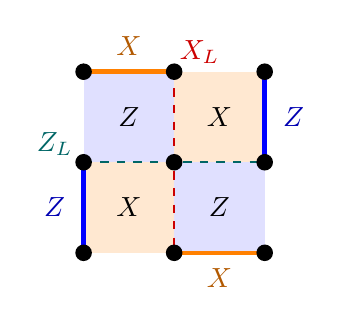
\begin{tikzpicture}[scale=1.15]
    % 上位に薄く各プラケットの塗りを置く
    \fill[blue!12] (0,1) rectangle (1,2);
    \fill[orange!18] (1,1) rectangle (2,2);
    \fill[orange!18] (0,0) rectangle (1,1);
    \fill[blue!12] (1,0) rectangle (2,1);
    % 境界の重み2生成元
    \draw[orange, ultra thick] (0,2) -- (1,2);
    \draw[orange, ultra thick] (1,0) -- (2,0);
    \draw[blue, ultra thick]   (0,1) -- (0,0);
    \draw[blue, ultra thick]   (2,2) -- (2,1);
    % 論理演算子（点線）
    \draw[red!80!black, thick, dashed]  (1,2) -- (1,1) -- (1,0);
    \draw[teal!80!black, thick, dashed] (0,1) -- (1,1) -- (2,1);
    % データ量子ビット
    \foreach \x in {0,1,2} {
      \foreach \y in {0,1,2} {
        \fill[black] (\x,\y) circle (2.6pt);
      }
    }
    % バルクプラケットのラベル
    \node at (0.5,1.5) {$Z$};
    \node at (1.5,1.5) {$X$};
    \node at (0.5,0.5) {$X$};
    \node at (1.5,0.5) {$Z$};
    % 境界プラケットのラベル
    \node[orange!70!black] at (0.5,2.28) {$X$};
    \node[orange!70!black] at (1.5,-0.28) {$X$};
    \node[blue!70!black]   at (-0.32,0.5) {$Z$};
    \node[blue!70!black]   at (2.32,1.5) {$Z$};
    % 論理演算子ラベル
    \node[red!80!black]  at (1.28,2.22) {$X_L$};
    \node[teal!80!black]  at (-0.32,1.2) {$Z_L$};
  \end{tikzpicture}
  \caption{$d=3$ の rotated surface code（9 データ量子ビット）。塗りと $X$/$Z$ の文字は生成元の型、太線は境界の重み 2 生成元、点線は論理演算子の代表元の一例を表します。}
  \label{fig:rotated_surface_d3}
\end{figure}

\subsection{境界と論理演算子}

図の中心にある 4 個の生成元は重み 4 で、市松模様のとおり $X$ 型と $Z$ 型が交互に配置されています。
格子の端では、はみ出す分のデータ量子ビットが存在しないため生成元の重みが 2 に落ち、これを\textbf{境界生成元}と呼びます。
rotated surface code には性質の異なる 2 種類の境界があります。

\begin{itemize}
  \item 境界の重み 2 生成元が $X$ 型になっている辺（図の上下）：これを \textbf{$X$ 境界}と呼びます。
  \item 境界の重み 2 生成元が $Z$ 型になっている辺（図の左右）：これを \textbf{$Z$ 境界}と呼びます。
\end{itemize}

本書の図と命名規約では、論理演算子をデータ量子ビットの鎖（同じ型のパウリ演算子を一列に並べた積）として実現し、\textbf{自分と同じ型と名付けた境界を結ぶ}代表元を選びます。rough/smooth や $X/Z$ 境界の呼称は文献の星・プラケット規約によって入れ替わり得るため、最終的な判定は名称ではなく、鎖が全スタビライザと可換で相補的な論理鎖と反可換かどうかで行います\cite{fowler2012surface}。
図では、$X_L$ が上下の $X$ 境界を結ぶ縦の鎖、$Z_L$ が左右の $Z$ 境界を結ぶ横の鎖として描かれています。
これは、同じ型のパウリ演算子どうしは常に可換なので、鎖が自分と同じ型の境界生成元とは自動的に可換になる（一方、反対の型の境界生成元とは、鎖がその境界を貫通しない限り可換にならない）という代数的な事情の帰結です。
図の $X_L$ と $Z_L$ はちょうど中央のデータ量子ビット 1 個だけを共有しており、この 1 点だけで反可換になることで、符号空間全体では正しく $X_LZ_L=-Z_LX_L$ が成り立ちます。

\subsection{$d=3$ という主戦場}

$d=3$ の rotated surface code は $[[9,1,3]]$ 符号で、生成元は重み 4 が 4 個、重み 2 が 4 個の合計 8 個です。
これは本書で繰り返し登場する最小構成であり、第7章以降で Stim を使って実際に構築し（\codepath{src/stages/01_mpp/src/ftqc} の幾何関数群）、第III部の格子手術や第12章の T ゲートに至るまで、一貫してこの $d=3$ パッチを土台にします。
$d$ を大きくすれば訂正能力（第3章で見た符号距離の効果）は上がりますが、量子ビット数は $n=d^2$ で増えるため、本書ではまず $d=3$ で語彙と手順を固め、必要な箇所でのみ距離を上げた場合の違いに触れる、という構成を取ります。

\begin{notebox}
  複数の $d=3$ パッチを隣接させ、境界どうしを一時的に結合・分離することで論理演算子どうしの合成測定を行う手法を\textbf{格子手術}と呼びます。
  境界の型（$X$ 境界か $Z$ 境界か）をどう合わせるかによって、測れる論理演算子の種類が決まります。
  幾何と生成元の組み合わせ規則の詳細は第10章（\codepath{src/stages/01_mpp/src/ftqc/geom_lattice_surgery.py} が対応）で扱い、本章では語彙の準備に留めます。
\end{notebox}

\section{魔法状態符号への布石（\texorpdfstring{$[[15,1,3]]$}{[[15,1,3]]}）}\label{sec:rm15}

\subsection{非 Clifford な資源の必要性}

表面符号のスタビライザ生成元は $X$ と $Z$ だけで書けるため、Hadamard・CNOT・$S$ ゲートといった Clifford 演算は、境界の操作や格子手術によって比較的単純に（多くの場合トランスバーサルに近い形で）実行できます。
しかし、Clifford 演算だけでは万能な量子計算はできません。
万能性のためには $T$ ゲート（あるいは Toffoli など）のような非 Clifford な演算が最低 1 種類必要です。

\begin{notebox}
  \textbf{Eastin--Knill の定理}：任意の単一物理サブシステムの誤りを検出できる有限次元の量子符号では、符号ブロック内の物理サブシステム同士を結合しない局所成分の積として作用するトランスバーサル論理ゲートだけで万能集合を構成できません。同じ物理ゲートを各サイトへかける場合だけに限らない定理です\cite{eastin2009transversal}。
  したがって、表面符号のようにトランスバーサルな Clifford 演算に適した符号だけでは $T$ ゲートを直接には実行できず、別の方法が必要になります。
\end{notebox}

その別の方法が\textbf{魔法状態}を用いたゲートテレポーテーションです。
あらかじめ $\ket{A} = T\ket{+}$ という特別な状態（魔法状態）を高い忠実度で用意しておけば、CNOT と測定、および測定結果に応じた $S$ 補正（既存の Clifford 演算だけ）を組み合わせることで、任意の論理量子ビットに $T$ ゲートを適用できます。
問題は、物理的に用意できる $\ket{A}$ には常に誤りが混じっており、そのままでは精度が不足することです。

\subsection{$[[15,1,3]]$ Reed–Muller 符号}

この精度不足を解決する標準的な方法が\textbf{魔法状態蒸留}です。
そこで使われる代表的な符号が、パラメータ $[[15,1,3]]$ の punctured quantum Reed--Muller CSS 符号で、古典 Reed--Muller 符号を土台に構成されます\cite{bravyi2005magic}。
$n=15$ 個の物理量子ビット、$k=1$ 個の論理量子ビット、符号距離 $d=3$ を持ち、$X$ 型・$Z$ 型それぞれの検査行列が古典 Reed–Muller 符号の生成行列・検査行列から具体的に書き下せる、という意味で表面符号と同じ CSS の枠組みに収まります。

この符号の重要な性質は、物理量子ビットへのトランスバーサルな $T$ または $T^\dagger$（論理演算の向きは符号・位相規約に依存）が論理 $T$ 型ゲートを実装することです（表面符号にはこの性質がなく、ここが両者の役割の違いです）。
この性質を利用して、15 個のノイズを含む $\ket{A}$状態を用意し、$[[15,1,3]]$ 符号の検査（シンドローム測定）を行い、シンドロームがすべて $0$ になった場合だけを採用する（\textbf{ポスト選択}する）ことで、出力される 1 個の $\ket{A}$ 状態の誤り率を、入力の誤り率 $p$ のおおむね 3 次
\begin{equation}
  p_{\mathrm{out}} \ \sim\ 35\, p^3
\end{equation}
まで抑制できます。ここで $35p^3$ は、独立同分布の入力 $Z$ 型魔法状態誤りを確率 $p$ で入れ、Clifford 操作と検査を理想化した模型の条件付き出力誤り率の先頭項です。距離が3という事実だけから係数35やこの確率式が決まるわけではありません\cite{bravyi2005magic}。
これを「15-to-1 蒸留」と呼びます。

\subsection{蒸留との接続}

本章で確認した通り、表面符号は Clifford 演算を効率よく実行するための符号であり、$[[15,1,3]]$ Reed–Muller 符号は非 Clifford な $T$ ゲートを実行するための資源（魔法状態）を高精度に用意するための、まったく別の符号です。
本書のハイブリッド構成（Stim によるスタビライザ回路のサンプリングと Qulacs による非 Clifford な状態ベクトル計算の併用）は、この 2 つの符号がそれぞれ担う役割の違いをそのまま反映しています。
$[[15,1,3]]$ 符号の検査行列の具体的な構成、蒸留のモンテカルロ検証、およびゲートテレポーテーション回路そのものは第12章（\codepath{src/stages/01_mpp/src/ftqc/t_gate.py} が対応）で扱い、本章ではその手前の語彙（$n,k,d$、CSS、トランスバーサル性）を確認するに留めます。

\section{まとめ}\label{ch4:summary}

\begin{itemize}
  \item スタビライザ形式は、互いに可換な生成元の集合 $\mathcal{S}$ によって符号空間を定義し、誤りとの可換・反可換関係からシンドロームを読み出す、量子誤り訂正符号の共通言語です。
  \item 論理演算子はノーマライザ $N(\mathcal{S})$ のうちスタビライザ群 $\mathcal{S}$ に属さない元であり、その最小重みが符号距離 $d$ を定めます。符号は $[[n,k,d]]$ の 3 つの整数で特徴づけられます。
  \item CSS 符号は生成元を $X$ 型と $Z$ 型に分離でき、可換性が $H_XH_Z^{\top}=0$ という古典的な条件に帰着します。シンドロームは成分別に表せますが、相関ノイズでは独立復号が最適とは限りません。
  \item rotated surface code は CSS 符号の具体例で、市松模様のプラケットと 2 種類の境界（$X$ 境界・$Z$ 境界）を持ち、論理演算子は同じ型の境界を結ぶ鎖として実現されます。$d=3$（$[[9,1,3]]$）が本書全体の主戦場です。
  \item スタビライザ操作だけでは万能計算にならず、Eastin--Knill の定理は単一符号のトランスバーサルゲートだけで万能集合を作れないことを述べます。$[[15,1,3]]$ Reed--Muller 符号による魔法状態蒸留は $T$ ゲート資源を供給します。
\end{itemize}

次章では、本章で固定した符号（特に表面符号）を時間軸に沿って動かし、符号サイクルの繰り返し、パウリフレーム追跡、Clifford と非 Clifford の切り分け、そして単体の符号だけでは扱えない場面（ストール）が統合シミュレータを必要とする理由を見ていきます。

\begin{exercise}
  \begin{enumerate}
    \item 3 ビット反復符号 $\mathcal{S}=\langle Z_0Z_1, Z_1Z_2\rangle$ について、$X_L=X_0X_1X_2$ がすべての生成元と可換であること、および $X_L$ が生成元の積では表せない（$\mathcal{S}$ に属さない）ことを確認しなさい。
    \item CSS 条件 $H_XH_Z^{\top}=0\pmod2$ が、$X$ 型生成元と $Z$ 型生成元の台の重なりが常に偶数個であることと同値であることを、$X$ と $Z$ の反交換関係から説明しなさい。
    \item 図~\ref{fig:rotated_surface_d3} の $d=3$ rotated surface code で、右下のデータ量子ビットに $Z$ 誤りが 1 個起きた場合、反転する生成元（シンドローム）はどれかを図から特定しなさい。また、その誤りが $X_L$ に何らかの影響を与えるかどうかを、$X_L$ と $Z$ の可換性から論じなさい。
    \item Eastin--Knill の定理が「単一のスタビライザ符号ではトランスバーサルな万能ゲート集合を持てない」と述べていることを踏まえ、表面符号と $[[15,1,3]]$ 符号という\textbf{2 つの符号}を併用する構成が、この定理をどのように回避しているかを 3 行程度で説明しなさい。
  \end{enumerate}
\end{exercise}

% Stage: — ／ 説明用コード: —
\chapter{エラー訂正フロー}\label{ch:qec_flow}

\begin{chaptergoal}
  \begin{itemize}
  \item シンドローム測定を時間軸上で繰り返す「符号サイクル」と、$T_1$ 緩和時間による制約を理解します。
  \item 物理的な即時訂正を避け、古典コンピュータ上でエラーを追跡する「パウリフレーム」の考え方を理解します。
  \item クリフォード操作がパウリフレーム追跡と相性がよい理由と、非クリフォード操作がその前提を崩す理由を理解します。
  \item 魔法状態テレポーテーションに伴うデコード遅延とストール問題を理解します。
  \item 層を横断する論理エラー率を評価するために、統合シミュレータが必要になる理由と本書全体の狙いを理解します。
  \end{itemize}
\end{chaptergoal}

第3章では、シンドローム測定を1回きりの操作として、いわば静止画のように取り上げました。
第4章では、その静止画の中身であるスタビライザ形式・符号距離・CSS条件・表面符号の幾何を確認しました。
本章では視点を変え、実際にFTQCで計算を実行する際にこの静止画がどのように\textbf{時間軸上で繰り返され}、論理演算とどう絡み合うのかを見ていきます。
符号サイクルの繰り返しと $T_1$ 制約、物理的な訂正を行わない代わりに古典ソフトウェアでエラーを追跡する仕組み（パウリフレーム）、クリフォード操作と非クリフォード操作の非対称性、そして非クリフォード操作にまつわるデコード遅延とストール問題を順に確認し、最後にこれらすべてを一つの評価軸でまとめるために本書がなぜハイブリッド型シミュレータを組み立てるのかを述べて、第I部を締めます。

\section{誤り訂正サイクルと \texorpdfstring{$T_1$}{T1} 制約}\label{sec:cycle_t1}

\subsection{符号サイクル}

第3章・第4章のシンドローム測定は、1回の測定でどれだけの情報が得られるかという説明に専念していました。
表面符号などの能動的な量子メモリでは、計算中も保存中もこの測定を周期的に繰り返します。
1回のシンドローム測定（パリティ検査）を行ってから次のシンドローム測定を行うまでの一続きの量子回路を、\textbf{符号サイクル}と呼びます。

論理量子ビットに何らかの論理演算を実行させている間も、演算をせずにただ情報を保持させている間（アイドリング）も、符号サイクルは休みなく繰り返し実行されます。
各サイクルの量子回路の内容は、実行中の論理演算の種類に応じて多少変化しますが、どの場合であっても、量子ビットが物理的に保持できる時間に対して十分短い時間で完了できる回路深さでなければならない、という制約は共通しています。

\subsection{$T_1$ 緩和時間との競合}

物理量子ビットが励起状態のエネルギーを失う振幅減衰の時定数を\textbf{$T_1$ 緩和時間}、位相コヒーレンスが失われる時定数を\textbf{$T_2$} と呼びます。Markov 的な単純模型では励起状態の生存確率は $\exp(-t/T_1)$ のように連続的に減衰し、$T_1$ を境に突然崩壊するわけではありません\cite{krantz2019guide}。

符号サイクルの役割は、この崩壊が訂正不可能なほど進行する前に誤りを検知することです。
振幅減衰だけを見た設計上の目安として、符号サイクル1回にかかる時間 $t_c$ は
\begin{equation}\label{eq:cycle_vs_t1}
  t_c \ll T_1
\end{equation}
となることが望まれます。ただしこれは閾値条件そのものではなく、$T_2$、漏れ、ゲート・測定誤り、相関誤りを含む1サイクル当たりの実効ノイズが、採用する符号とデコーダの閾値を下回ることが本質です\cite{krantz2019guide,dennis2002topological}。

もし符号サイクルの間隔を延ばしたり、サイクルそのものを休止したりすると、その休止時間中にも物理誤りは確率的に発生し続けます。
独立な Markov 誤りを仮定し、休止時間が各コヒーレンス時間より十分短い領域では、期待故障数は時間にほぼ比例して増えます。長時間や相関ノイズではこの線形近似は成り立たず、故障数が訂正能力を超える確率を評価する必要があります。
これが、能動的な表面符号メモリでは\textbf{論理演算を行っていないアイドリング中も符号サイクルを継続する}理由です。
データ量子ビットは、常にシンドローム測定という「保守作業」を受け続けることによって、はじめて論理情報を長時間保持できます。

\begin{notebox}
  古典のDRAMメモリも、電荷が漏れて情報が消えるのを防ぐために一定間隔で\textbf{リフレッシュ}を行います。
  符号サイクルによるアイドリングの保護は、この古典的なリフレッシュの量子版だと考えると直感的です。
  ただし量子の場合、リフレッシュのたびに情報を直接読み出す（測定する）わけではなく、第3章で見た間接測定＝シンドローム測定を使う点が異なります。
\end{notebox}

\section{パウリフレームと古典ソフトウェア追跡}\label{sec:pauli_frame}

\subsection{物理的な訂正をしないという選択}

符号サイクルでシンドロームが得られ、デコーダが観測結果と整合する訂正の同値類を選んだとしても、素朴には「推定した誤りを打ち消すパウリ操作を物理量子ビットに実際にかける」ことで訂正が完了すると考えたくなります。シンドロームだけから実際に起きた物理誤りを一意に知ることはできません。
しかし、この\textbf{物理的な訂正}には見過ごせないコストがあります。

\begin{itemize}
  \item 訂正操作そのものが、新たな物理誤りの追加源になり得る。
  \item デコードには一定の時間がかかるため（5.4節のストール問題）、訂正操作の完了を待つ間、次の符号サイクルの開始が遅れる。
  \item 論理演算のたびに関係する全量子ビットへ訂正をかけ直すのは非効率である。
\end{itemize}

FTQCの実用的なアーキテクチャでは、多くのパウリ補正を直ちに物理適用せず、後続ゲートと測定の解釈へ繰り延べられます。
代わりに、デコーダが選んだ訂正を適用したものとして解釈するためのパウリ演算子を\textbf{古典コンピュータ上の帳簿}として記録し続け、必要になった時点（測定結果の解釈や論理読み出しの直前など）で帳尻を合わせます。
この帳簿を\textbf{パウリフレーム}と呼びます。

\subsection{パウリフレームが成立する根拠}

パウリフレームが機能する根拠は、クリフォード操作が持つ次の性質です。
クリフォード操作 $U_C$ と任意のパウリ演算子 $P$ に対して
\begin{equation}\label{eq:clifford_conj}
  U_C P = P' U_C, \qquad P' = U_C P U_C^\dagger
\end{equation}
が成り立ち、$P'$ は符号（$\pm1$ の位相）を除いて再びパウリ演算子になります。
これは「$U_C$ がパウリ群を自分自身へ写す」という性質そのもので、クリフォード操作の定義です\cite{aaronson2004stabilizer}。

いま、本来の状態 $\ket\psi$ にパウリ誤り $E$ が乗った状態 $E\ket\psi$ にクリフォード操作 $U_C$ を適用したとします。式\eqref{eq:clifford_conj}より
\begin{equation}
  U_C \bigl(E\ket\psi\bigr)
  = \bigl(U_C E U_C^\dagger\bigr) U_C \ket\psi
  = E' \, U_C\ket\psi, \qquad E' = U_C E U_C^\dagger
\end{equation}
となります。右辺は「誤りのない状態 $\ket\psi$ に $U_C$ をかけたあと、別のパウリ誤り $E'$ が乗っている」と読めます。つまり、

\begin{quote}
  「誤りが乗った状態に演算をかけた結果」と「誤りのない状態に演算をかけたあと、演算に応じて誤りの種類を古典的に付け替えた結果」は、量子状態として完全に等価である
\end{quote}

ということです。この付け替えは行列の積を計算するだけの古典計算であり、実際の量子ビットには一切手を触れません。

この関係を毎サイクル繰り返し適用すれば、量子デバイスは物理補正を毎回実行せずに演算を続けられ、古典コンピュータの側だけがデコーダの選んだ訂正代表を表すパウリ演算子 $F$（各量子ビットに $I,X,Y,Z$ のいずれかを割り当てたもの）を式\eqref{eq:clifford_conj}に従って更新できます。この $F$ が\textbf{パウリフレーム}です。
シンドローム測定の測定値（レコード）についても、その値が本来ゼロになるはずかどうかを、実際の測定値とパウリフレーム $F$ とを比較して古典的に判定します。

\begin{notebox}
  パウリフレームは、量子ビットの「実体」を書き換える代わりに、実体と設計図のあいだの\textbf{ずれ}だけを古典コンピュータに覚えさせておく仕組みだと考えると直感的です。
  設計図どおりに動いていないと分かった時点でいちいち実体を直しに行くのではなく、「今どれだけずれているか」を台帳に記録しておき、最終的な読み出しや論理演算の解釈のときだけその台帳を参照して辻褄を合わせます。
\end{notebox}

\section{論理ゲートの分類とクリフォードの特異性}\label{sec:gate_classification}

\subsection{クリフォードと非クリフォード}

論理演算は、パウリフレームとの相性という観点から大きく2種類に分類されます。

\begin{itemize}
  \item \textbf{クリフォード操作}（$H$、$S$、CNOT、およびこれらの合成）：式\eqref{eq:clifford_conj}のとおり、パウリ演算子をパウリ演算子（符号を除く）に写します。
  \item \textbf{非クリフォード操作}（$T$ ゲートなど）：この写像がパウリ群の外に出てしまい、単純な古典的付け替えでは追跡できません。
\end{itemize}

シンドローム測定の回路自体も、スタビライザ状態の初期化、Clifford ゲート、Pauli 測定という\textbf{スタビライザ操作}で構成されています。初期化と測定はユニタリな Clifford ゲートではありません。
したがって、符号サイクルを回している間に生じるパウリ誤りは、常に式\eqref{eq:clifford_conj}の関係でパウリフレームへ吸収できます。
これが、誤り訂正サイクルとクリフォードな論理演算を、量子デバイスを止めることなく古典ソフトウェアだけで整合させられる理由です。

\subsection{$T$ ゲートがパウリ群を保たないことの確認}

非クリフォードの代表例である $T=\operatorname{diag}(1,\ee^{\ii\pi/4})$ が、なぜパウリ演算子をパウリ演算子に写さないのかを具体的に確かめます。
$TXT^\dagger$ を計算すると
\begin{equation}\label{eq:t_not_clifford}
  TXT^\dagger
  = \begin{pmatrix} 0 & \ee^{-\ii\pi/4} \\ \ee^{\ii\pi/4} & 0 \end{pmatrix}
  = \cos\frac{\pi}{4}\, X + \sin\frac{\pi}{4}\, Y
  = \frac{1}{\sqrt2}(X+Y)
\end{equation}
となります。右辺はパウリ演算子 $X$ と $Y$ の実数係数の重ね合わせであり、単一のパウリ演算子ではありません。
したがって $T$ は式\eqref{eq:clifford_conj}の意味でのクリフォード条件を満たさず、$T$ ゲートの前後でパウリフレームを単純な文字列の付け替えとして押し出すことができません。

このことは、より根本的な事実、すなわちトランスバーサル操作だけではユニバーサルな計算ができないという定理（第4章で触れた話題と表裏一体）とも整合します。
クリフォード操作だけでは複雑なアルゴリズムを実行できないため非クリフォード操作は必須ですが、式\eqref{eq:t_not_clifford}が示すとおり、それを安全に実行するにはパウリフレームの付け替えとは別の仕掛けが必要になります。次節でこれを見ます。

\section{非クリフォード操作のデコード遅延とストール問題}\label{sec:stall}

\subsection{ゲートテレポーテーションとフィードフォワード}

論理 $T$ ゲートは、物理量子ビットに直接かけることができません。
代わりに、あらかじめ $T\ket{+}$ に相当する\textbf{魔法状態}を論理レベルで用意し、対象の論理量子ビットと量子もつれさせたうえで対象を測定する\textbf{ゲートテレポーテーション}という手法で実行します\cite{bravyi2005magic, gidney2019factory}（符号化・蒸留の具体的な手順は第III部で扱います）。

この手順を論理レベルの回路として書くと図\ref{fig:t_teleport}のようになります。

\begin{figure}[htbp]
  \centering
  \begin{quantikz}
    \lstick{$\ket{\psi}_L$}          & \ctrl{1} & \gate{S^{m}} & \rstick{$T\ket{\psi}_L$} \\
    \lstick{$\ket{A}_L=T\ket{+}_L$}  & \targ{}  & \meter{}     &
  \end{quantikz}
  \caption{$T$ ゲートテレポーテーションの概念図（論理レベル）。データ側を制御、魔法状態 $\ket{A}_L$ を標的として $\mathrm{CNOT}$ をかけたのち、\textbf{魔法状態側を $Z$ 基底で測定}します。測定結果 $m\in\{0,1\}$ に応じて、\textbf{データ側}に補正 $S^m$ をかけるかどうかが決まります（フィードフォワード）。目的の状態はデータ側の線に得られます。}
  \label{fig:t_teleport}
\end{figure}

同図のとおり、測定結果 $m$ に応じて後続に補正操作 $S^m$ をかけるかどうかが変わります。
この「測定結果を見てから後続の回路の内容を選ぶ」処理を\textbf{フィードフォワード}と呼びます。

測定を含む Clifford 実装にも結果依存の分岐はあり得ますが、結果依存の\emph{Pauli}補正なら通常はパウリフレームへ吸収できます。一方 $S^m$ は Pauli ではないため、通常のパウリフレームには追加できません。物理的または適応的に実行するか、より一般の\textbf{Clifford frame}として追跡します\cite{chamberland2018frame}。
しかし、$m$ の値を決める測定そのものにも物理誤りが乗っており、真の $m$ を確定するには、その符号サイクルまでの\textbf{シンドローム測定の結果をすべて集めてデコードを完了させる}必要があります。
続けて別の非クリフォード操作が来る場合、どちら向きの補正が要るかを誤ると、以降のパウリフレームの管理そのものが破綻してしまいます。
そのため、後続操作の選択がこの値に依存する地点では、\textbf{必要なデコードを完了させて確定した値を使う}場面が生じます。Clifford frame、選択的テレポーテーション、バッファリングなどで依存関係を先送りできる設計もあり、すべての非 Clifford 境界が必ず停止点になるわけではありません\cite{chamberland2018frame}。

\subsection{リアクション時間とストール}

制御装置が論理パウリ測定（あるいは非クリフォード操作の一部としての測定）を送出してから、デコードを経て確定した測定値が返るまでの時間を\textbf{リアクション時間}と呼びます。
符号サイクル自体は1回あたり短時間（5.1節の $t_c$）で完了しますが、シンドロームから誤りを推定するデコード計算は一般に計算量的に重い問題であり、符号サイクルよりずっと長くかかることがあります。
実際のリアクション時間は、符号距離、デコーダ、古典ハードウェア、制御系の通信経路に依存します。

このリアクション時間の間、量子デバイス側は次の非クリフォード操作へ進めず待たされます。この待機を\textbf{ストール}と呼びます。
ストールしている間も、待機中の論理量子ビットに対する符号サイクルは（5.1節のとおり）回り続けますが、もしストール時間が $T_1$ に対して無視できないほど長くなれば、待機中の量子ビットに蓄積する実効的な誤り率が上昇し、論理エラー率の悪化につながります。
つまりストール問題は、「符号サイクルは $T_1$ より十分短くなければならない（式\eqref{eq:cycle_vs_t1}）」という制約と、「非クリフォードの境界ではデコードの完了を待たなければならない」という制約が正面から衝突する点に生じる、FTQCアーキテクチャ特有のボトルネックです。

\subsection{3つのボトルネックとしての整理}

以上の議論は、FTQC全体の実行時間を大まかに次の3種類のボトルネックのどれかとして捉える見方につながります。

\begin{itemize}
  \item \textbf{魔法状態の供給}：必要な魔法状態数 $N_M$ と生成周期 $T_M$ の積 $N_M T_M$。
  \item \textbf{リアクションの連鎖}：非クリフォード操作どうしの依存関係の長さ $N_R$ とリアクション時間 $T_R$ の積 $N_R T_R$。
  \item \textbf{符号サイクルの繰り返し}：計算全体で必要な符号サイクル数 $N_C$ と、サイクル時間 $T_C$ の積 $N_C T_C$。
\end{itemize}

このうちどれか1つが極端に支配的であれば、計算機の設計とアプリケーションの要求がかみ合っていないことを意味します。
ボトルネックの所在を特定し、デコーダの高速化・コンパイル時の非クリフォード演算の並列化・魔法状態工場の規模調整などで手当てするのが、FTQCシステム設計の実務的な課題です。
本書のシミュレータ（第III部以降）でも、この3つの視点は論理エラー率・実行時間の評価軸として繰り返し登場します。

\section{統合評価環境の必要性と本書の狙い}\label{sec:integrated_sim}

\subsection{層を横断する論理エラー率}

ここまでで確認したFTQCの実行フローは、少なくとも次の3層が互いに絡み合って動いています。

\begin{itemize}
  \item \textbf{量子誤り訂正層}：符号サイクルによるシンドローム測定と、そこからのデコード（第II部以降）。
  \item \textbf{クリフォード論理演算層}：パウリフレームによる古典的な追跡（本章5.2–5.3節）。
  \item \textbf{非クリフォード層}：魔法状態を介したゲートテレポーテーションとフィードフォワード（本章5.4節）。
\end{itemize}

最終的にアプリケーションが気にする量は、これら3層すべてを通過したあとの\textbf{論理エラー率}です。
ところが、既存の評価環境は層ごとに分断されています。
たとえば第6章で導入する Stim はスタビライザ回路の高速シミュレーションに特化した強力なツールですが、扱えるのはクリフォード演算に限られたクリフォードシミュレータです。
非クリフォード操作を含む厳密な量子状態を追いたければ状態ベクトルシミュレータが必要になりますが、これは量子ビット数に対して指数的なコストがかかり、量子誤り訂正符号が要求する物理量子ビット数をそのまま扱うことはできません。
つまり、単独のツールでは3層をまとめて評価できないというのが現状です。

\subsection{Stim + 状態ベクトル + パウリフレームのハイブリッド}

本書で組み立てるシミュレータは、この3層を次のように役割分担させることで、それぞれの限界を回避します。

\begin{itemize}
  \item \textbf{Stim}：スタビライザ回路を高速にサンプリングし、検出器誤りモデルを生成します。復号そのものは PyMatching や BP+OSD など外部デコーダが担います\cite{gidney2021stim}。
  \item \textbf{Qulacs（状態ベクトル）}：魔法状態や非 Clifford 操作が関わる、実装が選んだ小規模な論理状態を状態ベクトルとして追跡します。
  \item \textbf{パウリフレーム（ソフトウェア追跡）}：本章で見た古典的な帳簿を実際にプログラム上で実装し、上の2つのバックエンドの結果を、実際に物理操作をかけ直すことなく1つの整合した論理エラー率へまとめ上げます。
\end{itemize}

つまり「大部分をクリフォードシミュレータで高速に流し、非クリフォードが絡む狭い範囲だけを状態ベクトルで厳密に扱い、両者のつなぎ目をパウリフレームで古典的に処理する」というのが、本書のハイブリッド型アーキテクチャの骨格です。
第I部で確認した4つの制約（第2章）、シンドローム測定の必然性（第3章）、符号の幾何（第4章）、そして本章で見たフロー全体は、いずれもこのハイブリッド構成がなぜ必要かを説明するための土台でした。

\subsection{読書の地図：Stage 01 から F へ}

本書はこのシミュレータを一気に完成形として提示するのではなく、次の表のように段階（Stage）を踏んで組み立てます。

\begin{center}
\begin{tabular}{cll}
\hline
Stage & 到達点 & 対応する部 \\
\hline
基礎 & FTQC と誤り訂正の考え方 & 第I部 \\
01 & 現象論 MPP による論理演算の骨格 & 第II・III部 \\
02 & 回路レベル格子手術 & 第IV部 \\
03 & $d=3$ 固定の統合シミュレータ & 第V部 \\
\hline
\end{tabular}
\end{center}

第II部ではまず、この骨格の入口として Stim の基本的な使い方（第6章）、表面符号パッチの作り方（第7章）、デコードと評価基準の考え方（第8章）を押さえます。
そこから第III部以降で、本章で述べたパウリフレーム・クリフォード/非クリフォードの区別・ストール対策の考え方を、実際に動くコードとして段階的に積み上げていきます。
本章では実装の詳細には踏み込まず、以降の章でコードとして再会するための見取り図を示すことに専念しました。

\subsection{統合評価環境の 3 つの目的と本書の到達範囲}\label{sec:integrated_goals}

層を横断する統合評価環境には、個別のツールでは見えない問題を調べる役割があります。
目的は次の 3 つに整理できます。
一つ目は、$T$ ゲートのたびに生じる「測定 $\to$ 古典側への転送 $\to$ デコード $\to$ フィードフォワード」の往復時間が、量子ビットの寿命に対してどれだけ余裕を持つかを定量化することです。
二つ目は、論理的な計算時間だけでなく、魔法状態の生成時間やストールによる待ちを含めた実効的な計算時間を評価し、デコーダの高速化・通信帯域・工場の並列度のどこに資源を投じるべきかを判断することです。
三つ目は、測定結果によって回路が変わる環境で、限られた接続性のもとでの演算の配置と経路を決めるコンパイラを試すテストベッドになることです。

本書のシミュレータがこの 3 つのどこまでを扱い、どこから先を扱わないかを表\ref{tab:ch5_integrated_goals}に示します。
本書は実時間を持たない論理層のシミュレータなので、時間に関わる量はラウンド数と解析的なコストモデルで扱い、実機の遅延そのものは測りません。

\begin{table}[htbp]
  \centering
  \caption{本書が扱う評価軸と対象外の実測量}
  \label{tab:ch5_integrated_goals}
  \begin{tabularx}{\textwidth}{>{\raggedright\arraybackslash}p{0.25\textwidth}X X}
    \hline
    \textbf{評価軸} & \textbf{本書で扱うもの} & \textbf{本書で扱わないもの} \\
    \hline
    論理誤り & 検出器、復号結果、論理残差 & 実機での論理誤り率の保証 \\
    回路コスト & ラウンド数、補助量子ビット、簡易モデル & 実時間のデコード・通信遅延 \\
    非 Clifford 操作 & 魔法状態、ゲートテレポーテーション、QPD & 実機の工場運用・資源配分 \\
    \hline
  \end{tabularx}
\end{table}

\section{まとめ}\label{ch5:summary}

\begin{itemize}
  \item シンドローム測定を1回きりの静止画としてでなく、\textbf{符号サイクル}として時間軸上に繰り返す視点が必要です。$t_c\ll T_1$ は有用な設計目安ですが、実効ノイズには $T_2$、ゲート・測定誤り、漏れ、相関も含まれます。
  \item FTQCは物理的な即時訂正を避け、代わりに\textbf{パウリフレーム}という古典的な帳簿でエラーを追跡します。この仕組みは、クリフォード操作がパウリ演算子をパウリ演算子に写す性質（式\eqref{eq:clifford_conj}）に支えられています。
  \item 非クリフォード操作（$T$ ゲート）はこの性質を持たず（式\eqref{eq:t_not_clifford}）、魔法状態を介したゲートテレポーテーションとフィードフォワードによって実行されます。
  \item デコードにかかる時間（リアクション時間）が符号サイクルより長いため、非クリフォード操作の境界で計算がストールする可能性があり、これがFTQCの主要なボトルネックのひとつです。
  \item 量子誤り訂正・クリフォード論理演算・非クリフォード層を横断して論理エラー率を評価するには、Stim・状態ベクトル・パウリフレームを組み合わせたハイブリッドシミュレータが必要であり、これが本書全体の狙いです。
\end{itemize}

第I部はここで一区切りです。次章からは第II部に入り、実際に手を動かしてStimの基本的な使い方から本書のシミュレータの構築を開始します。

\begin{exercise}
  \begin{enumerate}
    \item $t_c\ll T_1$ が有用な設計目安である理由と、それだけでは閾値以下を保証しない理由を、アイドリング中の $T_2$、ゲート・測定誤りにも触れて説明しなさい。
    \item クリフォード操作 $U_C$ とパウリ演算子 $E$ について、$U_C(E\ket\psi) = E' U_C \ket\psi$（$E'=U_CEU_C^\dagger$）が成り立つことが、パウリフレーム追跡にとってなぜ本質的なのかを一文で説明しなさい。
    \item 式\eqref{eq:t_not_clifford}の計算を確認し、$T$ ゲートが式\eqref{eq:clifford_conj}の意味でクリフォードでないことを、$TZT^\dagger$ についても同様に確かめなさい。
    \item リアクション時間がストールを引き起こす条件を、符号サイクル時間・$T_1$・デコード時間の関係として説明し、ストールを緩和する方法を1つ挙げなさい。
  \end{enumerate}
\end{exercise}

% ----- 第II部 -----
\part{道具立て — Stim と最初の論理量子ビット}\label{part:tools}

% Stage: 01 入口 ／ 説明用コード: Stim / src/stages/01\_mpp/src/ftqc
\chapter{Stim の使いかた}\label{ch:stim}

\begin{chaptergoal}
  \begin{itemize}
  \item Stim の \texttt{Circuit} と \texttt{TableauSimulator} を使い、量子回路を組み立ててノイズなしで動作確認できるようになります。
  \item \texttt{DETECTOR}・\texttt{OBSERVABLE\_INCLUDE}・測定レコードの意味を理解し、検出器が「決定論的であるべき量」であることを説明できます。
  \item detector sampler と生のサンプラの違いを理解し、真理値表検証とデコードのそれぞれに適切な方を選べます。
  \item \texttt{detector\_error\_model} の役割と \texttt{allow\_gauge\_detectors} の落とし穴を理解し、本書がこれを使わない理由を説明できます。
  \item PyMatching・BP+OSD・qulacs がハイブリッド型シミュレータの中でどの役割を担うかを把握します。
  \end{itemize}
\end{chaptergoal}

第5章では、符号サイクルを周期的に繰り返してシンドロームを取得するという時間軸上の構造を確認しました。
本章では、その構造を実際にプログラムとして書き下すための道具である Stim（対象バージョン 1.16.0）を扱います\cite{gidney2021stim, stim2026doc}。
Stim はスタビライザ回路を高速にサンプリングできるシミュレータであり、本書の主エンジンとして第II部以降のほぼ全ての章で使われます。
本章の目的は Stim の全機能を網羅することではなく、\codepath{src/stages/01_mpp/src/ftqc/} のコードを読み解くために最低限必要な API（回路構築、検出器、観測量、サンプラ、DEM、デコーダ連携）を実装可能な粒度で押さえることです。

\begin{notebox}
  Stage: \textbf{01}。
  説明用コードは Stim の最小例および \codepath{src/stages/01_mpp/src/ftqc/} を用います。
  本章のコード引用はすべて \codepath{src/stages/01_mpp/src/ftqc/} 内の既存ファイルから採ったものであり、架空の関数名は用いません。
\end{notebox}

\section{インストールと基本}\label{sec:stim_basics}

\subsection{インストール}

本書は Python の実行に uv 環境を使います。導入手順の詳細は付録\ref{app:setup}に譲ります。Stage 01 の依存関係とロック情報は \codepath{src/stages/01_mpp/pyproject.toml} と \codepath{src/stages/01_mpp/uv.lock} で管理します。

\begin{lstlisting}[caption={pyproject.toml の依存関係の記法（抜粋）}]
[project]
dependencies = ["numpy", "scipy", "matplotlib", "stim", "pymatching", "qulacs"]
\end{lstlisting}

\texttt{stim} が本章の主役、\texttt{pymatching} と \texttt{stimbposd} は6.5節のデコーダ、\texttt{qulacs} は非 Clifford の状態ベクトル計算に使います。
\texttt{qulacs} はオプショナルな依存であり、無い場合は NumPy 状態ベクトルにフォールバックする実装が \codepath{src/stages/01_mpp/src/ftqc/hybrid_ftqc_runtime.py} にあります（13章で詳しく扱います）。

\subsection{Circuit}

\texttt{stim.Circuit} は量子回路を表すオブジェクトで、\texttt{append} メソッドでゲート・測定・ノイズ命令を1つずつ追加していきます。

\begin{lstlisting}[language=Python, caption={最小のベル状態回路}]
import stim

c = stim.Circuit()
c.append("H", [0])
c.append("CX", [0, 1])
c.append("M", [0, 1])
print(c)
\end{lstlisting}

\codepath{src/stages/01_mpp/src/ftqc/} の実装では、回路を1命令ずつ手で組み立てる代わりに \texttt{stim.Circuit.generated} で組み込みの符号ファミリを生成することも多く使われます。
たとえば \codepath{src/stages/01_mpp/src/ftqc/ftqc_toy.py} の \texttt{stage1\_qec} 関数は次のように rotated surface code のメモリ実験回路を得ています。

\begin{lstlisting}[language=Python, caption={src/stages/01\_mpp/src/ftqc/ftqc\_toy.py の抜粋（stage1\_qec 内）}]
circuit = stim.Circuit.generated(
    "surface_code:rotated_memory_z",
    distance=distance,
    rounds=rounds,
    after_clifford_depolarization=p,      # 2量子ビットゲート後の脱分極
    before_measure_flip_probability=p,    # 測定エラー
)
\end{lstlisting}

一方、\codepath{src/stages/01_mpp/src/ftqc/transversal_cnot.py} や \texttt{clifford\_ft\_full.py} のように、検出器やスタビライザを自前で管理したい場合は \texttt{MPP}（multi-Pauli product measurement、多体 Pauli 測定）命令で回路を手組みします。
\texttt{MPP} で複数量子ビットにわたる Pauli 積 $X_0 X_1$ や $Z_1Z_2$ を1回の測定で読み出せるため、表面符号のスタビライザ測定を簡潔に書けます（第7章で詳しく扱います）。

\subsection{TableauSimulator}

ノイズを含まない Clifford 回路を厳密に追跡したい場合は \texttt{stim.TableauSimulator} を使います。
\codepath{src/stages/01_mpp/src/ftqc/hybrid_ftqc_runtime.py} の \texttt{StimCliffordBackend} は、ハイブリッドランタイムの Clifford 専用バックエンドとしてこれを利用しています。

\begin{lstlisting}[language=Python, caption={src/stages/01\_mpp/src/ftqc/hybrid\_ftqc\_runtime.py の抜粋（StimCliffordBackend）}]
self.sim = stim.TableauSimulator()
...
circ = self._stim.Circuit()
circ.append(stim_name, [int(t) for t in targets])
if hasattr(self.sim, "do"):
    self.sim.do(circ)
\end{lstlisting}

\texttt{TableauSimulator} は状態ベクトルを持たずスタビライザ表（タブロー）だけを更新するため、量子ビット数が増えても Clifford 演算であれば高速に動きます。
非 Clifford な T ゲートを扱う際にはこの表現では追えないため、6.5節で述べる状態ベクトルバックエンド（qulacs／NumPy）に処理を渡します。

\section{DETECTOR・OBSERVABLE\_INCLUDE・レコード}\label{sec:detectors_obs}

\subsection{測定レコード}

Stim は \texttt{M}（単一量子ビット測定）や \texttt{MPP}（多体 Pauli 測定）を実行するたびに、その結果を\textbf{測定レコード}という連番付きの列に積み重ねます。
\texttt{DETECTOR} や \texttt{OBSERVABLE\_INCLUDE} は、このレコードのうち「どの測定結果を XOR するか」を \texttt{stim.target\_rec} で指定します。
\texttt{target\_rec} の引数は現在位置からの負の相対オフセットで、直前の測定が \texttt{-1}、その1つ前が \texttt{-2} という具合です。
絶対インデックス \texttt{a} と現在の測定総数 \texttt{mc} から相対オフセットへ変換する次のパターンが \codepath{src/stages/01_mpp/src/ftqc/} のほぼ全ファイルで繰り返し使われます。

\begin{lstlisting}[language=Python, caption={絶対インデックス→相対オフセット変換（各ファイル共通の慣用句）}]
rr = lambda a: stim.target_rec(a - mc)
\end{lstlisting}

\subsection{検出器の意味}

\texttt{DETECTOR} は、指定した測定レコードたちの XOR が\textbf{ノイズがなければ常に同じ値（通常は0）になる}という主張を Stim に登録する命令です。
言い換えると、検出器は「回路の理想的な振る舞いから決定論的に求まる量」でなければなりません。
ノイズが入ったときに、この決定論的な値からずれた（つまり検出器が1になった）ことをもって「どこかで誤りが起きた」と判定するのがシンドローム測定の実装そのものです。

第9章で扱う生成子追跡（generator tracking）の実装 \codepath{src/stages/01_mpp/src/ftqc/clifford_ft_full.py} では、この決定論性を「同じインデックスの生成子を連続する2ラウンドで比較する」という一様な規則だけで実現しています。

\begin{lstlisting}[language=Python, caption={src/stages/01\_mpp/src/ftqc/clifford\_ft\_full.py の抜粋（DETECTOR の一様規則）}]
for gi, (_, _, _, typ) in enumerate(gens):
    if typ == "Z":                      # round 0: Z 型は決定論的
        c.append("DETECTOR", [rr(ridx[(0, gi)])])
for r in range(1, R):                   # 一様規則: 同インデックス連続比較
    for gi in range(len(gens)):
        c.append("DETECTOR", [rr(ridx[(r, gi)]), rr(ridx[(r - 1, gi)])])
\end{lstlisting}

ゲート（H や CNOT）を挟んでも、生成子そのものを共役変換して追いかけているため、round $r$ の生成子は round $r-1$ の生成子に一致し、ノイズなしでは検出器が恒等的に0になります。
これは「ゲートごとに検出器の張り替えルールを場当たり的に書く」設計とは対照的で、6.4節で述べる gauge 検出器を生まないための鍵になります。

\subsection{論理オブザーバブル}

\texttt{OBSERVABLE\_INCLUDE} は、測定レコードの XOR を「論理量子ビットの読み出し値」として登録する命令です。
デコーダの予測とこの観測量の理想値を比較した差が論理エラーになります。
\codepath{src/stages/01_mpp/src/ftqc/transversal_cnot.py} では、制御・標的パッチそれぞれの論理 $Z_L$ を次のように登録しています。

\begin{lstlisting}[language=Python, caption={src/stages/01\_mpp/src/ftqc/transversal\_cnot.py の抜粋}]
c.append("OBSERVABLE_INCLUDE", [rr(drec[('c', q)]) for q in ZL], 0)
c.append("OBSERVABLE_INCLUDE", [rr(drec[('t', q)]) for q in ZL], 1)
\end{lstlisting}

\texttt{OBSERVABLE\_INCLUDE} の第2引数（ここでは \texttt{0}, \texttt{1}）は観測量番号で、複数の論理量子ビットを1つの回路の中で別々に追跡するために使われます。

\section{detector sampler と生のサンプラ}\label{sec:samplers}

Stim の回路から結果を取り出す方法には、目的の異なる2種類のサンプラがあります。

\begin{itemize}
  \item \textbf{生のサンプラ}（\texttt{circuit.compile\_sampler()}）：すべての測定レコードをそのままビット列として返します。デコード前の「論理値そのもの」を見たいとき、すなわち真理値表検証や参照分布との比較に向いています。
  \item \textbf{detector sampler}（\texttt{circuit.compile\_detector\_sampler()}）：検出器の値（シンドローム）と観測量の値を別々に返します。デコード・論理エラー率の評価に向いています。
\end{itemize}

\codepath{src/stages/01_mpp/src/ftqc/transversal_cnot.py} の真理値表検証は、ノイズを切った回路の生のサンプルを使って「制御ビットは不変、標的ビットは XOR」という代数的な性質を確認しています。

\begin{lstlisting}[language=Python, caption={src/stages/01\_mpp/src/ftqc/transversal\_cnot.py の抜粋（verify\_truth\_table）}]
circ, nm = build_cnot_circuit(noise=False, control_one=c1, target_one=t1)
ref = np.array(circ.without_noise().reference_sample(), int)
cz = _logical_z(ref, nm, 'c')
tz = _logical_z(ref, nm, 't')
\end{lstlisting}

\texttt{without\_noise()} はノイズ命令を取り除いた回路を返し、\texttt{reference\_sample()} はその決定論的な1サンプルを取得します。
一方、ノイズを入れたままデコードして論理エラー率を測る場面では \texttt{compile\_detector\_sampler} を使います。

\begin{lstlisting}[language=Python, caption={src/stages/01\_mpp/src/ftqc/transversal\_cnot.py の抜粋（decode）}]
def decode(circ, shots=40000):
    det, obs = circ.compile_detector_sampler().sample(shots, separate_observables=True)
    dem = circ.detector_error_model(decompose_errors=True)
    matcher = pymatching.Matching.from_detector_error_model(dem)
    pred = matcher.decode_batch(det)
    res = obs ^ pred
    return res[:, 0].mean(), res[:, 1].mean()
\end{lstlisting}

\texttt{separate\_observables=True} を指定すると、戻り値が検出器ビット \texttt{det} と観測量ビット \texttt{obs} に分かれます。
\texttt{det} をデコーダに渡して予測 \texttt{pred} を得て、\verb|obs ^ pred| が0でなければ論理エラーが起きたと判定します。
この構図（サンプル → DEM → デコーダ → \texttt{obs} との比較）は、本書の全ての Stage で繰り返し登場する基本パターンです。

\section{detector\_error\_model と allow\_gauge\_detectors}\label{sec:dem_gauge}

\subsection{DEM の役割}

\texttt{circuit.detector\_error\_model()} は、回路中のノイズ命令1つ1つを「どの検出器とどの観測量を反転させるか」という誤りメカニズムの集合（detector error model、DEM）へ変換します。
これにより、量子回路のデコードを古典的なグラフ上の最小重みマッチング問題（あるいはより一般のデコード問題）に落とし込めます。

\texttt{decompose\_errors} 引数は、DEM をどこまで単純化するかを指定します。

\begin{itemize}
  \item \texttt{decompose\_errors=True}：各誤りメカニズムを、検出器を2つだけ反転させる素なエッジ（graphlike）に分解しようとします。分解に成功すれば PyMatching（MWPM）が使えます。
  \item \texttt{decompose\_errors=False}：分解を行わず、3つ以上の検出器を同時に反転させるハイパーエッジも含めた生の DEM を返します。graphlike に分解できない回路（H を含む Clifford など）では BP+OSD にこちらを渡します。
\end{itemize}

\codepath{src/stages/01_mpp/src/ftqc/clifford_ft_full.py} の \texttt{decode} メソッドは、まず graphlike 分解を試み、失敗したら（\texttt{ValueError}）BP+OSD にフォールバックするという構成になっています（詳細は6.5節）。

\subsection{gauge 検出器とその落とし穴}

DETECTOR を組み立てる際、指定した測定レコードの XOR が実は理想回路でも決定論的に定まらない（測定ごとに0と1のどちらも出る）ことがあります。
このような検出器を\textbf{gauge 検出器}と呼びます。
gauge 検出器が生じる典型的な原因は、検出器の張り替えルールの取りこぼしです。
たとえば \codepath{src/stages/01_mpp/src/ftqc/transversal_cnot.py} では、transversal CX の直後にどちらのパッチのどの安定化子が広がるかを踏まえて前ラウンドの測定値をクロス境界補正として混ぜ込む必要があります。

\begin{lstlisting}[language=Python, caption={src/stages/01\_mpp/src/ftqc/transversal\_cnot.py の抜粋（クロス境界補正）}]
if remap and boundary:
    if typ == "X" and patch == 'c':       # S_X^C -> S_X^C·S_X^T
        tg.append(rr(ridx[(r - 1, 't', si)]))
    if typ == "Z" and patch == 't':       # S_Z^T -> S_Z^C·S_Z^T
        tg.append(rr(ridx[(r - 1, 'c', si)]))
\end{lstlisting}

この補正の有無で検出器の決定論性が変わることを、同ファイルの \texttt{verify\_boundary\_remap} がノイズなし回路のサンプルだけで確認しています。

\begin{lstlisting}[language=Python, caption={src/stages/01\_mpp/src/ftqc/transversal\_cnot.py の抜粋（verify\_boundary\_remap）}]
def verify_boundary_remap():
    res = {}
    for rm in (False, True):
        circ, _ = build_cnot_circuit(noise=False, control_one=True, remap=rm)
        det, _ = circ.compile_detector_sampler().sample(100, separate_observables=True)
        res[rm] = not det.any()
    return (res[True] is True) and (res[False] is False)
\end{lstlisting}

補正あり（\texttt{remap=True}）ではノイズなし回路の検出器がすべて0になり、補正なし（\texttt{remap=False}）では0にならない検出器が現れます。
これがまさに本章の合否基準「ノイズなし回路で検出器が全0になる例」であり、同時に「補正を忘れると gauge 検出器が生まれる」という失敗例そのものでもあります。

Stim はこのような非決定論的な検出器を見つけると、\texttt{detector\_error\_model()} の呼び出しで例外を送出します。
\texttt{allow\_gauge\_detectors=True} を渡すと、Stim は非決定論的な検出器を「情報を持たない gauge 自由度」として黙って畳み込み、エラーを出さずに DEM を作ってくれます。
しかし、これは便利さと危険さが背中合わせのオプションです。
本当に対称性から生じる gauge 自由度（例：安定化子の生成子に冗長性がある場合）と、上記の \texttt{remap=False} のような\textbf{実装の取りこぼし}を、\texttt{allow\_gauge\_detectors=True} は区別しません。
バグによって生じた非決定論的検出器も、正当な gauge 自由度と同じように「情報なし」として握りつぶされてしまうため、デコーダは動くものの、検出器が本来検出できたはずの誤りを見逃したまま論理エラー率だけが（見かけ上）低く出る、という発見しづらい不具合を生みます。

\begin{warningbox}
  本書は \texttt{allow\_gauge\_detectors} を一切使いません。
  \codepath{src/stages/01_mpp/src/ftqc/} の実装はすべて、検出器の張り替えルールを正しく設計することで gauge 検出器の数をゼロに保っています。
  gauge 検出器が現れたら、それは「隠して進める」対象ではなく「検出器の構成ミスを直す」対象であるというのが本書の一貫した方針です。
  この方針は Stage 02 以降（\codepath{src/stages/02_circuit_level/src/ftqc/}）でも踏襲され、\texttt{decode\_shell} のようなデコード用ヘルパー関数は \texttt{allow\_gauge\_detectors} を使わずに実装されています。
\end{warningbox}

なお、回路がどこまで誤りを見分けられるか（第3章の符号距離 $d$ の回路レベル版）を機械的に測る API として、Stim は \texttt{circuit.shortest\_graphlike\_error()} を提供しています。
これは graphlike な DEM 上で「論理エラーを引き起こす最小個数の誤りメカニズムの組」を探索するもので、本書では第8章以降、\texttt{shortest\_graphlike\_error} の長さが符号距離 $d$ と一致することを合否基準の中心に据えます。
Stage 01（\codepath{src/stages/01_mpp/src/ftqc/}）では現象論レベルの検証が中心のため、この API は次章以降で本格的に使う予告として触れる程度に留めます。

\section{PyMatching・BP+OSD・qulacs}\label{sec:decoders}

\subsection{MWPM（PyMatching）}

graphlike な DEM（\texttt{decompose\_errors=True}）が得られる場合、本書は最小重みパーフェクトマッチング（MWPM）を実装した PyMatching を第一の選択肢として使います。

\begin{lstlisting}[language=Python, caption={MWPM デコードの基本形（src/stages/01\_mpp/src/ftqc/ 各ファイル共通）}]
dem = circ.detector_error_model(decompose_errors=True)
matcher = pymatching.Matching.from_detector_error_model(dem)
pred = matcher.decode_batch(det)
\end{lstlisting}

\texttt{Matching.from\_detector\_error\_model} は DEM のエッジ構造をそのままマッチング問題のグラフへ変換するため、DEM が graphlike であることが前提になります。

\subsection{stimbposd フォールバック（BP+OSD）}

H ゲートを含む Clifford 回路のように、誤りが3個以上の検出器を同時に反転させるハイパーエッジを持つ場合、DEM は graphlike に分解できず PyMatching は使えません。
\codepath{src/stages/01_mpp/src/ftqc/clifford_ft_full.py} はこの場合を \texttt{ValueError} で捕捉し、\texttt{stimbposd} の BP+OSD デコーダにフォールバックします。

\begin{lstlisting}[language=Python, caption={src/stages/01\_mpp/src/ftqc/clifford\_ft\_full.py の抜粋（decode メソッド）}]
def decode(self, circ, shots=40000):
    """MWPM を試し、非 graphlike なら BP+OSD (ハイパーグラフ) にフォールバック。"""
    det, obs = circ.compile_detector_sampler().sample(shots, separate_observables=True)
    try:
        dem = circ.detector_error_model(decompose_errors=True)
        matcher = pymatching.Matching.from_detector_error_model(dem)
        pred = matcher.decode_batch(det)
        decoder = "MWPM"
    except ValueError:
        from stimbposd import BPOSD
        dem = circ.detector_error_model(decompose_errors=False)
        pred = BPOSD(dem, max_bp_iters=40).decode_batch(det)
        decoder = "BP+OSD"
    return (obs ^ pred).mean(axis=0), obs.mean(axis=0), decoder
\end{lstlisting}

BP+OSD には \texttt{decompose\_errors=False} の生の（graphlike に分解していない）DEM を渡す点に注意してください。
この「まず MWPM、ダメなら BP+OSD」という try/except の構造は \texttt{circuit\_level\_merge.py}・\texttt{geom\_lattice\_surgery.py}・\texttt{surface\_patch.py}・\texttt{ls\_handoff\_shells.py} など \codepath{src/stages/01_mpp/src/ftqc/} の多くのファイルで共通して使われている、本書のデコード連携における標準パターンです。

\subsection{qulacs：非 Clifford の状態ベクトル}

Stim はスタビライザ回路しか厳密に扱えないため、T ゲートのような非 Clifford 演算そのものは Stim の中では表現できません。
本書のハイブリッドランタイム \codepath{src/stages/01_mpp/src/ftqc/hybrid_ftqc_runtime.py} は、Clifford chunk を Stim（\texttt{StimCliffordBackend}）に、T/S など非 Clifford のハンドオフを状態ベクトルバックエンドに振り分けます。

\begin{lstlisting}[language=Python, caption={src/stages/01\_mpp/src/ftqc/hybrid\_ftqc\_runtime.py の抜粋（QulacsStateBackend）}]
from qulacs import QuantumState
self._QuantumState = QuantumState
self.state = QuantumState(self.n)
self.state.set_zero_state()
\end{lstlisting}

\texttt{qulacs} は密な状態ベクトルで任意のユニタリを厳密に適用できるため、T ゲートの正しさを検証する基準（グラウンドトゥルース）として使われます。
\texttt{qulacs} が利用できない環境向けに、同じ役割を NumPy 密行列で果たす \texttt{NumpyStateBackend} も用意されており、\texttt{make\_backend(n, backend="auto")} が利用可能な方を自動的に選びます。
Clifford 部分は Stim の \texttt{TableauSimulator} または DEM+PyMatching/BP+OSD のパイプラインが高速に処理し、非 Clifford 部分だけを状態ベクトルに委ねる——これが本書のハイブリッド型シミュレータの骨格であり、13章でランタイム全体として組み立てます。

\section{まとめ}\label{ch6:summary}

\begin{itemize}
  \item Stim の \texttt{Circuit} は \texttt{append} で命令を積み上げて構築し、\texttt{TableauSimulator} は Clifford 回路をタブロー表現で高速に追跡します。
  \item \texttt{DETECTOR} は「ノイズなしなら決定論的に定まるはずの測定レコードの XOR」を宣言する命令であり、\texttt{OBSERVABLE\_INCLUDE} は論理読み出し値を宣言する命令です。
  \item 生のサンプラ（\texttt{compile\_sampler}）は真理値表検証に、detector sampler（\texttt{compile\_detector\_sampler}）は論理エラー率の評価に使い分けます。
  \item \texttt{detector\_error\_model} は \texttt{decompose\_errors} の指定次第で graphlike なエッジ集合にも、非 graphlike な生のハイパーエッジ集合にもなります。gauge 検出器は「本来は誤り」を隠しかねないため、本書は \texttt{allow\_gauge\_detectors} を使わず、検出器の構成そのものを正しく直す方針を取ります。
  \item MWPM（PyMatching）を基本とし、graphlike に分解できない場合のみ BP+OSD（stimbposd）にフォールバックします。非 Clifford 演算は qulacs（またはNumPy）の状態ベクトルに委ねます。
\end{itemize}

\subsection*{合否基準での検証}

本章の合否基準は「ノイズなし回路で検出器が全0になる例を1つ示す」ことでした。
6.4節で見た \codepath{src/stages/01_mpp/src/ftqc/transversal_cnot.py} の \texttt{verify\_boundary\_remap} がこれに対応します。
クロス境界補正を入れた回路（\texttt{remap=True}）では \texttt{circ.compile\_detector\_sampler().sample(100, separate\_observables=True)} で得られる検出器ビット列がノイズなしで全て0になり、補正を外すと0にならない検出器が現れます。
これは「検出器がゼロであること」が単なる偶然ではなく検出器構成の正しさそのものを示す指標であることの最小の実例であり、第8章で導入する「gauge 検出器ゼロ」という一般的な合否基準の先取りにもなっています。

次章では、この検出器・観測量・サンプラの道具立てを使って、\codepath{src/stages/01_mpp/src/ftqc/} の d=3 rotated surface code パッチのスタビライザ列挙とメモリ実験を実装します。

\begin{exercise}
  \begin{enumerate}
    \item \texttt{circuit.compile\_sampler()} と \texttt{circuit.compile\_detector\_sampler()} の戻り値がそれぞれ何を表すかを説明し、真理値表検証と論理エラー率評価のどちらにどちらを使うべきかを述べなさい。
    \item \codepath{src/stages/01_mpp/src/ftqc/transversal_cnot.py} の \texttt{build\_cnot\_circuit} において \texttt{remap=False} にすると何が起きるかを、DETECTOR の一様規則（同インデックス生成子の連続ラウンド比較）が崩れる観点から説明しなさい。
    \item \texttt{allow\_gauge\_detectors=True} を使えば非決定論的検出器を持つ回路でも \texttt{detector\_error\_model()} は例外を出さずに動きます。それでも本書がこのオプションを使わない理由を、正当な gauge 自由度と実装の取りこぼしの区別という観点から説明しなさい。
    \item \texttt{clifford\_ft\_full.py} の \texttt{decode} メソッドが \texttt{decompose\_errors=True} での \texttt{ValueError} を捕捉して BP+OSD にフォールバックする理由を、H ゲートを含む Clifford 回路における検出器の重みの観点から説明しなさい。
  \end{enumerate}
\end{exercise}

% Stage: 01 入口 ／ 説明用コード: src/stages/01\_mpp/src/ftqc
\chapter{表面符号パッチを作る（MPP）}\label{ch:surface_patch}

\begin{chaptergoal}
  \begin{itemize}
  \item $d=3$ の rotated 表面符号パッチにおけるスタビライザの市松配置と境界規則を、局所 id で列挙できるようになります。
  \item データ量子ビットの支持集合として論理演算子 $X_L$・$Z_L$ を定義し、その重みが符号距離 $d$ に一致することを理解します。
  \item MPP（多体パウリ測定）でアンシラを使わずにスタビライザ測定を模擬する意味と、その限界を理解します。
  \item 一様検出器則にもとづくメモリ実験を実装し、物理誤り率 $p$ に対する論理エラー率のふるまいを観測できるようになります。
  \end{itemize}
\end{chaptergoal}

第6章では Stim の基本操作（\texttt{Circuit}、\texttt{DETECTOR}、検出器誤りモデル、サンプラ、デコーダ呼び出し）を学びました。
本章ではそれらの道具を使い、本書で最初に組み立てる具体的な誤り耐性の対象――$d=3$ の rotated 表面符号 1 パッチ――を、\textbf{MPP}（Multi-body Pauli Product measurement、多体パウリ測定）という現象論的な近似で作ります。
MPP は、本来アンシラと \texttt{CX} 列を介して行うスタビライザ測定を、Stim 上で 1 命令の多体パウリ測定として直接模擬する機能です。
アンシラの配線やスケジューリングを後回しにできるので、まずは「どのスタビライザをどの順番で測り、どの検出器則を張るか」という幾何とロジックだけに集中できます。
この単純化こそが Stage 01（第 III 部）の入口である本章の狙いであり、対応する説明用コードは \codepath{src/stages/01_mpp/src/ftqc/surface_patch.py} です。

\begin{notebox}
  Stage: \textbf{01}。
  説明用コードは主に \codepath{src/stages/01_mpp/src/ftqc/surface_patch.py}（および \codepath{src/stages/01_mpp/src/ftqc/geom_lattice_surgery.py} の幾何列挙ロジック）です。
  アンシラベースの \texttt{CX} スケジュールや回路レベルの厳密な距離解析には踏み込みません（第14–15章）。
\end{notebox}

\section{d=3 パッチのスタビライザ列挙}\label{sec:stab_enum}

\subsection{市松配置}

本章で採用する奇数距離の rotated 表面符号パッチは、$d\times d$ 個のデータ量子ビットを格子状に並べ、その隙間にスタビライザ（プラケット）を市松模様に配置します\cite{fowler2012surface}。
$d=3$ では 9 個のデータ量子ビットを使い、本章では行列位置 $(r,c)\in\{0,1,2\}^2$ に対して
\begin{equation}
  \mathrm{id} = 3r + c
\end{equation}
という\textbf{ローカル id} を割り当てます（\codepath{src/stages/01_mpp/src/ftqc/surface_patch.py} の \texttt{SurfacePatch} が採用する規約です）。
座標としては $(2c+1,\,2r+1)$ を対応させ、プラケット中心 $(c_x,c_y)$ の型は
\begin{equation}
  \mathrm{type}(c_x,c_y) = \begin{cases} Z & \left(\dfrac{c_x+c_y}{2}\right) \bmod 2 = 0\\ X & \text{それ以外} \end{cases}
\end{equation}
という市松規則で決まります（\codepath{src/stages/01_mpp/src/ftqc/geom_lattice_surgery.py} の \texttt{\_dtype} が一般のセル集合に対してこの規則を実装しています）。
4 隅すべてがデータで埋まっていれば重み 4 のバルクスタビライザに、パッチの外周では 2 隅だけが埋まる重み 2 の境界スタビライザになります。

\subsection{境界}

境界では、市松規則をそのまま使うと\textbf{上下境界には $X$ 型、左右境界には $Z$ 型}の重み 2 スタビライザだけが残ります（\texttt{\_stabs} が「上下境界なら $X$、左右境界なら $Z$」という条件で採用/不採用を判定しています）。
この非対称性は偶然ではなく、後述する論理演算子 $X_L$・$Z_L$ の向きと整合するように選ばれています。

図~\ref{fig:d3_patch} に $d=3$ パッチの全体像を示します。
円がデータ量子ビット（ローカル id）、正方形がスタビライザ（バルクは重み 4、境界は重み 2）です。

\begin{figure}[htbp]
  \centering
  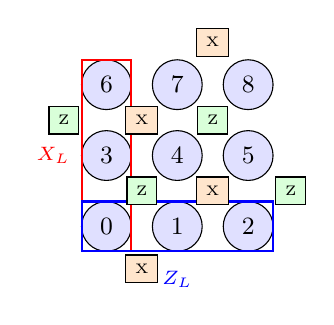
\begin{tikzpicture}[font=\small, scale=0.9]
    \foreach \id/\c/\r in {0/0/0,1/1/0,2/2/0,3/0/1,4/1/1,5/2/1,6/0/2,7/1/2,8/2/2}{
      \node[circle,draw,fill=blue!12,minimum size=18pt,inner sep=0pt] at (\c,\r) {\id};
    }
    \draw[thick,red] (-0.35,-0.35) rectangle (0.35,2.35);
    \node[red] at (-0.75,1) {\scriptsize $X_L$};
    \draw[thick,blue] (-0.35,-0.35) rectangle (2.35,0.35);
    \node[blue] at (1,-0.75) {\scriptsize $Z_L$};
    \node[draw,fill=green!15] at (0.5,0.5) {\tiny Z};
    \node[draw,fill=orange!20] at (1.5,0.5) {\tiny X};
    \node[draw,fill=orange!20] at (0.5,1.5) {\tiny X};
    \node[draw,fill=green!15] at (1.5,1.5) {\tiny Z};
    \node[draw,fill=orange!20] at (0.5,-0.6) {\tiny X};
    \node[draw,fill=orange!20] at (1.5,2.6) {\tiny X};
    \node[draw,fill=green!15] at (-0.6,1.5) {\tiny Z};
    \node[draw,fill=green!15] at (2.6,0.5) {\tiny Z};
  \end{tikzpicture}
  \caption{$d=3$ rotated 表面符号パッチの市松配置。円はデータ量子ビット（ローカル id $=3r+c$）、正方形はスタビライザ（バルク重み4／境界重み2）。赤枠が $X_L$（左列 $\{0,3,6\}$）、青枠が $Z_L$（下行 $\{0,1,2\}$）。}
  \label{fig:d3_patch}
\end{figure}

\subsection{geom\_lattice\_surgery / mpp 内の列挙ロジック}

\codepath{src/stages/01_mpp/src/ftqc/surface_patch.py} は、上の幾何・境界規約で決まる独立な 8 個のスタビライザを \texttt{GEOM\_STABS\_D3} という定数リストとして直接持っています。

\begin{lstlisting}[caption={$d=3$ パッチのスタビライザ列挙（\codepath{src/stages/01_mpp/src/ftqc/surface_patch.py}）},label=lst:geom_stabs_d3]
GEOM_STABS_D3 = [
    ("X", [0, 1]),       ("Z", [0, 1, 3, 4]),
    ("X", [1, 2, 4, 5]), ("Z", [2, 5]),
    ("Z", [3, 6]),       ("X", [3, 4, 6, 7]),
    ("Z", [4, 5, 7, 8]), ("X", [7, 8]),
]
\end{lstlisting}

同じファイルの \texttt{SurfacePatch} クラスは、この静的なリストを\textbf{自明に信用せず}、Stim 組み込みの \texttt{surface\_code:rotated\_memory\_z} 回路（アンシラベース、まだこの章では踏み込みません）を生成し、その \texttt{CX} スケジュールから逆に「どのアンシラがどのデータ集合を測っているか」を \texttt{\_extract\_stabilizers} で復元して、\texttt{GEOM\_STABS\_D3} と一致することを検証しています。
本章で必要なのは、幾何的な列挙（市松＋境界規則）と Stim の実装が一致しているという\textbf{事実}だけで、アンシラ側の \texttt{CX} スケジュールの詳細（第14–15章の主題）ではありません。
実際に確認すると、\texttt{SurfacePatch(3).stabilizers} は \texttt{GEOM\_STABS\_D3} と要素ごとに一致します。

\section{論理 \texorpdfstring{$X_L$・$Z_L$}{X\_L・Z\_L} とデータ/アンシラ}\label{sec:logical_ops}

\subsection{論理演算子の代表元}

$X_L$・$Z_L$ は、いずれのスタビライザとも可換でありながらスタビライザ群には含まれない演算子、すなわちパウリ群内の中心化群（慣例的には正規化群）の剰余類の代表元として選びます\cite{gottesman1997stabilizer}。
\texttt{SurfacePatch} では、図~\ref{fig:d3_patch} の左列を $X_L$、下行を $Z_L$ の代表元に採っています。

\begin{lstlisting}[caption={論理演算子の支持集合（\codepath{src/stages/01_mpp/src/ftqc/surface_patch.py} の \texttt{SurfacePatch.\_\_init\_\_}）},label=lst:xl_zl]
# 論理演算子: XL=左列(x=1), ZL=下行(y=1)
self.XL = sorted(self.stim2local[q] for q, c in self.data.items() if c[0] == 1)
self.ZL = sorted(self.stim2local[q] for q, c in self.data.items() if c[1] == 1)
\end{lstlisting}

これにより \texttt{XL == [0, 3, 6]}、\texttt{ZL == [0, 1, 2]} となり、いずれも重み $3=d$ の一列（一行）です。
重みが符号距離 $d$ に一致するのは偶然ではなく、$d$ とは「ある論理状態を別の論理状態へ変える最小の誤りの個数」（第3章）そのものだからです。
左列の $X$ 鎖は $X_L$、下行の $Z$ 鎖は $Z_L$ を実装し、全スタビライザと可換なまま相補的な論理値を反転します。$Y$ 鎖は $X$ 成分と $Z$ 成分を同時に持つため、任意の列へ置いたものが同じ性質を持つとは限りません。

\subsection{メモリの向き}

本章で使うメモリ実験は\textbf{$Z$ 基底メモリ}です。
データ量子ビットを $\ket{0}^{\otimes 9}$（$Z$ 固有状態）に初期化し、スタビライザ測定を何ラウンドか繰り返した後、最終的に $Z_L$ を読み出します。
この向きが重要なのは、初期状態が $Z$ 固有状態であるために\textbf{ラウンド0では $Z$ 型スタビライザだけが決定論的}になり、$X$ 型スタビライザは初期化直後には値が定まっていない、という非対称性が生じる点です（次節の検出器則に直結します）。
これは Stim 側のタスク名 \texttt{surface\_code:rotated\_memory\_z} の「\texttt{\_z}」が指す向きと同じです。
逆向きの $X$ 基底メモリも同じ幾何で対称的に作れますが、本章の中心である \texttt{mpp\_memory\_logical\_error}（次節）は $Z$ 基底メモリのみをハードコードしています。これは意図的な単純化であり、$X$ 基底版は同じ考え方を左右対称に適用すれば作れます。

\subsection{データ量子ビットだけで構成する理由}

第3章で確認したとおり、シンドローム測定は本来\textbf{アンシラを介した間接測定}です。
しかし MPP を使う本章の構成には、物理的なアンシラ量子ビットが 1 個も現れません。
これは MPP が「複数データ量子ビットにまたがる多体パウリ演算子を、Stim の内部でアンシラなしに直接測定する」という\textbf{理想化された命令}だからです。
実機ではこの多体測定を、補助量子ビットと \texttt{CX} 列で段階的に構成する必要があります（第14章以降）。
本章では、その配線の詳細をいったん脇に置き、「どの多体パウリをいつ測るか」という幾何とロジックだけを先に固めます。

\section{スタビライザ測定とノイズ（MPP）}\label{sec:mpp_noise}

\subsection{MPP の意味（現象論）}

Stim の \texttt{MPP} 命令は、\texttt{stim.target\_x}／\texttt{target\_z} と \texttt{stim.target\_combiner()} を組み合わせることで、互いに可換な多体パウリ積を測定命令として指定できます\cite{gidney2021stim,stim2026python}。
\codepath{src/stages/01_mpp/src/ftqc/surface_patch.py} の \texttt{mpp\_memory\_logical\_error} は、この命令を使って \texttt{GEOM\_STABS\_D3} の 8 個のスタビライザを毎ラウンド直接測定します。

\begin{lstlisting}[caption={MPP によるスタビライザ測定（\codepath{src/stages/01_mpp/src/ftqc/surface_patch.py} の \texttt{mpp\_memory\_logical\_error} を抜粋）},label=lst:mpp_measure]
for rnd in range(rounds + 1):
    c.append("DEPOLARIZE1", data, p)          # データ量子ビットの脱分極誤り
    for si, (t, sup) in enumerate(sp.stabilizers):
        tg, first = [], True
        fn = {"X": stim.target_x, "Z": stim.target_z}
        for q in sup:
            if not first:
                tg.append(stim.target_combiner())
            tg.append(fn[t](q))
            first = False
        c.append("MPP", tg, p)                # 多体パウリ測定自体にも誤り率 p
\end{lstlisting}

ここでノイズは 2 か所に入っています。
\texttt{DEPOLARIZE1(data, p)} はラウンドごとにデータ量子ビットが受ける物理誤りで、これは第3章の「反復符号でビットが確率 $p$ で反転する」に対応する現象論的ノイズです。
一方 \texttt{MPP(tg, p)} の第 2 引数 \texttt{p} は、測定そのものが確率 $p$ で誤った結果を返すという抽象化で、アンシラ経由の測定で本来起きる測定誤り・伝播誤りをひとまとめに近似したものです。
これは Stim が提供する現象論ノイズモデルの標準的な使い方であり、実際のゲート単位の誤り伝播（第14章以降の回路レベルノイズ）とは異なる、より粗い近似であることを明示しておきます。

\subsection{一様検出器則の導入}

アンシラを使わない MPP では、同じスタビライザを毎ラウンド同じ添字 \texttt{si} で測り続けるため、検出器則は非常に単純になります。
「同じ添字のスタビライザを、直前ラウンドの測定値と比較する」という\textbf{一様規則}だけで済みます。

\begin{lstlisting}[caption={一様検出器則（\codepath{src/stages/01_mpp/src/ftqc/surface_patch.py} の \texttt{mpp\_memory\_logical\_error} を抜粋）},label=lst:uniform_detector]
if si in prev:
    dets.append([mc, prev[si]])   # 直前ラウンドの同じスタビライザと比較
elif t == "Z":
    dets.append([mc])            # ラウンド0は Z 型のみ単独で決定論的
prev[si] = mc
\end{lstlisting}

ラウンド 0 では、初期状態が $Z$ 固有状態であるために $Z$ 型スタビライザだけが単独で決定論的検出器になり、$X$ 型スタビライザは「まだ比較対象がない」ので検出器を張りません。
ラウンド 1 以降はすべてのスタビライザについて「今回の値 XOR 前回の値」を検出器にします。
最後に $Z_L$ を直接 \texttt{MPP} で測定し、観測量として登録します。
このシンプルさは MPP という理想化の恩恵であり、アンシラ回路ではスタビライザの支持集合自体は変わらなくても、測定順序に依存した\textbf{フック誤り}が絡んでくるため、検出器則の導出はもう一段階複雑になります（第14–15章）。

\section{メモリ実験と論理エラー率}\label{sec:memory_exp}

\subsection{shots}

\codeinline{mpp_memory_logical_error(p, rounds=3, shots=40000)} は、上記の回路を \codeinline{compile_detector_sampler().sample(shots, separate_observables=True)} で多数回サンプリングし、\texttt{pymatching.Matching} でデコードした予測と実際の観測量との XOR の平均を論理エラー率として返します。
\texttt{shots} を増やすほどモンテカルロ推定の統計誤差が小さくなります。真の論理エラー率を $p_L$、ショット数を $N$ とすると、標本比率の標準誤差はおおよそ $\sqrt{p_L(1-p_L)/N}$ です。したがって 4 万 shots が与える桁数は $p_L$ に依存し、失敗が0件でも誤り率が0と確定するわけではなく、95\% 上限の目安は $3/N$ です。

\begin{lstlisting}[caption={メモリ実験の最小実行例},label=lst:memory_min]
# src/stages/01\_mpp で `uv run` して実行する
from ftqc.surface_patch import mpp_memory_logical_error

for p in (0.0, 0.001, 0.003, 0.005, 0.01):
    err = mpp_memory_logical_error(p, rounds=3, shots=40000)
    print(f"p={p:<6} logical_error_rate={err:.4f}")
\end{lstlisting}

\subsection{$p$ 依存の直感}

上の例を実行すると、おおむね次のような結果が得られます（乱数依存のため実行毎に数値は変動します）。

\begin{lstlisting}[caption={実行例の出力},label=lst:memory_output]
p=0.0    logical_error_rate=0.0000
p=0.001  logical_error_rate=0.0027
p=0.003  logical_error_rate=0.0058
p=0.005  logical_error_rate=0.0125
p=0.01   logical_error_rate=0.0256
\end{lstlisting}

$p=0$ ではこの実行例の観測失敗率が $0$ になり、$p$ を大きくすると期待される論理エラー率は増加する傾向を示します。有限ショットの各推定値は統計揺らぎを持つため、個々の実行結果が厳密に単調になる保証はありません。
第3章・第4章で定式化したとおり、量子符号距離 $d$（非自明な論理演算子の最小重み）に対して、重み $d-1$ 以下の Pauli 誤りはシンドロームを生じるかスタビライザとして自明に作用し、重み $t = \lfloor (d-1)/2 \rfloor$ 以下の任意の Pauli 誤りを訂正できます。
本章でのシミュレーション（\texttt{mpp\_memory\_logical\_error}）は、ランダムに注入される物理誤りに対する論理エラー率の単調性やデコーダの全体的な応答挙動を確認するものであり、個々の誤りに対する訂正半径 $t$ を直接検証する実験ではない点に注意してください。
本章の段階では、この単調性を現象論レベルで確認するだけにとどめます。
物理誤り率としきい値 $p_{\mathrm{th}}$ の関係、符号距離 $d$ を増やしたときのスケーリングといった定量的な議論は、合否基準を厳密に定義する第8章以降の主題です。

\codepath{src/stages/01_mpp/src/ftqc/surface_patch.py} の \texttt{demo()} は、この MPP 版（アンシラなし・直接測定）と、Stim 組み込みのアンシラベース回路（\texttt{SurfacePatch.memory\_circuit} / \texttt{decode}、ともに回路レベル）を同じ $p$ で比較しています。
この実装例では、同じ数値 $p$ でも回路レベル版の方が論理エラー率が高くなる傾向があります。ただし両モデルでは $p$ が付く誤り位置とチャネルの数が異なるため、同じ $p$ は同じ総ノイズ強度を意味しません。この比較は、回路レベル版だけが \texttt{CX} や測定を介する伝播（フック誤り）を表せることを示す定性的な例です\cite{dennis2002topological,fowler2012surface}。

\section{やること・スコープ外}\label{ch7:scope}

\subsection{やること}

\begin{itemize}
  \item 市松配置と境界規則にもとづく $d=3$ パッチのスタビライザ列挙（\texttt{GEOM\_STABS\_D3}、\texttt{SurfacePatch.stabilizers}）。
  \item データ量子ビットの支持集合としての論理演算子 $X_L$・$Z_L$ の定義。
  \item MPP によるアンシラなしのスタビライザ測定と、一様検出器則の導入。
  \item $Z$ 基底メモリ実験の実装と、$p$ に対する論理エラー率の単調な増加傾向の現象論的な確認。
\end{itemize}

\subsection{スコープ外}

\begin{itemize}
  \item アンシラベースの \texttt{CX} スケジュール設計そのもの。本章では \texttt{SurfacePatch} が内部検証のために Stim 組み込み回路を使う場面にだけ触れ、スケジュールの中身には踏み込みません（第14–15章）。
  \item 回路レベルノイズにおける符号距離の厳密な議論（\texttt{shortest\_graphlike\_error} による検証）。本章で確認するのは「ノイズなしで検出器が決定論的になる」という、より弱い条件だけです。
  \item $X$ 基底メモリ実験、複数パッチの格子手術（第9–11章）。
\end{itemize}

\section{合否基準での検証}\label{ch7:verification}

本書全体の合否基準には、\codepath{tests/} や \texttt{ls\_handoff\_shells.py} が実践する次の 2 点があります：本書の非 gauge 回路について検出器が決定論的であること、未分解 DEM の全誤り機構が graphlike などの条件を満たす場合に\textbf{\texttt{shortest\_graphlike\_error} が意図した距離 $d$ に一致}すること。
これらの厳密な定義と検証手順は第8章でまとめて導入します。

本章の段階（Stage 01 入口）でサンプリングにより確認できるのは、$p=0$ で観測した範囲に検出器反転と論理失敗がないという統計的な健全性です。
第7.4節の最小実行例で $p=0$ の標本論理エラー率が $0$ になることだけでは、全検出器・観測量の決定論性の証明にはなりません。厳密な確認には Stim の tableau 解析を用いる DEM 構築などが必要です\cite{gidney2021stim,stim2026python}。
一方 \texttt{shortest\_graphlike\_error} による距離の厳密な検証は、検出器誤りモデル（DEM）を明示的に構築して初めて意味を持つため、その手続きと合否用語の正式な定義は次章に委ねます。

\section{まとめ}\label{ch7:summary}

\begin{itemize}
  \item 本章の $d=3$ rotated 表面符号パッチは、採用した市松配置と境界規約によって重み 4（バルク）・重み 2（境界）の独立なスタビライザ 8 個として列挙されます。
  \item 論理演算子 $X_L$・$Z_L$ は、それぞれ左列・下行というデータ量子ビットの支持集合で代表され、その重みは符号距離 $d$ に一致します。
  \item MPP はアンシラを使わずに多体パウリ演算子を直接測定する理想化であり、スタビライザの幾何と検出器則だけに集中するための現象論的な近似です。
  \item MPP では「同じスタビライザを直前ラウンドと比較する」一様検出器則だけでメモリ実験が組めますが、これはアンシラ回路のフック誤りを無視した楽観的な近似でもあります。
  \item $Z$ 基底メモリ実験では、$p=0$ の標本失敗率が0であることと、$p$ に対する論理エラー率の増加傾向を確認できます。有限ショット結果は統計揺らぎを持ちます。
\end{itemize}

次章では、本章で仮置きにした「決定論性」と「距離」を、\texttt{shortest\_graphlike\_error} や gauge 検出器ゼロという機械的に検証可能な合否基準として正式に定義し、MWPM や BP+OSD によるデコードと結び付けます。

\begin{exercise}
  \begin{enumerate}
    \item 図~\ref{fig:d3_patch} を参考に、ローカル id $4$（中心のデータ量子ビット）が支持集合に含まれるスタビライザをすべて列挙し、その型と重みを答えなさい。
    \item $X_L=\{0,3,6\}$ に $Z$ 誤りを 1 個だけ作用させたとき、\texttt{GEOM\_STABS\_D3} のうちどのスタビライザの測定値が反転するかを求め、その位置から誤りが起きたデータ量子ビットを一意に特定できるかどうかを議論しなさい。
    \item \texttt{mpp\_memory\_logical\_error} の \texttt{DEPOLARIZE1(data, p)} の行を削除（$p=0$ に固定）した場合と、\texttt{MPP(tg, p)} の第 2 引数だけを $0$ にした場合とで、それぞれ論理エラー率がどう変化すると予想されるかを、本章のノイズモデルの説明にもとづいて答えなさい。
    \item 本章の $Z$ 基底メモリ実験を $X$ 基底に変更するには、\texttt{mpp\_memory\_logical\_error} のどの箇所（初期化・検出器則・最終観測量）をどのように書き換える必要があるか、$X_L$・$Z_L$ の対称性にもとづいて説明しなさい。
  \end{enumerate}
\end{exercise}

% Stage: 01 入口 ／ 説明用コード: src/stages/01\_mpp/src/ftqc（基準は advanced 整合）
\chapter{デコードと評価の基準}\label{ch:decoding}

\begin{chaptergoal}
  \begin{itemize}
  \item ノイズモデルの階層（現象論モデルと回路レベルモデルの違い）を整理します。
  \item MWPM（最小重み完全マッチング）による復号の考え方と PyMatching（対象バージョン 2.4.0）の使いかたを理解します\cite{higgott2022pymatching,higgott2025sparse}。
  \item 本書全体を通じて使う合否基準——gauge 検出器ゼロ、厳密条件を満たす場合の回路距離（それ以外は graphlike／探索上界）、真理値表・理想分布一致、seed 再現性、\texttt{allow\_gauge\_detectors} を使わない——を確定します。
  \item graphlike ではない検出器誤りモデルに対する BP+OSD フォールバックの位置づけを理解します。
  \end{itemize}
\end{chaptergoal}

前章までで、Stim の DETECTOR・OBSERVABLE\_INCLUDE の基本（第6章）と、MPP によるパッチ構築（第7章）に触れました。
ここまでの実装は、いずれも「回路を作って測定すれば、それでよい」という段階にとどまっています。
しかし本書の目的はシミュレータを\textbf{作ること}であって、作ったつもりのコードが本当に量子誤り訂正として機能しているかは別問題です。
検出器の作り方を一つ間違えても Stim はエラーを出さずに走り続けますし、符号距離を意図せず落としてしまうバグも黙って通り抜けます。

本章では、この「作ったつもりのコード」に対して機械的に白黒をつけるための\textbf{合否基準}を定義します。
以降の各章は、新しい構成要素（トランスバーサル操作や格子手術など）を導入するたびに、ここで定義する基準に照らして「本当に機能しているか」を検証します。
つまり本章は、個々の技術の説明ではなく、本書全体の「ものさし」を作る章です。

\begin{notebox}
  Stage: \textbf{01}。
  説明用コードは主に \codepath{src/stages/01_mpp/src/ftqc/} を用いますが、合否基準の語彙と最終形は \codepath{tests/} と公開版の実装に整合させます。
  Stage 01 の時点ではまだ測れない項目（たとえば \texttt{decode\_shell} の seed 対応）もあり、その点は本章で明示します。
\end{notebox}

\section{ノイズモデルの階層}\label{sec:noise_models}

\subsection{現象論モデルと回路レベルモデル}

量子誤り訂正の数値実験でノイズを入れる方法には、大きく 2 つの階層があります。

\begin{itemize}
  \item \textbf{現象論モデル}：各ラウンドでデータ誤りとシンドローム測定誤りを直接確率的に与え、測定回路の内部構造を理想化します。文献や実装によってチャネルの細部は異なりますが、測定値反転だけを指す語ではありません。アンシラを介した CNOT の順序を再現しないため、測定回路自身の誤り伝播（後述の hook 誤り）は表現できません\cite{dennis2002topological}。
  \item \textbf{回路レベルモデル}：実際の物理ゲート列（初期化・CNOT・測定）に対して \texttt{DEPOLARIZE1}／\texttt{DEPOLARIZE2}／測定前フリップなどのノイズを 1 ゲートごとに挿入し、シンドローム測定回路そのものの誤り伝播を再現します。
\end{itemize}

第III部（Stage 01）では、\codepath{src/stages/01_mpp/src/ftqc/} のコードは主に MPP（多体パウリ測定）でスタビライザを直接測定する現象論に近いモデルを使います。
一方で、本書の合否基準そのものは Stim の \texttt{stim.Circuit.generated} が提供する回路レベルの表面符号回路でも検証できます。
例として \codepath{src/stages/01_mpp/src/ftqc/ftqc_toy.py} の STAGE 1 は、回路レベルノイズを持つ \texttt{surface\_code:rotated\_memory\_z} を直接組み立てています。

\begin{lstlisting}[language=Python, caption={回路レベルノイズを持つ表面符号メモリ実験（src/stages/01\_mpp/src/ftqc/ftqc\_toy.py）}]
circuit = stim.Circuit.generated(
    "surface_code:rotated_memory_z",
    distance=distance,
    rounds=rounds,
    after_clifford_depolarization=p,      # 各 Clifford ゲート後の脱分極
    before_measure_flip_probability=p,    # 測定エラー
)
sampler = circuit.compile_detector_sampler()
det, obs = sampler.sample(num_shots, separate_observables=True)
dem = circuit.detector_error_model(decompose_errors=True)
matcher = pymatching.Matching.from_detector_error_model(dem)
pred = matcher.decode_batch(det)
n_err = int(np.sum(obs ^ pred))
\end{lstlisting}

\texttt{after\_clifford\_depolarization} は生成回路中の各 Clifford ゲート後に、ゲートの量子ビット数に応じた脱分極チャネルを挿入し、\texttt{before\_measure\_flip\_probability} は測定直前に結果を反転し得る誤りを挿入します\cite{stim2026python}。
これに対し、\codepath{src/stages/01_mpp/src/ftqc/geom_lattice_surgery.py} や \codepath{src/stages/02_circuit_level/src/ftqc/circuit_level_merge.py} のように、データ量子ビットとアンシラの両方に \texttt{DEPOLARIZE1}／\texttt{DEPOLARIZE2} を明示的に付ける実装もあり、現象論と回路レベルの境界は「アンシラを介した測定回路の各ゲートを陽に書くかどうか」で判断できます。

\begin{notebox}
  第14章「なぜ回路レベルが必要か」では、この 2 つの階層の差が\textbf{符号距離そのものに影響する}こと（hook 誤りによって回路レベル距離が符号距離を下回り得ること）を具体的に扱います。
  本章では、その差を検出するための道具（本節後半の $\mathrm{shortest\_graphlike\_error}$）を先に定義しておきます。
\end{notebox}

\subsection{DETECTOR と検出器誤りモデル}

Stim は回路中の物理誤りチャネルを伝播させてサンプルを生成でき、解析時にはその効果を DETECTOR（測定記録のパリティから作る 0/1 の量）と論理観測量の反転へ写します。
回路に対して \texttt{circuit.detector\_error\_model()} を呼ぶと、独立とみなす各誤り機構の確率、その検出器症状、論理フレーム変化を記録した\textbf{検出器誤りモデル}（DEM: Detector Error Model）が得られます\cite{gidney2021stim,stim2026doc}。
復号（デコード）とは、観測した検出器パターンから論理フレーム変化または訂正を推定する作業です。MWPM は graphlike 模型上で整合する辺集合の重みを最小化しますが、相関・縮退を含む一般模型の厳密な最尤誤り集合を必ず返すわけではありません\cite{higgott2022pymatching,higgott2025sparse}。

\section{MWPM による復号}\label{sec:mwpm}

\subsection{graphlike な誤りとマッチング}

DEM に現れる各誤り機構が反転させる検出器を高々 2 個持つとき、この DEM は\textbf{graphlike}であるといいます。0個は検出器症状のない論理誤り、1個は境界へ至る辺、2個は検出器間の辺に対応し、論理 observable target はこの個数に数えません\cite{stim2026doc}。
graphlike な DEM は、検出器を頂点、誤り機構を辺とするグラフとして表現できます。
反転した検出器（シンドローム）は、このグラフ上で「奇数個の端点を持つ頂点集合」として現れるので、復号問題は「シンドローム頂点どうしを辺のコストが最小になるように対にする」という\textbf{最小重み完全マッチング}（MWPM: Minimum Weight Perfect Matching）に帰着します。
本書では、この MWPM を高速に解くライブラリとして PyMatching を使います。
このマッチンググラフと復号の様子を図\ref{fig:ch8_matching_graph}に示します。

\begin{figure}[htbp]
  \centering
  \begin{tikzpicture}[
    detnode/.style={circle, draw=black!70, fill=white, thick, minimum size=16pt, inner sep=0pt, font=\footnotesize},
    defectnode/.style={circle, draw=red!70!black, fill=red!70!black, text=white, thick, minimum size=16pt, inner sep=0pt, font=\footnotesize\bfseries},
    boundnode/.style={rectangle, draw=black!60, fill=black!8, rounded corners=3pt, thick, minimum width=22pt, minimum height=64pt, align=center, font=\footnotesize},
    erredge/.style={draw=black!30, thick},
    matchedge/.style={draw=red!70!black, line width=2.4pt},
  ]
    % 境界ノード
    \node[boundnode] (BL) at (-0.5, 1.0) {境\\界};
    \node[boundnode] (BR) at (6.5, 1.0) {境\\界};

    % 検出器ノードグリッド (2行 x 3列)
    % 行1 (y=2.0)
    \node[detnode] (d11) at (1.2, 2.0) {$d_1$};
    \node[defectnode] (d12) at (3.0, 2.0) {$d_2$};
    \node[detnode] (d13) at (4.8, 2.0) {$d_3$};

    % 行2 (y=0.0)
    \node[detnode] (d21) at (1.2, 0.0) {$d_4$};
    \node[defectnode] (d22) at (3.0, 0.0) {$d_5$};
    \node[defectnode] (d23) at (4.8, 0.0) {$d_6$};

    % 通常エッジ (潜在的な誤り機構)
    \draw[erredge] (BL.north east) -- (d11);
    \draw[erredge] (BL.south east) -- (d21);
    \draw[erredge] (d11) -- (d12);
    \draw[erredge] (d12) -- (d13);
    \draw[erredge] (d13) -- (BR.north west);
    \draw[erredge] (d21) -- (d22);
    \draw[erredge] (d22) -- (d23);
    \draw[erredge] (d11) -- (d21);
    \draw[erredge] (d13) -- (d23);

    % マッチングエッジ（太線ハイライト）
    % d12 と d22 のマッチング
    \draw[matchedge] (d12) -- node[right=4pt, text=red!70!black, font=\footnotesize] {対消滅} (d22);
    % d23 と BR のマッチング（境界へ抜ける誤り鎖）
    \draw[matchedge] (d23) -- node[below=3pt, text=red!70!black, font=\footnotesize] {境界へ結合} (BR.south west);

    % 凡例 (Legend)
    \begin{scope}[shift={(0.0, -1.2)}]
      \node[detnode, minimum size=11pt] at (0.2, 0) {};
      \node[right, font=\footnotesize] at (0.45, 0) {未反応の検出器 ($0$)};

      \node[defectnode, minimum size=11pt] at (3.5, 0) {};
      \node[right, font=\footnotesize] at (3.75, 0) {反応した検出器 ($1$, フラストレーション)};
    \end{scope}
    \begin{scope}[shift={(0.0, -1.75)}]
      \draw[erredge] (0.2, 0) -- (0.7, 0);
      \node[right, font=\footnotesize] at (0.8, 0) {graphlike 誤り枝};

      \draw[matchedge] (3.3, 0) -- (3.8, 0);
      \node[right, font=\footnotesize] at (3.9, 0) {MWPM によるマッチング};
    \end{scope}

  \end{tikzpicture}
  \caption{MWPM によるマッチンググラフの概念図。検出器をノード、反転確率に応じた重みを持つ graphlike な誤り機構をエッジとして表します。シンドロームとして反応した検出器（塗りつぶしノード）のペアを最小コストで結ぶほか、表面符号の境界へ抜ける誤り鎖は境界ノード（Boundary）とマッチングさせることで完全マッチングを実現します。}
  \label{fig:ch8_matching_graph}
\end{figure}

\begin{lstlisting}[language=Python, caption={PyMatching による MWPM 復号（src/stages/02\_circuit\_level/src/ftqc/circuit\_level\_merge.py）}]
def decode(self, c, shots=40000):
    det, obs = c.compile_detector_sampler().sample(shots, separate_observables=True)
    try:
        dem = c.detector_error_model(decompose_errors=True)
        m = pymatching.Matching.from_detector_error_model(dem)
        pred = m.decode_batch(det)
        which = "MWPM"
    except ValueError:
        from stimbposd import BPOSD
        pred = BPOSD(c.detector_error_model(decompose_errors=False), max_bp_iters=40).decode_batch(det)
        which = "BP+OSD"
    return (obs ^ pred).mean(axis=0), which
\end{lstlisting}

\texttt{decompose\_errors=True} を付けると、Stim は 3 個以上の検出器を同時に反転させる誤り機構について、区切り記号で関連づけた graphlike 成分への分解を提案します。分解不能なら既定では DEM 構築が失敗し、分解後の成分を独立辺として MWPM へ渡すと元の相関を近似または失う場合があります\cite{stim2026doc}。
掲載コードの \texttt{except ValueError} は実装上のフォールバックですが、\texttt{ValueError} は非 graphlike 以外の入力不備でも起こり得ます。堅牢な実装では未分解 DEM の構造と例外内容を確認して分岐する必要があります。
このフォールバックの受け皿が、8.4 節で扱う BP+OSD です。

\subsection{符号距離とデコーダ観測量の関係}

第3章・第4章で導入した符号距離 $d$ は、「ある論理状態を別の論理状態に変えてしまう最小の誤りの個数」でした。
すべての誤り機構が graphlike な回路に対しては、Stim はこれを計算する手段を提供しています。

\begin{lstlisting}[language=Python, caption={shortest\_graphlike\_error による graphlike 上界の確認（src/stages/02\_circuit\_level/src/ftqc/circuit\_level\_merge.py）}]
cdist, _, _ = clm.build(aone=True, noise=True, p=0.005)
bound = len(cdist.shortest_graphlike_error(ignore_ungraphlike_errors=True))
print(f"DEM 上の最短 graphlike 論理誤り = {bound} (回路距離の上界)")
\end{lstlisting}

\texttt{circuit.shortest\_graphlike\_error()} は、その回路から得た DEM 上で、検出器症状を残さず論理観測量を反転させる graphlike 誤り機構の組み合わせのうち、機構数が最小のものを返します。確率の大小は目的関数に使いません\cite{stim2026python}。
ただし、Stim では既定値が \texttt{ignore\_ungraphlike\_errors=True} であり、非 graphlike 誤り（検出器 3 個以上を発火させる誤りや分解不能な誤り）は自動的に無視されます。そのため、単に引数なしで呼び出した場合に返される長さは、一般には真の回路距離の\textbf{上界（upper bound）}に過ぎません。

これが厳密な\textbf{回路レベルの距離}（\texttt{graphlike\_exact}）と呼べるのは、未分解 DEM の各物理誤り機構が検出器を高々 2 個しか反転しないことを先に確認し、\texttt{ignore\_ungraphlike\_errors=False} を指定した探索が成功し、返された各項に実際の回路誤りが対応している場合に限られます。単に「高次誤りを graphlike 成分へ分解できた」だけでは、成分数と物理 fault 数が一致しないため、この条件を満たしません。
これが設計上意図した符号距離 $d$（たとえばパッチ距離 3 の表面符号なら $d=3$）と一致するかどうかは、本章で定義する合否基準の中心をなします。
一致していなければ、検出器の張り方や測定順序のどこかに、距離を落としてしまうバグ（第14章で扱う hook 誤りなど）が潜んでいる、ということになります。

\section{本書の合否基準}\label{sec:criteria}

以上を踏まえて、本書のシミュレータが新しい構成要素（ゲート・符号・格子手術・スケジュールなど）を追加するたびに満たすべき合否基準を、以下の 5 項目として確定します。
用語と最終的な定義は \codepath{tests/} と公開版に含む tests/ とコードに整合させています。

\begin{enumerate}
  \item \textbf{本書の非 gauge 回路で検出器が決定論的}：\texttt{noise=False} の回路について、既定の \texttt{allow\_gauge\_detectors=False} で DEM 構築が成功することを主判定とします。有限回サンプリングで反転がないことは補助的な健全性確認であり、決定論性の証明ではありません。
    \codepath{src/ftqc/ls_cnot_ft.py} の \texttt{demo()} は、この点を次のように直接検査しています。
\begin{lstlisting}[language=Python, caption={gauge 検出器ゼロの検査（src/ftqc/ls\_cnot\_ft.py）}]
c0, _, _ = g.build(noise=False)
det, _ = c0.compile_detector_sampler().sample(3000, separate_observables=True)
nd = int(det.any(axis=0).sum())
print(f"検出器数={c0.num_detectors}, 非決定論的={nd}  "
      f"({'OK — allow_gauge_detectors 不要' if nd == 0 else 'NG'})")
\end{lstlisting}
    \texttt{det.any(axis=0).sum()} は「標本内で一度でも 1 になった検出器の個数」を数えます。本書の通常のスタビライザ回路でノイズなしの検出器が揺れるならバグの兆候です。一方、subsystem code などでは gauge detector を意図的に使う場合があり、非決定論的検出器が一般に誤りとは限りません\cite{stim2026python}。

  \item \textbf{未分解の全誤り機構が graphlike なら $\mathrm{shortest\_graphlike\_error}=d$}：前節で見た事前検査を満たし、\texttt{ignore\_ungraphlike\_errors=False} で求めた \texttt{circuit.shortest\_graphlike\_error()} の長さが、設計上の符号距離 $d$ に一致すること（非 graphlike な DEM の場合は \texttt{search\_for\_undetectable\_logical\_errors} 等による探索上界として扱います）。
    回路から graphlike 上界を得る基本形は次のとおりです。
\begin{lstlisting}[language=Python, caption={回路距離の graphlike 上界（Stim Circuit API）}]
noisy.detector_error_model(decompose_errors=True,
                           allow_gauge_detectors=False)
bound = len(noisy.shortest_graphlike_error(ignore_ungraphlike_errors=True))
print(f"graphlike upper bound={bound}")
\end{lstlisting}
    \texttt{method == "graphlike\_exact"} の場合にだけ \texttt{value} を厳密距離と呼びます。\texttt{"graphlike\_upper\_bound"} や \texttt{"search\_upper\_bound"} の場合は、意図した距離と整合する証拠にはなりますが、距離保存の証明にはなりません。
    非 graphlike な回路（本書では対象外の高重み検査回路など）では厳密値が計算できないため、この基準は 8.4 節で述べる探索上界に置き換わります。

  \item \textbf{選んだ入力・測定設定で理想結果と一致}：計算基底入力に対する論理演算（CNOT など）の出力が、期待される古典的な真理値表と一致すること。
    たとえば \codepath{src/ftqc/ls_cnot_ft.py} の \texttt{demo()} は、制御・標的の 4 通りの入力それぞれについて $(c,t)\to(c,\,c\oplus t)$ を確認しています。
    計算基底の真理値表だけでは相対位相を検査できません。重ね合わせ入力や複数の測定基底を加え、Qulacs による理想分布との TVD なども使います。ただし有限個の設定と有限ショットによる一致は、量子チャネル全体の等価性の証明ではありません。

  \item \textbf{seed 再現性}：再現可能なサンプリング経路では、同じ \texttt{seed} から同じシンドロームと復号結果が得られることを確認します。現行 Stage 03 の \texttt{decode\_shell(shell, shots=...)} は seed 引数を受けず、runtime 内の Stim detector sampler 呼び出しも seed を渡していません。したがって QEC sampling を含む runtime 全体の再現性は、この API では保証されません。公開テストの同一 seed 検査は \texttt{qec\_mode="off"} の実行経路を対象にしており、QEC sampling の再現性を検査するものではありません。

  \item \textbf{shell の gauge 方針}：本書の shell 契約では \texttt{allow\_gauge\_detectors} を使いません。Stim の \texttt{detector\_error\_model()} は、回路状態に対して非決定的な検出器があると既定でエラーを出します。このオプションは、互いに反可換な非決定的検出器を gauge として扱い、対応する確率 $1/2$ の機構を DEM に加える正規の機能です\cite{stim2026python}。
    本書のシェル構築コードは、この抑制オプションを\textbf{使いません}。
\begin{lstlisting}[language=Python, caption={allow\_gauge\_detectors を使わない方針（src/ftqc/ls\_handoff\_shells.py の decode\_shell docstring）}]
"""
Does NOT use allow_gauge_detectors.  All shells produced here are built so
that the noiseless circuit has zero non-deterministic detectors; if the DEM
build raises a "non-deterministic detector" error, that signals a malformed
shell (the gauge allowance would only hide the bug and collapse distance),
so the error is allowed to propagate as a correctness guard.
"""
\end{lstlisting}
    本書の shell は通常のスタビライザ回路として全検出器を決定論的に設計する契約なので、このオプションを使わず例外を伝播させます。この契約下では安易な指定が構築バグを隠し得ますが、オプション自体が一般に距離を崩すわけではありません。意図的な gauge 回路では、検出器の代数と距離の定義を別途定めて使用します。
\end{enumerate}

\begin{warningbox}
  第6章で触れた \texttt{allow\_gauge\_detectors} の落とし穴は、この項目 5 として本章で正式な合否基準になりました。
  本書の shell に「エラーが出て動かないから \texttt{allow\_gauge\_detectors=True} を付ける」という対処は\textbf{禁止}です。まず検出器の張り方・測定順序を見直します。意図的な subsystem/gauge 構成はこの shell 契約の対象外です。
\end{warningbox}

\subsection{Stage 01 における適用範囲}

Stage 01 と Stage 03 の公開スナップショットに含まれる \texttt{decode\_shell} は、いずれも sampler seed を受け取る引数を持ちません。

\begin{lstlisting}[language=Python, caption={Stage 01 の decode\_shell（src/stages/01\_mpp/src/ftqc/ls\_handoff\_shells.py）}]
def decode_shell(shell: ShellCircuit, shots: int = 1000) -> ShellDecodeResult:
    ...
    det, obs = circ.compile_detector_sampler().sample(shots, separate_observables=True)
\end{lstlisting}

このため項目 4 は望ましい検証基準として定義しますが、公開 runtime の QEC sampling に対しては未達です。Stage 01／02 の各デモが確認する範囲も、決定論性・距離条件・位相を含む機能同値性を一括して証明するものではありません。
本書では、各 Stage の実装が実際に満たす基準と、未達の基準を区別して記述します。

\section{BP+OSD フォールバック}\label{sec:bposd}

\subsection{非 graphlike な誤りモデル}

3 個以上の検出器を同時に反転させる誤り機構が \texttt{decompose\_errors=True} でも graphlike な成分に分解できない場合、その DEM は\textbf{非 graphlike}（ハイパーグラフ的）です。
このような DEM は、頂点と辺だけのグラフでは表現できず、MWPM の枠組みをそのまま適用できません。
8.2 節のコード例で見たとおり、本書の復号関数は \texttt{pymatching.Matching.from\_detector\_error\_model} が \texttt{ValueError} を投げたときに、この非 graphlike な場合の受け皿として BP+OSD（Belief Propagation + Ordered Statistics Decoding）へフォールバックします。

\begin{lstlisting}[language=Python, caption={BP+OSD フォールバック（再掲、src/stages/02\_circuit\_level/src/ftqc/circuit\_level\_merge.py）}]
try:
    dem = c.detector_error_model(decompose_errors=True)
    m = pymatching.Matching.from_detector_error_model(dem)
    pred = m.decode_batch(det)
    which = "MWPM"
except ValueError:
    from stimbposd import BPOSD
    pred = BPOSD(c.detector_error_model(decompose_errors=False), max_bp_iters=40).decode_batch(det)
    which = "BP+OSD"
\end{lstlisting}

BP+OSD は、まずビリーフプロパゲーションで誤り変数の周辺信頼度を反復的に推定し、BP が有効な解を返さない場合などに、その信頼度で列を並べ替えて情報集合を選び、低次数の候補を再処理する Ordered Statistics Decoding を組み合わせる復号法です\cite{roffe2020bposd}。
MWPM のようにグラフ上の最短距離問題に帰着できない一般のパリティ検査行列（qLDPC 符号など）に対しても適用できる代わりに、MWPM より計算コストが高く、厳密性（最小重みの保証）もありません。

\subsection{距離検証への影響と本書の報告範囲}

非 graphlike な回路では、8.3 節項目 2 の $\mathrm{shortest\_graphlike\_error}$ による厳密な距離計算はそのままでは使えません。
本書で採用する評価上の注意 が示す方針では、こうした場合に \texttt{stim.Circuit.search\_for\_undetectable\_logical\_errors} による\textbf{探索上界}を代替の距離証拠として用い、戻り値に \texttt{"search\_upper\_bound"} のような手法名を明記することで、厳密値と探索上界を区別して報告します。
本書では、未分解 DEM の各機構と1物理 fault の対応など前節の条件を満たす graphlike 回路には $\mathrm{shortest\_graphlike\_error}=d$ を厳密値として使います。それ以外では探索上界と、必要なら論理エラー率の $p$ 依存性を組み合わせた証拠を使い、厳密距離とは区別します。

本書では BP+OSD は、graphlike DEM を MWPM で扱えない場合のフォールバックとして紹介します。復号器が返す解は一般に最尤解の保証ではなく、回路の距離評価とも区別してください。

\section{やること・スコープ外}\label{sec:decoding_scope}

\subsection{やること}

\begin{itemize}
  \item ノイズモデルの階層（現象論／回路レベル）を整理し、両者の違いが符号距離に影響し得ることを予告する。
  \item MWPM による復号の仕組みと、graphlike という判定基準を PyMatching の実装レベルで示す。
  \item 本書全体で使う 5 項目の合否基準を確定し、Stage 01 の時点でどこまで検証できるかを明示する。
  \item BP+OSD フォールバックの役割と、graphlike 条件の制限を説明する。
\end{itemize}

\subsection{スコープ外}

\begin{itemize}
  \item hook 誤りの詳細な機構と、回路レベル距離が符号距離を下回る具体的な様子（第14章）。
  \item BP+OSD のビリーフプロパゲーションの数式的な詳細と収束性の議論（発展章で必要に応じて触れます）。
  \item 探索上界を計算する \texttt{search\_for\_undetectable\_logical\_errors} の詳細な探索パラメータ設計。
  \item 複数の判定結果を一つの汎用ユーティリティへ集約する設計。本書では各検査を対象コードとテストに即して説明します。
\end{itemize}

\section{まとめ}\label{ch8:summary}

\begin{itemize}
  \item ノイズには現象論モデルと回路レベルモデルの 2 階層があり、後者だけが測定回路自身の誤り伝播（hook 誤りなど）を再現できます。
  \item DEM が graphlike であれば、検出器を頂点とするグラフ上で MWPM を適用できます。これは graph model に対する最小重み解であり、一般の相関模型の厳密最尤復号と同義ではありません。
  \item 本書の合否基準は次の 5 項目です。
    \begin{enumerate}
      \item 本書の非 gauge 回路では既定設定で検出器が決定論的。
      \item 未分解 DEM の全機構が graphlike などの条件を満たす場合に限り、最短 graphlike 論理誤りの機構数を距離 $d$ と照合。
      \item 選んだ入力・測定設定で真理値表・理想分布と一致。
      \item seed 再現性。
      \item \texttt{decode\_shell} は \texttt{allow\_gauge\_detectors} を使ってバグを隠さない。
    \end{enumerate}
  \item 項目 4 は理想的な基準として示しますが、QEC sampling に seed を渡す API は本書の公開 snapshot には含まれていません。
  \item 本書の実装では非 graphlike な DEM に BP+OSD を使い、距離は探索上界で評価します。一般の非 graphlike 回路では、採用する復号器と評価手法を回路に応じて別途選ぶ必要があります。
\end{itemize}

次章では、この合否基準を実際の物差しとして使いながら、トランスバーサル操作と生成子追跡による Clifford の完全な誤り耐性化を扱います。

\begin{exercise}
  \begin{enumerate}
    \item \codepath{src/stages/02_circuit_level/src/ftqc/circuit_level_merge.py} の \texttt{demo()} 内で、「検出器の決定論性」（[C]）と「回路レベル距離」（[D]）をそれぞれ確認しているコードを引用し、それぞれが本章のどの合否基準項目に対応するかを説明しなさい。
    \item \texttt{allow\_gauge\_detectors=True} を使って non-deterministic detector エラーを抑制した場合に、本章の合否基準のどの項目が実質的に検証されなくなるかを、$\mathrm{shortest\_graphlike\_error}$ の計算方法に触れながら説明しなさい。
    \item \texttt{pymatching.Matching.from\_detector\_error\_model} が \texttt{ValueError} を投げる状況を、graphlike・非 graphlike という語を使って説明し、そのときに呼び出されるデコーダの名前を答えなさい。
    \item Stage 01 と公開 Stage 03 の \texttt{decode\_shell} の sampler 呼び出しを比較し、両者が seed 再現性の基準を満たすかを判断しなさい。
  \end{enumerate}
\end{exercise}

% ----- 第III部 -----
\part{Stage 01 — 現象論 MPP で論理演算まで}\label{part:stage_01}

% Stage: 01 ／ 説明用コード: src/stages/01\_mpp/src/ftqc
\chapter{トランスバーサル操作と生成子追跡}\label{ch:transversal}

\begin{chaptergoal}
  \begin{itemize}
  \item トランスバーサル操作がなぜ誤り耐性を持つかを、物理誤りの伝播範囲という観点から理解します。
  \item 表面符号パッチにおいて H・S・CNOT のうちどれがトランスバーサルに実装できるかを理解します。
  \item 生成子追跡により、ゲートごとに異なる検出器補正を「同じ生成子を連続ラウンドで比較する」という一様な規則へ一般化する方法を理解します。
  \item \codepath{src/stages/01_mpp/src/ftqc/} の \texttt{CliffordFTCompiler} を用いて、ノイズなし決定論性の確認からデコードまでの検証手順を理解します。
  \end{itemize}
\end{chaptergoal}

第7章では 1 枚の表面符号パッチにおけるスタビライザと論理演算子 $X_L, Z_L$ を、第8章では復号と合否基準の言葉を確認しました（いずれも本書の以降の章で内容を確定します）。
本章からは、この 1 枚のパッチを複数並べ、パッチ間の論理演算——論理 CNOT や論理 H——をどのように誤り耐性を保ったまま実装するかを考えます。
最も素朴な方法が\textbf{トランスバーサル操作}です。パッチ内の各データ量子ビットに対応する物理ゲートを、パッチをまたいで一斉に（あるいはパッチ内で独立に）適用するだけで論理ゲートを実現します。
本章では、まずトランスバーサル操作がなぜ誤りを広げすぎないかを直感的に確認し（9.1）、続いて検出器則をゲート依存の場当たり的な補正から一様な規則へ一般化する\textbf{生成子追跡}を導入します（9.2）。
最後に、MPP バックボーンによるトランスバーサル CNOT の実装を代数・真理値表・検出器・デコードの 4 段で検証し、後の格子手術との対比を予告します（9.3）。

\begin{notebox}
  Stage: \textbf{01}。
  説明用コードは主に \codepath{src/stages/01_mpp/src/ftqc/} を用います。
  データ量子ビットの安定化子測定は多体パウリ測定（MPP）で行い、アンシラの配置やスケジューリングは考えません。
  回路レベルの実装は第 IV 部（Stage 02, \codepath{src/stages/02_circuit_level/src/ftqc/}）まで持ち越します。
\end{notebox}

\section{トランスバーサル操作と誤り耐性}\label{sec:transversal}

\subsection{H, S, CNOT の横断}\label{subsec:hsc}

パッチを 1 つの符号ブロックとみなすと、\textbf{トランスバーサル操作}とは、各局所成分が同じ符号ブロック内の複数量子ビットを結合しないように分解できる操作です。同一の 1 量子ビットゲートを全データへ加える形はその代表例ですが、一般の定義では局所成分がすべて同じである必要はなく、ブロック間の対応位置を結ぶゲートや置換も含みます\cite{eastin2009transversal}。
本章で使う同型かつ論理演算子の配置が整合した 2 枚の CSS パッチ（制御側 C, 標的側 T）では、対応するデータ量子ビット $i=0,\dots,8$ の間に物理 CX を当てることで論理 CNOT が実現できます。
\codepath{src/stages/01_mpp/src/ftqc/transversal_cnot.py} はこれをそのまま実装しています。

\begin{lstlisting}[caption={パッチ間のトランスバーサル CX（src/stages/01\_mpp/src/ftqc/transversal\_cnot.py）}]
    # --- transversal CNOT (control -> target) ---
    for i in range(NDATA):
        c.append("CX", [BC + i, BT + i])
    if noise:
        for i in range(NDATA):
            c.append("DEPOLARIZE2", [BC + i, BT + i], pp)
\end{lstlisting}

これが論理 CNOT になる理由は、CSS 符号の構造そのものにあります。
CX は制御の $X$ を標的へ、標的の $Z$ を制御へコピーするユニタリなので、論理演算子についても
\begin{equation}
  X_L^C \longmapsto X_L^C \cdot X_L^T, \qquad Z_L^T \longmapsto Z_L^C \cdot Z_L^T
\end{equation}
という、量子ビット 1 個の CNOT とまったく同じ関係が論理レベルで成り立ちます（他の論理演算子は不変です）。
\texttt{transversal\_cnot.py} の \texttt{verify\_logical\_action} は、この関係を Stim の \texttt{Tableau} を使って物理レベルの CX から直接計算し、代数的に確認しています。

同じパッチが自分自身と入れ替え対称（$X$ 型安定化子の台と $Z$ 型安定化子の台が形として一致する）であれば、\textbf{全データ量子ビットへの物理 H} も論理 H になります。
物理 H は各量子ビットで $X \leftrightarrow Z$ を入れ替えるので、$X$ 型安定化子は $Z$ 型安定化子へ、$Z$ 型安定化子は $X$ 型安定化子へ写り、符号空間全体としては保たれたまま論理 $X_L, Z_L$ も入れ替わります。
\codepath{src/stages/01_mpp/src/ftqc/logical_clifford_ftqc.py} は H をこの意味で「全データへの transversal H（$X \leftrightarrow Z$ 安定化子が双対化）」として実装しています。

ただし、ここでいう「形として一致する」は、その場で一致するという意味ではありません。$d=3$ 回転表面符号の $X$ 型安定化子の台と $Z$ 型安定化子の台は、90 度回転 $(r,c) \mapsto (c, d-1-r)$ を挟んではじめて互いに移り合います（$X_L=[0,3,6]$ はこの写像で $[0,1,2]=Z_L$ に移ります）。したがって transversal H が返すのは元の向きのパッチではなく、境界の役割が入れ替わった 90 度回転後のパッチです。シミュレーションでは量子ビット番号が抽象ラベルなので、この回転は単なる付け替えであり生成子追跡（9.2 節）がそのまま吸収します。一方、実機やパッチ配置を扱う模型ではこの再ラベル付けを無料とはみなせず、配置に応じてパッチ回転、コード変形、または後続操作の境界規約変更が必要になります\cite{fowler2012surface,litinski2019game}。この transversal H による境界の双対化と 90 度回転の様子を図\ref{fig:ch9_transversal_h_rotation}に示します。


\begin{figure}[htbp]
  \centering
  \resizebox{\linewidth}{!}{%
  \begin{tikzpicture}[scale=1.1, every node/.style={font=\footnotesize}]
    % --- Left Panel: Before Transversal H ---
    \begin{scope}[shift={(0,0)}]
      \node[font=\bfseries\normalsize] at (1, 3.6) {Before: 通常の $d=3$ パッチ};

      % Bulk Plaquettes
      \filldraw[zplaq] (0,1) rectangle (1,2);
      \node[ztype, font=\scriptsize\bfseries] at (0.5, 1.5) {$Z$};
      \filldraw[xplaq] (1,1) rectangle (2,2);
      \node[xtype, font=\scriptsize\bfseries] at (1.5, 1.5) {$X$};
      \filldraw[xplaq] (0,0) rectangle (1,1);
      \node[xtype, font=\scriptsize\bfseries] at (0.5, 0.5) {$X$};
      \filldraw[zplaq] (1,0) rectangle (2,1);
      \node[ztype, font=\scriptsize\bfseries] at (1.5, 0.5) {$Z$};

      % Boundary Plaquettes (half discs)
      \filldraw[xplaq] (0,2) -- (1,2) arc (0:180:0.5) -- cycle;
      \node[xtype, font=\tiny\bfseries] at (0.5, 2.25) {$X$};
      \filldraw[xplaq] (2,0) -- (1,0) arc (180:360:0.5) -- cycle;
      \node[xtype, font=\tiny\bfseries] at (1.5, -0.25) {$X$};
      \filldraw[zplaq] (0,0) -- (0,1) arc (90:270:0.5) -- cycle;
      \node[ztype, font=\tiny\bfseries] at (-0.25, 0.5) {$Z$};
      \filldraw[zplaq] (2,2) -- (2,1) arc (270:450:0.5) -- cycle;
      \node[ztype, font=\tiny\bfseries] at (2.25, 1.5) {$Z$};

      % Grid edges
      \draw[black!30] (0,0) grid (2,2);

      % Boundaries (thick colored lines)
      \draw[xtype, line width=2.5pt] (0, 2) -- (2, 2);
      \draw[xtype, line width=2.5pt] (0, 0) -- (2, 0);
      \draw[ztype, line width=2.5pt] (0, 0) -- (0, 2);
      \draw[ztype, line width=2.5pt] (2, 0) -- (2, 2);

      % Boundary labels
      \node[xtype, font=\scriptsize\bfseries] at (1.0, 2.7) {$X$ 境界（上）};
      \node[xtype, font=\scriptsize\bfseries] at (1.0, -0.7) {$X$ 境界（下）};
      \node[ztype, font=\scriptsize\bfseries, rotate=90] at (-0.75, 1.0) {$Z$ 境界（左）};
      \node[ztype, font=\scriptsize\bfseries, rotate=-90] at (2.75, 1.0) {$Z$ 境界（右）};

      % Logical operators (highlighted chains)
      \draw[xtype, line width=4pt, opacity=0.45, line cap=round] (0,2) -- (0,0);
      \draw[ztype, line width=4pt, opacity=0.45, line cap=round] (0,2) -- (2,2);

      % Data qubits (3x3)
      \foreach \r in {0, 1, 2} {
        \foreach \c in {0, 1, 2} {
          \pgfmathtruncatemacro{\idx}{3*\r + \c}
          \pgfmathtruncatemacro{\y}{2 - \r}
          \node[dataqubit, minimum size=13pt] (q\idx) at (\c, \y) {\tiny\idx};
        }
      }

      % Logical operator callouts
      \node[xtype, font=\scriptsize\bfseries, fill=white, inner sep=1.5pt, draw=red!40, rounded corners=2pt] at (-0.45, 1.6) {$X_L$};
      \node[ztype, font=\scriptsize\bfseries, fill=white, inner sep=1.5pt, draw=blue!40, rounded corners=2pt] at (1.6, 2.35) {$Z_L$};

      \node[align=center, font=\scriptsize, text=black!80] at (1, -1.35) {
        $X_L = [0,3,6]$（縦・赤の鎖）\\
        $Z_L = [0,1,2]$（横・青の鎖）
      };
    \end{scope}

    % --- Middle Panel: Transition Arrow ---
    \begin{scope}[shift={(3.7,1)}]
      \draw[-{Stealth[length=3.5mm, width=4mm]}, line width=2pt, color=black!75] (0,0) -- (1.6,0);
      \node[above, font=\small\bfseries] at (0.8, 0.25) {Transversal $H$};
      \node[below, align=center, font=\scriptsize, text=black!80] at (0.8, -0.3) {
        $H^{\otimes 9}$\\
        全データに適用\\
        $X \leftrightarrow Z$
      };
    \end{scope}

    % --- Right Panel: After Transversal H ---
    \begin{scope}[shift={(6.7,0)}]
      \node[font=\bfseries\normalsize] at (1, 3.6) {After: 双対化されたパッチ};

      % Bulk Plaquettes (swapped)
      \filldraw[xplaq] (0,1) rectangle (1,2);
      \node[xtype, font=\scriptsize\bfseries] at (0.5, 1.5) {$X$};
      \filldraw[zplaq] (1,1) rectangle (2,2);
      \node[ztype, font=\scriptsize\bfseries] at (1.5, 1.5) {$Z$};
      \filldraw[zplaq] (0,0) rectangle (1,1);
      \node[ztype, font=\scriptsize\bfseries] at (0.5, 0.5) {$Z$};
      \filldraw[xplaq] (1,0) rectangle (2,1);
      \node[xtype, font=\scriptsize\bfseries] at (1.5, 0.5) {$X$};

      % Boundary Plaquettes (swapped)
      \filldraw[zplaq] (0,2) -- (1,2) arc (0:180:0.5) -- cycle;
      \node[ztype, font=\tiny\bfseries] at (0.5, 2.25) {$Z$};
      \filldraw[zplaq] (2,0) -- (1,0) arc (180:360:0.5) -- cycle;
      \node[ztype, font=\tiny\bfseries] at (1.5, -0.25) {$Z$};
      \filldraw[xplaq] (0,0) -- (0,1) arc (90:270:0.5) -- cycle;
      \node[xtype, font=\tiny\bfseries] at (-0.25, 0.5) {$X$};
      \filldraw[xplaq] (2,2) -- (2,1) arc (270:450:0.5) -- cycle;
      \node[xtype, font=\tiny\bfseries] at (2.25, 1.5) {$X$};

      % Grid edges
      \draw[black!30] (0,0) grid (2,2);

      % Boundaries (swapped)
      \draw[ztype, line width=2.5pt] (0, 2) -- (2, 2);
      \draw[ztype, line width=2.5pt] (0, 0) -- (2, 0);
      \draw[xtype, line width=2.5pt] (0, 0) -- (0, 2);
      \draw[xtype, line width=2.5pt] (2, 0) -- (2, 2);

      % Boundary labels
      \node[ztype, font=\scriptsize\bfseries] at (1.0, 2.7) {$Z$ 境界（上）};
      \node[ztype, font=\scriptsize\bfseries] at (1.0, -0.7) {$Z$ 境界（下）};
      \node[xtype, font=\scriptsize\bfseries, rotate=90] at (-0.75, 1.0) {$X$ 境界（左）};
      \node[xtype, font=\scriptsize\bfseries, rotate=-90] at (2.75, 1.0) {$X$ 境界（右）};

      % Logical operators (swapped)
      \draw[ztype, line width=4pt, opacity=0.45, line cap=round] (0,2) -- (0,0);
      \draw[xtype, line width=4pt, opacity=0.45, line cap=round] (0,2) -- (2,2);

      % Data qubits (identical coordinates & indices!)
      \foreach \r in {0, 1, 2} {
        \foreach \c in {0, 1, 2} {
          \pgfmathtruncatemacro{\idx}{3*\r + \c}
          \pgfmathtruncatemacro{\y}{2 - \r}
          \node[dataqubit, minimum size=13pt] (rq\idx) at (\c, \y) {\tiny\idx};
        }
      }

      % Logical operator callouts
      \node[ztype, font=\scriptsize\bfseries, fill=white, inner sep=1.5pt, draw=blue!40, rounded corners=2pt] at (-0.45, 1.6) {$Z_L$};
      \node[xtype, font=\scriptsize\bfseries, fill=white, inner sep=1.5pt, draw=red!40, rounded corners=2pt] at (1.6, 2.35) {$X_L$};

      \node[align=center, font=\scriptsize, text=black!80] at (1, -1.35) {
        $Z_L = [0,3,6]$（縦・青の鎖）\\
        $X_L = [0,1,2]$（横・赤の鎖）
      };

      % Prominent note: = 90 degree rotated patch
      \node[draw=orange!80!black, fill=orange!10, rounded corners=4pt, font=\scriptsize\bfseries, align=center, inner sep=3.5pt] at (1, -2.2) {
        $=$ 90度回転した $d=3$ パッチ\\
        \normalfont\tiny（物理座標・番号固定のまま符号が回転）
      };
    \end{scope}
  \end{tikzpicture}%
  }
  \caption{トランスバーサル $H$ による境界の双対化と 90 度回転。全データ量子ビットに物理 $H$ を適用すると、$X \leftrightarrow Z$ の入れ替えにより上下辺が $Z$ 境界、左右辺が $X$ 境界へと双対化されます。物理量子ビットの番号と幾何座標は動いていませんが、符号としては 90 度回転したパッチと等価になり、論理演算子も縦の鎖が $Z_L$、横の鎖が $X_L$ へと入れ替わります。シミュレーション上は生成子追跡により抽象ラベルとして吸収できますが、実機では配置に応じてパッチ回転、コード変形、または後続操作の境界規約変更が必要です。}
  \label{fig:ch9_transversal_h_rotation}
\end{figure}

一方、本章で採用した回転表面符号パッチと物理ゲートの対応では、論理 S を全データへの同一 1 量子ビットゲートとして実現できません。
\texttt{clifford\_ft\_full.py} の冒頭コメントが明記しているとおり、S の実装は別途必要であり、本書ではコード変形や、スタビライザ状態 $\ket{Y_L}=S\ket{+_L}$ を用いる測定注入（第 11 章）に委ねます。
H と CNOT だけでは S を作れない、つまり \{Pauli, H, CNOT\} は完全な Clifford 群ではないという点も、この章の射程を決める重要な事実です。

\begin{notebox}
  任意の 1 物理サブシステム誤りを検出する量子符号では、トランスバーサル論理ゲートだけから普遍ゲート集合を作ることはできません（Eastin--Knill の定理）\cite{eastin2009transversal}。
  本章のゲート可否はこの一般的制限と整合しますが、特定の S が横断的かどうかは定理だけでなく、採用した符号と物理ゲートの作用から個別に決まります。
  本書ではこの限界を回避する手段として、次章以降で格子手術（第10章〜）を導入します。
\end{notebox}

\subsection{誤り伝播の直感}\label{subsec:propagation}

トランスバーサル操作が誤り耐性を持つ理由は、\textbf{1 個の物理誤りが広がる範囲がインデックスをまたがない}ことにあります。
上のコードで CX が結んでいるのは常に「制御パッチの量子ビット $i$」と「標的パッチの量子ビット $i$」だけです。
そのため、CX 直前に制御パッチの量子ビット $i$ に $X$ 誤りが 1 個あっても、CX を通過した後は各ブロックの同じ位置 $i$ に高々 1 個ずつ残り、同一ブロック内の別インデックス $j\neq i$ へは広がりません。
したがって 1 個の故障が各符号ブロック内で多重量誤りへ増殖することを防げます。これはトランスバーサル操作が持つブロック単位の誤り伝播抑制です\cite{eastin2009transversal}。

ただし、この局所的な結びつきは安定化子そのものにも及びます。
CX は制御パッチの $X$ 型安定化子を「制御の同じ安定化子 $\times$ 標的の同じ安定化子」へ、標的パッチの $Z$ 型安定化子を「標的の同じ安定化子 $\times$ 制御の同じ安定化子」へ広げます。
\begin{equation}
  S_X^C \longmapsto S_X^C \cdot S_X^T, \qquad S_Z^T \longmapsto S_Z^C \cdot S_Z^T
\end{equation}
そのため、CX を挟んだ直後のラウンドでは、単純に「同じ安定化子を前ラウンドと比較する」だけでは検出器がノイズなしでも反応してしまいます。
\texttt{transversal\_cnot.py} はこれを\textbf{クロス境界補正}として、CX 直後のラウンドに限り相手パッチの前ラウンド値を XOR で混ぜることで解決しています。

\begin{lstlisting}[caption={CX 直後ラウンドのクロス境界補正（src/stages/01\_mpp/src/ftqc/transversal\_cnot.py）}]
        for si, (typ, sup) in enumerate(STABS):
            for patch in ('c', 't'):
                tg = [rr(ridx[(r, patch, si)]), rr(ridx[(r - 1, patch, si)])]
                if remap and boundary:
                    if typ == "X" and patch == 'c':       # S_X^C -> S_X^C·S_X^T
                        tg.append(rr(ridx[(r - 1, 't', si)]))
                    if typ == "Z" and patch == 't':       # S_Z^T -> S_Z^C·S_Z^T
                        tg.append(rr(ridx[(r - 1, 'c', si)]))
                c.append("DETECTOR", tg)
\end{lstlisting}

\texttt{verify\_boundary\_remap}（\texttt{[C]}）は、この補正の有無で「ノイズなしのとき検出器が全部 0 になるかどうか」が実際に変わることを確認しています。
補正を外すと、ノイズを入れなくても検出器が反応してしまい、これは第8章で導入する合否基準の第一項目（ノイズなしで gauge 検出器ゼロ）に反する動作です。
つまり、クロス境界補正は「見た目の後付け」ではなく、トランスバーサル CX が安定化子を広げるという事実から必然的に要求される補正です。

\section{生成子追跡}\label{sec:gen_tracking}

\subsection{Pauli 文字列の共役}\label{subsec:conjugation}

前節のクロス境界補正は、CX という 1 種類のゲートに対して手で導いた場当たり的な規則でした。
ゲートの種類が増える（H を含める）と、この場当たり的な補正をゲートごとに書き直す必要が出てきます。
\codepath{src/stages/01_mpp/src/ftqc/logical_clifford_ftqc.py} の \texttt{compile\_ft} は、実際にこの限界にぶつかっています。

\begin{lstlisting}[caption={H を含む回路のフォールトトレラント版を拒否するガード（src/stages/01\_mpp/src/ftqc/logical\_clifford\_ftqc.py）}]
    def compile_ft(self, layers, rounds_tail=2, noise=True):
        if any(name == "H" for layer in layers for (name, _, _) in layer):
            raise ValueError("compile_ft は {Pauli, CNOT} 専用です (H のデコードは双対格子検出器が必要)。")
\end{lstlisting}

\texttt{logical\_clifford\_ftqc.py} は前身の実装であり、論理値の正しさ検証（\texttt{compile\_logical\_only} / \texttt{validate}）は H を含む任意の Clifford 回路に対応しますが、検出器つきのフォールトトレラント版（\texttt{compile\_ft}）は \{Pauli, CNOT\} に限定されています。
\codepath{src/stages/01_mpp/src/ftqc/clifford_ft_full.py} はこの限界を、\textbf{生成子追跡}によって取り除きます。
考え方は、パッチ固有の検出器を後から張り替えるのではなく、\textbf{安定化子生成子そのものを Pauli 文字列として保持し、各トランスバーサルゲートで共役変換する}というものです。

\begin{lstlisting}[caption={生成子を表す Pauli 文字列とその共役変換（src/stages/01\_mpp/src/ftqc/clifford\_ft\_full.py）}]
class PauliStr:
    __slots__ = ("x", "z")

    def __init__(self, M):
        self.x = np.zeros(M, np.int8)
        self.z = np.zeros(M, np.int8)

    def conj_H(self, qubits):
        for t in qubits:
            self.x[t], self.z[t] = self.z[t], self.x[t]

    def conj_CX(self, a, b):           # 制御 a, 標的 b
        self.x[b] ^= self.x[a]
        self.z[a] ^= self.z[b]
\end{lstlisting}

\texttt{PauliStr} は、全パッチ全データ量子ビットに渡る 1 個の Pauli 演算子を、量子ビットごとの $X$ 成分・$Z$ 成分のビット配列 \texttt{x}, \texttt{z} として表現します（$X$ 成分と $Z$ 成分が両方立っている量子ビットは $Y$ を意味し、$Y=\ii XZ$ です）。
\texttt{conj\_H} は対象量子ビットで $X$ 成分と $Z$ 成分を入れ替えるだけで、9.1 節で述べた「物理 H が $X\leftrightarrow Z$ を入れ替える」という事実そのものです。
\texttt{conj\_CX} は、制御 \texttt{a} の $X$ 成分を標的 \texttt{b} の $X$ 成分へ XOR し、標的 \texttt{b} の $Z$ 成分を制御 \texttt{a} の $Z$ 成分へ XOR します。
これは「$X$ は制御から標的へ、$Z$ は標的から制御へ伝播する」という CNOT の共役関係を、生成子 1 個ずつに対して機械的に適用したものです。

\subsection{\texttt{CliffordFTCompiler} の骨格}\label{subsec:compiler}

\texttt{CliffordFTCompiler}（\codepath{src/stages/01_mpp/src/ftqc/clifford_ft_full.py}）は、各パッチの安定化子生成子と論理 $Z_L$ 生成子を \texttt{PauliStr} として初期化し、回路をゲート単位で走査しながら、物理ゲートを回路に積むと同時に、保持しているすべての生成子を対応する \texttt{conj\_H} / \texttt{conj\_CX} で更新します。

\begin{lstlisting}[caption={生成子の初期化とゲート適用時の共役更新（src/stages/01\_mpp/src/ftqc/clifford\_ft\_full.py）}]
    def _init_generators(self):
        M = NDATA * self.N
        gens = []  # [patch, stab_idx, PauliStr, init_type]
        for q in range(self.N):
            base = q * NDATA
            for si, (typ, sup) in enumerate(STABS):
                g = PauliStr(M)
                for s in sup:
                    (g.x if typ == "X" else g.z)[base + s] = 1
                gens.append([q, si, g, typ])
\end{lstlisting}

各ラウンドでは、そのラウンド開始時点での「現在の」生成子を \texttt{mpp\_targets()} で MPP の測定対象に変換して測ります。
物理ゲートを 1 つ適用するたびに \texttt{conj\_H} / \texttt{conj\_CX} で全生成子を更新するので、次のラウンドで測る生成子は自動的に「ゲートを通過した後の正しい生成子」になっています。
末尾では、更新済みの論理 $Z_L$ 生成子（\texttt{logz}）を MPP で測って観測量とします。9.1 節の「論理 H が $X_L, Z_L$ を入れ替える」「論理 CNOT が $X_L^C, Z_L^T$ を広げる」という関係は、この \texttt{logz} の更新としてまったく同じコードで扱われます。

\subsection{一様検出器則}\label{subsec:uniform_detector}

生成子追跡の効果は、検出器の作り方に集約されます。
\texttt{compile} が置く検出器は、ゲートの種類に関係なく「同じ生成子インデックスをラウンド $r$ とラウンド $r-1$ で比較する」というただ 1 種類の規則だけです。

\begin{lstlisting}[caption={ゲート依存の分岐を持たない一様検出器規則（src/stages/01\_mpp/src/ftqc/clifford\_ft\_full.py）}]
        for gi, (_, _, _, typ) in enumerate(gens):
            if typ == "Z":                      # round 0: Z 型は決定論的
                c.append("DETECTOR", [rr(ridx[(0, gi)])])
        for r in range(1, R):                   # 一様規則: 同インデックス連続比較
            for gi in range(len(gens)):
                c.append("DETECTOR", [rr(ridx[(r, gi)]), rr(ridx[(r - 1, gi)])])
\end{lstlisting}

9.1 節のクロス境界補正が「CX 直後だけ相手パッチの値を混ぜる」という特別扱いだったのに対し、ここでは特別扱いが 1 つもありません。
理由は単純です。ラウンド $r$ で測る生成子は、ラウンド $r-1$ の生成子にそのラウンドで適用したゲート $G$ を共役させたもの ($G$ を挟んでも固有値は変わらない) なので、同じインデックスの生成子を比較すれば、ノイズがない限り常に同じ測定値になります。
ゲートが CX であっても H であっても、この論法は変わりません。つまり生成子追跡は、9.1 節で見た「ゲートごとに検出器を張り替える」という手間を、「測る対象そのものを更新する」ことで一様な規則に置き換えていると言えます。

\section{トランスバーサル CNOT の検証}\label{sec:tcnot_verify}

\subsection{MPP 版の限界と利点}\label{subsec:limits}

\texttt{transversal\_cnot.py} は、\{Pauli, CNOT\} という限られたゲート集合に対してであれば、生成子追跡を使わずに手で書いた検出器規則でも正しく動くことを、4 段階で検証しています。

\begin{lstlisting}[caption={4 段階の検証（src/stages/01\_mpp/src/ftqc/transversal\_cnot.py の main）}]
    print("\n[A] 論理作用の代数確認 (Tableau)")
    a = verify_logical_action()

    print("\n[B] 論理 CNOT 真理値表 (ノイズなし)")
    b = verify_truth_table()

    print("\n[C] クロス境界 検出器補正の必要性")
    c = verify_boundary_remap()

    print("\n[D] ノイズあり実行 + MWPM デコード")
\end{lstlisting}

\texttt{[A]} は Stim の \texttt{Tableau} で $X_L^C \to X_L^C X_L^T$ などの論理作用を代数的に確認し、\texttt{[B]} はノイズなしで両パッチを Z 測定し、CNOT の真理値表（制御は不変、標的は制御 XOR 標的）が実際に成り立つことを確認します。
\texttt{[C]} は前節のクロス境界補正の必要性を、\texttt{[D]} は物理誤り率 $p$ を振ってノイズ付き回路を \texttt{compile\_detector\_sampler} でサンプリングし、\texttt{detector\_error\_model} から作った PyMatching で復号したときの論理エラー率を確認します。

利点は、MPP バックボーンなので\textbf{アンシラの配置やシンドローム抽出回路のスケジューリングを考える必要が一切ない}ことです。安定化子はすべて \texttt{MPP} 命令 1 行で直接測っており、後の第 IV 部（回路レベル、\codepath{src/stages/02_circuit_level/src/ftqc/}）で必要になる CX スケジュールや hook 誤りは、この段階では登場しません。
限界は、この検証がゲート集合 \{Pauli, CNOT\} に留まっていることです。H を含めると 9.2 節で見たとおり検出器規則を作り直す必要があり、\texttt{clifford\_ft\_full.py} の生成子追跡がその解決策になります。S は、9.1 節で述べたとおりトランスバーサルに実装できないため、\texttt{transversal\_cnot.py} の対象にそもそも含まれません。

\subsection{第16章 LS-CNOT への対比予告}\label{subsec:ls_preview}

トランスバーサル CNOT は、対応するデータ量子ビットの間に直接 CX を当てるという意味で理解しやすく、検証も 9.3.1 節のように直接的です。
しかし、これは 2 枚のパッチの\textbf{すべての}データ量子ビットが 1 対 1 で物理的に隣接している（あるいは配線できる）ことを前提にしています。
パッチの大きさが増えたり、パッチ同士が境界の一部でしか接していない配置では、この前提は成り立ちません。

第16章では、パッチ同士を境界で\textbf{融合}し、結合的な多体パウリ測定（$M_{ZZ}, M_{XX}$）だけで論理 CNOT を実現する\textbf{格子手術 CNOT（LS-CNOT）}を扱います。
トランスバーサル CNOT が「全データ量子ビットを一度に結ぶ」方式であるのに対し、格子手術 CNOT は「境界だけを一時的に結合し、フレーム補正観測量で読み出す」方式であり、必要な物理接続がずっと少なくて済みます。
本章のトランスバーサル CNOT は、この対比のための基準点として位置づけられます。

\section{やること・スコープ外}\label{ch9:scope}

\subsection{やること}

\begin{itemize}
  \item トランスバーサル操作（H, CNOT）が誤り耐性を持つ理由を、物理誤りの伝播範囲から説明する。
  \item トランスバーサル CX が安定化子を広げること、それに対するクロス境界補正の必要性を示す。
  \item 生成子追跡により、検出器規則をゲート依存の場当たり的な補正から一様な規則へ一般化する。
  \item MPP バックボーンでのトランスバーサル CNOT の検証（代数・真理値表・検出器・デコード）を示す。
\end{itemize}

\subsection{スコープ外}

\begin{itemize}
  \item 回路レベルのシンドローム抽出（アンシラ配置・CX スケジュール・hook 誤り）は第 IV 部（第14章〜）で扱う。
  \item 格子手術による論理 CNOT・S の具体的な実装は第10章以降で扱う。
  \item S の $\ket{Y_L}$ 補助状態を使う測定注入は第11章、非 Clifford な T の魔法状態注入は第12章以降で扱う。
\end{itemize}

\section{合否基準での検証}\label{sec:acceptance}

第8章で導入する合否基準のうち、本章の範囲で確認できるのは次の 2 点です。

\begin{itemize}
  \item \textbf{ノイズなし決定論性}：\texttt{verify\_boundary\_remap} が示すとおり、クロス境界補正込みのトランスバーサル CNOT 回路は \texttt{noise=False} のとき検出器が常に全て 0 になります。9.2.3 節の一様検出器則も、\texttt{clifford\_ft\_full.py} の \texttt{demo} 内の \texttt{[B]} で同様に確認されています。これは合否基準の第一項目（ノイズなしで gauge 検出器ゼロ）を、CNOT だけでなく H を含む回路でも満たすことを意味します。
  \item \textbf{ノイズあり残差サンプリング}：\codeinline{CliffordFTCompiler.decode} は \codeinline{compile_detector_sampler} でショットをサンプリングし、\codeinline{detector_error_model(decompose_errors=True)} を MWPM（PyMatching）に渡して復号します。graphlike に分解できない場合（\texttt{ValueError}）は BP+OSD（\texttt{stimbposd.BPOSD}）へ自動的に切り替えます。
\end{itemize}

\begin{lstlisting}[caption={MWPM を試し、非 graphlike なら BP+OSD に切り替える復号（src/stages/01\_mpp/src/ftqc/clifford\_ft\_full.py）}]
    def decode(self, circ, shots=40000):
        """MWPM を試し、非 graphlike なら BP+OSD (ハイパーグラフ) にフォールバック。"""
        det, obs = circ.compile_detector_sampler().sample(shots, separate_observables=True)
        try:
            dem = circ.detector_error_model(decompose_errors=True)
            matcher = pymatching.Matching.from_detector_error_model(dem)
            pred = matcher.decode_batch(det)
            decoder = "MWPM"
        except ValueError:
            from stimbposd import BPOSD
            dem = circ.detector_error_model(decompose_errors=False)
            pred = BPOSD(dem, max_bp_iters=40).decode_batch(det)
            decoder = "BP+OSD"
        return (obs ^ pred).mean(axis=0), obs.mean(axis=0), decoder
\end{lstlisting}

一方で、次の 2 点は本章の段階ではまだ確認していません。\textbf{後段で強化される点}として明記します。

\begin{itemize}
  \item \codeinline{shortest_graphlike_error} が符号距離 $d$ と一致するかどうかの機械的な確認は、第8章で基準を定義した後、格子手術（第10章〜）や回路レベル実装（第14章〜）で行います。本章のトランスバーサル CNOT・生成子追跡はいずれも \codeinline{search_for_undetectable_logical_errors} による距離検証を行っていません。
  \item \texttt{seed} を固定したときの測定値の再現性、および \texttt{decode\_shell} が \codeinline{allow_gauge_detectors} を使わずに動作することは、第 IV 部の Shell API（第19章）で導入する基準です。本章のコードは Shell API 化されていないため、この基準の対象にはまだ入りません。
\end{itemize}

\section{まとめ}\label{ch9:summary}

\begin{itemize}
  \item トランスバーサル操作は、各局所成分が同じ符号ブロック内の複数量子ビットを結合しないように分解できる操作であり、1 個の物理誤りが各ブロック内で多重量誤りへ広がらないことが誤り耐性の根拠になります。
  \item 本章の回転表面符号規約では CNOT と H をトランスバーサルに実装できますが、S は同じ方法では実装できず、コード変形や $\ket{Y_L}$ 補助状態を使う測定注入が必要です。
  \item トランスバーサル CX は安定化子も広げるため、CX 直後のラウンドにはクロス境界補正が必要であり、これはゲートごとに手で導く必要のある場当たり的な規則でした。
  \item 生成子追跡は、安定化子生成子を Pauli 文字列として保持し各ゲートで共役変換することで、検出器規則を「同じ生成子の連続ラウンド比較」という一様な規則に置き換えます。
  \item \texttt{CliffordFTCompiler} はこの一様規則により \{Pauli, H, CNOT\} をノイズなし決定論性を保ったままコンパイルし、MWPM もしくは BP+OSD でデコードできます。
\end{itemize}

本章で確認した合否基準は、ノイズなし決定論性とデコードの動作までであり、\texttt{shortest\_graphlike\_error} による距離検証や Shell API の基準は後段で強化されます。
次章では、本章でトランスバーサルに実現できなかった論理 S を含む論理演算を、パッチ同士の境界を融合する\textbf{格子手術}という枠組みで扱います。

\begin{exercise}
  \begin{enumerate}
    \item トランスバーサル CX が安定化子を $S_X^C \mapsto S_X^C \cdot S_X^T$, $S_Z^T \mapsto S_Z^C \cdot S_Z^T$ のように広げることを踏まえ、なぜ $Z$ 型安定化子には制御側からの寄与を混ぜず、$X$ 型安定化子には標的側からの寄与を混ぜないのか（9.1.2 節の式とコードを参照して）説明しなさい。
    \item \texttt{PauliStr.conj\_H} と \texttt{conj\_CX} を使い、$X_0$ という 1 量子ビットの生成子に対して「H(0); CX(0,1)」を順に共役変換した結果の Pauli 文字列を手で求めなさい。
    \item \texttt{compile\_ft}（\texttt{logical\_clifford\_ftqc.py}）が H を含む回路に対して \texttt{ValueError} を出す理由を、生成子追跡を使わない検出器規則の限界という観点から説明しなさい。
    \item トランスバーサル CNOT と格子手術 CNOT（第16章で扱う）を、必要な物理的接続の範囲という観点で比較し、パッチが大きくなるとトランスバーサル CNOT がなぜ実用上不利になるかを論じなさい。
  \end{enumerate}
\end{exercise}

% Stage: 01 ／ 説明用コード: src/stages/01\_mpp/src/ftqc
\chapter{格子手術の基礎（幾何と GF2 合成）}\label{ch:ls_basics}

\begin{chaptergoal}
  \begin{itemize}
  \item code deformation の考え方と、joint 論理演算子を「高重みの多体パウリ測定」で測るか「局所的な継ぎ目（seam）のスタビライザ」で測るかという 2 つの見方を理解します。
  \item 矩形にレイアウトした表面符号パッチから、merge によって seam に新しいスタビライザが生まれる幾何的な仕組みを理解します。
  \item GF2 線形代数（\texttt{\_compose\_in}）によって、直前ラウンドのスタビライザ群の span に入るかどうかで検出器を一様に決める規則を理解します。
  \item 最終的なデータ読み出しと直前のスタビライザラウンドをどのように閉じる必要があるか（境界閉包）、そして本章の実装がどこを単純化しているかを区別します。
  \item この段階で確認できる合否基準の範囲（gauge 検出器ゼロ、joint 値の真理値表一致）と、後段で厳密化される点を把握します。
  \end{itemize}
\end{chaptergoal}

第9章までは、論理演算をトランスバーサル操作、すなわち物理量子ビットへゲートを並列に直接作用させる方法で構成してきました。
格子手術はこれとは異なる、もう一つの誤り耐性論理演算の実現方法です\cite{horsman2012lattice}。
2 つの符号パッチを一時的に結合（merge）し、結合後の 1 つの大きな符号のスタビライザとして、joint 論理演算子（たとえば $Z_L(A)Z_L(B)$）を読み出します。
このとき本当に問いたいことは 2 つあります。
どのような幾何配置で、どのスタビライザが継ぎ目（seam）に生まれるのか。
そして、merge・split でスタビライザ集合そのものが変わっていく中で、どうすれば検出器を一様な規則で作れるのか。
本章はこの 2 つを、\codepath{src/stages/01_mpp/src/ftqc/geom_lattice_surgery.py} の \texttt{GeomMerge} クラスを実際に読みながら確認します。
論理レベルでの実装（\codepath{src/stages/01_mpp/src/ftqc/lattice_surgery.py}）や、シェル抽象への一般化は第11章に譲り、本章は幾何と GF2 合成という土台に専念します。

\begin{notebox}
  Stage: \textbf{01}。
  説明用コードは主に \codepath{src/stages/01_mpp/src/ftqc/} を用います。
  回路レベル（アンシラを介した CX スケジュール）で符号距離 3 を厳密に達成する議論は第 IV 部（第15章以降）で行います。
\end{notebox}

\section{code deformation と多体パウリ測定}\label{sec:code_deformation}

joint 演算子を測る最も素朴な方法は、論理演算子の積 $P_L(A)P_L(B)$ を、そのまま 1 回の多体パウリ測定（MPP）で測ることです。
\codepath{src/stages/01_mpp/src/ftqc/lattice_surgery.py} の \texttt{LatticeSurgery.joint\_measure} はこれを実装しています。

\begin{lstlisting}[caption={joint 演算子の多体パウリ測定（src/stages/01\_mpp/src/ftqc/lattice\_surgery.py）}]
def joint_measure(self, P, A, B):
    ops = [(self.base(A) + l, p) for l, p in logical_ops(P)] + \
          [(self.base(B) + l, p) for l, p in logical_ops(P)]
    last = None
    idxs = []
    for r in range(self.mr):
        idx = self._mpp(ops)
        idxs.append(idx)
        if last is not None:
            self.detectors.append([idx, last])
        last = idx
        self.stab_round([A, B])
    return idxs[-1]
\end{lstlisting}

\texttt{logical\_ops(P)} は論理演算子 $X_L,Y_L,Z_L$ をパッチ内の物理量子ビットの台（サポート）として返す関数で、$d=3$ の回転表面符号パッチでは \texttt{XL = [0, 3, 6]}、\texttt{ZL = [0, 1, 2]} という重み 3 の演算子です。
2 パッチ分を連結すると重み 6 の1つの演算子になり、これを \texttt{self.\_mpp} で一括測定します。
測定は \texttt{merge\_rounds}（変数 \texttt{self.mr}）回繰り返され、隣り合うラウンドの測定値を比較する検出器（\texttt{self.detectors.append([idx, last])}）を挟むことで、この現象論モデルに入れた測定反転を検出できるようにしています。反復だけで回路レベルの誤り耐性が保証されるわけではなく、実機向けにはアンシラ回路、フック誤りの向き、時空間境界も含めた設計が必要です\cite{horsman2012lattice,fowler2012surface}。
デモ（\texttt{lattice\_surgery.py} の \texttt{demo()} 内 [C]）では \texttt{merge\_rounds=3} のとき、1 回の joint 測定につき 2 個の反復検出器が生成されることが確認できます。

これが「code deformation」と呼ばれる操作の実体です。
2 つの独立な符号パッチを、一時的に 1 つの大きな符号として扱い、元は論理演算子だった $P_L(A)P_L(B)$ を、変形後の符号の（測定可能な）安定化子として読み出します。
しかしこの論理レベルの実装は、重み 6 の演算子を 1 個の MPP でまとめて測っているに過ぎません。
実機を想定した回路（アンシラを介した CX の列）でこれを素直に翻訳すると、1 回の測定に関わる量子ビット数が符号のサイズとともに大きくなり、局所的な誤り耐性（符号距離）を素直には保てません。
\codepath{src/stages/01_mpp/src/ftqc/geom_lattice_surgery.py} の冒頭コメントは、この問題意識を次のように述べています。

\begin{lstlisting}[caption={幾何的 LS の狙い（src/stages/01\_mpp/src/ftqc/geom\_lattice\_surgery.py 冒頭コメント）}]
論理レベル LS が joint 演算子 Z_L(A)Z_L(B) を1つの高重み MPP で測ったのに対し、
幾何的 LS は2枚のパッチを隣接配置し、継ぎ目(seam)に局所スタビライザを turn on して
merge する。joint 演算子の値は seam 局所スタビライザの積として読み出される。
局所測定を距離を保つ時空間スケジュールとして設計し、MWPM でデコードできる形にする(=幾何的版の眼目)。
\end{lstlisting}

つまり、joint 演算子を「1 個の高重み測定」として得るか、「重みの小さい局所スタビライザの積」として得るかという 2 つの見方があり、後者が本章の主題である幾何的格子手術です。
次節から \texttt{GeomMerge} クラスを読み、この局所化がどのように実現されているかを確認します。

\section{幾何的 seam スタビライザ}\label{sec:seam}

\texttt{GeomMerge} は、2 枚の $d=3$ 回転表面符号パッチを矩形に並べて 1 個のオブジェクトとして構成します。

\begin{lstlisting}[caption={矩形レイアウトの生成（src/stages/01\_mpp/src/ftqc/geom\_lattice\_surgery.py）}]
W_H = {"ZZ": (3, 6), "XX": (6, 3)}   # (cols, rows)

def _dtype(cx, cy):
    return "Z" if ((cx + cy) // 2) % 2 == 0 else "X"

class GeomMerge:
    def __init__(self, kind="ZZ"):
        self.kind = kind
        self.W, self.H = W_H[kind]
        self.data = {}
        idx = 0
        for r in range(self.H):
            for c in range(self.W):
                self.data[(2 * c + 1, 2 * r + 1)] = idx
                idx += 1
        self.n = idx
        if kind == "ZZ":
            self.A_cells = [(c, r) for r in range(3) for c in range(self.W)]
            self.B_cells = [(c, r) for r in range(3, 6) for c in range(self.W)]
        else:
            self.A_cells = [(c, r) for r in range(self.H) for c in range(3)]
            self.B_cells = [(c, r) for r in range(self.H) for c in range(3, 6)]
\end{lstlisting}

\texttt{kind="ZZ"} は 3 列 $\times$ 6 行のデータ量子ビットを縦に積み、$0$–$2$ 行目をパッチ $A$、$3$–$5$ 行目をパッチ $B$ とします（$M_{ZZ}$ merge）。
\texttt{kind="XX"} は 6 列 $\times$ 3 行を横に並べ、列で $A$・$B$ に分けます（$M_{XX}$ merge）。
データ量子ビットの座標は $(2c+1,\,2r+1)$ という奇数座標に置かれ、スタビライザのプラケット中心はその間の偶数座標 $(cx,cy)$ に対応します。
\texttt{\_dtype} はプラケット中心の座標からチェッカーボード状に $X$ 型・$Z$ 型を割り当てる、回転表面符号でおなじみの規則です。

パッチ単体のスタビライザは \texttt{\_stabs(cells)} が生成します。
セル集合の境界ボックス内の偶数座標をプラケット中心として走査し、4 隅のうちデータ量子ビットが存在する頂点の集合から、重み 4（バルク）または重み 2（境界、かつ型と境界方向が対応する場合のみ）のスタビライザを作ります。

\begin{lstlisting}[caption={パッチのスタビライザ生成（src/stages/01\_mpp/src/ftqc/geom\_lattice\_surgery.py）}]
def _stabs(self, cells):
    ds = set((2 * c + 1, 2 * r + 1) for (c, r) in cells)
    xs = [2 * c + 1 for c, r in cells]
    ys = [2 * r + 1 for c, r in cells]
    cmin, cmax, rmin, rmax = min(xs) - 1, max(xs) + 1, min(ys) - 1, max(ys) + 1
    out = []
    for cx in range(cmin, cmax + 1, 2):
        for cy in range(rmin, rmax + 1, 2):
            corners = [(cx - 1, cy - 1), (cx + 1, cy - 1), (cx - 1, cy + 1), (cx + 1, cy + 1)]
            pres = [p for p in corners if p in ds]
            if len(pres) == 4:
                out.append((_dtype(cx, cy), sorted(self.data[p] for p in pres)))
            elif len(pres) == 2:
                t = _dtype(cx, cy)
                on_tb = (cy == rmin or cy == rmax)
                on_lr = (cx == cmin or cx == cmax)
                if (on_tb and t == "X") or (on_lr and t == "Z"):
                    out.append((t, sorted(self.data[p] for p in pres)))
    return out
\end{lstlisting}

ここが本章の要です。
\texttt{self.split\_stabs = self.A\_stabs + self.B\_stabs} は、$A$・$B$ を別々のパッチとして \texttt{\_stabs} を呼んだ場合の生成子（split 状態、すなわち merge 前後）です。
一方 \texttt{self.merged\_stabs = self.\_stabs(all\_cells)} は、$A\cup B$ をひとまとまりのセル集合として \texttt{\_stabs} を呼んだ場合の生成子（merge 状態）です。
$A$・$B$ を別々に見ていたときは境界だった継ぎ目の周辺で、\texttt{\_stabs} は 4 隅すべてが揃うようになり、以前は 2 つの重み 2 境界スタビライザだったものが、境界をまたぐ新しいスタビライザへ置き換わります。
これが「seam スタビライザ」であり、まさに「joint が seam の積」という本章の主題を幾何的に生み出す部分です。

実際に \texttt{GeomMerge("ZZ")} を生成すると、$n=18$ 個のデータ量子ビットに対して $A$・$B$ 単体はそれぞれ 8 個のスタビライザを持ち、split 状態の生成子数は $16$、merge 状態の生成子数は $17$ になります。
これは偶然ではありません。
$n$ 個のデータ量子ビットと $k$ 個の論理量子ビットを持つ CSS 符号は、独立なスタビライザ生成子を $n-k$ 個持ちます。
split（$k=2$、$A,B$ それぞれ 1 論理量子ビット）では $18-2=16$、merge（$k=1$）では $18-1=17$ となり、コードの出力とちょうど一致します。
この split 状態から merge 状態への幾何的遷移と、seam スタビライザが形成される様子を図\ref{fig:ch10_seam_stabilizer}に示します。

\begin{figure}[htbp]
  \centering
  \begin{tikzpicture}[scale=0.82, every node/.style={transform shape}]
    % ---- (a) Split 状態 ----
    \begin{scope}[shift={(0,0)}]
      \node[font=\bfseries] at (1.0, 0.9) {(a) split 状態（2 パッチ分離）};

      % パッチ A
      % プラケット
      \filldraw[zplaq] (0,0) rectangle (1,-1);
      \filldraw[xplaq] (1,0) rectangle (2,-1);
      \filldraw[xplaq] (0,-1) rectangle (1,-2);
      \filldraw[zplaq] (1,-1) rectangle (2,-2);
      % 境界重み2プラケット
      \filldraw[xplaq] (0,0) -- (1,0) arc[start angle=180, end angle=0, radius=0.5] -- cycle;
      \filldraw[zplaq] (0,-1) -- (0,-2) arc[start angle=270, end angle=90, radius=0.5] -- cycle;
      \filldraw[zplaq] (2,0) -- (2,-1) arc[start angle=90, end angle=-90, radius=0.5] -- cycle;
      \filldraw[xplaq] (1,-2) -- (2,-2) arc[start angle=0, end angle=-180, radius=0.5] -- cycle;

      % 境界線 (X: 赤, Z: 青)
      \draw[xtype, very thick] (0,0) -- (2,0) node[midway, above, font=\scriptsize] {X 境界};
      \draw[xtype, very thick] (0,-2) -- (2,-2) node[midway, below, font=\scriptsize] {X 境界};
      \draw[ztype, very thick] (0,0) -- (0,-2) node[midway, left, font=\scriptsize] {Z 境界};
      \draw[ztype, very thick] (2,0) -- (2,-2) node[midway, right, font=\scriptsize] {Z 境界};

      % 論理演算子の弦
      \draw[ztype, line width=1.5pt, dash pattern=on 2pt off 1.5pt] (0,0.18) -- (2,0.18)
        node[right, font=\tiny\bfseries] {$Z_L(A)$};
      \draw[xtype, line width=1.5pt, dash pattern=on 2pt off 1.5pt] (-0.18,0) -- (-0.18,-2)
        node[below, font=\tiny\bfseries] {$X_L(A)$};

      % データ量子ビット A
      \foreach \c in {0,1,2} {
        \foreach \r in {0,1,2} {
          \pgfmathtruncatemacro{\idx}{\r*3 + \c}
          \node[dataqubit, minimum size=11pt] (A_\c_\r) at (\c, -\r) {\tiny \idx};
        }
      }
      \node[left=10pt of A_0_1, font=\small\bfseries] {パッチ $A$};

      % パッチ B
      \begin{scope}[shift={(0,-3.4)}]
        \filldraw[xplaq] (0,0) rectangle (1,-1);
        \filldraw[zplaq] (1,0) rectangle (2,-1);
        \filldraw[zplaq] (0,-1) rectangle (1,-2);
        \filldraw[xplaq] (1,-1) rectangle (2,-2);
        % 境界重み2プラケット
        \filldraw[xplaq] (1,0) -- (2,0) arc[start angle=0, end angle=180, radius=0.5] -- cycle;
        \filldraw[zplaq] (0,0) -- (0,-1) arc[start angle=90, end angle=270, radius=0.5] -- cycle;
        \filldraw[zplaq] (2,-1) -- (2,-2) arc[start angle=90, end angle=-90, radius=0.5] -- cycle;
        \filldraw[xplaq] (0,-2) -- (1,-2) arc[start angle=180, end angle=360, radius=0.5] -- cycle;

        % 境界線
        \draw[xtype, very thick] (0,0) -- (2,0) node[midway, above, font=\scriptsize] {X 境界};
        \draw[xtype, very thick] (0,-2) -- (2,-2) node[midway, below, font=\scriptsize] {X 境界};
        \draw[ztype, very thick] (0,0) -- (0,-2) node[midway, left, font=\scriptsize] {Z 境界};
        \draw[ztype, very thick] (2,0) -- (2,-2) node[midway, right, font=\scriptsize] {Z 境界};

        \foreach \c in {0,1,2} {
          \foreach \r in {0,1,2} {
            \pgfmathtruncatemacro{\idx}{9 + \r*3 + \c}
            \node[dataqubit, minimum size=11pt] (B_\c_\r) at (\c, -\r) {\tiny \idx};
          }
        }
        \node[left=10pt of B_0_1, font=\small\bfseries] {パッチ $B$};
      \end{scope}
    \end{scope}

    % ---- 遷移矢印 ----
    \draw[-{Stealth[length=6pt, width=6pt]}, line width=1.5pt, gray!60] (3.1, -2.6) -- (4.3, -2.6)
      node[midway, above=2pt, font=\scriptsize\bfseries, text=black] {merge ($M_{ZZ}$)};

    % ---- (b) Merge 状態 ----
    \begin{scope}[shift={(5.4,0)}]
      \node[font=\bfseries] at (1.0, 0.9) {(b) merge 状態（seam 形成）};

      % プラケット (全体: 3x6)
      % r=0..1
      \filldraw[zplaq] (0,0) rectangle (1,-1);
      \filldraw[xplaq] (1,0) rectangle (2,-1);
      \filldraw[xplaq] (0,-1) rectangle (1,-2);
      \filldraw[zplaq] (1,-1) rectangle (2,-2);

      % r=2..3: seam プラケット
      \filldraw[zplaq, line width=1.2pt] (0,-2) rectangle (1,-3);
      \filldraw[xplaq, line width=1.2pt] (1,-2) rectangle (2,-3);
      \filldraw[zplaq, line width=1.2pt] (2,-2) -- (2,-3) arc[start angle=270, end angle=90, radius=0.5] -- cycle;

      % r=3..5
      \filldraw[xplaq] (0,-3) rectangle (1,-4);
      \filldraw[zplaq] (1,-3) rectangle (2,-4);
      \filldraw[zplaq] (0,-4) rectangle (1,-5);
      \filldraw[xplaq] (1,-4) rectangle (2,-5);

      % 外周の重み2プラケット
      \filldraw[xplaq] (0,0) -- (1,0) arc[start angle=180, end angle=0, radius=0.5] -- cycle;
      \filldraw[zplaq] (0,-1) -- (0,-2) arc[start angle=270, end angle=90, radius=0.5] -- cycle;
      \filldraw[zplaq] (2,0) -- (2,-1) arc[start angle=90, end angle=-90, radius=0.5] -- cycle;

      \filldraw[zplaq] (0,-3) -- (0,-4) arc[start angle=90, end angle=270, radius=0.5] -- cycle;
      \filldraw[zplaq] (2,-4) -- (2,-5) arc[start angle=90, end angle=-90, radius=0.5] -- cycle;
      \filldraw[xplaq] (0,-5) -- (1,-5) arc[start angle=180, end angle=360, radius=0.5] -- cycle;

      % seam 領域の強調枠
      \draw[dashed, line width=1pt, black!70] (-0.3, -1.95) rectangle (2.8, -3.05);
      \node[right=2pt, font=\scriptsize\bfseries, text=black] at (2.8, -2.5) {seam};

      % 境界線 (外周)
      \draw[xtype, very thick] (0,0) -- (2,0) node[midway, above, font=\scriptsize] {X 境界};
      \draw[xtype, very thick] (0,-5) -- (2,-5) node[midway, below, font=\scriptsize] {X 境界};
      \draw[ztype, very thick] (0,0) -- (0,-5);
      \draw[ztype, very thick] (2,0) -- (2,-5);

      % データ量子ビット (全18個)
      \foreach \c in {0,1,2} {
        \foreach \r in {0,1,2,3,4,5} {
          \pgfmathtruncatemacro{\idx}{\r*3 + \c}
          \node[dataqubit, minimum size=11pt] (M_\c_\r) at (\c, -\r) {\tiny \idx};
        }
      }
    \end{scope}
  \end{tikzpicture}
  \caption{seam スタビライザの形成図。$d=3$ の回転表面符号パッチ2枚（$A, B$）を縦方向に隣接させ、$M_{ZZ}$ merge を行う様子を示します。本書の規約で X 境界（赤）と呼ぶ辺同士を結合すると、境界にあった重み2のスタビライザが、結合境界（seam）をまたぐ重み4のスタビライザ（Z型 $[6,7,9,10]$、X型 $[7,8,10,11]$）および重み2スタビライザ（Z型 $[8,11]$）へと再構成されます。rough/smooth という名称は文献の星・プラケット規約で入れ替わり得るため、ここでは測定する演算子型で境界を呼びます\cite{horsman2012lattice,fowler2012surface}。}
  \label{fig:ch10_seam_stabilizer}
\end{figure}


joint 演算子は次のように定義されます。

\begin{lstlisting}[caption={joint 演算子と seam スタビライザによる分解（src/stages/01\_mpp/src/ftqc/geom\_lattice\_surgery.py）}]
def _joint_vec(self):
    if self.kind == "ZZ":
        return (self._logical("Z", self.A_cells) + self._logical("Z", self.B_cells)) % 2
    return (self._logical("X", self.A_cells) + self._logical("X", self.B_cells)) % 2

# __init__ 内
self.joint = self._joint_vec()
self.joint_idx = self._decompose(self.joint, self.merged_stabs)
\end{lstlisting}

\texttt{self.joint} は $Z_L(A)Z_L(B)$（$M_{XX}$ なら $X_L(A)X_L(B)$）を GF2 上のシンプレクティックベクトル（長さ $2n$ の $X$ 成分・$Z$ 成分）として表したものです。
\texttt{self.\_decompose(self.joint, self.merged\_stabs)} は、この joint 演算子を merge 状態のスタビライザ生成子の積として分解します。
\texttt{GeomMerge("ZZ")} では \texttt{joint\_idx} は 6 個の merge 状態スタビライザの積として求まります。
つまり、$Z_L(A)Z_L(B)$ という論理レベルでは重み 6 の演算子が、局所的な seam スタビライザ 6 個の積として得られることが、コード上で確かめられます。
これにより、joint 演算子を「測る」ために特別な高重み測定を用意する必要はなく、通常のスタビライザ測定（局所測定）だけで joint の値が再現できます。
これが幾何的格子手術の眼目であり、次節で見る「一様検出器則」の前提になります。

\section{merge／split と遷移検出器（GF2 合成）}\label{sec:transition_det}

前節の \texttt{\_decompose} は、GF2 上のガウス消去によって「あるベクトルが、与えられた生成子集合の span に入るか、入るならどの組み合わせで表せるか」を計算する関数です。

\begin{lstlisting}[caption={GF2 合成: \_decompose と \_compose\_in（src/stages/01\_mpp/src/ftqc/geom\_lattice\_surgery.py）}]
def _decompose(self, vec, stabs):
    M = np.array([self._vec(t, s) for t, s in stabs], np.int8)
    Amat = M.T.copy().astype(np.int8)
    b = vec.copy().astype(np.int8)
    rows, cols = Amat.shape
    r = 0
    pivcols = []
    for col in range(cols):
        piv = next((i for i in range(r, rows) if Amat[i, col]), None)
        if piv is None:
            continue
        Amat[[r, piv]] = Amat[[piv, r]]
        b[[r, piv]] = b[[piv, r]]
        for i in range(rows):
            if i != r and Amat[i, col]:
                Amat[i] ^= Amat[r]
                b[i] ^= b[r]
        pivcols.append(col)
        r += 1
    c = np.zeros(cols, np.int8)
    for ri, col in enumerate(pivcols):
        c[col] = b[ri]
    assert np.array_equal((c @ M) % 2, vec), "decomposition failed"
    return [i for i in range(len(stabs)) if c[i]]

def _compose_in(self, vec, stabs):
    """vec が stabs の span にあれば構成インデックスを返す, なければ None。"""
    try:
        idx = self._decompose(vec, stabs)
        return idx
    except AssertionError:
        return None
\end{lstlisting}

\texttt{\_decompose} は分解に失敗すると（\texttt{vec} が \texttt{stabs} の span に入らないと）\texttt{assert} で例外を投げます。
\texttt{\_compose\_in} はこれを捕捉して \texttt{None} を返すラッパーです。
この 2 つの関数が、\texttt{build} メソッド内の検出器生成をまるごと支えています。

通常の QEC サイクルでは「今ラウンドのスタビライザ」と「直前ラウンドの\emph{同じ}スタビライザ」の測定値を比較して検出器を作ります。
ところが格子手術では、merge・split の切り替わりでスタビライザ集合そのものが変わるため（split\_stabs $\to$ merged\_stabs、あるいはその逆）、「同じスタビライザ」が直前ラウンドに存在しない場合があります。
\texttt{build} が採用する一様規則は、「同じ演算子」を探す代わりに「直前ラウンドのスタビライザ群の GF2 span に入るかどうか」を判定します。

\begin{lstlisting}[caption={一様検出器則（src/stages/01\_mpp/src/ftqc/geom\_lattice\_surgery.py build 内）}]
for ri, (stabs, rec) in enumerate(rounds):
    if ri == 0:
        for si, (t, sup) in enumerate(stabs):
            if t == "Z":
                detectors.append([rec[si]])
        continue
    prev_stabs, prev_rec = rounds[ri - 1]
    for si, (t, sup) in enumerate(stabs):
        comp = self._compose_in(self._vec(t, sup), prev_stabs)
        if comp is None:
            continue   # 直前 span 外 = 新規測定情報 (joint 成分等) -> 検出器なし
        d = [rec[si]] + [prev_rec[j] for j in comp]
        detectors.append(d)
\end{lstlisting}

規則は次の 2 つに要約できます。

\begin{itemize}
  \item \textbf{最初のラウンド（$ri=0$）}：全量子ビットを $\ket{0\cdots0}$ にリセットした直後なので、$Z$ 型スタビライザだけが決定論的です。これらは 1 個だけの記録から成る検出器（期待値ゼロの単独チェック）として登録します。
  \item \textbf{以降のラウンド（$ri>0$）}：今ラウンドの各スタビライザについて、その演算子ベクトルが直前ラウンドのスタビライザ群の span に入るか（\texttt{\_compose\_in}）を調べます。入るなら、今ラウンドの記録と、分解に使った直前ラウンドの記録たちの XOR を検出器にします。入らないなら、その測定値は直前ラウンドの情報からは再現できない\emph{新規の測定結果}であり、比較対象がないので検出器を作りません。
\end{itemize}

「span 内なら検出器、span 外（joint 成分など）は測定結果」という規則がここに現れています。
たとえば split から merge へ切り替わった直後のラウンドでは、merge 状態のスタビライザのうち split 状態の span に入るものは検出器になり、joint 演算子の情報を担う成分（split の生成子だけでは表せない成分）は検出器を作らず、そのまま測定結果として使われます。
実際、\texttt{GeomMerge("ZZ").build()} を \texttt{noise=False} で実行すると、検出器は 103 個生成され、そのすべてがノイズなしで恒等的にゼロになることが確認できます（\texttt{demo()} の出力 [C]）。
これは、split と merge という異なるスタビライザ集合をまたいでも、一様規則だけで決定論的な（gauge のない）検出器が作れていることを意味します。

\section{最終検出器と境界閉包}\label{sec:closure}

一般に、FT な符号サイクルでは、最後のスタビライザラウンドと最終的なデータ読み出しの間にも整合性が必要です。
最終読み出しの直前に起きた誤りを検出器がまったく捉えられないと、その誤りは訂正されないまま論理値に直接混入してしまいます。
これを避けるためには、最終のデータ測定から再構成できるスタビライザ値と、直前ラウンドで測定済みのスタビライザ値とを 1 つの検出器として閉じる必要があります。
これを本書では境界閉包（spacelike closure）と呼びます。

\texttt{GeomMerge.build} を確認すると、この閉包は明示的には行われていません。

\begin{lstlisting}[caption={最終読み出しと観測量（src/stages/01\_mpp/src/ftqc/geom\_lattice\_surgery.py build 内）}]
c.append("M", list(range(self.n)))
drec = {q: mc + q for q in range(self.n)}
...
zla_sup = list(np.where(self.ZLA[self.n:])[0])
zlb_sup = list(np.where(self.ZLB[self.n:])[0])
c.append("OBSERVABLE_INCLUDE", [rr(drec[int(q)]) for q in zla_sup], 0)
c.append("OBSERVABLE_INCLUDE", [rr(drec[int(q)]) for q in zlb_sup], 1)
\end{lstlisting}

観測量 \texttt{OBSERVABLE\_INCLUDE} は、全データ量子ビットを transversal に $Z$ 基底で測定した結果から、パッチ境界の 1 行分（\texttt{ZLA}／\texttt{ZLB} の台）のパリティとして直接定義されています。
一方で、この最終測定を直前の split ラウンドのスタビライザと結び、閉包検出器として登録する処理は \texttt{build} にはありません。
現象論モデルではデータ測定そのものが「最後の読み出し」として振る舞うため、この単純化でも検出器はすべて決定論的（第10.3節の確認どおり）で、真理値表・MWPM デコードの検証は成立します。
しかし、直前ラウンドと最終読み出しを厳密に閉じる後ろ向き閉包（backward closure）を欠くと、最終読み出し直前に生じた誤りを検出器で捉えられない場合が一般には残ります。
この完全な議論は、回路レベルで距離 2 のバグを距離 3 に直す第17章のケーススタディに委ねます。

符号距離についても、本章では現象論的な振る舞いの確認に留めます。
\texttt{demo()} の [D] は $p\in\{0.002,0.005,0.01\}$ に対する論理エラー率を、PyMatching による MWPM デコード（\texttt{c.detector\_error\_model(decompose\_errors=True)} から作った検出器誤りモデル）で計算しており、$p$ が小さくなるほど論理エラー率が下がる、という距離を持つ符号らしい振る舞いを確認できます。
ただしこれは phenomenological ノイズ（\texttt{DEPOLARIZE1} を挟んだ MPP 測定）での確認であり、回路レベル（アンシラ CX を介したシンドローム抽出）で符号距離 3 を厳密に実現する話は第 IV 部（第15章以降）の主題です。

\section{やること・スコープ外}\label{ch10:scope}

\subsection{やること}

\begin{itemize}
  \item 矩形レイアウトの表面符号パッチから、merge によって seam に生まれるスタビライザを幾何的に導出しました。
  \item joint 論理演算子が、seam を含む局所スタビライザの GF2 上の積として分解できることを \texttt{\_decompose} で確認しました。
  \item merge・split でスタビライザ集合が変わっても、「直前ラウンドの span に入るかどうか」という一様規則で検出器を決められることを確認しました。
\end{itemize}

\subsection{スコープ外}

\begin{itemize}
  \item アンシラを介した CX スケジュールによる回路レベルのシンドローム抽出。本章のスタビライザ・joint 演算子はすべて \texttt{stim.Circuit.append("MPP", ...)} による直接測定であり、実機の測定回路（フック誤りを含む）は第 IV 部（第15章 \texttt{circuit\_level\_merge.py}）の主題です。
  \item 最終読み出しと直前ラウンドを厳密に結ぶ後ろ向き閉包の完全な議論。前節で述べたとおり、第17章のケーススタディで扱います。
  \item 回路レベルで符号距離 3 を厳密に達成する議論。本章は現象論モデルでの振る舞いの確認に留めます。
\end{itemize}

\section{まとめ}\label{ch10:summary}

\begin{itemize}
  \item joint 論理演算子は、論理レベルでは 1 回の高重み多体パウリ測定（\texttt{joint\_measure}）として、幾何的には局所的な seam スタビライザの積として得られます。後者が距離を保つ格子手術の核心です。
  \item \texttt{GeomMerge} は矩形レイアウトのセル集合から \texttt{\_stabs} でスタビライザを生成し、split 状態（$n-k=16$）と merge 状態（$n-k=17$）で生成子集合が変わることを、幾何的に（seam の有無）説明します。
  \item joint 演算子は \texttt{\_decompose(self.joint, self.merged\_stabs)} により merge 状態スタビライザ 6 個の積として分解され、高重み測定を避けられます。
  \item merge・split をまたぐ検出器は「今ラウンドのスタビライザが直前ラウンドの span に入るか」（\texttt{\_compose\_in}）で一様に決まり、span 外（joint 成分など）は検出器を作らず測定結果として扱われます。
  \item 最終読み出しと直前ラウンドの厳密な境界閉包、および回路レベルでの符号距離 3 の達成は、本章では扱わず後段に委ねます。
\end{itemize}

\subsection*{合否基準での検証}

この段階で機械的に確認できるのは次の点です。

\begin{itemize}
  \item \textbf{gauge 検出器ゼロ}：\texttt{noise=False} で \texttt{GeomMerge("ZZ").build()} を実行すると、全 103 個の検出器がすべて決定論的（恒等的にゼロ）になります。これは第8章で定義される「ノイズなしで gauge 検出器ゼロ」という合否基準の、merge/split をまたぐ一様検出器則に対する最小の確認です。
  \item \textbf{joint 値の真理値表一致}：$A,B$ の初期状態（$\ket0/\ket1$）の 4 通りに対し、joint 測定の出力が期待される XOR（$M_{ZZ}$ なら $a\oplus b$）と一致することを確認できます。
  \item \textbf{graphlike なデコード}：\texttt{detector\_error\_model(decompose\_errors=True)} から作った検出器誤りモデルに対し、PyMatching の MWPM がそのまま適用できます。
\end{itemize}

一方で、\codepath{src/ftqc} の selftest / \texttt{tests\_review\_fixes.py} が定義する最終的な合否基準（回路レベルでの \texttt{shortest\_graphlike\_error = d}、\texttt{decode\_shell} が \texttt{allow\_gauge\_detectors} を使わずに動作すること）は、本章の現象論モデルでは対象外です。
これらは回路レベル実装（第 IV 部）以降で強化されます。

次章では、本章で得た幾何的な理解を土台に、論理レベルの \texttt{lattice\_surgery.py}（LS CNOT・LS S）と、それを一般化するシェル（ハンドオフ）抽象へ進みます。

\begin{exercise}
  \begin{enumerate}
    \item \texttt{GeomMerge("ZZ")} では \texttt{split\_stabs} が 16 個、\texttt{merged\_stabs} が 17 個です。$n-k$ の関係を使って、split（$k=2$）と merge（$k=1$）のそれぞれで生成子数が 16、17 になることを説明しなさい。
    \item \texttt{\_compose\_in} が \texttt{None} を返す具体的な状況を、split から merge へ切り替わる遷移ラウンドの中から 1 つ挙げ、なぜその場合に検出器を作らないのが正しいかを説明しなさい。
    \item 第10.4節で述べたとおり、\texttt{build} は最終のデータ測定を直前の split ラウンドと検出器として結んでいません。この単純化によって、どのタイミングで生じた誤りが検出器に捉えられずに観測量へ混入する可能性があるか、具体的に述べなさい。
    \item \texttt{kind="XX"} の場合、\texttt{A\_cells}／\texttt{B\_cells} は列方向で分割されます。この分割のもとで joint 演算子が $X_L(A)X_L(B)$ になる理由を、\texttt{\_joint\_vec} の実装と \texttt{kind="ZZ"} の場合との対比で説明しなさい。
  \end{enumerate}
\end{exercise}

% Stage: 01 ／ 説明用コード: src/stages/01\_mpp/src/ftqc
\chapter{論理レベル格子手術と LS ハンドオフ}\label{ch:ls_logical}

\begin{chaptergoal}
  \begin{itemize}
  \item \texttt{lattice\_surgery.py} が論理レベルの LS CNOT・LS S をどのように MPP 測定で構成するかを理解します。
  \item joint 測定 $M_{PP}$ が論理演算子の積を直接測る「論理レベルの近道」であり、回路レベルのアンシラ抽出とは別物であることを理解します。
  \item ランタイムと QEC 回路の境界を「シェル」として切り出す設計意図を理解します。
  \item mpp 版 \texttt{ls\_handoff\_shells} が提供する API（\texttt{build\_ls\_s\_shell}、\texttt{build\_ls\_t\_injection\_shell}、\texttt{decode\_shell}）を把握します。
  \item この段階で確認できる合否基準と、回路レベル版で強化される点を区別できるようになります。
  \end{itemize}
\end{chaptergoal}

前章では、格子手術を「符号変形（code deformation）」として幾何的に眺め、seam 上のスタビライザと merge/split の遷移検出器を GF2 の合成則として整理しました。
本章ではいったんその幾何を脇に置き、論理量子ビットのパッチそのものを 1 つの操作対象として扱う\textbf{論理レベル}の格子手術に立ちます。
ここでの主役は個々のデータ量子ビットではなく、パッチの論理演算子 $X_L,Z_L,Y_L$ です。
\codepath{src/stages/01_mpp/src/ftqc/lattice_surgery.py} は、この論理レベルの LS CNOT・LS S を MPP 測定の組み合わせとして実装しており、ハイブリッドランタイムはそれを\textbf{シェル}という単位でハンドオフ点に呼び出します。
どこまでが「論理レベルの近道」であり、どこからが回路レベルで初めて現れる現象かを区別しておくことが、後段の章（第 IV 部・回路レベル拡張）を読む準備になります。

\begin{notebox}
  Stage: \textbf{01}。
  説明用コードは主に \codepath{src/stages/01_mpp/src/ftqc/} を用います。
  本章のコード引用は \codepath{src/stages/01_mpp/src/ftqc/lattice_surgery.py} と \codepath{src/stages/01_mpp/src/ftqc/ls_handoff_shells.py} に限定し、実際に存在する関数・データクラスのみを扱います。
\end{notebox}

\section{論理レベル LS-S / LS 操作}\label{sec:logical_ls}

\subsection{\texttt{lattice\_surgery.py} の役割}\label{subsec:ls_role}

各論理量子ビットは、これまでの章と同じ rotated 表面符号の $d=3$ パッチ（データ量子ビット 9 個）として表されます。
\texttt{lattice\_surgery.py} は次の定数でパッチの構造を固定します。

\begin{lstlisting}[language=Python, caption={パッチのスタビライザと論理演算子の支持集合（src/stages/01\_mpp/src/ftqc/lattice\_surgery.py）}]
STABS = [("X", [0, 1]), ("Z", [0, 1, 3, 4]), ("X", [1, 2, 4, 5]), ("Z", [2, 5]),
         ("Z", [3, 6]), ("X", [3, 4, 6, 7]), ("Z", [4, 5, 7, 8]), ("X", [7, 8])]
XL = [0, 3, 6]
ZL = [0, 1, 2]
NDATA = 9
\end{lstlisting}

\texttt{LatticeSurgery} クラスは、この 1 パッチを $n$ 個複製し、パッチ間の\textbf{論理演算子どうしの joint 測定}を組み立てるビルダです。
コンストラクタが持つ状態は、Stim 回路 \texttt{self.c}、絶対測定インデックスの通し番号 \texttt{self.mc}、そして検出器制約を絶対インデックスのまま蓄える \texttt{self.detectors} のリストです。

\begin{lstlisting}[language=Python, caption={LatticeSurgery のコンストラクタと MPP 発行（src/stages/01\_mpp/src/ftqc/lattice\_surgery.py）}]
def __init__(self, n_patches, merge_rounds=3, p=0.0, noise=False):
    self.n = n_patches
    self.mr = merge_rounds
    self.p = float(p)
    self.noise = bool(noise)
    self.pp = self.p if self.noise else 0.0
    self.c = stim.Circuit()
    self.mc = 0
    self.detectors = []   # list of lists of abs indices (XOR=0 expected, noiseless)
    ...

def _mpp(self, ops_global, p=None):
    """ops_global: list of (global_qubit,'X/Y/Z'). returns record index."""
    ...
    self.c.append("MPP", tg, pp)
    idx = self.mc
    self.mc += 1
    return idx
\end{lstlisting}

検出器は測定を追加するたびに絶対インデックスの組として記録され、すべてのゲジェットを積み終えた後に \texttt{append\_detectors()} が一括で \texttt{stim.target\_rec} 形式へ変換します。
このメソッドは \texttt{self.\_detectors\_appended} フラグでべき等になっており、複数のシェルビルダから安全に呼べます。

\subsection{MPP 測定との対応}\label{subsec:mpp_correspondence}

第9章で見た MPP バックボーンは、1 パッチ内のスタビライザや論理演算子を測る道具でした。
論理レベル LS の核心は、\textbf{2 つのパッチにまたがる論理演算子の積} $P_L(A)\cdot P_L(B)$ を、パッチ内の測定と同じ 1 回の \texttt{MPP} 命令で直接測ってしまう、という近道です。実際の格子手術ではこの joint parity を局所的な境界測定の merge/split から得ます\cite{horsman2012lattice,litinski2019game}。
\texttt{joint\_measure} はこれを $d$ ラウンド（\texttt{merge\_rounds}）繰り返し、ラウンド間の一致を検出器として積み上げます。

\begin{lstlisting}[language=Python, caption={joint 測定 $M_{PP}(A,B)$ の反復（src/stages/01\_mpp/src/ftqc/lattice\_surgery.py）}]
def joint_measure(self, P, A, B):
    ops = [(self.base(A) + l, p) for l, p in logical_ops(P)] + \
          [(self.base(B) + l, p) for l, p in logical_ops(P)]
    last = None
    idxs = []
    for r in range(self.mr):
        idx = self._mpp(ops)
        idxs.append(idx)
        if last is not None:
            self.detectors.append([idx, last])
        last = idx
        self.stab_round([A, B])
    return idxs[-1]
\end{lstlisting}

この \texttt{joint\_measure} を土台に、LS CNOT と LS S のゲジェットが組まれます。
補正は、測定結果のビットを XOR して読み出しを反転するかどうかを表す辞書 \verb|{"Z": [(qubit, [rec_idxs])], "X": [...]}| として返されます。

\begin{lstlisting}[language=Python, caption={LS CNOT と LS S のゲジェット（src/stages/01\_mpp/src/ftqc/lattice\_surgery.py）}]
def ls_cnot(self, ctrl, tgt, anc):
    self.prep(anc, "+")
    m_zz = self.joint_measure("Z", ctrl, anc)
    m_xx = self.joint_measure("X", anc, tgt)
    m_anc = self.measure_logical(anc, "Z")
    return {"Z": [(ctrl, [m_xx])], "X": [(tgt, [m_zz, m_anc])]}

def ls_s(self, tgt, anc):
    m_prep = self.prep(anc, "Y")          # |Y_L=±1> の射影結果
    m_zz = self.joint_measure("Z", tgt, anc)
    m_x = self.measure_logical(anc, "X")
    # 補正: Z_tgt if (m_zz xor m_x xor m_prep)  (m_prep は S vs S† を吸収)
    return {"Z": [(tgt, [m_zz, m_x, m_prep])], "X": []}
\end{lstlisting}

LS CNOT は $M_{ZZ}(\mathrm{ctrl},\mathrm{anc})$、$M_{XX}(\mathrm{anc},\mathrm{tgt})$、アンシラの $Z_L$ 測定という 3 段の joint/単独測定から補正則を導きます。
LS S はアンシラを $\ket{Y_L}=S\ket{+_L}$（Clifford なスタビライザ状態なので非 Clifford 魔法状態の蒸留は不要）へ射影してから使う点が異なり、その射影結果 \texttt{m\_prep} が $S$ と $S^\dagger$ のどちらがかかったかを吸収します\cite{horsman2012lattice}。
これらの正しさは、\texttt{run\_validation} が参照用の理想 Clifford 回路（\texttt{stim.Circuit} で書いた $H,X,\mathrm{CX},S$ の列）とサンプル分布を比較し、全変動距離（TVD）で確認します。
実際に \texttt{demo()} を実行すると、Bell 状態生成で TVD $\approx 0.02$、$\ket{1}\!\to\!\text{CNOT}$ や LS S 系列では TVD $= 0.000$ となり、\texttt{merge\_rounds=3} の 2 パッチ joint 測定だけで検出器が 58 個生成されることが確認できます。
この段階の合否基準は「理想分布との一致」というシンプルな形であり、検出器を実際にデコードして論理誤り率を出す評価は後段（第 IV 部以降）まで持ち越されます。

\section{シェルという抽象}\label{sec:shell_abstract}

\subsection{ランタイムからのハンドオフ}\label{subsec:handoff}

ハイブリッドランタイム（\texttt{hybrid\_ftqc\_runtime.py}）は、Clifford の塊を Stim + デコーダで処理し、非 Clifford な $T/T^\dagger$ を状態ベクトルバックエンドで処理する、という 2 つの経路を切り替えながら走ります（詳細は次章・第13章）。
問題は、この切り替えの\textbf{境界}です。
Stim は非スタビライザな魔法状態 $\ket{A}$ を表現できないため、$T$ そのものの更新は状態ベクトル側に委ねるしかありません。
しかし、その境界を挟む論理パッチの安定化・joint 測定・検出器という「スタビライザ骨格」の部分は、Stim でそのまま検証可能です。
\texttt{ls\_handoff\_shells.py} は、この骨格部分だけを切り出して「検出器付きの自己完結した Stim 回路」として包む役割を持ち、モジュール冒頭のコメントは次のように境界を明記します。

\begin{lstlisting}[language=Python, caption={シェルの境界（src/stages/01\_mpp/src/ftqc/ls\_handoff\_shells.py）}]
"""
Stim cannot represent the non-stabilizer magic state |A>.  Therefore the true T
state update is still performed by the logical state-vector backend.  The Stim
circuit constructed here is the stabilizer/QEC skeleton around the handoff:
logical patches, repeated joint measurements, detector constraints, decoding,
and an observable on the data patch.  Magic-state quality is modeled separately
by t_gate.py and sampled by the runtime.
"""
\end{lstlisting}

このランタイムとシェルのハンドオフ構造を図\ref{fig:ch11_shell_blackbox}に示します。

\begin{figure}[htbp]
  \centering
  \begin{tikzpicture}[
    scale=0.92,
    every node/.style={transform shape},
    box/.style={rectangle, draw=black!70, thick, rounded corners=4pt, align=center, font=\footnotesize},
    runtimebox/.style={box, fill=blue!8, draw=blue!70!black, minimum width=9.6cm, minimum height=1.3cm},
    shellbox/.style={box, fill=black!4, draw=black!80, line width=1.2pt, minimum width=9.6cm, minimum height=4.3cm},
    innerbox/.style={box, fill=white, draw=black!40, thin, minimum width=8.8cm, align=left, font=\scriptsize},
    outbox/.style={box, fill=green!8, draw=green!60!black, minimum width=9.6cm, minimum height=1.4cm},
    arrow/.style={-{Stealth[scale=1.1]}, thick, line width=1.2pt},
  ]
    % 1. 入力: ランタイム（上段）
    \node[runtimebox] (runtime) at (0, 4.0) {
      \textbf{\normalsize ランタイムからのハンドオフ（論理演算の要求）}\\[2pt]
      \texttt{build\_ls\_s\_shell(p, merge\_rounds, ...)} \quad / \quad \texttt{build\_ls\_t\_injection\_shell(...)}\\
      {\scriptsize 入力パラメータ: \texttt{logical\_target}, \texttt{merge\_rounds}, 物理誤り率 \texttt{p}, ノイズ有無 \texttt{noise}}
    };

    % 2. シェル: ブラックボックス（中段）
    \node[shellbox] (shell) at (0, 0.3) {};
    \node[anchor=north, font=\normalsize\bfseries, text=black] at (shell.north) [yshift=-8pt] {シェル（\texttt{ShellCircuit}）};

    \node[innerbox] (in1) at (0, 0.7) {
      \textbf{隠蔽されるスタビライザ骨格（Stim 回路と検出器の束）:}\\
      \textbullet\ 論理パッチの初期化とスタビライザ測定\\
      \textbullet\ $M_{PP}$ joint 測定の反復（$d$ ラウンドのシンドローム抽出）\\
      \textbullet\ 検出器制約の束（\texttt{DETECTOR}）と論理観測量（\texttt{OBSERVABLE\_INCLUDE}）\\
      \textbullet\ メタデータ: \texttt{kind}, \texttt{note}, \texttt{observable\_to\_logical}
    };

    \node[innerbox, fill=yellow!8, draw=orange!60!black] (in2) at (0, -0.9) {
      \textbf{デコードの実行（\texttt{decode\_shell}）:}\\
      \textbullet\ 検出器・観測量のサンプリング $\to$ MWPM（失敗時は BP+OSD へフォールバック）\\
      \textbullet\ 観測量予測値と反転の一致判定から残差を計算: \texttt{residuals = obs $\oplus$ pred}
    };

    % 3. 出力: デコード結果（下段）
    \node[outbox] (out) at (0, -3.2) {
      \textbf{\normalsize 出力（\texttt{ShellDecodeResult}）}\\[2pt]
      残差データ: \texttt{residuals} (残差 Pauli ビット) \quad / \quad デコーダ種別: \texttt{decoder} ("MWPM" 等)\\
      {\scriptsize \textbf{ランタイムへの反映:} \texttt{observable\_to\_logical} により該当論理量子ビットへ残差注入・状態ベクトル更新}
    };

    % 矢印
    \draw[arrow, blue!70!black] (runtime.south) -- node[right=6pt, font=\scriptsize\bfseries, text=blue!70!black] {論理演算の要求} (shell.north);
    \draw[arrow, green!60!black] (shell.south) -- node[right=6pt, font=\scriptsize\bfseries, text=green!60!black] {デコード結果の返却} (out.north);

  \end{tikzpicture}
  \caption{シェル抽象（\texttt{ShellCircuit}）のブラックボックス概念図。ランタイムは物理的な Stim 回路の構造や検出器配置を意識せず、論理演算の要求（\texttt{build\_ls\_s\_shell} など）をシェルへ渡します。シェル内部はスタビライザ骨格・反復 joint 測定・検出器制約の束としてカプセル化されており、\texttt{decode\_shell} を経てデコードされた残差（\texttt{residuals}）のみを \texttt{ShellDecodeResult} としてランタイムへ返します。}
  \label{fig:ch11_shell_blackbox}
\end{figure}

\subsection{検出器付き Stim 回路の束}\label{subsec:shell_bundle}

シェルは 1 個の \texttt{stim.Circuit} だけでなく、ランタイムが結果を論理量子ビットへ写し戻すためのメタデータを束ねたデータクラスとして定義されます。

\begin{lstlisting}[language=Python, caption={ShellCircuit / ShellDecodeResult（src/stages/01\_mpp/src/ftqc/ls\_handoff\_shells.py）}]
@dataclass
class ShellCircuit:
    circuit: object
    observable_to_logical: List[int]
    kind: str
    note: str


@dataclass
class ShellDecodeResult:
    residuals: np.ndarray
    decoder: str
    note: str
\end{lstlisting}

\texttt{observable\_to\_logical} は、シェル内部で \texttt{OBSERVABLE\_INCLUDE} に登録した観測量（列インデックス）が、システム全体のどの論理量子ビットの $X_L$ 残差に対応するかを示す写像です。
\texttt{note} には、そのシェルがどこまで忠実で、どこを簡略化したかが必ず一言で記録されます（本章のスコープ外の議論もこの \texttt{note} を根拠にします）。
シェルのデコードは \texttt{decode\_shell} に一本化されており、MWPM が失敗した場合に BP+OSD へフォールバックする構造を持ちます。

\begin{lstlisting}[language=Python, caption={decode\_shell（src/stages/01\_mpp/src/ftqc/ls\_handoff\_shells.py）}]
def decode_shell(shell: ShellCircuit, shots: int = 1000) -> ShellDecodeResult:
    circ = shell.circuit
    det, obs = circ.compile_detector_sampler().sample(shots, separate_observables=True)
    try:
        dem = circ.detector_error_model(decompose_errors=True)
        matcher = pymatching.Matching.from_detector_error_model(dem)
        pred = matcher.decode_batch(det)
        decoder = "MWPM"
    except ValueError:
        from stimbposd import BPOSD
        dem = circ.detector_error_model(decompose_errors=False)
        pred = BPOSD(dem, max_bp_iters=40).decode_batch(det)
        decoder = "BP+OSD"
    residuals = (obs ^ pred).astype(np.uint8)
    ...
    return ShellDecodeResult(residuals=residuals, decoder=decoder, note=shell.note)
\end{lstlisting}

このシェル抽象のおかげで、ランタイムは「Stim を直接触る」代わりに「シェルを組み立て、サンプルし、\texttt{observable\_to\_logical} で写し戻す」という一様な手続きだけを知っていればよくなります。
このパターンは後段（回路レベル・さらに発展的な符号）でも繰り返し使われる、本書の基本設計です。

\section{mpp 版 ls\_handoff\_shells}\label{sec:mpp_shells}

\subsection{提供 API}\label{subsec:mpp_api}

\codepath{src/stages/01_mpp/src/ftqc/ls_handoff_shells.py} が提供する公開関数は次の 3 つです。

\begin{itemize}
  \item \texttt{build\_ls\_s\_shell(p=0.005, merge\_rounds=3, noise=True, logical\_target=0)}
  \item \codeinline{build_ls_t_injection_shell(p=0.005, merge_rounds=3, noise=True, logical_target=0, include_s_correction_shell=True)}
  \item \texttt{decode\_shell(shell, shots=1000)}
\end{itemize}

\texttt{build\_ls\_s\_shell} は、データパッチを $\ket{0_L}$ に初期化し、\texttt{ls\_s(0, anc=1)} を適用したあと $Z_L$ を測って観測量に登録するだけの、2 パッチのシェルです。

\begin{lstlisting}[language=Python, caption={build\_ls\_s\_shell（src/stages/01\_mpp/src/ftqc/ls\_handoff\_shells.py）}]
def build_ls_s_shell(p=0.005, merge_rounds=3, noise=True, logical_target=0) -> ShellCircuit:
    from lattice_surgery import LatticeSurgery
    ls = LatticeSurgery(2, merge_rounds=merge_rounds, p=p, noise=noise)
    ls.prep(0, "0")
    ls.ls_s(0, anc=1)
    z_rec = ls.measure_logical(0, "Z")
    _append_observable(ls, z_rec, obs_index=0)
    ls.append_detectors()
    return ShellCircuit(circuit=ls.c, observable_to_logical=[logical_target],
                         kind="ls_s_shell", note="...")
\end{lstlisting}

$S\ket{0}=\ket{0}$ なので、ノイズなしの参照では $Z_L$ は決定論的に $0$ になります。
つまりこの観測量は「$S$ 補正を挟んだ経路で $X_L$ 誤りがどれだけ紛れ込んだか」を測る残差推定器として機能します。
\texttt{build\_ls\_t\_injection\_shell} は同じ発想を $T$ ハンドオフへ拡張し、データ $\ket{0_L}$ とプレースホルダ用の魔法パッチ $\ket{+_L}$ の間で LS CNOT を行い、魔法パッチを測定した後、\texttt{include\_s\_correction\_shell=True} なら追加のアンシラで \texttt{ls\_s} を常時適用します。

\begin{lstlisting}[language=Python, caption={build\_ls\_t\_injection\_shell の骨格（src/stages/01\_mpp/src/ftqc/ls\_handoff\_shells.py）}]
n_patches = 4 if include_s_correction_shell else 3
ls = LatticeSurgery(n_patches, merge_rounds=merge_rounds, p=p, noise=noise)
ls.prep(0, "0")
ls.prep(1, "+")
ls.ls_cnot(0, 1, anc=2)
ls.measure_logical(1, "Z")
if include_s_correction_shell:
    ls.ls_s(0, anc=3)
z_rec = ls.measure_logical(0, "Z")
_append_observable(ls, z_rec, obs_index=0)
\end{lstlisting}

ここで \texttt{note} に明記されている通り、実際のゲートテレポーテーションでは注入測定の結果に応じて条件付きで $S$ をかけるべきですが、このシェルは常時オンの保守的な近似です。
ハイブリッドランタイム側の \texttt{hybrid\_ftqc\_runtime.\_sample\_ls\_s\_shell\_residuals} は、この API を次のように呼び出し、観測量の残差をシステム全体の残差行列へ散らします。

\begin{lstlisting}[language=Python, caption={ランタイムからの呼び出し（src/stages/01\_mpp/src/ftqc/hybrid\_ftqc\_runtime.py）}]
from ls_handoff_shells import build_ls_s_shell, decode_shell
shell = build_ls_s_shell(p=self.p_phys, merge_rounds=self.ls_merge_rounds,
                          noise=True, logical_target=target)
decoded = decode_shell(shell, shots=shots)
full = np.zeros((shots, self.n), dtype=np.uint8)
for col, logical_q in enumerate(shell.observable_to_logical):
    full[:, int(logical_q)] ^= decoded.residuals[:, col].astype(np.uint8)
\end{lstlisting}

\subsection{回路レベル版との違いを予告}\label{subsec:preview_circuit_level}

第19章「回路レベル Shell API」（\codepath{src/stages/02_circuit_level/src/ftqc/}）では \texttt{decode\_shell} が生き残りますが、次の点が強化されます。

\begin{itemize}
  \item \texttt{decode\_shell} は明示的に \texttt{allow\_gauge\_detectors} を使わないガードを持ち、非決定論的な検出器が混入したら例外として素通しします。
  \item \texttt{seed} 引数によるサンプリングの再現性が加わります（本章の \texttt{decode\_shell(shell, shots)} にはまだ \texttt{seed} 引数がありません）。
  \item LS CNOT 専用の \texttt{build\_ls\_cnot\_shell} など、ゲジェットごとの独立したシェルが増えます。
  \item 論理レベルの joint 測定 $M_{PP}(A,B)$ という近道が、アンシラ経由の実際の回路レベル抽出（hook 誤りを含む）に置き換わります。
\end{itemize}

これらは \codepath{src/stages/01_mpp/src/ftqc/ls_handoff_shells.py} には\textbf{まだ存在しない}機能であり、本章ではそれを予告として述べるにとどめます。

\section{まとめ}\label{ch11:summary}

\begin{itemize}
  \item \texttt{lattice\_surgery.py} は、パッチの論理演算子どうしの joint 測定 $M_{PP}(A,B)$ を核として LS CNOT と LS S を構成し、$d$ ラウンド反復と検出器で守ります。
  \item この joint 測定は、2 パッチにまたがる論理演算子の積を 1 回の \texttt{MPP} で直接測る「論理レベルの近道」であり、回路レベルのアンシラ抽出（第 IV 部）とは別物です。
  \item シェル（\texttt{ShellCircuit}/\texttt{ShellDecodeResult}）は、Stim が表現できない魔法状態の更新をランタイムの状態ベクトル側に委ねつつ、その周囲のスタビライザ骨格だけを検出器付き Stim 回路として切り出す抽象です。
  \item mpp 版 \texttt{ls\_handoff\_shells} は \texttt{build\_ls\_s\_shell}、\texttt{build\_ls\_t\_injection\_shell}、\texttt{decode\_shell} の 3 関数を提供し、MWPM$\to$BP+OSD のフォールバックでデコードします。
  \item \texttt{include\_s\_correction\_shell} の常時オン近似のように、簡略化した点は \texttt{note} フィールドに明記するという流儀が徹底されています。
\end{itemize}

\subsection*{合否基準での検証}

この段階での正しさの確認は、\texttt{run\_validation} による\textbf{有限ショットの標本分布と理想分布の一致}（TVD が小さい）が中心です。したがって TVD は統計的検証量であり、厳密な恒等式の証明ではありません。
実測では、Bell 状態生成で TVD $\approx 0.02$、$X$ 状態への CNOT や LS S 系列では TVD $=0.000$ となり、\texttt{merge\_rounds=3} の 2 パッチ構成で検出器が 58 個組まれることを確認できます。

一方で、明記しておくべき制約もあります。
\texttt{stab\_round} は「ラウンド 0 の $Z$ 型スタビライザは決定論的」という前提を、アンシラの初期化基底に関わらず適用しています。
これは $\ket{0_L}$ 初期化には正しいのですが、\texttt{prep(anc, "+")} や \texttt{prep(anc, "Y")} のように $X/Y$ 基底で初期化するアンシラ（LS CNOT・LS S・両シェルの内部で使われます）には当てはまりません。
実際に \texttt{LatticeSurgery(1).prep(0, "+")} だけを組んでノイズなし（$p=0$）でサンプルすると、round 0 の 4 個の検出器がいずれも約 50\% の確率で発火し、\texttt{build\_ls\_s\_shell}/\texttt{build\_ls\_t\_injection\_shell} 全体でも一部の検出器列が数 \% 発火します。
つまり、\textbf{「ノイズなしで gauge 検出器ゼロ」という本書の合否基準は、この段階の実装ではまだ厳密には満たされていません}。
graphlike 距離（\texttt{shortest\_graphlike\_error}）や \texttt{seed} 付き再現性のチェックも、この論理レベルのシェルにはまだ導入していません。
また、joint MPP の反復は本章の現象論的な測定反転を検出しますが、それだけで回路レベルの符号距離やフック誤り耐性を保証しません。これらは局所アンシラ抽出まで展開した後に検証する必要があります\cite{horsman2012lattice,fowler2012surface}。
これらは、基底に依存しない一様な検出器則と \texttt{allow\_gauge\_detectors} を使わない明示的なガードが整う回路レベル版（第 IV 部、特に第19章）で強化される点として、本章では明示するにとどめます。

次章では、この節で境界として扱った魔法状態そのもの、すなわち $T$ ゲート・ゲートテレポーテーション・15-to-1 蒸留と、状態ベクトル経路と QPD 経路という 2 つの実現方法を見ていきます。

\begin{exercise}
  \begin{enumerate}
    \item \texttt{joint\_measure("Z", A, B)} が測る演算子と、回路レベルの格子手術がアンシラ・CNOT を介して同じ情報をどのように抽出するかを比較し、論理レベルの joint 測定が「捨てている」情報（hook 誤りの起点になり得る中間過程）を 1 つ挙げなさい。
    \item \texttt{ls\_cnot} の補正則 $\{Z_{\mathrm{ctrl}}\!\leftarrow\! m_{xx},\ X_{\mathrm{tgt}}\!\leftarrow\! m_{zz}\oplus m_{\mathrm{anc}}\}$ を、$M_{ZZ}(\mathrm{ctrl},\mathrm{anc})$、$M_{XX}(\mathrm{anc},\mathrm{tgt})$、$Z_L(\mathrm{anc})$ の測定結果から手で導出し、標準的なテレポーテーション型 CNOT の補正則と対応づけなさい。
    \item 本章で示した \texttt{LatticeSurgery(1).prep(0, "+")} の最小再現コードを実際に実行し、round 0 の検出器がノイズなしでも確率的に発火することを確認しなさい。さらに、この挙動が \texttt{build\_ls\_s\_shell} のように $\ket{Y_L}$ 射影を含むシェル全体にどのような影響を与えうるかを議論しなさい。
  \end{enumerate}
\end{exercise}

% Stage: 01 ／ 説明用コード: src/stages/01\_mpp/src/ftqc
\chapter{T ゲート・蒸留・2 経路（statevector / QPD）}\label{ch:t_gate}

\begin{chaptergoal}
  \begin{itemize}
  \item Clifford ゲートだけでは万能な量子計算にならない理由と、非 Clifford な $T$ ゲートの役割を理解します。
  \item 魔法状態 $\ket{A}=T\ket{+}$ とゲートテレポーテーションにより、$T$ を測定と補正で実現する仕組みを理解します。
  \item 独立同分布の入力誤りと理想 Clifford 操作の模型で、15-to-1 蒸留が誤り率を $p_{\mathrm{out}}=35p^3+O(p^4)$ へ 3 次抑圧する理由を、$[[15,1,3]]$ 符号の重み 3 の undetected-logical 誤りの個数から説明できるようになります。
  \item statevector 経路と QPD（Quasi-Probability Decomposition）経路という 2 つの実装戦略の違いと、それぞれの得失を対比できるようになります。
  \item シミュレータならではの近道（蒸留バイパス）がどこにあり、何を省略しているかを説明できるようになります。
  \end{itemize}
\end{chaptergoal}

第9〜11章では、Clifford ゲート（$X,Y,Z,H,S,\mathrm{CNOT}$）をトランスバーサル操作・生成子追跡・格子手術で論理的に実現する方法を見てきました。
ただし、スタビライザ状態の準備、Clifford ゲート、パウリ測定からなる回路は古典計算機で効率よく模擬できるため、この範囲だけでは一般の量子計算を実現できません\cite{aaronson2004stabilizer}。
本章では、万能性のために必要な最後のピースである非 Clifford ゲート $T$ を取り上げます。
本書で扱う表面符号のClifford操作だけでは論理 $T$ を直接実装できないため、魔法状態と呼ばれる特別な補助状態を蒸留で高品質に用意し、ゲートテレポーテーションで論理量子ビットへ転写します。
説明用コードは Stage 01 の \codepath{src/stages/01_mpp/src/ftqc/t_gate.py} と \codepath{src/stages/01_mpp/src/ftqc/qpd_backend.py}、可視化には \codepath{src/stages/01_mpp/src/ftqc/viz/t_branch_visualizer.py} を用います。

\begin{notebox}
  Stage: \textbf{01}。
  説明用コードは主に \codepath{src/stages/01_mpp/src/ftqc/} を用います。
  格子手術による $T$ テレポーテーションの回路レベル実装（LS-T）は第18章で扱い、本章ではまず「何を実現すべきか」を statevector と QPD の 2 つの経路で押さえます。
\end{notebox}

\section{なぜ \texorpdfstring{$T$}{T} ゲートが必要か}\label{sec:why_t}

\subsection{Clifford だけでは不十分}

パウリ群 $\{I,X,Y,Z\}$ とアダマール $H$、位相ゲート $S$、$\mathrm{CNOT}$ が生成する群を Clifford 群と呼びます。
Clifford 群には Gottesman--Knill の定理という重要な性質があります。
スタビライザ入力、Clifford ゲート、パウリ測定で構成された量子回路は、測定結果のサンプリングを含めて古典計算機で効率よくシミュレートできます\cite{aaronson2004stabilizer}。
本書のシミュレータが Stim という安定化シミュレータで符号サイクルを高速に扱えるのも、まさにこの性質のおかげです。

したがって、このスタビライザ計算模型を万能な量子計算へ拡張するには、Clifford 群に属さない資源を追加する必要があります。
その代表が $T$ ゲートです。

\begin{equation}
  T = \begin{pmatrix} 1 & 0 \\ 0 & \ee^{\ii\pi/4} \end{pmatrix}
\end{equation}

$T$ は対角ゲートで、$Z$ 基底の測定確率を変えないという意味では「おとなしい」ゲートですが、$T$ を Clifford 群の生成子として付け加えると群全体が無限になり、任意の 1 量子ビットユニタリを任意の精度で近似できるようになります（Solovay--Kitaev の定理）。
$\{$Pauli, $H$, $S$, $\mathrm{CNOT}$, $T\}$ が揃うと、万能な量子計算のための標準的なゲート集合になります\cite{bravyi2005magic}。

\subsection{魔法状態 $\ket{A}=T\ket{+}$}

$T$ を安定化符号の上で直接かつ誤り耐性を保ったまま実行する簡単な方法はありません。
$T$ は Clifford ではないため、パウリフレームの伝播だけでは処理できず、生成子追跡や格子手術のような「安定化群を保つ操作」の枠組みの外に出てしまいます。

そこで使われるのが\textbf{ゲートテレポーテーション}という手法です。
$T\ket{+}$ という状態を\textbf{魔法状態}（magic state）と呼び、$\ket{A}$ と表記します。

\begin{equation}
  \ket{A} = T\ket{+} = \frac{1}{\sqrt2}\left(\ket{0} + \ee^{\ii\pi/4}\ket{1}\right)
\end{equation}

$\ket{A}$ はスタビライザ状態ではありません。
つまり、パウリ演算子の固有状態として射影測定だけで用意することができず、状態そのものを何らかの方法で作り込む必要があります。
次節で見るように、あらかじめ用意した $\ket{A}$ を補助量子ビットとして使い、対象の論理量子ビットと $\mathrm{CNOT}$ で絡めてから測定するだけで、$T$ を実行できます。
つまり「$T$ を直接かける」問題を、「$\ket{A}$ を高品質に用意する」問題と「Clifford 操作（$\mathrm{CNOT}$、測定、$S$ 補正）で転写する」問題に分解するのが、この章全体を通じた戦略です\cite{bravyi2005magic}。

\section{ゲートテレポーテーション}\label{sec:teleport}

\subsection{CNOT + Z 測定 + S 補正の骨格}

対象量子ビットの状態を $\ket{\psi}$、補助量子ビットに用意した魔法状態を $\ket{A}$ とします。
手順は次のとおりです。

\begin{enumerate}
  \item 対象を制御、補助を標的とする $\mathrm{CNOT}$ をかける。
  \item 補助量子ビットを $Z$ 基底で測定し、測定値 $m\in\{0,1\}$ を得る。
  \item $m=1$ の場合のみ、対象量子ビットに $S$ 補正をかける。
  \item 補助量子ビットは捨てる。対象量子ビットには $T\ket{\psi}$ が残る。
\end{enumerate}

このテレポーテーションの回路構成を図\ref{fig:ch12_t_teleport}に示します。

\begin{figure}[htbp]
  \centering
  \begin{quantikz}[row sep={1.2cm,between origins}, column sep=0.7cm]
    \lstick{$\ket{\psi}$} & \ctrl{1} & \qw & \gate{\substack{S \\ \text{\scriptsize (if $m=1$)}\phantom{i}}} & \qw & \rstick{$T\ket{\psi}$} \\
    \lstick{$\ket{A}=T\ket{+}$} & \targ{} & \meter{Z} & \ctrl[wire=c]{-1} & \cw & \rstick{測定値 $m$}
  \end{quantikz}
  \caption{魔法状態 $\ket{A}=T\ket{+}$ を用いた $T$ ゲートテレポーテーション回路。データ量子ビット $\ket{\psi}$ を制御、魔法状態 $\ket{A}$ を標的として $\mathrm{CNOT}$ を作用させた後、補助量子ビットを $Z$ 測定します。測定結果が $m=1$ の場合のみデータ側へ古典制御（二重線）によって $S$ 補正を適用することで、常に目的の $T\ket{\psi}$ が確定的に得られます。}
  \label{fig:ch12_t_teleport}
\end{figure}

この骨格は \codepath{src/stages/01_mpp/src/ftqc/t_gate.py} の \texttt{verify\_t\_teleportation()} で、状態ベクトル計算により正しさが検証されています。

\begin{lstlisting}[language=Python, caption={T ゲートテレポーテーションの骨格（src/stages/01\_mpp/src/ftqc/t\_gate.py）}]
def teleport(psi):
    state = np.kron(psi, A)               # target(0) (X) ancilla(1)
    state = CNOT @ state                  # CNOT(target->ancilla)
    # ancilla(qubit1) を Z 測定する2分岐
    results = {}
    for m in (0, 1):
        proj = np.zeros((4, 4), complex)
        for t in (0, 1):                  # target basis
            idx = t * 2 + m
            proj[idx, idx] = 1
        br = proj @ state
        nrm = np.linalg.norm(br)
        if nrm < 1e-9:
            continue
        br = br / nrm
        out = np.array([br[0 * 2 + m], br[1 * 2 + m]])
        if m == 1:
            out = S @ out                 # S 補正 (= 既存の LS S ゲート)
        results[m] = out
    return results
\end{lstlisting}

\texttt{demo()} を実行すると、5 種類のテスト入力（$\ket0,\ket1,\ket+,\ket{+\ii},$ 任意の実係数状態）すべてで、テレポーテーション後の状態が理想的な $T\ket{\psi}$ に大域位相を除いて一致することが確認できます（フィデリティ $1-10^{-9}$ 以内）。

\begin{notebox}
  ここで使う $S$ 補正は、第9〜11章で構築してきた既存の $S$ ゲート実装（生成子追跡または格子手術による論理 $S$）を\textbf{そのまま再利用}します。
  つまり $T$ ゲートテレポーテーションが新しく必要とするのは「$\ket{A}$ をどう用意するか」だけであり、測定後の補正操作は既存の Clifford スタックに委譲できます。
  この分離が、非 Clifford な $T$ を安定化符号ベースのシミュレータへ組み込むうえで本質的です。
\end{notebox}

なぜ $m=1$ のときだけ $S$ 補正が要るかは、状態ベクトルを直接展開すると確かめられます。
$\ket{\psi}=a\ket0+b\ket1$、$\ket{A}=(\ket0+\ee^{\ii\pi/4}\ket1)/\sqrt2$ として $\mathrm{CNOT}$ 適用後に補助を $Z$ 測定すると、$m=0$ のとき対象量子ビットには大域位相を除いて $T\ket\psi=a\ket0+b\,\ee^{\ii\pi/4}\ket1$ がそのまま現れます。
一方 $m=1$ のときは $a\,\ee^{\ii\pi/4}\ket0+b\ket1$、すなわち大域位相を除いて $T^\dagger\ket\psi$ が現れます。
$S T^\dagger=\mathrm{diag}(1,\ii)\cdot\mathrm{diag}(1,\ee^{-\ii\pi/4})=\mathrm{diag}(1,\ee^{\ii\pi/4})=T$ なので、$m=1$ のときに $S$ を掛ければ $T^\dagger\ket\psi$ が $T\ket\psi$ に揃います。
この「測定結果に応じた補正」という構造は、本書のパウリフレーム追跡の考え方（第5章）を、パウリではなく $S$ という Clifford ゲートに拡張した例だと見ることができます。
$T$ ゲートテレポーテーションは、フレーム補正の対象が単純なパウリではなく $S$ という Clifford ゲートに拡張された例だと見ることができます。

\section{魔法状態蒸留}\label{sec:distill}

\subsection{なぜ蒸留が必要か}

前節のゲートテレポーテーションは、$\ket{A}$ が完全に理想的である前提で成り立っています。
実際には $\ket{A}$ を物理的に用意する過程にも誤りが混入し、確率 $p$ でノイズの乗った $\ket{A}$ しか得られません。
このノイズがそのまま論理 $T$ ゲートの誤りになってしまうと、他の論理ゲートと同程度の誤り率まで抑え込む必要があり、$T$ ゲートが計算全体のボトルネックになります。

そこで、複数の（誤り率 $p$ の）ノイジーな $\ket{A}$ を消費して、より低い誤り率の $\ket{A}$ を 1 個取り出す\textbf{蒸留}という手続きを使います。
代表的な方式が\textbf{15-to-1 蒸留}です。15 個のノイジーな $\ket{A}$ を入力に、$[[15,1,3]]$ Reed--Muller 符号に基づく検査を行い、シンドロームがすべて $0$（postselect）だった場合に限り、1 個の高品質な $\ket{A}$ を出力します\cite{bravyi2005magic}。

\subsection{$[[15,1,3]]$ 符号}

$[[15,1,3]]$ 符号は、4 変数の $\mathbb{F}_2^4$ における 15 個の非零点を物理量子ビットに対応させて構成される CSS 符号です。
\codepath{src/stages/01_mpp/src/ftqc/t_gate.py} の \texttt{build\_15to1()} は、次数 1 の単項式（4 個）から $X$ 誤り検出用の検査行列 $H_Z$、次数 1 と次数 2 の単項式（合計 10 個）から $Z$ 誤り検出用の検査行列 $H_X$ を構成します。

\begin{lstlisting}[language=Python, caption={[[15,1,3]] 符号の構成（src/stages/01\_mpp/src/ftqc/t\_gate.py）}]
_PTS = [tuple((i >> b) & 1 for b in range(4)) for i in range(1, 16)]

def _monomial(S):
    return np.array([int(all(p[i] for i in S)) if S else 1 for p in _PTS], np.int8)

def build_15to1():
    HZ = np.array([_monomial((i,)) for i in range(4)], np.int8)            # 4 行 (X誤り検出)
    HX = np.array([_monomial((i,)) for i in range(4)] +
                  [_monomial((i, j)) for i, j in itertools.combinations(range(4), 2)], np.int8)  # 10 行
    return HX, HZ
\end{lstlisting}

\texttt{code\_properties(HX, HZ)} はこの構成が CSS 条件（$H_X H_Z^\top \equiv 0 \pmod 2$）を満たすこと、論理量子ビット数が $k=1$ であることを確認し、さらに\textbf{検出されないまま論理演算子を書き換えてしまう $X$ 誤り}を重み別に数え上げます。
重み $w$ の誤り $e$ が「検出されない」とは $H_Z e \equiv 0$（シンドロームに現れない）、「論理を書き換える」とは $e$ が $H_X$ の行空間に属さないことを意味します。

\begin{lstlisting}[language=Python, caption={undetected-logical 誤りの数え上げ（src/stages/01\_mpp/src/ftqc/t\_gate.py）}]
def code_properties(HX, HZ):
    k = 15 - _gf2_rank(HX) - _gf2_rank(HZ)
    css = bool(np.all((HX @ HZ.T) % 2 == 0))
    HXb, HXp = _reduce_basis(HX)
    counts = {}
    for w in range(1, 5):
        cnt = 0
        for supp in itertools.combinations(range(15), w):
            e = np.zeros(15, np.int8)
            for q in supp:
                e[q] = 1
            if np.all((HZ @ e) % 2 == 0) and _not_in_span_batch(e[None, :], HXb, HXp)[0]:
                cnt += 1
        counts[w] = cnt
    return css, k, counts
\end{lstlisting}

\texttt{demo()} を実行すると、この数え上げの結果は次のとおりです。

\begin{lstlisting}[caption={t\_gate.py 実行結果（抜粋）}]
CSS=True, k=1, 符号 [[15,1,3]]
undetected-logical X誤りの重み分布: {1: 0, 2: 0, 3: 35, 4: 0}
=> 重み3 がちょうど 35 個 (=有名な 35) -> 出力誤り ~35 p^3
\end{lstlisting}

重み 1 と重み 2 の誤りは、いずれも $H_Z$ のどこかで検出されるか、$H_X$ の行空間に属して論理には影響しません。
重み 3 の誤りだけが、シンドロームに現れずに論理演算子を書き換えてしまう「危険な」誤りとして残り、その個数がちょうど \textbf{35 個}になります。
独立同分布の入力 $Z$ 型魔法状態誤りを確率 $p$ で入れ、Clifford 操作を理想化した模型では、これが蒸留後の条件付き誤り率 $p_{\mathrm{out}}=35p^3+O(p^4)$ の先頭項になります\cite{bravyi2005magic}。
直感的には、15 個の物理 $\ket{A}$ のうち独立に誤りが起きた場合、1 個や 2 個の誤りは検査で弾かれるため、出力誤りに寄与するのは「ちょうど都合の悪い 3 個の組み合わせ」だけが残る、という 3 次抑圧の仕組みです。

\subsection{受理率と出力誤り率の検証}

\texttt{distill(HX, HZ, p, shots, seed)} は、入力誤り率 $p$ を与えてモンテカルロサンプリングを行い、シンドロームが全 $0$ になる受理率と、受理された中で論理誤りが起きている割合（出力誤り率）を返します。

\begin{lstlisting}[language=Python, caption={蒸留のモンテカルロ検証（src/stages/01\_mpp/src/ftqc/t\_gate.py）}]
def distill(HX, HZ, p, shots=3_000_000, seed=1):
    """入力 |A> の誤り率 p。X誤りを HZ で検出し syndrome 0 を postselect。"""
    HXb, HXp = _reduce_basis(HX)
    rng = np.random.default_rng(seed)
    e = (rng.random((shots, 15)) < p).astype(np.int8)
    accept = ~((e @ HZ.T) % 2).any(axis=1)
    ea = e[accept]
    n_log = int(_not_in_span_batch(ea, HXb, HXp).sum())
    return accept.mean(), n_log / max(len(ea), 1)
\end{lstlisting}

実行結果は次のようになります。

\begin{lstlisting}[caption={蒸留モンテカルロの実行結果（src/stages/01\_mpp/src/ftqc/t\_gate.py, shots=3\,000\,000）}]
    p_in |  accept率 |      p_out |     35 p^3 | ratio
----------------------------------------------------
   0.010 |    0.860 |   3.88e-05 |   3.50e-05 | 1.11
   0.020 |    0.739 |   3.00e-04 |   2.80e-04 | 1.07
   0.050 |    0.465 |   5.11e-03 |   4.38e-03 | 1.17
\end{lstlisting}

この独立入力誤り・理想検査の代数模型では、出力誤り率 $p_{\mathrm{out}}$ は $35p^3$ にほぼ比例し、比 ratio が 1 に近いことが数値的に確認できます（$p$ が大きくなるほど、$35p^3$ で無視した高次項の影響でずれます）。\texttt{t\_gate.py} は完全な物理蒸留回路ではなく、この仮定下で誤りパターンを列挙・標本化する模型です。
受理率は $p$ が大きいほど下がる点にも注意が必要です。
シンドローム $0$ を要求する postselect は、確率的に蒸留が「失敗」する（やり直しになる）ことを意味し、これは資源見積もりにおける重要なコストです。

\section{2 つの実装戦略（statevector / QPD）}\label{sec:two_paths}

蒸留とゲートテレポーテーションの原理を理解したところで、これをハイブリッド型シミュレータのランタイムにどう実装するかを見ます。
\codepath{src/stages/01_mpp/src/ftqc/hybrid_ftqc_runtime.py} の \texttt{HybridFTQCRuntime} は、\texttt{nonclifford\_mode} パラメータで 2 つの経路を切り替えられます。

\subsection{statevector 直接適用（デフォルト）}

\texttt{nonclifford\_mode="statevector"} では、$T$（および $T^\dagger$）を論理状態ベクトル層で直接適用し、その前後に Stim による汎用の QEC ハンドオフシェルを挟みます。
非 Clifford の状態更新そのものは Stim では表現できないため、Qulacs/NumPy の状態ベクトルバックエンドが担当し、Stim は物理シンドロームのサンプリングとデコードされた論理残差の供給に専念します。

蒸留による誤り率 $p_{\mathrm{magic}}$ は、\codeinline{_estimate_magic_error()} が推定します。
\codeinline{magic_distillation_shots} が指定されていれば \codeinline{t_gate.distill()} を呼び出してモンテカルロで推定し、指定がなければ解析的な近似 $\min(1, 35p_{\mathrm{phys}}^3)$ を使います。

\begin{lstlisting}[language=Python, caption={蒸留誤りの推定（src/stages/01\_mpp/src/ftqc/hybrid\_ftqc\_runtime.py）}]
def _estimate_magic_error(self) -> float:
    if self.magic_distillation_shots <= 0:
        return float(min(1.0, 35.0 * self.p_phys ** 3))
    try:
        from t_gate import build_15to1, distill  # type: ignore
    except Exception as exc:
        raise RuntimeError("t_gate.py is required for magic-state distillation estimates.") from exc
    HX, HZ = build_15to1()
    _, p_magic = distill(HX, HZ, self.p_phys, shots=self.magic_distillation_shots, seed=self.seed)
    return float(p_magic)
\end{lstlisting}

推定された $p_{\mathrm{magic}}$ をベルヌーイ確率としてショットごとにフォールト $Z\ket{A}$ が起きたかどうかをサンプルし、フォールトが起きていれば理想 $T$ の後に $S^\dagger$（$T^\dagger$ の場合は $S$）を追加で補正します。
これは $Z\ket{A}$ という「1 個だけ悪い魔法状態」がゲートテレポーテーションを通じてどのような Clifford 誤りに化けるかを、あらかじめ計算しておいた結果です。

\begin{lstlisting}[language=Python, caption={statevector 経路での磁法状態フォールト適用（src/stages/01\_mpp/src/ftqc/hybrid\_ftqc\_runtime.py）}]
if ev.name == "T":
    state.apply_gate("T", ev.target)
    if int(magic_faults[ev.label][sidx]):
        # Bad distilled |A> = Z|A> makes the corrected gadget apply T^dag.
        # T^dag = S^dag T, so after ideal T we apply S^dag.
        state.apply_gate("SDG", ev.target)
elif ev.name == "T_DAG":
    state.apply_gate("T_DAG", ev.target)
    if int(magic_faults[ev.label][sidx]):
        # Symmetric model: a bad |A^dag> applies T instead of T^dag.
        state.apply_gate("S", ev.target)
\end{lstlisting}

\begin{notebox}
  \textbf{シミュレータならではの蒸留バイパス}。
  実機であれば 15 個のノイジーな $\ket{A}$ を実際に用意し、$[[15,1,3]]$ 符号の検査測定を毎回実行して postselect する必要があります。
  しかし本書のシミュレータでは、\texttt{t\_gate.distill()}（あるいは解析式 $35p^3$）で出力誤り率 $p_{\mathrm{magic}}$ を\textbf{一度だけ}求めてキャッシュし、以降は各ショットで単純にベルヌーイ乱数を 1 回引くだけで蒸留後の誤りを再現します。
  15 量子ビット分の物理検査回路を毎ショット走らせる必要がないという意味で、これは「蒸留の結果」を統計的に代入するバイパスです。
  受理率（postselect の資源コスト）や、蒸留回路自体の詳細な誤り伝播（15 個の物理誤りがどのように組み合わさるか）は、この近道では捨象されています。
  格子手術による $T$ 注入の回路レベル実装（LS-T、第18章）では、この省略の一部がより物理的な形で埋められます。
\end{notebox}

\subsection{QPD（I/S/Z 符号付き分岐）}

もう一つの経路が \texttt{nonclifford\_mode="qpd"} です。
QPD（quasi-probability decomposition, 準確率分解）は、非 Clifford なチャネル $T\rho T^\dagger$ を、符号付きの重みを持つ Clifford チャネルの線形和として\textbf{厳密に}書き換える手法です。

\begin{equation}
  T\rho T^\dagger
    = \frac12\, I\rho I
    + \frac{1}{\sqrt2}\, S\rho S^\dagger
    - \frac{\sqrt2-1}{2}\, Z\rho Z
\end{equation}

$T^\dagger$ の場合は $S$ を $S^\dagger$ に置き換えれば同じ形になります。
\codepath{src/stages/01_mpp/src/ftqc/hybrid_ftqc_runtime.py} では、この分解が \texttt{T\_QPD\_TERMS} / \texttt{TDG\_QPD\_TERMS} として定義されています。

\begin{lstlisting}[language=Python, caption={T ゲートの QPD 分解（src/stages/01\_mpp/src/ftqc/hybrid\_ftqc\_runtime.py）}]
T_QPD_TERMS = (
    ("I", 0.5),
    ("S", 1.0 / math.sqrt(2.0)),
    ("Z", -(math.sqrt(2.0) - 1.0) / 2.0),
)
TDG_QPD_TERMS = (
    ("I", 0.5),
    ("SDG", 1.0 / math.sqrt(2.0)),
    ("Z", -(math.sqrt(2.0) - 1.0) / 2.0),
)
\end{lstlisting}

3 つの係数の絶対値の和 $\gamma=\sum_i|c_i|=\frac12+\frac{1}{\sqrt2}+\frac{\sqrt2-1}{2}=\sqrt2$ を\textbf{準確率の 1 ノルム}と呼びます。
各ショットでは項 $i$ を確率 $|c_i|/\gamma$ でサンプルし、対応する Clifford ゲート（$I$、$S$（または $S^\dagger$）、$Z$）を実際に適用したうえで、符号付き重み $\gamma\cdot\operatorname{sign}(c_i)$ を記録します。
最終的な観測量は、この符号付き重みで加重した不偏推定量として復元します。

\begin{lstlisting}[language=Python, caption={QPD 分岐の展開（src/stages/01\_mpp/src/ftqc/qpd\_backend.py）}]
def expand_qpd_branches(qc_or_gates: Any, max_branches: Optional[int] = None) -> List[QPDExpandedBranch]:
    """Enumerate all Clifford-only QPD branches.

    T expands to I/S/Z with coefficients
        1/2, 1/sqrt(2), -(sqrt(2)-1)/2.
    """
    ...
\end{lstlisting}

重要なのは、\textbf{どの分岐も Clifford ゲートしか含まない}という点です。
$T$ を含む元の回路は 1 個の Stim 回路では表現できませんが、QPD 展開後の各分岐は Stim にそのまま流せる Clifford 専用の回路になります。
さらに、$S/S^\dagger$ の分岐だけを既存の LS-S シェルへルーティングし、$I/Z$ の分岐は汎用の Stim メモリシェルへルーティングするという「ルート分け」を、\texttt{route\_qpd\_s\_via\_ls} オプションで制御します。
これにより「$T$ ゲートの実行」という一見特殊な処理を、既存の Clifford QEC インフラの組み合わせに還元できます。

\codepath{src/stages/01_mpp/src/ftqc/qpd_backend.py} の \texttt{run\_exact\_noiseless()} は、$3^{\,T\text{数}}$ 個の分岐をすべて列挙し、ノイズなしで厳密に最終分布を再構成する検証専用の経路です。
たとえば $H,T,H$ という 1 量子ビット回路を $\ket0$ に適用すると、次の結果が得られます。

\begin{lstlisting}[caption={qpd\_backend.py の run\_exact\_noiseless() 実行結果（H T H, 入力 |0>）}]
t_count: 1
num_branches: 3
coefficient_l1: 1.414214
coefficient_sum: 1.000000
distribution: {'0': 0.853553, '1': 0.146447}
branches:
  coeff=+0.500000, terms=('I',), gates=(('H',0,None), ('H',0,None))
  coeff=+0.707107, terms=('S',), gates=(('H',0,None), ('S',0,None), ('H',0,None))
  coeff=-0.207107, terms=('Z',), gates=(('H',0,None), ('Z',0,None), ('H',0,None))
\end{lstlisting}

得られた $P(0)=0.853553\ldots$ は解析値 $(2+\sqrt2)/4$ と一致します。
この値は $T$ の位相 $\ee^{\ii\pi/4}$ による干渉項そのものであり、$S$ と $S^\dagger$ を取り違えるといった符号ミスは、この数値がずれることで発見できます。
分岐そのものには複素位相が現れず、実数の符号付き重みだけで干渉を再現できる点が QPD の面白さです。

\subsection{2 つの経路の対比}

\begin{itemize}
  \item \textbf{statevector 経路}: $T$ を状態ベクトル上で直接適用し、蒸留誤りをベルヌーイフォールトとして後付けで載せます。ショットあたりの Clifford 分岐が発生しないため実装は単純で、Stim 呼び出しも $T$ ごとに 1 回のハンドオフシェルで済みます。一方で「なぜ $35p^3$ なのか」という蒸留の内部構造そのものはモデルの外に置かれています。
  \item \textbf{QPD 経路}: $T$ を厳密に Clifford の符号付き分岐へ展開するため、各分岐が Stim（Clifford 専用シミュレータ）に完全に載ります。干渉効果を含めて厳密に再現できる一方、この標本化推定量では $T$ 1 個あたり $\gamma^2=2$ が二次モーメントと最悪時ショットオーバーヘッドの尺度になります。これは個々の観測量の分散が常に厳密に 2 倍という意味ではありません。$T$ の個数が増えると全体の $\gamma$ は各 $T$ の $\gamma$ の積になり、所要ショット数の上界が指数的に増えます\cite{temme2017qpd}。
\end{itemize}

statevector 経路は 15-to-1 の出力誤り模型を明示的に使います。一方、ここでの QPD 経路は理想 $T$ チャネルを Clifford 分岐へ分解するもので、15-to-1 の品質を自動的には含みません。QPD 経路へ蒸留誤りを入れるには、別途ノイズチャネルを合成する必要があります。

\section{合否基準での検証}\label{ch12:verification}

Stage 01 の実装と同梱テストが扱う性質を整理します。

\begin{itemize}
  \item \textbf{決定論的な性質}: \texttt{tests/test\_magic\_state.py} は 15-to-1 符号の距離と重み3の論理誤り数、理想 T テレポーテーションを検査します。
  \item \textbf{理想 QPD 分布}: \texttt{tests/test\_tsim\_ideal.py} は $H,T,H$ の理想分布を評価します。有限ショットの推定には統計誤差があり、分岐列挙による厳密再構成とは区別します。
  \item \textbf{範囲外}: QEC を含む魔法状態蒸留や、LS-T の回路レベル距離・検出器の評価は本章の対象外です。LS-T のシェル構成は第18章で扱います。
\end{itemize}

\section{やること・スコープ外}\label{sec:t_gate_scope}

\subsection{やること}

\begin{itemize}
  \item 非 Clifford な $T$ ゲートが万能性に必要な理由を示す。
  \item 魔法状態 $\ket{A}=T\ket{+}$ とゲートテレポーテーション（CNOT + Z 測定 + S 補正）の骨格を示す。
  \item 独立入力誤り・理想 Clifford 操作の模型における $[[15,1,3]]$ 符号の 15-to-1 蒸留と、$35p^3+O(p^4)$ という 3 次抑圧の根拠を示す。
  \item statevector 経路と QPD 経路という 2 つの実装戦略を、\texttt{hybrid\_ftqc\_runtime.py} の実コードで対比する。
\end{itemize}

\subsection{スコープ外}

\begin{itemize}
  \item 格子手術上での $T$ 注入の回路レベル実装（LS-T、第18章）。
  \item 蒸留プロトコル自体の物理誤り伝播の詳細シミュレーション（本章では出力誤り率のみを扱う）。
  \item QPD 経路の分散削減・サンプリング戦略の最適化。
\end{itemize}

\section{まとめ}\label{ch12:summary}

\begin{itemize}
  \item Clifford ゲート群だけでは万能な量子計算にならず、非 Clifford な $T$ ゲートが必要です。
  \item $T$ は魔法状態 $\ket{A}=T\ket{+}$ とゲートテレポーテーション（$\mathrm{CNOT}$、$Z$ 測定、条件付き $S$ 補正）によって、既存の Clifford スタックの上に実装されます。
  \item 独立同分布の入力 $Z$ 型誤りと理想 Clifford 操作の模型では、$[[15,1,3]]$ 符号による 15-to-1 蒸留は、重み 3 の undetected-logical 誤りが 35 個であることから $p_{\mathrm{out}}=35p^3+O(p^4)$ を与えます。
  \item statevector 経路は蒸留誤りを後付けのベルヌーイフォールトとしてモデル化し、シミュレータならではの「蒸留バイパス」で 15 量子ビット分の検査回路を省略します。
  \item QPD 経路は $T\rho T^\dagger$ を $I/S/Z$ の符号付き Clifford チャネルへ厳密に分解し、干渉効果を含めて Stim だけで再現します。$\gamma^2=2$ は、この標本化法の二次モーメントと最悪時ショットオーバーヘッドの尺度です。
\end{itemize}

次章では、本章で得た $T$ の 2 経路を含む Clifford ＋ 非 Clifford の全体を、\texttt{hybrid\_ftqc\_runtime.py} の \texttt{plan}/\texttt{run} という Stage 01 ハイブリッドランタイムの骨格として統合します。

\begin{exercise}
  \begin{enumerate}
    \item ゲートテレポーテーションにおいて、補助量子ビットの測定値が $m=0$ のときに $S$ 補正が不要である理由を、$\mathrm{CNOT}$ 適用後の状態の形から説明しなさい。
    \item $[[15,1,3]]$ 符号で重み 1 および重み 2 の $X$ 誤りが undetected-logical にならない理由を、検査行列 $H_Z$ と $H_X$ の役割の違いから説明しなさい。
    \item \texttt{t\_gate.distill(HX, HZ, p, shots)} を $p=0.03$ で実行し、得られた出力誤り率と $35p^3$ の比を求め、$p$ が小さいほど比が 1 に近づく理由を考察しなさい。
    \item QPD 分解の係数 $\gamma=1/2+1/\sqrt2+(\sqrt2-1)/2$ が $\sqrt2$ に等しいことを示し、$T$ を $k$ 個含む回路全体の準確率 1 ノルムが $(\sqrt2)^k$ になる理由を、\texttt{expand\_qpd\_branches()} の分岐展開の構造から説明しなさい。
  \end{enumerate}
\end{exercise}

% Stage: 01 ／ 説明用コード: src/stages/01\_mpp/src/ftqc
\chapter{Stage 01 のハイブリッドランタイム}\label{ch:stage_a_runtime}

\begin{chaptergoal}
  \begin{itemize}
  \item Stim（安定化器サンプリング）と状態ベクトル（非 Clifford 演算）を \texttt{HybridFTQCRuntime} が 1 本のトラジェクトリとしてどう結合するかを理解します。
  \item 論理回路をイベント列へ分解する \texttt{plan} の原型を理解します。
  \item 残差注入が現状 $X_L$ 中心であることと、その正直な限界を理解します。
  \item 第 9--12 章の要素（生成子追跡・格子手術・シェル・T ゲート 2 経路）がどう組み合わさって universal スケルトンになるかを確認し、Stage 01 の到達点と限界を把握します。
  \end{itemize}
\end{chaptergoal}

第9章では生成子追跡による Clifford の完全 FT デコードを、第10--11章では幾何的格子手術とシェルという抽象を、第12章では $T$ ゲートの statevector 経路と QPD 経路を、それぞれ個別の要素技術として見てきました。
本章はこれらを 1 つのランタイムに束ね、論理回路 $\{X,Y,Z,H,S,S^\dagger,T,T^\dagger,\mathrm{CNOT}\}$ を受け取って、Clifford 部分は Stim の物理 QEC 回路として、非 Clifford 部分は状態ベクトルまたは QPD 分岐として、ノイズありのトラジェクトリを最後まで走らせる \texttt{HybridFTQCRuntime} を説明します。
これは第 III 部（Stage 01）の総括であり、章末で読了マーカー 01 を宣言したうえで、第 IV 部（Stage 02・回路レベル）への橋渡しを行います。

\begin{notebox}
  Stage: \textbf{01}。
  説明用コードは主に \codepath{src/stages/01_mpp/src/ftqc/} を用います。
\end{notebox}

\section{全体データフロー}\label{sec:dataflow}

\codepath{src/stages/01_mpp/src/ftqc/hybrid_ftqc_runtime.py} の冒頭コメントは、このランタイムがどういう意味で「ハイブリッド」なのかを明示しています。

\begin{lstlisting}[caption={src/stages/01\_mpp/src/ftqc/hybrid\_ftqc\_runtime.py 冒頭のモデル境界の説明}]
Important modelling boundary
----------------------------
Stim is a stabilizer simulator and cannot contain the non-stabilizer magic state
|A> itself. Therefore the non-Clifford state update is deliberately performed by
Qulacs/NumPy while Stim supplies the physical syndrome sampling and decoded
logical residuals around the event. This is a hybrid handoff model, not a single
all-Stim physical injection circuit.
\end{lstlisting}

つまり Stim は「安定化器の世界」しか持てないので魔法状態そのものは扱えず、非 Clifford な状態更新は Qulacs/NumPy 側の状態ベクトルが担い、Stim は物理シンドロームのサンプリングと、そこから復号された論理残差だけを供給します。
各論理量子ビットは rotated surface code $d=3$ パッチ（データ量子ビット 9 個）に対応し、安定化子は多体パウリ測定（MPP）で読み出されます。これは第7章で組み立てた MPP メモリ骨格そのものです。

全体のデータフローは次のようになります。

\begin{lstlisting}[language={}, caption={HybridFTQCRuntime の全体データフロー（README.md の記述に基づく）}]
論理回路 {Clifford + T}
       |
       v
HybridFTQCRuntime.plan / .run
  +-- Clifford chunk -> Stim 物理QEC回路 + 検出器 + MWPM/BPOSD
  +-- T/Tdag -> (statevector 直接適用) or (QPD: I/S/Z 符号付き分岐)
  |              `- S 分岐 -> LS-S shell（検出器付き Stim 回路）
  `-- S/Sdag -> statevector 適用 + Stim QEC シェル
       |
       v
論理測定分布 / 論理エラー率 / QPD 復元分布
\end{lstlisting}

この図の左枝（Clifford chunk）は第9章の \texttt{clifford\_ft\_full.CliffordFTCompiler} が担い、右枝の S 分岐は第11章の \texttt{ls\_handoff\_shells.build\_ls\_s\_shell} が担い、$T$ の 2 経路は第12章の statevector 経路と \texttt{qpd\_backend.py} が担います。
本章で見る \texttt{HybridFTQCRuntime} は、これらをオーケストレーションする層です。ランタイムを中心とした全体データフローと各コンポーネントの連携を図\ref{fig:ch13_runtime_dataflow}に示します。

\begin{figure}[htbp]
  \centering
  \resizebox{0.95\linewidth}{!}{%
  \begin{tikzpicture}[
    every node/.style={font=\footnotesize},
    box/.style={draw, rounded corners=5pt, thick, align=center, inner sep=6pt},
    runtime/.style={box, fill=blue!8, draw=blue!70!black, font=\bfseries\normalsize},
    stim/.style={box, fill=red!7, draw=red!70!black},
    frame/.style={box, fill=orange!10, draw=orange!80!black},
    statevec/.style={box, fill=green!10, draw=green!60!black},
    iobox/.style={box, fill=gray!8, draw=gray!50, font=\small},
    arrow/.style={-{Stealth[length=3mm, width=2.2mm]}, thick},
    dataarrow/.style={arrow, line width=1.4pt, color=blue!70!black},
    residualarrow/.style={arrow, line width=1.4pt, color=red!70!black},
    looparrow/.style={arrow, line width=1.4pt, color=orange!80!black},
  ]

    % Top: Logical Circuit Input & plan()
    \node[iobox] (input) at (0, 5.2) {
      \textbf{論理回路入力} $\{X, Y, Z, H, \mathrm{CNOT}, S, S^\dagger, T, T^\dagger\}$
    };

    \node[box, fill=purple!8, draw=purple!70!black, minimum width=6.8cm] (plan) at (0, 3.7) {
      \textbf{\texttt{plan()}} によるイベント列への分解\\
      \scriptsize \texttt{CliffordChunk}（Clifford 塊） / \texttt{SpecialGate}（$S, S^\dagger, T, T^\dagger$）
    };

    % Center: HybridFTQCRuntime
    \node[runtime, minimum width=5.6cm, minimum height=1.3cm] (runtime) at (0, 1.8) {
      \texttt{HybridFTQCRuntime}\\
      \scriptsize（オーケストレータ：サンプリングとトラジェクトリ制御）
    };

    % Left: Stim Shell
    \node[stim, minimum width=4.2cm] (stim) at (-6.2, -0.3) {
      \textbf{Stim 物理 QEC シェル}\\
      \scriptsize \texttt{CliffordFTCompiler}\\
      \scriptsize \texttt{ls\_handoff\_shells}\\
      \scriptsize 物理 $d=3$ 表面符号回路サンプリング\\
      \scriptsize MWPM / BP+OSD 復号\\
      \scriptsize 観測量 $\mathrm{obs} \oplus$ 予測 $\mathrm{pred}$
    };

    % Right: SymplecticFrame
    \node[frame, minimum width=4.2cm] (frame) at (6.2, -0.3) {
      \textbf{\texttt{SymplecticFrame}}\\
      \scriptsize（パウリフレーム追跡）\\
      \scriptsize 論理 Pauli 誤り / 残差保持\\
      \scriptsize Clifford 共役で更新\\
      \scriptsize \tiny（Stage 01 では $X_L$ 残差中心の原型）
    };

    % Bottom: QulacsStateBackend
    \node[statevec, minimum width=5.8cm] (backend) at (0, -2.4) {
      \textbf{\texttt{QulacsStateBackend}}\\
      \scriptsize（論理状態ベクトルバックエンド：Qulacs / NumPy）\\
      \scriptsize 非 Clifford 演算（$T, T^\dagger$）直接適用 / QPD 分岐評価\\
      \scriptsize 残差 Pauli 補正の適用
    };

    % Bottom Output
    \node[iobox] (output) at (0, -4.1) {
      \textbf{シミュレーション出力}（論理測定分布 / 論理エラー率 / QPD 期待値）
    };

    % --- Connections ---
    % 1. Input -> plan -> runtime
    \draw[dataarrow] (input) -- (plan);
    \draw[dataarrow] (plan) -- node[right, font=\scriptsize, text=blue!70!black] {イベント列} (runtime);

    % 2. Runtime -> Stim (QEC dispatch)
    \draw[dataarrow] (runtime.west) -| node[above, pos=0.35, font=\scriptsize] {物理 QEC 実行指示} (stim.north);

    % 3. Runtime -> Frame (register residuals & frame update)
    \draw[looparrow] (runtime.east) -| node[above, pos=0.35, font=\scriptsize, text=orange!80!black] {
      残差登録・フレーム更新
    } (frame.north);

    % 4. Stim -> Backend (Direct Residual Injection in Stage 01)
    \draw[residualarrow] (stim.south) |- node[below left, font=\scriptsize, align=right, text=red!70!black] {
      QEC 残差注入\\
      \scriptsize（$x = \mathrm{obs} \oplus \mathrm{pred}$ 即時適用）
    } (backend.west);

    % 5. Frame -> Backend (Pauli correction loop)
    \draw[looparrow] (frame.south) |- node[below right, font=\scriptsize, align=left, text=orange!80!black] {
      Pauli 補正適用\\
      \scriptsize（フレーム解決）
    } (backend.east);

    % 6. Runtime -> Backend (Gates)
    \draw[dataarrow] (runtime.south) -- node[fill=white, inner sep=2pt, font=\scriptsize, align=center] {
      特殊ゲート適用（$T/T^\dagger$）\\
      Clifford 状態更新
    } (backend.north);

    % 7. Backend -> Output
    \draw[dataarrow] (backend.south) -- node[right, font=\scriptsize] {終端 $Z$ 測定} (output);

  \end{tikzpicture}%
  }
  \caption{Stage 01 における \texttt{HybridFTQCRuntime} の全体データフロー。論理回路は \texttt{plan()} によって \texttt{CliffordChunk} と \texttt{SpecialGate} のイベント列に分解され、中央の \texttt{HybridFTQCRuntime} がオーケストレーションします。左側の Stim 物理 QEC シェルは物理 $d=3$ 回路のシンドロームサンプリングとデコーダ（MWPM / BP+OSD）により論理残差 $x = \mathrm{obs} \oplus \mathrm{pred}$ を抽出し、状態ベクトルへ残差注入されます。右側の \texttt{SymplecticFrame} は Pauli 補正を古典追跡し、下部の \texttt{QulacsStateBackend}（状態ベクトル）へ反映されます。非 Clifford な $T$ ゲートは状態ベクトル側で直接適用（または QPD 分岐）され、ハイブリッドなトラジェクトリが完成します。}
  \label{fig:ch13_runtime_dataflow}
\end{figure}

状態ベクトル側は 1 つのインタフェース（\texttt{apply\_gate}, \texttt{sample\_z} など）を共有する 3 種類のバックエンドから選べます。

\begin{lstlisting}[caption={src/stages/01\_mpp/src/ftqc/hybrid\_ftqc\_runtime.py のバックエンド選択（抜粋・行340--358）}]
def make_backend(n: int, backend: str = "auto"):
    backend = backend.lower().replace("-", "_")
    if backend == "numpy":
        return NumpyStateBackend(n)
    if backend == "stim":
        return StimCliffordBackend(n)
    if backend in ("stim_auto", "auto_stim"):
        try:
            return StimCliffordBackend(n)
        except Exception:
            return NumpyStateBackend(n)
    if backend in ("auto", "qulacs"):
        try:
            return QulacsStateBackend(n)
        except Exception:
            if backend == "qulacs":
                raise
            return NumpyStateBackend(n)
    raise ValueError("backend must be 'auto', 'qulacs', 'numpy', 'stim', or 'stim_auto'")
\end{lstlisting}

\texttt{NumpyStateBackend} は依存の少ないフォールバック、\texttt{QulacsStateBackend} は本書冒頭で述べた Qulacs による非 Clifford 状態ベクトル演算、\texttt{StimCliffordBackend} は \texttt{nonclifford\_mode="qpd"} で $T$ をすでに Clifford 分岐へ展開したあとに使う、Stim の \texttt{TableauSimulator} をそのまま論理レベルのバックエンドとして流用する経路です。
\texttt{StimCliffordBackend.apply\_gate} は真の \texttt{T}/\texttt{T\_DAG} を渡されると例外を出します。これは「QPD 分岐後の Clifford のみのブランチしか扱わない」という境界をコードレベルで強制するためです。

\section{plan の原型}\label{sec:plan_proto}

\texttt{HybridFTQCRuntime.plan} は、論理ゲート列を「Clifford の塊（chunk）」と「特殊ゲート（S/SDG/T/Tdag）」の交互のイベント列に分解します。

\begin{lstlisting}[caption={src/stages/01\_mpp/src/ftqc/hybrid\_ftqc\_runtime.py の plan メソッド（行596--622）}]
def plan(self, qc_or_gates: Any) -> List[PlanEvent]:
    gates = parse_qulacs_or_gate_list(qc_or_gates)
    events: List[PlanEvent] = []
    chunk: List[Gate] = []
    chunk_id = 0

    def flush(reason: str) -> None:
        nonlocal chunk, chunk_id
        if chunk:
            events.append(CliffordChunk(gates=chunk, label=f"clifford_chunk_{chunk_id}_{reason}"))
            chunk = []
            chunk_id += 1

    for gi, (name, a, b) in enumerate(gates):
        name = normalize_gate_name(name)
        if name in CLIFFORD_CHUNK_GATES:
            chunk.append((name, a, b))
        elif name in ("S", "SDG"):
            flush(f"before_{name}_{gi}")
            events.append(SpecialGate(name=name, target=a, label=f"{name}_{gi}"))
        elif name in ("T", "T_DAG"):
            flush(f"before_{name}_{gi}")
            events.append(SpecialGate(name=name, target=a, label=f"{name}_{gi}"))
        else:
            raise ValueError(f"Unsupported gate in hybrid plan: {name}")
    flush("tail")
    return events
\end{lstlisting}

$\{X,Y,Z,H,\mathrm{CNOT}\}$（\texttt{CLIFFORD\_CHUNK\_GATES}）はそのまま \texttt{chunk} に積まれ、$S,S^\dagger,T,T^\dagger$ が現れた瞬間にそれまでの \texttt{chunk} が \texttt{flush} されて \texttt{CliffordChunk} イベントになり、続いてその特殊ゲート自身が \texttt{SpecialGate} イベントとして積まれます。
最後にもう一度 \texttt{flush("tail")} を呼び、残った Clifford ゲートを取りこぼさないようにしています。

イベントの型は次の 2 つの単純なデータクラスです。

\begin{lstlisting}[caption={src/stages/01\_mpp/src/ftqc/hybrid\_ftqc\_runtime.py のイベント型（行365--376）}]
@dataclass
class CliffordChunk:
    gates: List[Gate]
    label: str


@dataclass
class SpecialGate:
    name: str
    target: int
    label: str
\end{lstlisting}

\texttt{label} には \texttt{"clifford\_chunk\_0\_before\_T\_2"} のような、生成された理由（どの特殊ゲートの直前で切られたか）が刻まれます。この \texttt{label} は後段で QEC サンプリング結果を紐付けるキーとしてそのまま使われます。
この \texttt{plan} は、あくまで「Clifford chunk と特殊ゲートを交互に並べる」という最小限の骨格です。命令計画をより一般的なイベント（\texttt{LSCnotEvent} などの格子手術イベントを含む形）へ拡張し、モード切替まで含めて再整理するのは第21章の主題であり、本章ではその原型だけを確認します。

\section{残差注入の初出}\label{sec:residual_intro}

各 \texttt{CliffordChunk} は、実行時に \texttt{\_sample\_qec\_residuals} によって Stim 上でサンプリング・復号され、論理残差として状態ベクトルへ適用されます。

\begin{lstlisting}[caption={src/stages/01\_mpp/src/ftqc/hybrid\_ftqc\_runtime.py の \_sample\_qec\_residuals（抜粋・行625--667）}]
def _sample_qec_residuals(
    self,
    chunk: CliffordChunk,
    shots: int,
    rng: np.random.Generator,
) -> Tuple[np.ndarray, str, Optional[np.ndarray], str]:
    """Return decoded residual logical X faults from a Stim Clifford chunk.

    The returned matrix has shape (shots, n_logical), where 1 means a
    residual X_L fault should be applied to that logical qubit.
    """
    import pymatching
    from clifford_ft_full import CliffordFTCompiler, layer_gates

    comp = CliffordFTCompiler(self.n, p=self.p_phys, tail_rounds=self.tail_rounds)
    layers = layer_gates(chunk.gates, self.n)
    circ, _ = comp.compile(layers, noise=True)
    det, obs = circ.compile_detector_sampler().sample(shots, separate_observables=True)
    dem = circ.detector_error_model(decompose_errors=True)
    matcher = pymatching.Matching.from_detector_error_model(dem)
    pred = matcher.decode_batch(det)
    x_residuals = (obs ^ pred).astype(np.uint8)
    ...
\end{lstlisting}

ここで \texttt{CliffordFTCompiler}（第9章の生成子追跡コンパイラ）が chunk を物理 Stim 回路へコンパイルし、検出器をサンプリングし、\texttt{pymatching}（graphlike でなければ \texttt{stimbposd.BPOSD} へフォールバック）で復号します。観測値 \texttt{obs} と予測 \texttt{pred} の \texttt{XOR} が「復号してもなお残った論理フリップ」＝残差です。
関数のドキュメント文字列が明言しているとおり、この残差は \textbf{論理 $X_L$ フォールト}として状態ベクトルに適用されます（\texttt{\_apply\_logical\_residuals} が \texttt{state.apply\_gate("X", q)} を呼びます）。

これは正直に述べておくべき制約です。モジュール冒頭のコメントにもあるとおり、

\begin{quote}
The current Stim compiler exports Z-basis logical observable flips. Those are
applied to the logical state as decoded residual X\_L faults. Optional mirrored
Z\_L faults can be enabled for stress testing, but the physically grounded output
of the existing compiler is the X\_L residual channel.
\end{quote}

つまり Stim コンパイラが物理的に根拠を持って出力できるのは $Z$ 基底の論理観測量の反転であり、これを $X_L$ 残差として適用する経路だけが「物理的に裏付けられた」経路です。
\texttt{mirror\_z\_residuals=True} を指定すると、$X_L$ 残差と同じレートで独立な $Z_L$ 残差を近似的に発生させられますが、これはあくまでストレステスト用の近似であり、実際の回路から導出されたものではありません。

\begin{warningbox}
  Stage 01 で注入される残差は主に $X_L$ 残差であり、$Z_L$ 側は（\texttt{mirror\_z\_residuals} を使わない限り）注入されません。
  $X$ と $Z$ の両セクタを対称に扱う一般のシンプレクティックパウリフレームは、まだ導入されていません。
  この本ではこの限界を明示し、以後の一般化は扱いません。中間 $H$ ゲートがある回路では誤り基底も変換されるため、$X_L$ だけの残差モデルを完全な論理誤りモデルと見なすことはできません。
\end{warningbox}

\section{Stage 01 の到達点と限界}\label{sec:stage_a_marker}

\codepath{src/stages/01_mpp/examples/ch13_mpp_integration.py} は、これまでの要素をすべて 1 本のデモとして通す駆動スクリプトです。

\begin{lstlisting}[caption={src/stages/01\_mpp/examples/ch13\_mpp\_integration.py のデモ本体（抜粋・行40--76）}]
def main() -> None:
    logical = build_demo_input()
    gates = parse_universal(logical)
    ...
    qb = QPDBackend(
        n_logical=2,
        p_phys=0.005,
        backend="qpd",
        qec_mode="optional",
        route_qpd_s_via_ls=True,
        seed=7,
    )

    exact = qb.run_exact_noiseless(gates, keep_branches=False)
    ...
    result = qb.run(logical, shots=2000, seed=11)
\end{lstlisting}

入力は $H, T, H, \mathrm{CNOT}, T, S$ という Clifford+$T$ の混合回路です。\texttt{QPDBackend} は内部で \texttt{HybridFTQCRuntime(nonclifford\_mode="qpd")} に処理を委譲し、$T$ ごとに $I/S/Z$ の符号付き Clifford 分岐へ展開し、$S$ 分岐は \texttt{route\_qpd\_s\_via\_ls=True} により第11章の LS-S シェルへルーティングします。
\texttt{qb.run\_exact\_noiseless} は \texttt{qpd\_backend.expand\_qpd\_branches} で $3^{\#T}$ 本の Clifford 分岐をすべて列挙し、ノイズなし・Stim 不要の厳密な参照分布を計算します。これと \texttt{qb.run} によるノイズあり・Stim 依存のトラジェクトリ実行を比較できることが、この Stage 01 のデモの検証構造です。

\texttt{qec\_mode="optional"} は、\texttt{stim}/\texttt{pymatching} が利用できない環境でも例外を出さず、その QEC シェルを「スキップ」として記録しながら実行を続ける安全弁です（\texttt{qec\_mode="required"} にすると依存が欠けた時点で例外になります）。これにより、依存環境が薄いマシンでもデモ経路自体が破綻しないことを確認できます。

Stage 01 の到達点は、MPP（多体パウリ測定）による現象論的な表面符号パッチと論理レベル格子手術を中心に、$\{$Clifford$+T\}$ の universal スケルトンを 1 本のハイブリッドランタイムとして動かせることです。
一方で、物理層はあくまで MPP による理想化されたシンドローム抽出であり、アンシラを介した実際の回路レベル抽出（hook 誤りなどが生じる経路）はまだ扱っていません。この差分は次章（第14章「なぜ回路レベルが必要か」、第 IV 部・\codepath{src/stages/02_circuit_level/src/ftqc})の主題です。

\begin{notebox}
  \textbf{読了マーカー 01}: MPP だけで動く universal スケルトン（Clifford chunk の Stim QEC サンプリング、$S/S^\dagger$ ハンドオフ、$T/T^\dagger$ の statevector 経路と QPD 経路、QPD の $S$ 分岐の LS-S シェルルーティング）の説明が完了しました。
  ここから先は、この骨格を回路レベルへ拡張する Stage 02（第 IV 部、\codepath{src/stages/02_circuit_level/src/ftqc}）に入ります。
\end{notebox}

\section{やること・スコープ外}\label{ch13:scope}

\subsection{やること}

\begin{itemize}
  \item \texttt{HybridFTQCRuntime.plan} による Clifford chunk / 特殊ゲートへのイベント分解を確認する。
  \item \texttt{HybridFTQCRuntime.run} が、Clifford chunk を Stim 物理 QEC 回路としてサンプリング・復号し、論理残差として状態ベクトルへ適用する流れを追う。
  \item $T/T^\dagger$ の statevector 経路（テレポーテーション＋蒸留誤りモデル）と QPD 経路（Clifford 分岐＋LS-S シェル）の両方を、\codepath{src/stages/01_mpp/src/ftqc} の中で一通り動かす。
  \item \texttt{ftqc\_universal\_hybrid.py} のデモを通じて、mpp で universal スケルトンが最初から最後まで動くことを確認する。
\end{itemize}

\subsection{スコープ外}

\begin{itemize}
  \item \textbf{回路レベル距離 3 の保証}: 本章の QEC シェルはあくまで MPP ベースの \texttt{clifford\_ft\_full.CliffordFTCompiler} に依存しており、アンシラを介した実際の抽出回路で符号距離 3 が保たれることの保証（hook 誤りの扱いを含む）は、第 IV 部（第14--19章、\codepath{src/stages/02_circuit_level/src/ftqc}）の主題です。
  \item \textbf{シンプレクティックフレーム}: 本章の残差注入は $X_L$ 中心です。$X$ と $Z$ の両セクタを対称に扱う相関付きフレーム追跡は本書では実装しません。
\end{itemize}

\section{まとめ}\label{ch13:summary}

\begin{itemize}
  \item \texttt{HybridFTQCRuntime} は、Clifford chunk を Stim の物理 QEC 回路としてサンプリング・復号し、$S/S^\dagger/T/T^\dagger$ を状態ベクトルまたは QPD 分岐で処理する、trajectory レベルのハイブリッドシミュレータです。
  \item \texttt{plan} メソッドは、論理ゲート列を \texttt{CliffordChunk} と \texttt{SpecialGate} の交互のイベント列に分解する原型を提供します。より一般的な命令計画への拡張は第21章で再訪します。
  \item 残差注入は現状、Stim コンパイラが物理的に裏付けられた形で出力できる $X_L$ フォールトが中心であり、$Z_L$ 側の近似（\texttt{mirror\_z\_residuals}）や、両セクタを対称に扱う相関付きフレームは本書の範囲外です。
  \item \texttt{ftqc\_universal\_hybrid.py} のデモは、Clifford+$T$ 混合回路に対して厳密な QPD 分岐列挙（ノイズなし）とノイズありトラジェクトリ実行の両方を通し、mpp だけで universal スケルトンが動くことを示します。
  \item Stage 01 の到達点は MPP・論理格子手術中心の universal スケルトンであり、限界は回路レベル距離保証とシンプレクティックフレームの欠如です。次は回路レベル（第 IV 部）です。
\end{itemize}

\subsection*{合否基準での検証}

Stage 01 の時点で機械的に確認できるのは、次の範囲にとどまります。

\begin{itemize}
  \item \texttt{qec\_mode="off"} かつ \texttt{p\_phys=0} 相当のノイズなし経路（あるいは \texttt{run\_exact\_noiseless} による厳密分岐列挙）で、デモ経路がエラーを出さずに完走し、\texttt{ideal\_state} と整合する分布を返すこと。
  \item \texttt{HybridFTQCRuntime(seed=...)} と \texttt{run(..., seed=...)} に同じ値を与えれば、同じ論理残差列・同じ測定分布が再現されること（\texttt{np.random.default\_rng(seed)} による決定論的な乱数生成）。
  \item \texttt{ls\_handoff\_shells.decode\_shell} が \texttt{allow\_gauge\_detectors} のような引数を持たず、シェルの検出器をそのまま復号に使えること。
\end{itemize}

一方で、「ノイズなしで gauge 検出器ゼロ」「\texttt{shortest\_graphlike\_error} が符号距離 $d$ と一致する」といった、本書全体の合否基準の核となる指標は、回路レベルの抽出回路が確定する第 IV 部（Stage 02）以降で初めて意味を持つ検証になります。Stage 01 の MPP ベースの回路は理想化されたシンドローム抽出であり、hook 誤りのような回路レベル特有の非 graphlike 化はまだ現れないためです。この点は次章で正面から扱います。

次章（第14章「なぜ回路レベルが必要か」）では、MPP とアンシラベースの抽出回路の差、および hook 誤りを導入し、Stage 02（\codepath{src/stages/02_circuit_level/src/ftqc}）への移行を準備します。

\begin{exercise}
  \begin{enumerate}
    \item \texttt{HybridFTQCRuntime.plan} に $H, T, H, \mathrm{CNOT}, S, T^\dagger$ という論理ゲート列を渡した場合、生成される \texttt{CliffordChunk} と \texttt{SpecialGate} のイベント列を手で書き出しなさい。各 \texttt{CliffordChunk} にどのゲートが入るかも示すこと。
    \item \texttt{\_sample\_qec\_residuals} が返す残差が「$X_L$ フォールト」として適用される理由を、Stim コンパイラが $Z$ 基底の論理観測量しか輸出しないという事実から説明しなさい。また \texttt{mirror\_z\_residuals=True} で追加される $Z_L$ 残差が、なぜ「物理的に根拠を持つ」とは言えないのかを一文で述べなさい。
    \item \texttt{nonclifford\_mode="qpd"} で $T$ ゲートを 1 個含む回路を実行するとき、$I, S, Z$ の 3 つの分岐にはそれぞれどの符号付き重みが割り当てられるかを、\texttt{T\_QPD\_TERMS} の値を用いて計算し、その絶対値の和 $\gamma$ が $\sqrt{2}$ になることを確かめなさい。
    \item Stage 01 の到達点（MPP・論理格子手術中心の universal スケルトン）と限界（回路レベル距離保証・シンプレクティックフレームの欠如）を、それぞれ 1 文で説明しなさい。
  \end{enumerate}
\end{exercise}

% ----- 第IV部 -----
\part{Stage 02 — 回路レベルへの拡張}\label{part:stage_02}

% Stage: 02 ／ 説明用コード: src/stages/02\_circuit\_level/src/ftqc
\chapter{なぜ回路レベルが必要か}\label{ch:why_circuit_level}

\begin{chaptergoal}
  \begin{itemize}
  \item 現象論的 MPP モデルが測定過程のどこをブラックボックス化しているかを理解します。
  \item ancilla・CX ゲートの故障がシンドローム抽出回路にもたらす hook 誤りの直感を得ます。
  \item CX スケジュールの選び方が回路レベルの符号距離を左右することを、実際の失敗例から学びます。
  \item Stage 01（\codepath{src/stages/01_mpp/src/ftqc}）と Stage 02（\codepath{src/stages/02_circuit_level/src/ftqc}）のファイル対応を把握し、どこが回路レベル化されたかを地図として持ちます。
  \item 合否基準の用語（gauge 検出器ゼロ、$\mathrm{shortest\_graphlike\_error}=d$ 等）が Stage が変わっても同じ意味で使われることを確認します。
  \end{itemize}
\end{chaptergoal}

第III部では、表面符号パッチの安定化子を \texttt{MPP} 命令で直接測定する現象論的なモデル（Stage 01、\codepath{src/stages/01_mpp/src/ftqc/}）を使い、格子手術による論理 CNOT や論理 S ゲート、T ゲートテレポーテーションまでを一通り実装しました。
この現象論モデルは、符号距離やフレーム追跡、QPD 分岐といった本書の骨格を導入するには十分な忠実度を持っていましたが、ハードウェアで実際に起きる誤りの伝わり方を正しく再現しているわけではありません。
本章では、まず MPP モデルが何を単純化しているかを確認し、その単純化がどのような誤りを見えなくしてしまうか（hook 誤り）を具体的な失敗例で示します。
そのうえで、第IV部（Stage 02、\codepath{src/stages/02_circuit_level/src/ftqc/}）で何がどう回路レベル化されるかを、ファイル単位の差分地図として整理します。
実装の詳細（格子手術 CNOT・回路レベル merge の作り方そのもの）は第15章以降で扱うため、本章はもっぱら「なぜ乗り換える必要があるか」という動機づけに専念します。

\begin{notebox}
  Stage: \textbf{02}。
  説明用コードは主に \codepath{src/stages/02_circuit_level/src/ftqc/} を用います。
  第13章までの \codepath{src/stages/01_mpp/src/ftqc/} との差分を示すことが本章の主目的であり、両ディレクトリは大半のファイルを共有しています。
\end{notebox}

\section{MPP のモデルが落とすもの}\label{sec:mpp_limits}

\subsection{測定をブラックボックス化する MPP}

Stim の \texttt{MPP} 命令は、複数の量子ビットにまたがるパウリ積 $X_1 X_2 \cdots$ や $Z_1 Z_2 \cdots$ を、あたかも 1 回の操作で読み出せるかのように扱います。
\codepath{src/stages/01_mpp/src/ftqc/lattice_surgery.py} の \texttt{joint\_measure} や \texttt{geom\_lattice\_surgery.py} の seam スタビライザ測定は、いずれもこの \texttt{MPP} を直接呼び出しており、ノイズも「この測定に確率 $p$ で誤りが乗る」という 1 段のパラメータとして与えられます。

しかし実際のハードウェアでは、$X_1 X_2 X_3 X_4$ のような多体パウリ演算子を 1 回の物理操作で測ることはできません。
現実には、
\begin{enumerate}
  \item 補助量子ビット（アンシラ）を $\ket0$ に初期化する、
  \item データ量子ビットとアンシラの間に CNOT を 1 本ずつ、決められた順序で適用してパリティをアンシラへ写す、
  \item アンシラを測定する、
\end{enumerate}
という複数ステップの回路（第3章のシンドローム測定と同じ発想）を経る必要があります。
\texttt{MPP} はこの (1)–(3) の全過程を 1 命令に圧縮してしまうため、各ステップで個別に起こり得る故障を表現できません。
これが「測定をブラックボックス化する」という第一の限界です。

\subsection{ancilla・CX の故障が表現できない}

MPP モデルにはそもそもアンシラという物理的な実体が存在しません。
したがって、次のような現実の故障モードはモデルの外側にあります。

\begin{itemize}
  \item アンシラの初期化・待機中に生じる漏れやリセット誤り。
  \item シンドローム抽出中の CX ゲート自体に生じる 2 量子ビット誤り（\texttt{DEPOLARIZE2} 相当）。
  \item CX を何本、どの順序でかけるかというスケジュールに依存した誤りの伝播。
\end{itemize}

とくに 3 番目は、次節で扱う hook 誤りの直接の原因です。
\codepath{src/stages/01_mpp/src/ftqc/} 側にも回路レベルノイズを使う部分はあります。
たとえば \texttt{ftqc\_toy.py} の QEC 層は \texttt{stim.Circuit.generated("surface\_code:rotated\_memory\_z", ...)} を使い、1 パッチのメモリ実験自体はすでに ancilla ベースの回路レベルです。
ですが、\textbf{格子手術の継ぎ目（seam）で 2 パッチをつなぐ結合測定}は \texttt{geom\_lattice\_surgery.py} が \texttt{MPP} で直接行っており、ここに ancilla も CX スケジュールもありません。
つまり Stage 01 の弱点は「QEC 全体」ではなく、\textbf{論理 CNOT・論理 S・T テレポーテーションのハンドオフを担う結合測定の内部}に局在しています。
Stage 02（\codepath{src/stages/02_circuit_level/src/ftqc/}）が置き換えるのは、まさにこの部分です。

\section{hook 誤り}\label{sec:hook}

\subsection{CX 順序が距離を落とす直感}

シンドローム抽出回路では、1 個のアンシラに対して重み 4（角では重み 2）のスタビライザを測るために、データ量子ビット 4 個へ順番に CX をかけます。
このとき、$k$ 番目の CX で 2 量子ビット誤りが起きると、その誤りは「アンシラ」と「まだ CX をかけていない残りのデータ量子ビット」の両方に伝播する可能性があります。
これを\textbf{hook 誤り}と呼びます。単一の物理故障が複数個のデータ誤りへと広がる様子を図\ref{fig:ch14_hook_error}に示します。

\begin{figure}[htbp]
  \centering
  % (a) 回路図 (quantikz2)
  \begin{minipage}{0.54\linewidth}
    \centering
    \textbf{\small (a) 回路レベルでの誤り伝播}\\[4pt]
    \begin{quantikz}[row sep={0.55cm,between origins}, column sep=0.42cm]
      \lstick{$A$ ($\ket{+}$)} & \ctrl{1} & \ctrl{2} & \gate[style={fill=red!20,draw=red,thick}]{\textcolor{red}{X}} & \ctrl{3} & \ctrl{4} & \meter{X} \\
      \lstick{$D_1$}           & \targ{}  & \qw      & \qw                                           & \qw      & \qw      & \qw       \\
      \lstick{$D_2$}           & \qw      & \targ{}  & \qw                                           & \qw      & \qw      & \qw       \\
      \lstick{$D_3$}           & \qw      & \qw      & \qw                                           & \targ{}  & \qw      & \gate[style={fill=red!20,draw=red,thick}]{\textcolor{red}{X}} \\
      \lstick{$D_4$}           & \qw      & \qw      & \qw                                           & \qw      & \targ{}  & \gate[style={fill=red!20,draw=red,thick}]{\textcolor{red}{X}}
    \end{quantikz}
  \end{minipage}
  \hfill
  % (b) 格子図 (tikz)
  \begin{minipage}{0.43\linewidth}
    \centering
    \textbf{\small (b) 格子上での重み2誤り}\\[4pt]
    \begin{tikzpicture}[scale=0.95]
      % プラケット
      \filldraw[xplaq] (-1.3,-1.3) rectangle (1.3,1.3);

      % データ量子ビット
      \node[dataqubit, minimum size=14pt] (D2) at (-1.1, 1.1) {\scriptsize $D_2$};
      \node[dataqubit, minimum size=14pt] (D1) at ( 1.1, 1.1) {\scriptsize $D_1$};
      \node[dataqubit, minimum size=14pt, draw=red, line width=1.5pt, fill=red!15] (D3) at ( 1.1,-1.1) {\scriptsize \textcolor{red}{$D_3$}};
      \node[dataqubit, minimum size=14pt, draw=red, line width=1.5pt, fill=red!15] (D4) at (-1.1,-1.1) {\scriptsize \textcolor{red}{$D_4$}};

      % アンシラ
      \node[ancqubit, minimum size=12pt, draw=red, line width=1.5pt] (A) at (0,0) {};
      \node[font=\scriptsize\bfseries] at (0, 1.1) {Ancilla $A$};
      \draw[<-, >=Stealth, red, thick] (A) to[out=0, in=180] (1.4, 0.05)
        node[right, font=\scriptsize\bfseries, text=red] {$X$ 故障発生};

      % CX 矢印 (1, 2 は通常, 3, 4 は赤太線で誤り伝播)
      \draw[-{Stealth[length=4pt]}, thick] (A) -- (D1) node[midway, above right, font=\tiny] {\textbf{1}};
      \draw[-{Stealth[length=4pt]}, thick] (A) -- (D2) node[midway, above left, font=\tiny] {\textbf{2}};
      \draw[-{Stealth[length=5pt]}, line width=1.4pt, red] (A) -- (D3)
        node[pos=0.4, above right=2pt, xshift=-2pt, font=\tiny\bfseries] {\textbf{3} 伝播};
      \draw[-{Stealth[length=5pt]}, line width=1.4pt, red] (A) -- (D4)
        node[pos=0.4, above left=2pt, xshift=3pt, font=\tiny\bfseries] {\textbf{4} 伝播};

      % 重み2誤りのリンク
      \draw[line width=2pt, red, dashed] (D3) -- (D4)
        node[midway, below=5pt, font=\scriptsize\bfseries, text=red] {重み 2 のデータ誤り};
    \end{tikzpicture}
  \end{minipage}
  \caption{hook 誤りの発生と伝播の模式図（$X$ 型スタビライザ測定の例）。(a) アンシラ $A$ から 4 つのデータ量子ビットへの CX スケジュールの途中で生じた 1 つの物理故障（アンシラ上の $X$ 誤り）が、後続の CX を通じてデータ量子ビット $D_3, D_4$ へと伝播します。(b) その結果、格子上のたった 1 箇所の故障から重み 2 のデータ誤り（赤破線）が励起されます。この誤り鎖の向きが符号距離の経路に重なると、実効的な符号距離が低下します。}
  \label{fig:ch14_hook_error}
\end{figure}


符号距離 $d$ は非自明な論理演算子の最小重みであり、重み $d-1$ 以下の Pauli 誤りを検出でき、重み $t = \lfloor (d-1)/2 \rfloor$ 以下の任意の Pauli 誤りを一意に訂正できることを保証する指標でした（第3章）。
hook 誤りは、名目上 1 個の故障であるにもかかわらず実質的に重みの大きいデータ誤りを生むため、CX の順序を誤って選ぶと、回路レベルで実際に区別できる誤りの最小個数（実効的な距離）が、符号として設計した $d$ より小さくなってしまいます。
言い換えると、\textbf{符号の幾何は正しくても、CX スケジュールが悪いだけで距離が落ちる}という現象です。
MPP モデルには CX スケジュールという概念自体が存在しないため、この失敗はそもそも起こり得ず、同時に検出することもできません。

\subsection{FT な CX スケジュールと、隠れた失敗の教訓}

\codepath{src/stages/02_circuit_level/src/ftqc/surface_patch.py} は、Stim が生成する \texttt{surface\_code:rotated\_memory\_z} 回路そのものから CX スケジュールを抽出します。
自前で「良い順序」を考案するのではなく、Stim の生成回路がすでに hook 誤りを避ける順序で書かれていることを利用し、それを \texttt{geom\_lattice\_surgery.py} のローカル座標規約に整合させて取り出す、という設計です。

\begin{lstlisting}[language=Python, caption={CX スケジュールを生成回路から抽出する（\codepath{src/stages/02_circuit_level/src/ftqc/surface_patch.py}）}]
def _extract_stabilizers(circ, data, anc):
    """生成回路の CX schedule から各 ancilla が測る (型, data support) を復元。"""
    ...
    for it in flat:
        if it.name == "H":
            for t in it.targets_copy():
                h_anc.add(t.value)
        if it.name in ("CX", "ZCX"):
            ts = it.targets_copy()
            cx += [(ts[i].value, ts[i + 1].value) for i in range(0, len(ts), 2)]
\end{lstlisting}

このスケジュールを 2 パッチの継ぎ目（seam）にも一様に適用するのが \codepath{src/stages/02_circuit_level/src/ftqc/circuit_level_merge.py} です。

\begin{lstlisting}[language=Python, caption={hook 誤りを避ける CX 順序を seam 全体へ適用する（\codepath{src/stages/02_circuit_level/src/ftqc/circuit_level_merge.py}）}]
# CX 方向 -> 4 ステップ割当 (surface_patch で Stim から抽出した FT 順)
_XSTEP = {(1, 1): 0, (-1, 1): 1, (1, -1): 2, (-1, -1): 3}    # NE,NW,SE,SW
_ZSTEP = {(1, 1): 0, (1, -1): 1, (-1, 1): 2, (-1, -1): 3}    # NE,SE,NW,SW
\end{lstlisting}

X 型アンシラは NE, NW, SE, SW の順に、Z 型アンシラはその転置に相当する NE, SE, NW, SW の順に CX をかけます。
この非対称な順序こそが、単一の CX 誤りがデータ量子ビットへ与える影響を局所化し、hook 誤りによる実効距離の低下を防ぐ鍵です。

この教材としての価値は、\codepath{src/stages/02_circuit_level/src/ftqc/circuit_level_ls.py} に残された「退役済みモジュール」の記録からも読み取れます。
このファイルは回路レベル格子手術の最初期実装でしたが、split（分割）から merge（結合）へ遷移する境界の検出器則を取りこぼしており、ノイズがない状態でも検出器が非決定論的に揺れてしまいました。

\begin{lstlisting}[language=Python, caption={退役理由の記録（\codepath{src/stages/02_circuit_level/src/ftqc/circuit_level_ls.py}）}]
このモジュールは回路レベル lattice surgery (LS CNOT / LS S) の初期実装でしたが、
検出器則が split<->merge 遷移の _compose_in (GF2 span) 合成を取りこぼすため、
ノイズなしでも非決定論的検出器が残り、決定論性が崩れていました。当時はそれを
detector_error_model(..., allow_gauge_detectors=True) で隠して動かしていました
が、これは距離計算を壊し論理エラー率を不正に押し上げる「隠蔽」であり、修正では
ありません (allow_gauge_detectors は非決定論検出器を情報なしとして捨てるため、
seam 角で距離が崩壊する)。
\end{lstlisting}

この一件が示すのは、「動く」ことと「距離が保たれている」ことは別だという事実です。
非決定論的な検出器を \texttt{allow\_gauge\_detectors=True} で消音してしまうと、回路は一見動作しているように見えますが、実際には情報を持つはずの検出器を握り潰しており、実効的な符号距離が seam の角で崩壊していることに気づけません。
\codepath{src/stages/02_circuit_level/src/ftqc/} での正しい後継実装（\texttt{ls\_cnot\_ft.py} の後ろ向き閉包検出器、\texttt{circuit\_level\_merge.py} の一様な CX 順序）は、いずれも \texttt{allow\_gauge\_detectors} を使わずに gauge 検出器ゼロ・$\mathrm{shortest\_graphlike\_error}=3$ を満たすことを検証しています。
hook 誤りも、この退役の教訓も、突き詰めれば「回路の時間順序を明示的にモデル化していないと発見できない不具合」という同じ根から生えています。
MPP モデルにはこの時間順序が存在しないため、そもそも問いを立てることさえできません。

\section{Stage 01 \texorpdfstring{$\to$}{→} B の差分地図}\label{sec:diff_map}

\subsection{何が変わり、何が変わらないか}

\codepath{src/stages/01_mpp/src/ftqc/} と \codepath{src/stages/02_circuit_level/src/ftqc/} は、ファイル名の大半を共有しています。
T ゲート蒸留（\texttt{t\_gate.py}）、QPD 分岐（\texttt{qpd\_backend.py}）、transversal CNOT の参照実装（\texttt{transversal\_cnot.py}）、生成子追跡による Clifford FT コンパイラ（\texttt{clifford\_ft\_full.py}）などは、いずれも符号サイクル単体・非 Clifford ゲート単体を扱うものであり、格子手術の継ぎ目測定をどう実装するかとは独立です。
そのため Stage 02 でも変更されず、そのまま使われ続けます。

回路レベル化の影響を受けるのは、格子手術の継ぎ目（seam）測定を扱うファイル群だけです。

\begin{center}
\small
\begin{tabularx}{\textwidth}{>{\raggedright\arraybackslash}X>{\raggedright\arraybackslash}X>{\raggedright\arraybackslash}X}
\hline
\textbf{Stage 01} & \textbf{Stage 02} & \textbf{変化} \\
\hline
\texttt{geom\_lattice\_surgery.py} & \texttt{geom\_lattice\_surgery.py} & 幾何の設計図として継続利用 \\
\texttt{lattice\_surgery.py} & \texttt{lattice\_surgery.py} & MPP 版参照実装に降格 \\
(なし) & \texttt{surface\_patch.py} & 新規：単一パッチの回路レベル化 \\
(なし) & \texttt{circuit\_level\_merge.py} & 新規：seam の ancilla 化 \\
(なし) & \texttt{ls\_cnot\_ft.py} & 新規：LS CNOT/T の検証済み回路レベル実装 \\
(なし) & \texttt{circuit\_level\_ls.py} & 新規：退役済み初期実装（教訓として保存） \\
\texttt{ls\_handoff\_shells.py} & \texttt{ls\_handoff\_shells.py} & 内部で \texttt{lattice\_surgery} 呼び出しを \texttt{circuit\_level\_merge} に置換 \\
\texttt{hybrid\_ftqc\_runtime.py} & \texttt{hybrid\_ftqc\_runtime.py} & \texttt{cnot\_mode} と \texttt{LSCnotEvent} を追加 \\
\hline
\end{tabularx}
\end{center}

\texttt{lattice\_surgery.py}（MPP 版）は削除されず、現象論的な検証用・論理レベル参照実装として \codepath{src/stages/02_circuit_level/src/ftqc/} にも残ります。
一方で \texttt{ls\_handoff\_shells.py} が実際に呼び出す先は、内部で \texttt{circuit\_level\_merge.py}（ancilla ベースの seam merge）に切り替わっています。
\texttt{hybrid\_ftqc\_runtime.py} には、論理 CNOT を transversal に実行するか格子手術ベース（\texttt{lattice\_surgery}）で実行するかを選ぶ \texttt{cnot\_mode} パラメータと、それをイベントとして表す \texttt{LSCnotEvent} が新たに加わりました。

\begin{lstlisting}[language=Python, caption={論理 CNOT の実行経路を選ぶ \texttt{cnot\_mode}（\codepath{src/stages/02_circuit_level/src/ftqc/hybrid_ftqc_runtime.py}）}]
cnot_mode = str(cnot_mode).lower()
if cnot_mode not in ("transversal", "lattice_surgery"):
    raise ValueError("cnot_mode must be 'transversal' or 'lattice_surgery'")
self.cnot_mode = cnot_mode
...
if name in ("CNOT", "CX") and self.cnot_mode == "lattice_surgery":
    flush(f"before_CNOT_{gi}")
    events.append(LSCnotEvent(control=a, target=b, label=f"CNOT_{gi}"))
\end{lstlisting}

\subsection{\texttt{ls\_s} の構成}

\codepath{src/stages/02_circuit_level/src/ftqc/} における格子手術関連の依存関係は、以下のように積み上がっています。

\begin{center}
\begin{tabular}{l}
\texttt{hybrid\_ftqc\_runtime.py}（中枢ランタイム） \\
\quad $\rightarrow$ \texttt{ls\_handoff\_shells.py}（LS ハンドオフ Shell・回路レベル版） \\
\qquad $\rightarrow$ \texttt{circuit\_level\_merge.py}（ancilla ベース seam merge） \\
\qquad\quad $\rightarrow$ \texttt{geom\_lattice\_surgery.py}（幾何の設計図） \\
\qquad $\rightarrow$ \texttt{surface\_patch.py}（CX スケジュールの抽出元） \\
\qquad $\rightarrow$ \texttt{ls\_cnot\_ft.py}（LS CNOT／T テレポートの検証済み実装） \\
\end{tabular}
\end{center}

つまり Stage 02 は、Stage 01 の幾何設計（\texttt{geom\_lattice\_surgery.py}）を土台としつつ、そこに「ancilla を割り当て、CX スケジュールを一様に適用し、split$\leftrightarrow$merge 遷移を閉じる検出器を追加する」という 1 段の回路レベル化を挟み込んだ構造になっています。
設計そのものをやり直すのではなく、既存の幾何情報を保ったまま抽出過程だけをより現実的なものへ差し替えている、という点が重要です。

\subsection{同じ合否基準を、より厳しい土俵で}

第II部で定めた合否基準——ノイズなしで検出器がすべて 0 になる決定論性（gauge 検出器ゼロ）、graphlike な検出器誤りモデルでは $\mathrm{shortest\_graphlike\_error}=d$、真理値表や理想分布との一致、\texttt{seed} による再現性——は、Stage 01 から Stage 02 へ移っても\textbf{変わりません}。
変わるのは、その基準をどれだけ厳しい土俵で検証するか、という点です。

Stage 01 では、seam の測定が \texttt{MPP} による直接測定だったため、決定論性や距離はほぼ設計どおりに保たれます。
Stage 02 では、同じ基準を ancilla・CX スケジュール・時間順序を含む回路レベルの実装に対して要求します。
前節で見た \texttt{circuit\_level\_ls.py} の退役は、この「より厳しい土俵」で初めて表面化した不具合でした。
\codepath{src/stages/02_circuit_level/src/ftqc/} の後継実装（\texttt{ls\_cnot\_ft.py}、\texttt{circuit\_level\_merge.py}）が、\texttt{allow\_gauge\_detectors} を使わずに gauge 検出器ゼロと $\mathrm{shortest\_graphlike\_error}=3$ を満たすと確認できたことは、単に「動く」のではなく「意図した距離を回路レベルで実現できている」ことの機械的な証拠になります。

\section{やること・スコープ外}\label{sec:why_circuit_level_scope}

\subsection{やること}

\begin{itemize}
  \item 現象論的 MPP モデルが測定過程とアンシラ・CX の故障を単純化していることを示す。
  \item hook 誤りの直感と、CX スケジュール選択が回路レベルの符号距離を左右することを示す。
  \item \codepath{src/stages/01_mpp/src/ftqc/} と \codepath{src/stages/02_circuit_level/src/ftqc/} のファイル対応を整理し、回路レベル化の範囲を明示する。
\end{itemize}

\subsection{スコープ外}

\begin{itemize}
  \item 格子手術 CNOT・回路レベル merge の具体的な構築手順（第15章、第16章）。
  \item 距離 2 バグの診断と修正の詳細な追跡（第17章）。
  \item T テレポーテーションの格子手術実装や Shell API の内部（第18章、第19章）。
\end{itemize}

\section{まとめ}\label{ch14:summary}

\begin{itemize}
  \item MPP モデルは、シンドローム抽出をアンシラ初期化・CX・測定という複数ステップの回路ではなく、単一の多体測定として扱います。
  \item この単純化により、アンシラや CX ゲート自体の故障、および CX スケジュールに依存する誤りの伝播（hook 誤り）が表現できません。
  \item hook 誤りは、符号の幾何が正しくても CX の順序が悪いだけで回路レベルの実効距離を下げてしまう現象です。
  \item \texttt{circuit\_level\_ls.py} の退役は、非決定論的検出器を \texttt{allow\_gauge\_detectors=True} で隠蔽すると距離の崩壊に気づけなくなる、という具体的な教訓を残しています。
  \item Stage 01（\codepath{src/stages/01_mpp/src/ftqc/}）から Stage 02（\codepath{src/stages/02_circuit_level/src/ftqc/}）への移行は、幾何設計（\codeinline{geom_lattice_surgery.py}）を保ったまま、格子手術の継ぎ目測定だけを ancilla ベースの回路レベル実装（\codeinline{surface_patch.py}、\codeinline{circuit_level_merge.py}、\codeinline{ls_cnot_ft.py}）へ差し替えるものです。
  \item 合否基準の用語（gauge 検出器ゼロ、$\mathrm{shortest\_graphlike\_error}=d$、\codeinline{allow_gauge_detectors} を使わない \texttt{decode\_shell}）は Stage が変わっても同じであり、Stage 02 ではそれをより厳しい土俵で検証します。
\end{itemize}

次章では、本章で地図として示した \texttt{circuit\_level\_merge.py} を軸に、FT な CX スケジュールを持つ回路レベル格子手術 merge の具体的な構築手順を扱います。

\begin{exercise}
  \begin{enumerate}
    \item \texttt{MPP} による直接測定と、アンシラ・CX を用いたシンドローム抽出の違いを、故障が起こり得る箇所の数という観点で説明しなさい。
    \item hook 誤りが「1 個の物理故障が、複数個のデータ誤りとして現れる」現象である理由を、CX の順序とアンシラへの伝播の観点から説明しなさい。
    \item \texttt{circuit\_level\_ls.py} が \texttt{allow\_gauge\_detectors=True} で隠していた問題は何であり、それがなぜ「修正ではない」と本文で述べられているかを説明しなさい。
    \item \codepath{src/stages/01_mpp/src/ftqc/lattice_surgery.py} が \codepath{src/stages/02_circuit_level/src/ftqc/} でも削除されずに残されている理由を、本章の「Stage 01 → B の差分地図」の記述に基づいて答えなさい。
  \end{enumerate}
\end{exercise}

% Stage: 02 ／ 説明用コード: src/stages/02\_circuit\_level/src/ftqc
\chapter{回路レベル merge を実装する}\label{ch:circuit_merge}

\begin{chaptergoal}
  \begin{itemize}
  \item アンシラと 4 ステップの CX を使ったシンドローム抽出の仕組みを理解します。
  \item \texttt{GeomMerge} の幾何を再利用しつつ、局所スタビライザの測定を MPP からアンシラベースの回路レベル抽出へ置き換える \texttt{CircuitLevelMerge} を実装します。
  \item joint 測定（$Z_L(A)Z_L(B)$ または $X_L(A)X_L(B)$）が、split → merge → split のスケジュールの中でどの記録の排他的論理和として得られるかを理解します。
  \item ノイズなしで gauge 検出器ゼロ、回路レベルノイズありで \texttt{shortest\_graphlike\_error} が符号距離 3 に保たれることを確認します。
  \end{itemize}
\end{chaptergoal}

第14章では、MPP によるスタビライザ測定が「1 回の測定で複数の量子ビットにまたがるパリティを瞬時に読む」という抽象化であり、実機の回路では成り立たないことを確認しました。
実際のハードウェアでは、スタビライザはアンシラを介して CX ゲートを何回か重ねて読み出すほかなく、そのたびに回路レベルのノイズ（ゲート誤り、初期化誤り、測定誤り）が積み重なります。
さらに、CX を重ねる順序を誤ると\textbf{hook 誤り}――1 回の CX ゲート誤りが 2 個のデータ量子ビットへ同時に伝播し、単独では検知できない誤りへ育ってしまう現象――が生じ、符号距離を実質的に落としてしまうことも見ました。

本章では、第10章で構築した幾何的 lattice surgery（\codepath{src/stages/02_circuit_level/src/ftqc/geom_lattice_surgery.py} の \texttt{GeomMerge}）を土台に、そこで MPP に任せていた局所スタビライザ測定を、アンシラと 4 ステップの CX からなる回路レベルのシンドローム抽出に置き換えます。
この置き換えを行うクラスが \codepath{src/stages/02_circuit_level/src/ftqc/circuit_level_merge.py} の \texttt{CircuitLevelMerge} です。
幾何（データ配置、スタビライザ集合、joint 演算子の分解、論理演算子）は \texttt{GeomMerge} からそのまま引き継ぎ、変わるのは「どうやってスタビライザ固有値を測るか」だけです。
そのうえで、noise なしなら gauge 検出器がゼロであること、noise ありでも \texttt{shortest\_graphlike\_error} が符号距離 3 に保たれることを、本章末で確認します。

\begin{notebox}
  Stage: \textbf{02}。
  説明用コードは主に \codepath{src/stages/02_circuit_level/src/ftqc/circuit_level_merge.py} と、その土台である \codepath{src/stages/02_circuit_level/src/ftqc/geom_lattice_surgery.py} を用います。
\end{notebox}

\section{アンシラとシンドローム抽出}\label{sec:ancilla}

\subsection{4-step CX}

表面符号の各スタビライザ（$X$ 型または $Z$ 型のプラケット）は、4 個のデータ量子ビットを頂点とする正方形の中心にアンシラを 1 個置き、CX を 4 回重ねて測ります。
$Z$ 型スタビライザ $Z_1Z_2Z_3Z_4$ を測る場合、アンシラを $\ket{0}$ に初期化し、4 個のデータ量子ビットそれぞれから CX（制御: データ、標的: アンシラ）を 1 回ずつかけたのち、アンシラを測定します。
$X$ 型スタビライザの場合はアダマールでアンシラを $\ket{+}$ にしてから CX（制御: アンシラ、標的: データ）を 4 回かけ、再びアダマールを挟んで測定します。

問題は、この 4 回の CX を\textbf{どの順序で}かけるかです。
1 個のアンシラは 4 個のデータ量子ビットと隣接しますが、逆に 1 個のデータ量子ビットも（バルクでは）最大 4 個のスタビライザに共有されます。
したがって、全アンシラを同時並列に動かすには、各アンシラ・各データ量子ビットが同じタイムステップで重複しないように、CX を 4 つの離散的なステップへ割り当てる必要があります。
さらに、この割り当て順序は任意ではありません。
順序を誤ると、CX ゲート 1 回分の誤り（$X$ 誤りや $Z$ 誤り）が伝播した結果、2 個のデータ量子ビットに同時に誤りが乗り、それが単一の検出イベントとして観測されてしまう\textbf{hook 誤り}が生じ、符号距離を実質的に下げてしまいます。

\subsection{X/Z 型スケジュール}

\texttt{circuit\_level\_merge.py} では、この CX 順序を手で導出せず、\texttt{surface\_patch.py} が Stim の生成する回路（\texttt{surface\_code:rotated\_memory\_z}）から機械的に抽出した「hook 誤りを避ける順序」を、merge した符号全体に一様に適用します。
その順序は、中心からデータ量子ビットへの相対方向（東西南北）を鍵にしたテーブルとして次のように与えられます。

\begin{lstlisting}[language=Python, caption={CX 方向とステップの対応（\codepath{src/stages/02_circuit_level/src/ftqc/circuit_level_merge.py}）}]
# CX 方向 -> 4 ステップ割当 (surface_patch で Stim から抽出した FT 順)
_XSTEP = {(1, 1): 0, (-1, 1): 1, (1, -1): 2, (-1, -1): 3}    # NE,NW,SE,SW
_ZSTEP = {(1, 1): 0, (1, -1): 1, (-1, 1): 2, (-1, -1): 3}    # NE,SE,NW,SW
\end{lstlisting}

$X$ 型アンシラ（制御側）は北東 → 北西 → 南東 → 南西の順に、$Z$ 型アンシラ（標的側）は北東 → 南東 → 北西 → 南西の順に、それぞれ隣接データ量子ビットへ CX をかけます。
$Z$ 型の順序は $X$ 型の順序を転置した形になっており、この非対称性こそが hook 誤りを避ける鍵です。
本章ではこの順序を導出済みの事実として採用し、なぜこの並びが正しいかの検証は \texttt{surface\_patch.py}（Stim の生成回路との座標対応の検証）の役割として扱います。
ここで大切なのは、\textbf{CX の順序を手で考案するのではなく、実機に近い Stim の生成回路から機械的に抽出し、それを流用する}という方針です。
この $X$ 型および $Z$ 型プラケットにおける 4 ステップの CX スケジュールを図\ref{fig:ch15_cx_schedule}に示します。

\begin{figure}[htbp]
  \centering
  \begin{tikzpicture}[scale=0.98, every node/.style={transform shape}]
    % ---- (a) X 型プラケット ----
    \begin{scope}[shift={(0,0)}]
      \node[font=\bfseries] at (0, 2.1) {(a) $X$ 型プラケット（制御: アンシラ $\to$ 標的: データ）};

      % プラケット背景
      \filldraw[xplaq] (-1.5,-1.5) rectangle (1.5,1.5);

      % 4つのデータ量子ビット (標的)
      \node[dataqubit, minimum size=16pt] (NW) at (-1.3, 1.3) {};
      \node[font=\tiny] at (-1.3, 1.3) {NW};
      \node[dataqubit, minimum size=16pt] (NE) at ( 1.3, 1.3) {};
      \node[font=\tiny] at ( 1.3, 1.3) {NE};
      \node[dataqubit, minimum size=16pt] (SW) at (-1.3,-1.3) {};
      \node[font=\tiny] at (-1.3,-1.3) {SW};
      \node[dataqubit, minimum size=16pt] (SE) at ( 1.3,-1.3) {};
      \node[font=\tiny] at ( 1.3,-1.3) {SE};

      % 中央アンシラ (制御)
      \node[ancqubit, minimum size=18pt] (ANC) at (0,0) {};
      \node[font=\tiny\bfseries, text=white] at (0,0) {$A_X$};

      % CX 矢印 (1: NE, 2: NW, 3: SE, 4: SW)
      \draw[-{Stealth[length=6pt]}, line width=1.3pt, xtype] (ANC) -- (NE)
        node[midway, fill=white, inner sep=1.5pt, rounded corners=2pt, xtype, draw, font=\scriptsize\bfseries] {1};
      \draw[-{Stealth[length=6pt]}, line width=1.3pt, xtype] (ANC) -- (NW)
        node[midway, fill=white, inner sep=1.5pt, rounded corners=2pt, xtype, draw, font=\scriptsize\bfseries] {2};
      \draw[-{Stealth[length=6pt]}, line width=1.3pt, xtype] (ANC) -- (SE)
        node[midway, fill=white, inner sep=1.5pt, rounded corners=2pt, xtype, draw, font=\scriptsize\bfseries] {3};
      \draw[-{Stealth[length=6pt]}, line width=1.3pt, xtype] (ANC) -- (SW)
        node[midway, fill=white, inner sep=1.5pt, rounded corners=2pt, xtype, draw, font=\scriptsize\bfseries] {4};

      \node[below=4pt of SW, xshift=1.3cm, font=\scriptsize] {順序: NE $\to$ NW $\to$ SE $\to$ SW};
    \end{scope}

    % ---- (b) Z 型プラケット ----
    \begin{scope}[shift={(5.2,0)}]
      \node[font=\bfseries] at (0, 2.1) {(b) $Z$ 型プラケット（制御: データ $\to$ 標的: アンシラ）};

      % プラケット背景
      \filldraw[zplaq] (-1.5,-1.5) rectangle (1.5,1.5);

      % 4つのデータ量子ビット (制御)
      \node[dataqubit, minimum size=16pt] (NW) at (-1.3, 1.3) {};
      \node[font=\tiny] at (-1.3, 1.3) {NW};
      \node[dataqubit, minimum size=16pt] (NE) at ( 1.3, 1.3) {};
      \node[font=\tiny] at ( 1.3, 1.3) {NE};
      \node[dataqubit, minimum size=16pt] (SW) at (-1.3,-1.3) {};
      \node[font=\tiny] at (-1.3,-1.3) {SW};
      \node[dataqubit, minimum size=16pt] (SE) at ( 1.3,-1.3) {};
      \node[font=\tiny] at ( 1.3,-1.3) {SE};

      % 中央アンシラ (標的)
      \node[ancqubit, minimum size=18pt] (ANC) at (0,0) {};
      \node[font=\tiny\bfseries, text=white] at (0,0) {$A_Z$};

      % CX 矢印 (1: NE, 2: SE, 3: NW, 4: SW)
      \draw[-{Stealth[length=6pt]}, line width=1.3pt, ztype] (NE) -- (ANC)
        node[midway, fill=white, inner sep=1.5pt, rounded corners=2pt, ztype, draw, font=\scriptsize\bfseries] {1};
      \draw[-{Stealth[length=6pt]}, line width=1.3pt, ztype] (SE) -- (ANC)
        node[midway, fill=white, inner sep=1.5pt, rounded corners=2pt, ztype, draw, font=\scriptsize\bfseries] {2};
      \draw[-{Stealth[length=6pt]}, line width=1.3pt, ztype] (NW) -- (ANC)
        node[midway, fill=white, inner sep=1.5pt, rounded corners=2pt, ztype, draw, font=\scriptsize\bfseries] {3};
      \draw[-{Stealth[length=6pt]}, line width=1.3pt, ztype] (SW) -- (ANC)
        node[midway, fill=white, inner sep=1.5pt, rounded corners=2pt, ztype, draw, font=\scriptsize\bfseries] {4};

      \node[below=4pt of SW, xshift=1.3cm, font=\scriptsize] {順序: NE $\to$ SE $\to$ NW $\to$ SW};
    \end{scope}
  \end{tikzpicture}
  \caption{シンドローム抽出における 4 ステップの CX スケジュール図。(a) $X$ 型プラケットでは中央の $X$ アンシラ（制御ビット、灰丸）から周囲のデータ量子ビット（白丸）へ、NE $\to$ NW $\to$ SE $\to$ SW（1$\to$2$\to$3$\to$4）の順に CX をかけます。(b) $Z$ 型プラケットでは周囲のデータ量子ビット（制御ビット）から中央の $Z$ アンシラ（標的ビット）へ、NE $\to$ SE $\to$ NW $\to$ SW の順に CX をかけます。この $X$ と $Z$ の非対称な順序付けにより、回路ノイズ起因の hook 誤りが符号距離を損なう方向へ連鎖するのを防ぎます。}
  \label{fig:ch15_cx_schedule}
\end{figure}


\section{CircuitLevelMerge}\label{sec:cl_merge}

\subsection{GeomMerge との関係}

\texttt{CircuitLevelMerge} は、幾何をすべて \texttt{GeomMerge} に委譲し、測定方法だけを差し替えるという設計になっています。

\begin{lstlisting}[language=Python, caption={\texttt{CircuitLevelMerge} の初期化（\codepath{src/stages/02_circuit_level/src/ftqc/circuit_level_merge.py}）}]
class CircuitLevelMerge:
    def __init__(self, kind="ZZ"):
        self.kind = kind
        self.g = GeomMerge(kind)
        self.n = self.g.n
        self.dcoord = {idx: coord for coord, idx in self.g.data.items()}

        all_cells = [(c, r) for r in range(self.g.H) for c in range(self.g.W)]
        self.merged_info = self._stabs_with_center(all_cells)
        self.split_info = (self._stabs_with_center(self.g.A_cells) +
                           self._stabs_with_center(self.g.B_cells))

        # geom の stabs 並びに整列 (検出器則が index を使うため)
        self.split_info = self._align(self.split_info, self.g.split_stabs)
        self.merged_info = self._align(self.merged_info, self.g.merged_stabs)
\end{lstlisting}

\texttt{self.g}（\texttt{GeomMerge} インスタンス）が、データ量子ビットの配置、split（パッチ A, B 別々）とmerged（結合後）それぞれのスタビライザ集合、joint 演算子の構成インデックス（\texttt{joint\_idx}）、論理演算子の台をすべて保持しています。
\texttt{CircuitLevelMerge} が新たに行うのは、各スタビライザに\textbf{中心座標付きの情報}（中心座標、型、データ台）を持たせる \texttt{\_stabs\_with\_center} と、その情報を \texttt{GeomMerge} 側のスタビライザ並び順に揃える \texttt{\_align} だけです。
検出器則は \texttt{GeomMerge.\_compose\_in}（GF2 上のスタビライザ分解）をそのまま流用しており、記録の出自が MPP からアンシラ測定へ変わっただけで、span 合成の論理そのものは変わりません。

中心座標を持たせる理由は、アンシラを一意に割り当てるためです。

\begin{lstlisting}[language=Python, caption={ancilla の一意割当（\codepath{src/stages/02_circuit_level/src/ftqc/circuit_level_merge.py}）}]
        self.anc_of = {}
        nid = self.n
        for info in (self.merged_info, self.split_info):
            for cx, cy, t, s in info:
                key = (cx, cy, t, tuple(s))
                if key not in self.anc_of:
                    self.anc_of[key] = nid
                    nid += 1
        self.n_total = nid
\end{lstlisting}

一見、中心座標だけで十分に思えますが、seam（継ぎ目）付近では split 時と merged 時とでデータ台が異なるスタビライザが存在します（たとえばパッチ A の上境界と、merge 後にその位置を通る新しいスタビライザ）。
座標だけで割り当てると、これらが同じアンシラを奪い合ってしまいます。
そこで、キーを\textbf{（中心座標、型、データ台）}の組にし、データ台まで一致する場合のみ同一アンシラを共有する（＝bulk のスタビライザは split でも merged でも同じアンシラで連続比較できる）ようにしています。
これは実装時に見つかった不整合の 1 つで、seam の測定を正しく分離するための必須の工夫です。

\subsection{build の入出力}

\texttt{build} は、split → merge → split というスケジュールに沿って回路全体を構築します。

\begin{lstlisting}[language=Python, caption={build のスケジュール構築（\codepath{src/stages/02_circuit_level/src/ftqc/circuit_level_merge.py}）}]
    def build(self, aone=False, bone=False, merge_rounds=3, split_rounds=2, p=0.005, noise=True):
        ...
        mc = [0]
        rounds = []
        schedule = ([("split", self.split_info)] * split_rounds +
                    [("merge", self.merged_info)] * merge_rounds +
                    [("split", self.split_info)] * split_rounds)
        for tag, info in schedule:
            rec = self._round(c, info, pp, mc)
            rounds.append((tag, info, rec))
\end{lstlisting}

引数 \texttt{aone}, \texttt{bone} はパッチ A, B の初期状態を $\ket{1}$（あるいは $\ket{-}$）にするフラグ、\texttt{merge\_rounds}, \texttt{split\_rounds} は merge 中・split 中の抽出ラウンド数、\texttt{p} は物理誤り率、\texttt{noise} を \texttt{False} にすると全誤り注入がゼロになります。
戻り値は \texttt{(c, joint\_recs, drec)} の 3 つ組で、\texttt{c} が \texttt{stim.Circuit}、\texttt{joint\_recs} が joint 測定を構成する測定記録のリスト、\texttt{drec} が各データ量子ビットの最終測定記録への対応表です。
1 ラウンドの抽出は \texttt{\_round} が担当し、データの脱分極誤り、アンシラの初期化・測定誤り、CX ごとの 2 量子ビット誤りを、\texttt{noise=True} のときだけ挿入します。

\section{joint 測定と基底対応}\label{sec:joint}

\subsection{ZZ/XX}

\texttt{CircuitLevelMerge} は \texttt{kind="ZZ"} と \texttt{kind="XX"} の 2 種類の merge をサポートします。
\texttt{GeomMerge} の幾何に従い、M\_ZZ はパッチ A, B を縦に積んだ $3\times6$ 構成で $Z_L(A)Z_L(B)$ を測り、M\_XX はパッチ A, B を横に並べた $6\times3$ 構成で $X_L(A)X_L(B)$ を測ります。
基底の選び方は次のように \texttt{kind} から自動的に決まります。

\begin{lstlisting}[language=Python, caption={基底の対応（\codepath{src/stages/02_circuit_level/src/ftqc/circuit_level_merge.py}）}]
        zbasis = (self.kind == "ZZ")
        det0_type = "Z" if zbasis else "X"
        flip_kind = "X" if zbasis else "Z"   # |0>->|1> は X_L, |+>->|-> は Z_L
        obs_kind = "Z" if zbasis else "X"
\end{lstlisting}

\texttt{ZZ} のときはデータ量子ビットを $\ket{0}$ に初期化し、最終測定は \texttt{M}（$Z$ 基底）、観測量は $Z_L$ です。
\texttt{XX} のときはアダマールで $\ket{+}$ に初期化し、最終測定は \texttt{MX}（$X$ 基底）、観測量は $X_L$ です。
$\ket{0}\to\ket{1}$ の反転は $X_L$、$\ket{+}\to\ket{-}$ の反転は $Z_L$ で行うため、\texttt{flip\_kind} も基底ごとに切り替わります。

joint 測定は「merge スケジュールの中で最初に来た merge ラウンドの、seam スタビライザの積」として得られます。

\begin{lstlisting}[language=Python, caption={joint 測定記録の抽出（\codepath{src/stages/02_circuit_level/src/ftqc/circuit_level_merge.py}）}]
        # joint: 最初の merge ラウンドの seam スタビライザ積
        first_merge = next(rec for tag, info, rec in rounds if tag == "merge")
        joint_recs = [first_merge[i] for i in self.g.joint_idx]
\end{lstlisting}

\texttt{self.g.joint\_idx} は \texttt{GeomMerge} が GF2 上の線形代数（\texttt{\_decompose}）で求めた、joint 演算子 $Z_L(A)Z_L(B)$（または $X_L(A)X_L(B)$）を merged スタビライザの積として表すための添字集合です。
これらのアンシラ測定結果を排他的論理和で足し合わせると、joint 演算子の固有値がそのまま得られます。
高重みの joint 演算子を 1 回の測定で直接読むのではなく、局所スタビライザの積として間接的に読むこの構造は、第10章の幾何的 lattice surgery で導入した考え方そのものであり、本章はそれを回路レベルに移しただけであることが分かります。

\section{検証（gauge 0・距離 3）}\label{sec:verify_merge}

本節では、\texttt{circuit\_level\_merge.py} の \texttt{demo()} が実際に行っている 3 つの検証を、その意味と併せて確認します。

\subsection*{joint 測定の正しさ}

パッチ A, B の初期状態を計算基底の 4 通り（$\ket{0}\ket{0}$, $\ket{0}\ket{1}$, $\ket{1}\ket{0}$, $\ket{1}\ket{1}$）で用意し、ノイズなしで joint 記録の排他的論理和が期待値 $\mathrm{aone}\oplus\mathrm{bone}$ に一致することを確認します。

\begin{lstlisting}[language=Python, caption={joint 測定の正しさの検証（\codepath{src/stages/02_circuit_level/src/ftqc/circuit_level_merge.py}）}]
    for aone in (False, True):
        for bone in (False, True):
            c, jr, _ = clm.build(aone, bone, noise=False)
            samp = c.compile_sampler().sample(200)
            jout = int(np.bitwise_xor.reduce(samp[0, jr].astype(int)))
            exp = int(aone) ^ int(bone)
\end{lstlisting}

\subsection*{gauge 0（検出器の決定論性）}

\texttt{noise=False} で回路を構築すると、あらゆる誤りが注入されないため、すべての検出器はノイズなしで決定論的に $0$ となるはずです。

\begin{lstlisting}[language=Python, caption={gauge 0 の検証（\codepath{src/stages/02_circuit_level/src/ftqc/circuit_level_merge.py}）}]
    c, _, _ = clm.build(aone=True, noise=False)
    det, _ = c.compile_detector_sampler().sample(300, separate_observables=True)
    print(f"    検出器数={c.num_detectors}, 全0={not det.any()}")
\end{lstlisting}

ここで $1$ が立つ検出器があれば、それは「回路の欠陥によって、ノイズがなくても発火してしまう」gauge 検出器であり、設計ミスの兆候です。
\texttt{CircuitLevelMerge} では検出器数 111 個すべてが全 0 になることが確認されています。

\subsection*{graphlike 上界 3（\texttt{shortest\_graphlike\_error}）}

回路レベルノイズを入れた回路に対して \texttt{shortest\_graphlike\_error()} を呼ぶと、検出器を一切発火させずに論理観測量だけを反転させる、最短の graphlike 誤り経路が得られます。この回路の未分解 DEM には高次誤り機構が含まれるため、ここで得る値は厳密距離ではなく\textbf{回路距離の上界}です。

\begin{lstlisting}[language=Python, caption={graphlike 上界の確認（\codepath{src/stages/02_circuit_level/src/ftqc/circuit_level_merge.py}）}]
    cdist, _, _ = clm.build(aone=True, noise=True, p=0.005)
    bound = len(cdist.shortest_graphlike_error(ignore_ungraphlike_errors=True))
    print(f"DEM 上の最短 graphlike 論理誤り = {bound} (回路距離の上界)")
\end{lstlisting}

この上界が $3$ であることは、意図したパッチ距離 $d=3$ と\textbf{整合}しますが、それだけで距離保存を証明したことにはなりません。一方、上界が 1 に落ちた場合は、実在する graphlike な 1 誤り経路が見つかったことを意味するため、設計に穴があると断定できます。
実際、開発の過程では「最終ラウンドの spacelike 境界を閉じる検出器」を追加するまで、この値が $1$ に落ちてしまうという不具合がありました。
最終データ測定からその基底のスタビライザを再構成し、直前の抽出ラウンドの対応するアンシラ記録と比較する検出器を加えることで、読み出し直前のデータ誤りも捕捉できるようになり、graphlike 上界は $3$ へ回復しています。

\begin{lstlisting}[language=Python, caption={spacelike 境界を閉じる検出器（\codepath{src/stages/02_circuit_level/src/ftqc/circuit_level_merge.py}）}]
        last_tag, last_info, last_rec = rounds[-1]
        for si, (cx, cy, t, s) in enumerate(last_info):
            if t == obs_kind:
                c.append("DETECTOR", [rr(last_rec[si])] + [rr(drec[d]) for d in s])
\end{lstlisting}

\section{合否基準での検証}\label{sec:pass_criteria}

本章の合否基準は、プロンプトの定義に従い次の 2 点です。

\begin{itemize}
  \item \texttt{noise=False} のとき、gauge 検出器がゼロであること（\texttt{compile\_detector\_sampler} でサンプルした全検出器が常に $0$）。
  \item \texttt{noise=True} のとき、\texttt{shortest\_graphlike\_error} が符号距離 $3$ と一致すること。
\end{itemize}

これらは \codepath{tests/} が採用している合否基準（gauge 検出器ゼロ、\texttt{shortest\_graphlike\_error = d}）と同じ用語・同じ考え方であり、$d=3$ の特殊ケースに相当します。
本章の段階で確認できるのはこの 2 点と joint 測定の正しさまでで、\texttt{allow\_gauge\_detectors} を使わずにデコードする、という条件はまだ明示的には検証していません（本章の回路はそもそも gauge 検出器を持たないため、\texttt{allow\_gauge\_detectors} の要否は問題になりません）。
第19章では、この \texttt{CircuitLevelMerge} を \texttt{ls\_handoff\_shells.py} の \texttt{ShellCircuit}・\texttt{decode\_shell} という統一 API に載せ、\texttt{allow\_gauge\_detectors} を使わないことを明示的な前提として扱うようになります。
本章の手作業での確認は、その前提が最初から成り立っていることを裏付けるものだと位置づけられます。

\section{まとめ}\label{ch15:summary}

\begin{itemize}
  \item アンシラを介したシンドローム抽出は、4 個のデータ量子ビットへの CX を 4 ステップに分けて行い、その順序が hook 誤りを避けるかどうかを左右します。
  \item \texttt{CircuitLevelMerge} は \texttt{GeomMerge} の幾何（データ配置・スタビライザ集合・joint 分解・論理演算子）をそのまま再利用し、局所スタビライザの測定方法だけを MPP からアンシラベースの回路レベル抽出へ置き換えます。
  \item seam 付近のアンシラは、中心座標だけでなくデータ台まで含めて一意に割り当てる必要があり、これを誤ると split と merge でアンシラを奪い合う不整合が生じます。
  \item joint 演算子 $Z_L(A)Z_L(B)$（または $X_L(A)X_L(B)$）は、最初の merge ラウンドの seam スタビライザ測定の排他的論理和として読み出されます。
  \item ノイズなしで gauge 検出器ゼロ、ノイズありで \texttt{shortest\_graphlike\_error}=3 という 2 点を確認することで、アンシラベースの回路レベル merge が幾何的版と同じ符号距離を保っていることが分かります。
\end{itemize}

次章では、この \texttt{CircuitLevelMerge} を組み合わせ、測定ベースの CNOT をフレーム補正観測量とともに回路レベルで実装します。

\begin{exercise}
  \begin{enumerate}
    \item \texttt{\_XSTEP} と \texttt{\_ZSTEP} のテーブルを見比べ、$X$ 型と $Z$ 型でステップの割当がどのように「転置」の関係になっているかを説明しなさい。また、両方を同じ順序にしてしまった場合にどのような問題が起こりうるか、hook 誤りの観点から考えなさい。
    \item \texttt{CircuitLevelMerge.anc\_of} のキーが \texttt{(cx, cy, t, tuple(s))} という 4 要素の組になっている理由を、seam 付近のスタビライザの split/merge での台の違いに触れて説明しなさい。座標だけをキーにした場合に何が起こるかも述べなさい。
    \item \texttt{kind="XX"} のときに、初期化がアダマールを伴う理由、最終測定が \texttt{MX} になる理由、観測量が $X_L$ になる理由を、\texttt{kind="ZZ"} の場合との対応をとりながら説明しなさい。
    \item 最終ラウンドの spacelike 境界を閉じる検出器（\texttt{obs\_kind} 型のスタビライザを最終データ測定から再構成する検出器）を取り除くと \codeinline{shortest_graphlike_error} がどうなるか、実際に \codepath{src/stages/02_circuit_level/src/ftqc/circuit_level_merge.py} を改変して確認し、その理由を説明しなさい。
  \end{enumerate}
\end{exercise}

% Stage: 02 ／ 説明用コード: src/stages/02\_circuit\_level/src/ftqc
\chapter{格子手術 CNOT}\label{ch:ls_cnot}

\begin{chaptergoal}
  \begin{itemize}
  \item $M_{ZZ}$ と $M_{XX}$ の 2 種類の合流測定を組み合わせた測定ベース CNOT の仕組みを理解します。
  \item アンシラパッチを挟んだ split–merge–split スケジュールで、3 パッチを使う格子手術 CNOT を構成できるようになります。
  \item 物理的な補正ゲートの代わりに観測量そのものへ補正ビットを織り込む、フレーム補正観測量の考え方を理解します。
  \item 計算基底の CNOT 真理値表・gauge 検出器ゼロ・回路レベル距離という 3 つの観点から実装を検証できるようになります。
  \item 本章時点でまだ検証できない範囲（ノイズ付きデコード API・距離 2 バグの詳細）を把握し、後続章への見取り図を持ちます。
  \end{itemize}
\end{chaptergoal}

前章では、2 パッチ間の合流測定を \texttt{CircuitLevelMerge} として回路レベルへ落とし込み、
アンシラを介したシンドローム抽出と gauge 検出器ゼロ・距離 3 を確認しました。
本章ではその手法を 3 パッチへ拡張し、制御パッチ $C$・アンシラパッチ $A$・標的パッチ $T$ の
3 つの表面符号パッチを使って、測定だけで CNOT を実現する\textbf{格子手術 CNOT}を構成します。
鍵となるのは、$M_{ZZ}$ による合流測定と $M_{XX}$ による合流測定を続けて行い、
最後にアンシラを測定して得た古典ビットで論理観測量そのものを補正するという発想です。
これは第5章で述べたソフトウェアのパウリフレーム追跡を、格子手術の文脈で具体化したものにあたります。

\begin{notebox}
  Stage: \textbf{02}。
  説明用コードは主に \codepath{src/stages/02_circuit_level/src/ftqc/ls_cnot_ft.py} を用います。
  クラス名は \texttt{LSCnotFT} で、この 1 ファイルに測定ベース CNOT の構成・フレーム補正観測量・
  真理値表と距離の検証（\texttt{demo()} 関数）がまとまっています。
\end{notebox}

\section{測定ベース CNOT}\label{sec:mb_cnot}

\subsection{アンシラを挟んだ 2 段階の合流測定}

格子手術による CNOT は、次のレシピで実現できます
（\codepath{src/stages/02_circuit_level/src/ftqc/ls_cnot_ft.py} の \texttt{LSCnotFT} クラスの冒頭コメントより）。

\begin{itemize}
  \item アンシラパッチ $A$ を論理状態 $\ket{+_L}$ に初期化する。
  \item $M_{ZZ}(C,A)$：制御パッチ $C$ とアンシラ $A$ を $Z_L$ 方向に合流測定する。
  \item $M_{XX}(A,T)$：アンシラ $A$ と標的パッチ $T$ を $X_L$ 方向に合流測定する。
  \item アンシラ $A$ を $Z$ 基底で測定する。
\end{itemize}

$M_{ZZ}$ は $C$ と $A$ の論理演算子を一時的に量子もつれさせ、$Z_L(C)Z_L(A)$ という結合演算子の
固有値を測定します。続く $M_{XX}$ は同様に $A$ と $T$ を量子もつれさせ、$X_L(A)X_L(T)$ を測定します。
この 2 段階の合流測定を経ると、最終的に $C$ から $T$ へ CNOT がかかった状態が得られます。
これは第11章で扱った論理レベルの格子手術ハンドオフを、$Z$ 型・$X$ 型の合流を連続して使うことで
2 量子ビットゲートへ拡張したものにあたります。

\subsection{L 字レイアウトと split–merge–split スケジュール}

\texttt{LSCnotFT} は、この 3 パッチを次の L 字状に絶対座標で配置します。

\begin{itemize}
  \item $C$（制御）を上に置く。
  \item $A$（アンシラ）を $C$ の下に置き、$C$–$A$ 間で $Z_L$ 方向の境界（seam）を共有する。
  \item $T$（標的）を $A$ の右に置き、$A$–$T$ 間で $X_L$ 方向の境界を共有する。
\end{itemize}

言葉だけでは辺の対応が追いにくいので、図\ref{fig:ch16_ls_cnot_layout}に絶対座標での配置を起こしました。どの辺が $Z_L$ 方向で、どの辺が $X_L$ 方向かを、色で見分けられます。

\begin{figure}[htbp]
  \centering
  \begin{tikzpicture}[scale=0.58, font=\small, >=Stealth]
    % 座標軸 (y は下向き: コードの row 方向に対応)
    \draw[->, thick, gray!70] (0, 13) -- (13, 13) node[right, black] {$x$（列）};
    \draw[->, thick, gray!70] (0, 13) -- (0, 0.2) node[below, black] {$y$（行）};
    \foreach \v in {1, 3, 5, 7, 9, 11} {
      \node[above, gray!80, font=\scriptsize] at (\v, 13) {\v};
      \node[left, gray!80, font=\scriptsize] at (0, 13 - \v + 1) {\v};
    }

    % --- パッチ C (制御) ---
    \fill[blue!4, rounded corners=2pt] (0.3, 8.5) rectangle (5.7, 13.5);
    \draw[thick, blue!70!black, rounded corners=2pt] (0.3, 8.5) rectangle (5.7, 13.5);
    \node[anchor=south, font=\bfseries\small, blue!70!black] at (3, 14.3) {パッチ $C$（制御）};

    % --- パッチ A (論理アンシラ) ---
    \fill[black!3, rounded corners=2pt] (0.3, 2.5) rectangle (5.7, 7.5);
    \draw[logpatch, rounded corners=2pt] (0.3, 2.5) rectangle (5.7, 7.5);
    \node[anchor=north, font=\bfseries\small, align=center] at (3, 1.7) {パッチ $A$\\（論理アンシラ $\ket{+_L}$）};

    % --- パッチ T (標的) ---
    \fill[red!4, rounded corners=2pt] (6.3, 2.5) rectangle (11.7, 7.5);
    \draw[thick, red!70!black, rounded corners=2pt] (6.3, 2.5) rectangle (11.7, 7.5);
    \node[anchor=north, font=\bfseries\small, red!70!black, align=center] at (9, 1.7) {パッチ $T$\\（標的）};

    % 格子線 (各パッチ内のデータ量子ビットを結ぶ線)
    \foreach \x in {1, 3, 5} {
      \draw[gray!30, thin] (\x, 9) -- (\x, 13);
      \draw[gray!30, thin] (\x, 3) -- (\x, 7);
    }
    \foreach \Y in {9, 11, 13} {
      \draw[gray!30, thin] (1, \Y) -- (5, \Y);
    }
    \foreach \Y in {3, 5, 7} {
      \draw[gray!30, thin] (1, \Y) -- (5, \Y);
      \draw[gray!30, thin] (7, \Y) -- (11, \Y);
    }
    \foreach \x in {7, 9, 11} {
      \draw[gray!30, thin] (\x, 3) -- (\x, 7);
    }

    % --- 接合面 (seam) ---
    % M_ZZ seam: y=6 -> Y=8 (C と A の間)
    \fill[blue!15, draw=blue!70!black, thick] (0.5, 7.6) rectangle (5.5, 8.4);
    % ラベルは seam 中央に2行で配置（左右のアンシラと重ならないように）
    \node[blue!85!black, font=\tiny\bfseries, align=center, fill=blue!10, inner sep=1pt, rounded corners=1pt] at (3, 8.0) {$M_{ZZ}$ seam\\($Z_L$ 境界)};

    % M_XX seam: x=6 (A と T の間)
    \fill[red!15, draw=red!70!black, thick] (5.6, 2.6) rectangle (6.4, 7.4);
    \node[red!85!black, font=\scriptsize\bfseries, align=center] (xxlabel) at (8.5, 10.5) {$M_{XX}$ seam\\($X_L$ 境界)};
    \draw[->, red!70!black, thick] (xxlabel) to[out=190, in=70] (6.1, 7.5);

    % データ量子ビット (白丸)
    \foreach \x in {1, 3, 5} {
      \foreach \y in {1, 3, 5} {
        \node[dataqubit] at (\x, 13 - \y + 1) {};
      }
      \foreach \y in {7, 9, 11} {
        \node[dataqubit] at (\x, 13 - \y + 1) {};
      }
    }
    \foreach \x in {7, 9, 11} {
      \foreach \y in {7, 9, 11} {
        \node[dataqubit] at (\x, 13 - \y + 1) {};
      }
    }

    % シンドローム抽出アンシラ (灰丸)
    % C バルク & 境界
    \foreach \x/\y in {2/2, 4/2, 2/4, 4/4, 2/0, 4/0, 0/2, 0/4, 6/2, 6/4} {
      \node[ancqubit] at (\x, 13 - \y + 1) {};
    }
    % A バルク & 境界
    \foreach \x/\y in {2/8, 4/8, 2/10, 4/10, 0/8, 0/10, 2/12, 4/12} {
      \node[ancqubit] at (\x, 13 - \y + 1) {};
    }
    % T バルク & 境界
    \foreach \x/\y in {8/8, 10/8, 8/10, 10/10, 12/8, 12/10, 8/6, 10/6, 8/12, 10/12} {
      \node[ancqubit] at (\x, 13 - \y + 1) {};
    }

    % seam 内のアンシラ
    \node[ancqubit, fill=blue!80!black] at (1.0, 8) {};
    \node[ancqubit, fill=blue!80!black] at (5.0, 8) {};
    \node[ancqubit, fill=red!80!black] at (6, 5) {};
    \node[ancqubit, fill=red!80!black] at (6, 3) {};

    % --- 凡例 (Legend) ---
    \begin{scope}[shift={(13.2, 2.5)}]
      \draw[draw=black!25, fill=white, rounded corners=3pt] (-0.3, -0.4) rectangle (5.2, 7.6);
      \node[anchor=north west, font=\bfseries\small] at (-0.1, 7.3) {【凡例】};
      
      \node[dataqubit] at (0.3, 6.2) {};
      \node[right, font=\scriptsize] at (0.7, 6.2) {データ量子ビット ($3\times3$)};

      \node[ancqubit] at (0.3, 5.2) {};
      \node[right, font=\scriptsize] at (0.7, 5.2) {シンドローム抽出アンシラ};

      \draw[logpatch] (0.0, 4.0) rectangle (0.6, 4.4);
      \node[right, font=\scriptsize, align=left] at (0.7, 4.2) {論理アンシラパッチ $A$\\（破線枠）};

      \draw[thick, blue!70!black] (0.0, 3.0) -- (0.6, 3.0);
      \node[right, font=\scriptsize] at (0.7, 3.0) {$M_{ZZ}$ seam（青、$Z_L$ 境界）};

      \draw[thick, red!70!black] (0.0, 2.0) -- (0.6, 2.0);
      \node[right, font=\scriptsize] at (0.7, 2.0) {$M_{XX}$ seam（赤、$X_L$ 境界）};

      \draw[thick, black!60] (0.0, 0.8) rectangle (0.6, 1.2);
      \node[right, font=\scriptsize] at (0.7, 1.0) {データパッチ $C, T$（実線枠）};
    \end{scope}
  \end{tikzpicture}
  \caption{3つの表面符号パッチのL字レイアウトと絶対座標配置。制御パッチ $C$（上）と論理アンシラパッチ $A$（下、破線枠）は $Z_L$ 境界（$M_{ZZ}$ seam）で接し、$A$ と標的パッチ $T$（右）は $X_L$ 境界（$M_{XX}$ seam）で接します。各パッチ内の白丸はデータ量子ビット、灰丸はシンドローム抽出用の補助量子ビットです。}
  \label{fig:ch16_ls_cnot_layout}
\end{figure}

各パッチは $3\times3$ の格子点からなる 1 つの表面符号パッチで、\texttt{\_patch\_cells} 関数で
座標が生成されます。3 パッチ分のデータ量子ビットとスタビライザのアンシラ（合流測定用の補助量子ビット、
以下「シンドローム抽出アンシラ」と呼び、論理アンシラパッチ $A$ とは区別します）を
すべて 1 つの絶対座標系に配置することで、$C$–$A$、$A$–$T$ という異なる境界のスタビライザを
統一的に列挙できます（\texttt{\_enum\_stabs} 関数、第10章の plaquette 規則と同じ考え方です）。

回路全体のスケジュールは、\texttt{build} メソッド内で次のように組まれています。

\begin{lstlisting}[language=Python, caption={src/stages/02\_circuit\_level/src/ftqc/ls\_cnot\_ft.py の merge スケジュール}]
schedule = ([("split", self.split_info)] * split_rounds +
            [("zz", self.zz_info)] * merge_rounds +
            [("split", self.split_info)] * split_rounds +
            [("xx", self.xx_info)] * merge_rounds +
            [("split", self.split_info)] * split_rounds)
\end{lstlisting}

このリストは 5 つのフェーズを並べたものですが、各フェーズでどのパッチが繋がり、どのパッチが離れているのかまでは読み取れません。図\ref{fig:ch16_ls_cnot_schedule}のコマ図が、その時間発展を 1 コマずつ展開したものです。

\begin{figure}[htbp]
  \centering
  \begin{tikzpicture}[scale=0.9, font=\small, >=Stealth]
    % 時間軸矢印
    \draw[->, thick, gray!60] (-0.1, 3.4) -- (12.2, 3.4) node[right, black, font=\scriptsize\bfseries] {時間（ラウンド進行）};

    \foreach \i/\title/\subt/\detail in {
      0/{コマ1: split}/{\texttt{split\_rounds} (2)}/{全パッチ分離},
      1/{コマ2: zz merge}/{\texttt{merge\_rounds} (3)}/{$C$–$A$ 結合 ($M_{ZZ}$)},
      2/{コマ3: split}/{\texttt{split\_rounds} (2)}/{全パッチ分離},
      3/{コマ4: xx merge}/{\texttt{merge\_rounds} (3)}/{$A$–$T$ 結合 ($M_{XX}$)},
      4/{コマ5: split}/{\texttt{split\_rounds} (2)}/{全パッチ分離}
    } {
      \begin{scope}[shift={(\i*2.45, 0)}]
        % コマ外枠
        \draw[black!25, rounded corners=3pt, fill=white] (-0.05, -1.15) rectangle (2.05, 3.0);
        % コマタイトル
        \node[font=\footnotesize\bfseries, align=center] at (1.0, 2.7) {\title};

        % パッチ C (上)
        \fill[blue!6] (0.15, 1.35) rectangle (0.95, 2.15);
        \draw[thick, blue!70!black] (0.15, 1.35) rectangle (0.95, 2.15);
        \node[font=\tiny\bfseries, blue!85!black] at (0.55, 1.75) {$C$};

        % パッチ A (下、破線枠 logpatch)
        \fill[black!3] (0.15, 0.15) rectangle (0.95, 0.95);
        \draw[logpatch] (0.15, 0.15) rectangle (0.95, 0.95);
        \node[font=\tiny\bfseries] at (0.55, 0.55) {$A$};

        % パッチ T (右)
        \fill[red!6] (1.15, 0.15) rectangle (1.95, 0.95);
        \draw[thick, red!70!black] (1.15, 0.15) rectangle (1.95, 0.95);
        \node[font=\tiny\bfseries, red!85!black] at (1.55, 0.55) {$T$};

        % 接合面 (seam)
        \ifnum\i=1
          % C-A 結合 (青)
          \fill[blue!35, draw=blue!80!black, thick] (0.15, 0.95) rectangle (0.95, 1.35);
          \node[font=\tiny\bfseries, blue!90!black] at (0.55, 1.15) {$M_{ZZ}$};
        \fi
        \ifnum\i=3
          % A-T 結合 (赤)
          \fill[red!35, draw=red!80!black, thick] (0.95, 0.15) rectangle (1.15, 0.95);
          \node[font=\tiny\bfseries, red!90!black, rotate=90] at (1.05, 0.55) {$M_{XX}$};
        \fi

        % コマ下部ラベル (ラウンド数)
        \node[font=\scriptsize, align=center, text=black!85] at (1.0, -0.45) {\subt};
        \node[font=\tiny, text=black!60, align=center] at (1.0, -0.85) {\detail};
      \end{scope}

      % コマ間の矢印
      \ifnum\i<4
        \draw[->, thick, black!35] (\i*2.45 + 2.1, 1.0) -- (\i*2.45 + 2.35, 1.0);
      \fi
    }
  \end{tikzpicture}
  \caption{格子手術 CNOT の split–merge–split スケジュール時系列コマ図。全5フェーズ（split $\to$ zz merge $\to$ split $\to$ xx merge $\to$ split）が順に実行されます。zz merge では制御 $C$ とアンシラ $A$ の接合面スタビライザ（青）が有効化され、xx merge ではアンシラ $A$ と標的 $T$ の接合面スタビライザ（赤）が有効化されます。各コマ下部にラウンド数（既定値: split は 2 ラウンド、merge は 3 ラウンド）を示しています。}
  \label{fig:ch16_ls_cnot_schedule}
\end{figure}

つまり、3 パッチが分離した状態で符号サイクルを回す「split」フェーズと、
$C$–$A$ を 1 つの符号として扱う「zz」フェーズ、$A$–$T$ を 1 つの符号として扱う「xx」フェーズを、
split–merge–split–merge–split の順に並べています。前章の 2 パッチ合流を、
$M_{ZZ}$ 用と $M_{XX}$ 用で 2 回繰り込んだ形になっている、と捉えると理解しやすくなります。
各フェーズの切り替わりでは、シンドローム抽出アンシラをすべてリセットしてから
1 ラウンド分の抽出回路（\texttt{\_round} メソッド、CX の順序は前章と同じ hook 誤り回避の
4 ステップ順）を走らせます。

初期化は次のように、$A$ のみを $\ket{+_L}$ にし、$C$・$T$ は $\ket{0_L}$（\texttt{control\_one} /
\texttt{target\_one} を真にすると $\ket{1_L}$）にします。

\begin{lstlisting}[language=Python, caption={src/stages/02\_circuit\_level/src/ftqc/ls\_cnot\_ft.py の初期化}]
c.append("H", [self.id_of[cc] for cc in self.A])        # A -> |+> (全データ H)
if control_one:
    c.append("X", ...)   # C -> |1_L>
if target_one:
    c.append("X", ...)   # T -> |1_L>
\end{lstlisting}

最後に全データ量子ビットを $Z$ 基底で測定し（\texttt{c.append("M", ...)}）、
その測定結果から論理観測量を組み立てます。次節ではその組み立て方を見ます。

\section{フレーム補正観測量}\label{sec:frame_obs}

\subsection{物理的な補正ゲートを避ける}

理論上の測定ベース CNOT では、合流測定の結果に応じて物理的な補正ゲートを適用します。
\texttt{LSCnotFT} のコメントに書かれた補正則は次のとおりです。

\begin{quote}
  補正: $Z_C$ if $m_{xx}$，\quad $X_T$ if ($m_{zz} \oplus m_{anc}$)
\end{quote}

ここで $m_{zz}$ は $M_{ZZ}(C,A)$ の合流測定結果、$m_{anc}$ はアンシラ $A$ を最終的に $Z$ 測定した
結果、$m_{xx}$ は $M_{XX}(A,T)$ の合流測定結果です。
この 3 つの測定結果が、どの線のどの補正へ流れ込むのか——図\ref{fig:ch16_ls_cnot_circuit}の古典制御線（二重線）がその経路です。

\begin{figure}[htbp]
  \centering
  \begin{quantikz}[row sep={1.3cm,between origins}, column sep=0.6cm]
    \lstick{$C:\ \ket{0_L}$} & \gate[2,style={fill=blue!12,draw=blue!70!black}][1.1cm]{M_{ZZ}} & \qw & \gate{\substack{Z \\ \text{\scriptsize (if $m_{xx}$)} \phantom{i}}} & \qw & \qw & \qw & \rstick{$C$} \\
    \lstick{$A:\ \ket{+_L}$} & & \gate[2,style={fill=red!12,draw=red!70!black}][1.1cm]{M_{XX}} & \ctrl[wire=c]{-1} & \meter{Z} & \ctrl[wire=c]{1} & \cw & \rstick{$A$} \\
    \lstick{$T:\ \ket{0_L}$} & \qw & & \qw & \qw & \gate{\substack{X \\ \text{\tiny (if $m_{zz} \oplus m_{anc}$)\phantom{i}}}} & \qw & \rstick{$T$}
  \end{quantikz}
  \caption{測定ベース CNOT の回路図と古典フレーム補正。アンシラパッチ $A$ を $\ket{+_L}$ に初期化し、$C$–$A$ 間の $M_{ZZ}$ 合流測定、$A$–$T$ 間の $M_{XX}$ 合流測定を順に実行したのち、$A$ を $Z$ 測定します。$M_{XX}$ の結果 $m_{xx}$ に応じて制御側に $Z$ 補正が、$M_{ZZ}$ と $A$ の測定結果 $m_{zz}\oplus m_{anc}$ に応じて標的側に $X$ 補正が古典制御（二重線）されます。本章の実装ではこれらの補正を物理ゲートとして適用せず、論理観測量の定義（\texttt{obs0}/\texttt{obs1}）に畳み込みます。}
  \label{fig:ch16_ls_cnot_circuit}
\end{figure}

しかし本章の実装では、これらの補正を実際に物理ゲートとして適用しません。
どちらの補正もパウリ演算子であり、しかも最終読み出しが計算基底測定だけであれば、
補正の効果は測定値に古典ビットを XOR するだけで再現できます。
これは第5章で導入したソフトウェアのパウリフレーム追跡と同じ発想で、
「補正ゲートを回路に足す」代わりに「観測量の定義を補正する」ことで等価な結果を得ています。

\subsection{obs0 と obs1}

\texttt{build} メソッドは、次の 2 つの観測量を \texttt{OBSERVABLE\_INCLUDE} として登録します。

\begin{lstlisting}[language=Python, caption={src/stages/02\_circuit\_level/src/ftqc/ls\_cnot\_ft.py の観測量登録}]
c.append("OBSERVABLE_INCLUDE", [rr(drec[q]) for q in self.ZL_C], 0)
obs1 = [rr(drec[q]) for q in self.ZL_T]
if obs1_mode in ("full", "zlt_manc"):
    obs1 += [rr(drec[q]) for q in self.ZL_A]      # m_anc = Z_L(A)
if obs1_mode in ("full", "zlt_mzz"):
    obs1 += [rr(r) for r in zz_joint_recs]          # m_zz
c.append("OBSERVABLE_INCLUDE", obs1, 1)
\end{lstlisting}

\texttt{obs0} は制御側の論理 $Z$，$Z_L(C)$ をそのまま読みます。
CNOT は制御ビットを変化させないため、$C$ 側には補正が不要です。
\texttt{obs1} は標的側の論理 $Z$，$Z_L(T)$ に、$m_{anc}=Z_L(A)$（最終測定から直接読める）と
$m_{zz}$（$M_{ZZ}$ 合流測定の結果）を XOR したものです。
\texttt{obs1\_mode} 引数は既定で \texttt{"full"} であり、両方の補正項を含めます
（\texttt{"zlt\_manc"}／\texttt{"zlt\_mzz"} は補正項を片方だけにした場合の挙動を確認するための
デバッグ用オプションで、通常の利用では \texttt{"full"} を使います）。

$m_{zz}$ は 1 個のアンシラ測定値ではなく、最初の $M_{ZZ}$ ラウンドにおける
シンドローム抽出アンシラ測定値の GF2 線形和として得られます。これは第10章で導入した
\texttt{\_compose\_in}（GF2 span への分解）と同じロジックを \texttt{\_decompose} メソッドとして
再利用したものです。

\begin{lstlisting}[language=Python, caption={src/stages/02\_circuit\_level/src/ftqc/ls\_cnot\_ft.py の m\_zz の構成}]
self.zz_joint_idx = self._decompose(self._lvec("Z", self.ZL_C + self.ZL_A), self.zz_info)
...
zz_joint_recs = [first_zz[i] for i in self.zz_joint_idx]
\end{lstlisting}

つまり、論理演算子 $Z_L(C)Z_L(A)$ を $M_{ZZ}$ フェーズのスタビライザ集合の張る空間の中で
GF2 上で分解し、その分解に現れるスタビライザに対応するシンドローム抽出アンシラの測定値だけを
XOR すれば、$m_{zz}$ が得られます。物理演算子を直接測るのではなく、
既に測定済みのシンドローム抽出アンシラから合流測定の結果を「読み出す」という点は、
前章の joint 測定の扱いと同じです。

\section{検証（真理値表・距離）}\label{sec:verify_cnot}

\texttt{ls\_cnot\_ft.py} の \texttt{demo()} 関数は、次の 4 つの観点で \texttt{LSCnotFT} を検証します。

\subsection{gauge 検出器ゼロ}

ノイズなし（\texttt{noise=False}）で回路を組み、検出器のサンプルがすべて決定論的（常に同じ値）に
なることを確認します。

\begin{lstlisting}[language=Python, caption={src/stages/02\_circuit\_level/src/ftqc/ls\_cnot\_ft.py の gauge 検査}]
c0, _, _ = g.build(noise=False)
det, _ = c0.compile_detector_sampler().sample(3000, separate_observables=True)
nd = int(det.any(axis=0).sum())
\end{lstlisting}

実行すると検出器数 288 に対し非決定論的な検出器は 0 です。
これは \texttt{allow\_gauge\_detectors} を使わずに済むことを意味し、
\texttt{\_common.md} で定めた合否基準のうち「ノイズなしで gauge 検出器ゼロ」を満たしています。

\subsection{計算基底 CNOT 真理値表}

制御・標的の初期値 $(c,t)\in\{0,1\}^2$ をすべて試し、$(\mathrm{obs0},\mathrm{obs1})$ が
期待値 $(c,\ c\oplus t)$ に一致するかを確認します。

\begin{lstlisting}[language=Python, caption={src/stages/02\_circuit\_level/src/ftqc/ls\_cnot\_ft.py の真理値表検証（要約）}]
for ci in (0, 1):
    for ti in (0, 1):
        c, drec, zzj = g.build(control_one=bool(ci), target_one=bool(ti), noise=False)
        s = c.compile_sampler().sample(300).astype(int)
        o0 = s[:, [drec[q] for q in g.ZL_C]].sum(1) % 2
        o1 = (s[:, [drec[q] for q in g.ZL_T]].sum(1) +
              s[:, [drec[q] for q in g.ZL_A]].sum(1) +
              s[:, list(zzj)].sum(1)) % 2
\end{lstlisting}

実行結果は 4 通りすべてで一致し、$(c,t)=(1,1)$ のとき $(\mathrm{obs0},\mathrm{obs1})=(1,0)$ と
なることも含め、計算基底での CNOT の真理値表と完全に一致します。
これは合否基準の「計算基底の CNOT 真理値表一致」に対応します。

\subsection{回路レベル距離の graphlike 上界}

距離が保たれているかどうかは、1 つのフェーズを見ても分かりません。誤り鎖は merge と split をまたいで時間方向に伸びるからです。そこで、ここまでの配置とスケジュールを時空として 1 枚に重ねます。図\ref{fig:ch16_ls_cnot_spacetime}は、3 パッチの結合関係がラウンドとともにどう変わるかと、$A$ の角で 2 つの seam が交差する箇所に入る後ろ向き閉包検出器の位置を示したものです。

\begin{figure}[htbp]
  \centering
  \begin{tikzpicture}[scale=0.88, font=\small, >=Stealth]
    % 時間軸 (横軸)
    \draw[->, thick, gray!70] (0, -0.7) -- (10.6, -0.7) node[right, black, font=\scriptsize\bfseries] {ラウンド ($r$)};

    % 各フェーズの上部バーとラベル
    \foreach \xstart/\xend/\lbl/\sublbl in {
      0.0/1.6/split/2 rounds,
      1.6/4.2/zz merge/3 rounds,
      4.2/5.8/split/2 rounds,
      5.8/8.4/xx merge/3 rounds,
      8.4/10.0/split/2 rounds
    } {
      \draw[thick, gray!60] (\xstart+0.05, 3.7) -- (\xend-0.05, 3.7);
      \draw[thick, gray!60] (\xstart+0.05, 3.6) -- (\xstart+0.05, 3.7);
      \draw[thick, gray!60] (\xend-0.05, 3.6) -- (\xend-0.05, 3.7);
      \node[font=\footnotesize\bfseries, anchor=south] at ({(\xstart+\xend)/2}, 3.75) {\lbl};
      \node[font=\tiny, text=black!60, anchor=south] at ({(\xstart+\xend)/2}, 4.15) {\sublbl};
    }

    % フェーズ境界破線
    \foreach \x in {1.6, 4.2, 5.8, 8.4, 10.0} {
      \draw[gray!30, dashed, thin] (\x, -0.6) -- (\x, 3.6);
    }

    % ラウンド目盛り
    \node[below, font=\scriptsize, gray!80] at (0.8, -0.7) {$r=0,1$};
    \node[below, font=\scriptsize, gray!80] at (2.9, -0.7) {$r=2,3,4$};
    \node[below, font=\scriptsize, gray!80] at (5.0, -0.7) {$r=5,6$};
    \node[below, font=\scriptsize, gray!80] at (7.1, -0.7) {$r=7,8,9$};
    \node[below, font=\scriptsize, gray!80] at (9.2, -0.7) {$r=10,11$};

    % --- レーンの描画 ---
    % パッチ C レーン (青系)
    \fill[blue!6] (0, 2.4) rectangle (10.0, 3.2);
    \draw[thick, blue!70!black] (0, 2.4) -- (10.0, 2.4);
    \draw[thick, blue!70!black] (0, 3.2) -- (10.0, 3.2);
    \node[anchor=east, font=\footnotesize\bfseries, blue!80!black] at (-0.3, 2.8) {パッチ $C$（制御）};

    % パッチ A レーン (論理アンシラ、logpatch 破線枠)
    \fill[black!3] (0, 1.2) rectangle (10.0, 2.0);
    \draw[thick, dashed, black!70] (0, 1.2) -- (10.0, 1.2);
    \draw[thick, dashed, black!70] (0, 2.0) -- (10.0, 2.0);
    \node[anchor=east, font=\footnotesize\bfseries] at (-0.3, 1.6) {パッチ $A$（アンシラ）};

    % パッチ T レーン (赤系)
    \fill[red!6] (0, 0.0) rectangle (10.0, 0.8);
    \draw[thick, red!70!black] (0, 0.0) -- (10.0, 0.0);
    \draw[thick, red!70!black] (0, 0.8) -- (10.0, 0.8);
    \node[anchor=east, font=\footnotesize\bfseries, red!80!black] at (-0.3, 0.4) {パッチ $T$（標的）};

    % --- 結合帯 (Merge 領域) ---
    % zz merge: C と A を結合 (y: 2.0 ~ 2.4, x: 1.6 ~ 4.2)
    \fill[blue!25, draw=blue!80!black, thick] (1.6, 2.0) rectangle (4.2, 2.4);
    \node[font=\scriptsize\bfseries, blue!90!black] at (2.9, 2.2) {$M_{ZZ}$ seam 結合帯};

    % xx merge: A と T を結合 (y: 0.8 ~ 1.2, x: 5.8 ~ 8.4)
    \fill[red!25, draw=red!80!black, thick] (5.8, 0.8) rectangle (8.4, 1.2);
    \node[font=\scriptsize\bfseries, red!90!black] at (7.1, 1.0) {$M_{XX}$ seam 結合帯};

    % 初期化・測定の境界
    \draw[thick, black!70] (0, -0.2) -- (0, 3.4);
    \node[anchor=south, font=\tiny\bfseries, align=center] at (0, 3.4) {初期化};

    \draw[thick, black!70] (10.0, -0.2) -- (10.0, 3.4);
    \node[anchor=south, font=\tiny\bfseries, align=center] at (10.0, 3.4) {データ測定};

    % 後ろ向き閉包検出器の注記
    \draw[->, thick, blue!80!black] (4.2, 3.1) -- (4.2, 2.45);
    \node[above, font=\tiny\bfseries, blue!80!black, align=center] at (4.2, 3.1) {後ろ向き閉包検出器\\($C$–$A$ 分裂境界)};

    \draw[->, thick, red!80!black] (8.4, 0.1) -- (8.4, 0.75);
    \node[below, font=\tiny\bfseries, red!80!black, align=center] at (8.4, 0.1) {後ろ向き閉包検出器\\($A$–$T$ 分裂境界)};
  \end{tikzpicture}
  \caption{格子手術 CNOT の時空図。横軸は誤り訂正ラウンド（時間発展）、縦軸は 3 つのパッチレーン（空間配置）を表します。zz merge 区間（$r=2\sim4$）では制御 $C$ とアンシラ $A$ が青い帯（$M_{ZZ}$ seam）で結ばれ、xx merge 区間（$r=7\sim9$）ではアンシラ $A$ と標的 $T$ が赤い帯（$M_{XX}$ seam）で結ばれます。merge から split へ戻るラウンド境界で後ろ向き閉包検出器を張ることで、回路レベル距離 3 が維持されます。}
  \label{fig:ch16_ls_cnot_spacetime}
\end{figure}

ノイズあり（\texttt{noise=True}）の回路に対して非 graphlike 誤りを無視することを明示して
\texttt{shortest\_graphlike\_error()} を呼ぶと、長さ 3 の最短 graphlike 論理エラーが得られます。

\begin{lstlisting}[language=Python, caption={src/stages/02\_circuit\_level/src/ftqc/ls\_cnot\_ft.py の距離検証}]
cn, _, _ = g.build(p=0.005, noise=True)
bound = len(cn.shortest_graphlike_error(ignore_ungraphlike_errors=True))
\end{lstlisting}

$\mathrm{shortest\_graphlike\_error}=3$ はパッチ距離（各パッチが $3\times3$、つまり距離 3）と
整合する\textbf{上界}です。未分解 DEM に高次誤り機構があるため、これだけでは厳密距離 3 の証明にはなりません。この値は、$C$–$A$ の seam と $A$–$T$ の seam が
$A$ の角で交差する箇所を正しく閉じる「後ろ向き閉包検出器」が入っているために達成されています。
この閉包検出器を入れずに素朴に検出器を張ると、この角の縮退により距離が 2 に落ちてしまいます。
その症状の詳細と修正の経緯は、次の第17章のケーススタディに譲ります。

\begin{warningbox}
  \texttt{demo()} の最後のブロック（ノイズ付きデコードで論理エラー率を出す部分）は、
  内部で \texttt{g.decode(...)} を呼び出しますが、\texttt{LSCnotFT} クラス自体には
  \texttt{decode} メソッドが定義されていません（同ファイル内の \texttt{LSTeleportFT} クラスにのみ
  実装されています）。そのため \texttt{demo()} を実際に実行すると、この呼び出しで
  \texttt{AttributeError} が発生します。
  つまり本章時点で機械的に確認できるのは、gauge 検出器ゼロ・真理値表一致・
  $\mathrm{shortest\_graphlike\_error}=3$ という決定論的な性質までであり、
  ノイズ付きデコードによる論理エラー率の評価まで \texttt{LSCnotFT} から直接呼び出す
  インタフェースは、この段階ではまだ提供されていません。
  この機能は第19章で扱う回路レベル Shell API（\texttt{ls\_handoff\_shells.py} の
  \texttt{build\_ls\_cnot\_shell} と \texttt{decode\_shell}）で初めて提供され、
  \texttt{decode\_shell} は \texttt{allow\_gauge\_detectors} を使わずにデコードできる形に
  整理されます。これが「後段で強化される点」です。
\end{warningbox}

\section{まとめ}\label{ch16:summary}

\begin{itemize}
  \item 格子手術 CNOT は、アンシラパッチ $A$ を $\ket{+_L}$ にして、$M_{ZZ}(C,A)$ と
    $M_{XX}(A,T)$ を続けて行い、最後にアンシラを測定する構成で実現できます。
  \item この構成は、L 字レイアウトに配置した 3 パッチに対する
    split–merge–split–merge–split というスケジュールで、回路レベルの符号サイクルとして
    実装されます。
  \item 物理的な補正ゲートの代わりに、標的側の観測量 $Z_L(T)$ に $m_{zz}$ と $m_{anc}$ を
    XOR するフレーム補正観測量を使うことで、ソフトウェアのパウリフレーム追跡と同じ発想で
    補正を扱えます。
  \item 本章時点では gauge 検出器ゼロ・計算基底 CNOT 真理値表一致・
    \codeinline{shortest_graphlike_error = 3} の 3 点を確認できますが、
    ノイズ付きデコードの API 化は第19章まで持ち越されます。
\end{itemize}

\subsection*{合否基準での検証}

本章で確認した内容は、\codepath{src/stages/02_circuit_level/src/ftqc/ls_cnot_ft.py} の \texttt{demo()} が示す
[A]–[D] の範囲、すなわち gauge 検出器ゼロ・計算基底 CNOT 真理値表一致・
回路レベル距離 $\mathrm{shortest\_graphlike\_error}=3$ に対応します。
[E] のノイズ付きデコードによる論理エラー率評価は、上記のとおり本章のコードでは
\texttt{AttributeError} で止まり、第19章の Shell API 化まで持ち越されます。

次章では、この格子手術 CNOT の距離を意図的に壊し、距離 2 から距離 3 へ戻す
ケーススタディを通じて、後ろ向き閉包検出器がなぜ必要なのかを詳しく見ていきます。

\begin{exercise}
  \begin{enumerate}
    \item $M_{ZZ}(C,A)$ と $M_{XX}(A,T)$ を続けて行うと、なぜ最終的に $C$ から $T$ への CNOT
      が実現されるのかを、$C,A,T$ の初期状態と合流測定が固定する結合演算子の観点から説明しなさい。
    \item 本章の補正則「$X_T$ if ($m_{zz}\oplus m_{anc}$)」を物理的な $X$ ゲートとして
      \texttt{build} 内に実装する場合、どこに、どのような条件分岐を追加する必要があるかを、
      \texttt{obs1} の定義と対比して説明しなさい。
    \item \texttt{demo()} の \texttt{obs1\_mode="zlt\_manc"}（$m_{zz}$ を含めない）で
      $(c,t)=(1,0)$ の場合の真理値表がどう変わるかを予想し、その理由を述べなさい。
    \item \texttt{shortest\_graphlike\_error} が 3 ではなく 2 になってしまうケースが
      どのような検出器の欠落によって起こり得るかを、$A$ の角における seam の交差に着目して
      考察しなさい（詳細な答えは第17章で確認できます）。
  \end{enumerate}
\end{exercise}

% Stage: 02 ／ 説明用コード: src/stages/02\_circuit\_level/src/ftqc
\chapter{ケーススタディ：距離2バグを距離3に直す}\label{ch:distance_debug}

\begin{chaptergoal}
  \begin{itemize}
  \item gauge 検出器がゼロ（決定論的）であることと、符号距離が正しいことは別問題だと理解します。
  \item \texttt{shortest\_graphlike\_error} が返す誤りの物理的な位置を読み、症状から真因へ絞り込む診断の手順を身につけます。
  \item hook 誤り・論理演算子の代表元・幾何配置という、もっともらしいが誤った仮説を棄却する論理を追います。
  \item merge から split へ戻る際に seam のスタビライザが分裂して生じる保存量と、それを閉じる後ろ向き閉包検出器の役割を理解します。
  \item 「フラグで隠さない」という本書の方法論上の教訓を、\texttt{allow\_gauge\_detectors} の誤用例を通じて確認します。
  \end{itemize}
\end{chaptergoal}

第16章では \codepath{src/stages/02_circuit_level/src/ftqc/ls_cnot_ft.py} の \texttt{LSCnotFT} を用いて、格子手術による回路レベル CNOT を完成させました。
gauge 検出器はゼロ、計算基底の真理値表も一致し、\texttt{shortest\_graphlike\_error} は $3$ でした。
本章では、その「完成品」に至る直前に実際に踏んだ回り道を、ケーススタディとして辿り直します。
症状は単純です──gauge 検出器はゼロなのに、符号距離だけがどうしても $2$ に張り付く。
gauge がゼロなら回路は決定論的に正しく動いているはずなのに、なぜ距離だけが足りないのか。
この一見矛盾した症状を診断し、いくつかの誤った仮説を検討・棄却し、真因（merge から split へ戻るときに seam のスタビライザが分裂して生まれる保存量の欠落）に辿り着き、後ろ向き閉包検出器という一般的な解決に至る過程を追います。
本書の方法論、すなわち「合否基準を機械的に確認し、症状から仮説を立てて棄却し、フラグで症状を隠さない」という姿勢が最も試される山場です。

\begin{notebox}
  Stage: \textbf{02}。
  説明用コードは主に \codepath{src/stages/02_circuit_level/src/ftqc/ls_cnot_ft.py} を用います。
  比較対象として、退役済みの \codepath{src/stages/02_circuit_level/src/ftqc/circuit_level_ls.py} にも触れます。
\end{notebox}

\section{症状}\label{sec:symptom}

第15章・第16章で確認したとおり、回路レベル格子手術の合否基準は次の2点でした。

\begin{itemize}
  \item ノイズなしで gauge 検出器（ノイズがないのに非決定論的に発火する検出器）がゼロであること。
  \item graphlike な検出器誤りモデルに対して \texttt{shortest\_graphlike\_error} が符号距離 $d$（ここでは $3$）と一致すること。
\end{itemize}

\texttt{LSCnotFT} の CNOT は、制御パッチ $C$（上）・アンシラパッチ $A$（$C$ の下、$M_{ZZ}$ で融合）・標的パッチ $T$（$A$ の右、$M_{XX}$ で融合）という L 字レイアウトを取ります（\codepath{src/stages/02_circuit_level/src/ftqc/ls_cnot_ft.py} の \texttt{LSCnotFT.\_\_init\_\_}）。
検出器則を \texttt{\_compose\_in}（GF2 上のスタビライザ生成系への分解）できちんと書き直した段階で、まず gauge 検出器はゼロになりました。
つまりノイズなしでサンプリングしても、どの検出器も常に $0$ しか出さない──回路は決定論的に正しく動いています。

ところが \texttt{shortest\_graphlike\_error} で符号距離を測ると、\texttt{merge\_rounds} や \texttt{split\_rounds}、ノイズ強度 $p$ をどう変えても $2$ から動きません。
パッチの物理サイズは距離 $3$ の表面符号 3 枚を組んでいるので、期待値は $3$ です。
症状を整理すると次のようになります。

\begin{itemize}
  \item gauge 検出器数 $=0$（決定論性は満たしている）。
  \item \texttt{shortest\_graphlike\_error} の長さが常に $2$（$d$ を変えても症状は変わらない）。
\end{itemize}

「gauge がゼロなら正しく実装できているはず」という直感は半分しか正しくありません。
gauge ゼロは「検出器が正しい確定的な線形関数として書けている」ことしか保証しません。
検出器の\textbf{個数や張り方}が足りず、本来検出すべき誤りの組み合わせを見逃していても、gauge はゼロのままです。
この章の診断は、まさにこの盲点を追いかける話になります。

\section{診断：shortest\_graphlike\_error の物理位置}\label{sec:diagnosis}

診断の出発点は、graphlike 上界を数えるだけでなく、\textbf{その上界を実現する具体的な誤りがどこにあるか}を見ることです。
\texttt{stim.Circuit.shortest\_graphlike\_error()} は、単に整数を返すのではなく、観測量を反転させる最小重みの誤り経路そのもの（\texttt{stim.ExplainedError} の並び）を返します。
これを読むことで、「距離が足りない」という抽象的な症状を、「どの物理量子ビットのどのタイミングの誤りが、どの検出器にもかからずに観測量だけを反転させるか」という具体的な場所に変換できます。

\begin{lstlisting}[language=Python, caption={距離を実現する誤り経路を直接見る（src/stages/02\_circuit\_level/src/ftqc/ls\_cnot\_ft.py の demo() 相当）}]
c, _, _ = g.build(p=0.005, noise=True)
err = c.shortest_graphlike_error(ignore_ungraphlike_errors=True)
print(f"shortest_graphlike_error length = {len(err)}")
for e in err:
    print(e)  # 各要素が対応する回路命令・座標を持つ
\end{lstlisting}

この出力を \texttt{LSCnotFT} の座標系（\texttt{coords}, \texttt{patch\_of}, \texttt{anc\_of}）と突き合わせると、重み $2$ の誤り経路が一貫して\textbf{アンシラパッチ $A$ と標的パッチ $T$ の境界、しかも $T$ の左下角}に集中して見つかります。
この角は、$A$–$C$ 間の $ZZ$ seam（$A$ の上辺）と $A$–$T$ 間の $XX$ seam（$A$ の右辺）が接する、$A$ の右上の角のさらに先、$T$ 側の左下角に対応します。
つまり症状は回路全体に散らばっているわけではなく、\textbf{2つの seam が接する一点}に局在しています。
ここまでで、原因を「回路のどこかにある一般的なバグ」から「$ZZ$ seam と $XX$ seam が接する角の検出器則」という具体的な対象に絞り込めます。

\section{誤った仮説の棄却}\label{sec:rejected}

角に症状が局在していることが分かっても、原因の候補はまだ複数あります。
実際に検討し、棄却した3つの仮説を順に見ます。

\subsection{仮説1：hook 誤り}

回路レベルのシンドローム抽出では、アンシラと4つのデータ量子ビットを結ぶ CX の順序を誤ると、2量子ビットゲート中の1つの誤りがアンシラを経由して複数のデータ量子ビットに伝播する\textbf{hook 誤り}が生じ、実効距離を下げることが知られています（第14章）。
\texttt{LSCnotFT.\_round} は \texttt{\_XSTEP}／\texttt{\_ZSTEP} という固定の CX 順序（NE, NW, SE, SW 等）を使っており、これは \texttt{surface\_patch.py} で Stim から抽出した hook 誤りを避ける順序を、\texttt{circuit\_level\_merge.py}（第15章）でそのまま流用したものです。

この仮説は次の理由で棄却できます。
第15章の \texttt{CircuitLevelMerge} は、まったく同じ CX 順序テーブルを使いながら、単一の $ZZ$ merge に対して \texttt{shortest\_graphlike\_error}$=3$ を達成しています。
もし CX 順序そのものに hook 誤りが残っているなら、$ZZ$ merge 単体の時点で距離が $3$ に届かないはずです。
単体では距離が出るのに、$ZZ$ と $XX$ の2つの merge を接続した \texttt{LSCnotFT} でだけ距離が落ちる、という違いは、CX 順序という「部品内部」の問題では説明できません。

\subsection{仮説2：論理演算子の代表元の選び方}

次に疑ったのは、\texttt{OBSERVABLE\_INCLUDE} に渡す論理演算子の代表元（\texttt{self.ZL\_C}, \texttt{self.ZL\_T} など、下端の行・左端の列を取る幾何的な規約）の選び方です。
同じ論理演算子でもスタビライザ倍の異なる代表元を選べば、見かけ上の重みが変わるため、「代表元の取り方が悪くて重み2の経路に見えているだけではないか」という仮説です。

これも棄却されます。
\texttt{shortest\_graphlike\_error} は検出器誤りモデル（DEM）上で、指定した観測量を反転させる最小重みの誤り集合を探索します。
検出器はスタビライザ群そのものを表現しているため、代表元をスタビライザ倍だけ変えても、その差分は既存の検出器のいずれかで検出されてしまい、DEM 上の最短距離は変わりません。
実際に \texttt{ZL\_T} を $A$ との joint 測定記録で書き換えた \texttt{obs1\_mode}（\texttt{full} / \texttt{zlt\_manc} / \texttt{zlt\_mzz}、\texttt{build} の引数）を切り替えて距離を再計算しても、症状は変化しませんでした。
代表元の選び方は真因ではありません。

\subsection{仮説3：L 字レイアウトの幾何そのもの}

3つ目の仮説は、$A$ の右上角で $ZZ$ seam と $XX$ seam が接する L 字レイアウト自体が原因であり、パッチの配置を変えて角の共有を避けるべきだ、というものです。
実際、後の第18章で扱う \texttt{LSTeleportFT} は、データパッチ $D$ を中央に置き、2つの $ZZ$ merge をデータの上下（対辺）に配置して角の共有を避ける設計を取っています（\codepath{src/stages/02_circuit_level/src/ftqc/ls_cnot_ft.py} の \texttt{LSTeleportFT} クラスのコメント）。

しかし \texttt{LSCnotFT} の修正では、この仮説は採用しませんでした。
理由は、角を共有しない配置に変えても、seam が複数個所で接する、より複雑な格子手術（第 V 部以降で扱う $d$ 一般化や複数論理量子ビットの同時演算）では、いずれ同種の角が再発するからです。
配置を変えることは症状を避ける対処にしかならず、検出器則そのものが「merge から split に戻るときに seam のスタビライザがどう分裂するか」を正しく扱っていないという設計上の欠落は残ります。
次節で見る真因は、レイアウトに依存しない一般的な性質です。

\section{真因：merge→split で分裂する seam の保存量}\label{sec:rootcause}

角に局在する重み2の誤り経路を実際に追跡すると、次の構造が見えてきます。

\texttt{LSCnotFT} のスケジュールは split（各パッチ独立）→ $ZZ$ merge（$C,A$ 融合）→ split → $XX$ merge（$A,T$ 融合）→ split という順で進みます（\texttt{build} の \texttt{schedule}）。
$ZZ$ merge のラウンドでは、$C$ と $A$ を合わせた領域に対してスタビライザ（\texttt{zz\_info}）が定義されます。
その中には、$A$ の右辺（$XX$ seam 側）に接する、あわせて $A$ 単独のスタビライザとは形が異なる seam スタビライザが含まれます。

このラウンドが終わって次の split ラウンドに戻るとき、検出器則は\textbf{前向き}にしか比較していませんでした。
すなわち「現在のラウンドの各スタビライザを、直前のラウンドのスタビライザの積として書けるか」だけを調べ、書けたら検出器を張っていました（\texttt{build} 内の \texttt{comp = self.\_decompose(...)} のループ）。
ところが、merge ラウンドの seam スタビライザは、split に戻った瞬間に\textbf{2つの別々のスタビライザの積}に分裂します──たとえば $A$–$C$ の $ZZ$ seam の一部は、split 後は $A$ 単独の境界スタビライザと（角を挟んで）$XX$ seam に隣接するもう一方の境界スタビライザの積として初めて表現できます。
前向きの比較だけでは、この「1つのスタビライザが2つに分裂する」変化を検出器として記録できません。
分裂後の2つのスタビライザの\textbf{積}（＝分裂前の元のスタビライザと等しい保存量）は物理的に保存されているにもかかわらず、それを確認する検出器が回路に存在しない、という欠落が真因です。

この欠落があっても、個々の検出器自体は依然として決定論的に発火するため、gauge 検出器はゼロのままです。
これが「gauge はゼロなのに距離が2に張り付く」という、症状と真因のギャップの正体です。この保存量の欠落による距離短絡と、後ろ向き閉包検出器による修復の時空図を図\ref{fig:ch17_distance_shortcut}に示します。

\begin{figure}[htbp]
  \centering
  \begin{tikzpicture}[scale=0.92, every node/.style={transform shape}]
    % 時間軸
    \draw[-{Stealth[length=6pt]}, thick, gray!80] (-0.7, 2.5) -- (-0.7, -1.2)
      node[midway, left=1pt, font=\scriptsize, text=black] {時間 $t$};

    % ==================== (a) Before: 修正前 ====================
    \begin{scope}[shift={(0,0)}]
      \node[font=\bfseries] at (1.8, 3.0) {(a) 修正前：閉包検出器なし（距離 2）};

      % 上層: merge フェーズ
      \draw[fill=blue!5, draw=blue!40, thick] (0, 1.8) -- (3.2, 1.8) -- (4.0, 2.4) -- (0.8, 2.4) -- cycle;
      \node[font=\tiny\bfseries, text=blue!70!black] at (0.9, 2.2) {merge 層 ($t_1$)};
      % seam スタビライザ
      \node[draw, fill=blue!20, font=\tiny, rounded corners=2pt, inner sep=2pt] (S_merge) at (2.4, 2.05) {$S_{\mathrm{seam}}$};

      % 下層: split フェーズ
      \draw[fill=gray!10, draw=gray!50, thick] (0, -0.4) -- (3.2, -0.4) -- (4.0, 0.2) -- (0.8, 0.2) -- cycle;
      \node[font=\tiny\bfseries, text=gray!70!black] at (0.9, 0.0) {split 層 ($t_2$)};
      % 分裂スタビライザ
      \node[draw, fill=gray!25, font=\tiny, rounded corners=2pt, inner sep=1.5pt] (S1) at (1.8, -0.15) {$S_1$};
      \node[draw, fill=gray!25, font=\tiny, rounded corners=2pt, inner sep=1.5pt] (S2) at (3.0, -0.15) {$S_2$};

      % 検出器の欠落（隙間）
      \draw[dashed, line width=1pt, gray!60] (S_merge) -- (2.4, 0.85);
      \node[draw=orange!80!black, fill=yellow!15, rounded corners=2pt, font=\tiny\bfseries, text=orange!90!black, inner sep=2pt]
        at (2.4, 0.85) {閉包検出器なし};

      % 重み 2 の誤り鎖 (赤太線)
      \draw[line width=2pt, red] (1.3, -0.15) -- (S1.west);
      \draw[line width=2pt, red] (S1.east) -- (S2.west)
        node[midway, below=2pt, font=\tiny\bfseries, text=red] {誤り鎖 ($w=2$)};
      \draw[line width=2pt, red, -{Stealth[length=5pt]}] (S2.east) -- (3.7, -0.15)
        node[right, font=\tiny\bfseries, text=red] {論理反転};

      \node[dataqubit, fill=red!20, draw=red, minimum size=6pt] at (1.3, -0.15) {};
      \node[dataqubit, fill=red!20, draw=red, minimum size=6pt] at (2.4, -0.15) {};

      \node[below=8pt, font=\scriptsize, align=center] at (2.0, -0.4)
        {seam 分裂の保存量が未検証\\たった 2 個の誤りで反転};
    \end{scope}

    % ==================== (b) After: 修正後 ====================
    \begin{scope}[shift={(6.2,0)}]
      \node[font=\bfseries] at (1.8, 3.0) {(b) 修正後：後ろ向き閉包を追加（距離 3）};

      % 上層: merge フェーズ
      \draw[fill=blue!5, draw=blue!40, thick] (0, 1.8) -- (3.2, 1.8) -- (4.0, 2.4) -- (0.8, 2.4) -- cycle;
      \node[font=\tiny\bfseries, text=blue!70!black] at (0.9, 2.2) {merge 層 ($t_1$)};
      \node[draw, fill=blue!20, font=\tiny, rounded corners=2pt, inner sep=2pt] (S_merge_b) at (2.4, 2.05) {$S_{\mathrm{seam}}$};

      % 下層: split フェーズ
      \draw[fill=gray!10, draw=gray!50, thick] (0, -0.4) -- (3.2, -0.4) -- (4.0, 0.2) -- (0.8, 0.2) -- cycle;
      \node[font=\tiny\bfseries, text=gray!70!black] at (0.9, 0.0) {split 層 ($t_2$)};
      \node[draw, fill=gray!25, font=\tiny, rounded corners=2pt, inner sep=1.5pt] (S1_b) at (1.8, -0.15) {$S_1$};
      \node[draw, fill=gray!25, font=\tiny, rounded corners=2pt, inner sep=1.5pt] (S2_b) at (3.0, -0.15) {$S_2$};

      % 後ろ向き閉包検出器
      \node[draw=green!60!black, fill=green!20, line width=1.2pt, rounded corners=2pt, font=\tiny\bfseries, text=green!50!black, inner sep=2pt] (DET)
        at (2.4, 0.85) {閉包検出器 $D$};
      \draw[line width=1.2pt, green!60!black] (S_merge_b) -- (DET);
      \draw[line width=1.2pt, green!60!black] (DET) -- (S1_b);
      \draw[line width=1.2pt, green!60!black] (DET) -- (S2_b);

      % 修正後は重み 3 の誤り鎖が必要
      \draw[line width=2pt, red] (0.8, -0.15) -- (S1_b.west);
      \draw[line width=2pt, red] (S1_b.east) -- (S2_b.west);
      \draw[line width=2pt, red, -{Stealth[length=5pt]}] (S2_b.east) -- (3.7, -0.15)
        node[right, font=\tiny\bfseries, text=red] {論理反転};

      \node[dataqubit, fill=red!20, draw=red, minimum size=6pt] at (0.8, -0.15) {};
      \node[dataqubit, fill=red!20, draw=red, minimum size=6pt] at (2.4, -0.15) {};
      \node[dataqubit, fill=red!20, draw=red, minimum size=6pt] at (3.5, -0.15) {};

      \node[above=2pt of DET, font=\tiny, text=green!50!black] {$S_{\mathrm{seam}} \oplus S_1 \oplus S_2$};

      \node[below=8pt, font=\scriptsize, align=center] at (2.0, -0.4)
        {閉包検出器が重み 2 を検知\\反転には 3 個の誤りが必要};
    \end{scope}
  \end{tikzpicture}
  \caption{merge から split への遷移における距離短絡と後ろ向き閉包検出器の時空図。(a) 修正前は前向き比較のみを行っていたため、merge 時の seam スタビライザ $S_{\mathrm{seam}}$ が split 時に $S_1$ と $S_2$ へ分裂する保存量（$S_{\mathrm{seam}} = S_1 S_2$）を検証する検出器が存在しませんでした。その結果、seam の分裂点を跨ぐ重み 2 の短い誤り鎖（赤太線）がどの検出器にも引っかからずに観測量を反転させ、符号距離が 2 に低下していました。(b) 修正後は、分裂したスタビライザの積を照合する「後ろ向き閉包検出器」を追加することで重み 2 の短絡を捕捉し、本来の符号距離 3 を回復しています。}
  \label{fig:ch17_distance_shortcut}
\end{figure}


\section{解決：後ろ向き閉包検出器}\label{sec:fix}

解決は、前向きの比較に加えて\textbf{後ろ向き}の比較を追加することです。
すなわち、直前のラウンドの各スタビライザについて、それが現在のラウンドのスタビライザの積として（前向きでは1対1に対応せず）複数個の積として分解できる場合、その積を保存量として確認する検出器を新たに張ります。
これを本書では\textbf{後ろ向き閉包検出器}と呼びます。

\begin{lstlisting}[language=Python, caption={前向き比較と後ろ向き閉包検出器（src/stages/02\_circuit\_level/src/ftqc/ls\_cnot\_ft.py, LSCnotFT.build 内）}]
# 前向き: 現ラウンドのスタビライザを前 config で分解
covered_prev = set()
for si, (cx, cy, t, s) in enumerate(info):
    comp = self._decompose(self._vec(t, s), pinfo)
    if comp is None:
        continue
    detectors.append([rec[si]] + [prec[j] for j in comp])
    if len(comp) == 1:
        covered_prev.add(comp[0])
# 後ろ向き閉包: merge->split で分裂する seam スタビライザ。前 config の
# スタビライザ(seam)が現 config で複数スタビライザの積に分解する場合、
# その積は保存量なので閉包検出器を張る (例: seam-Z = A右境界Z (+) T左境界Z)。
# これが無いと分裂端の縮退で論理距離が落ちる。
for pj, (pcx, pcy, pt, ps) in enumerate(pinfo):
    if pj in covered_prev:
        continue
    back = self._decompose(self._vec(pt, ps), info)
    if back is None or len(back) <= 1:
        continue
    detectors.append([prec[pj]] + [rec[k] for k in back])
\end{lstlisting}

ポイントは \texttt{covered\_prev} です。
前向きの比較で「1対1」に対応づけられた前ラウンドのスタビライザ（\texttt{len(comp) == 1}）は除外し、対応づけられなかった（＝分裂した）スタビライザだけを後ろ向きに調べます。
分裂先が2個以上のスタビライザの積として書ける場合（\texttt{len(back) > 1}）、その積は前ラウンドのスタビライザと等しい保存量なので、両者をまとめて1つの検出器として張ります。
これにより、$T$ の左下角（$XX$ seam に隣接する角）の縮退が解消されます。

修正後に \texttt{demo()} を実行すると、次のように graphlike 上界が回復します。

\begin{lstlisting}[language=Python, caption={修正後の再検証（src/stages/02\_circuit\_level/src/ftqc/ls\_cnot\_ft.py, demo() の一部）}]
cn, _, _ = g.build(p=0.005, noise=True)
bound = len(cn.shortest_graphlike_error(ignore_ungraphlike_errors=True))
print(f"shortest graphlike logical error (upper bound) = {bound}")
# -> upper bound = 3
\end{lstlisting}

公開版の \texttt{tests/test\_ls\_invariants.py} では、決定論性・graphlike 上界・計算基底の真理値表を別々に検査します。距離の上界は、条件を満たさない限り厳密距離の証明ではありません。
gauge 検出器がゼロのまま、真理値表も第16章の確認どおり保たれ、観測された上界が $2$ から $3$ に上がります──後ろ向き閉包検出器は既存の検出器を置き換えるのではなく、\textbf{見逃していた保存量の確認を1つ追加する}だけの修正だからです。

\section{方法論の教訓}\label{sec:lesson}

このケーススタディから得られる教訓は2つです。

\paragraph{部品ごとの距離検証}
第15章の $ZZ$ merge 単体、第16章の $ZZ+XX$ を接続した CNOT というように、部品を組み合わせるたびに \texttt{shortest\_graphlike\_error} を測り直すことで、「単体では距離3だが結合すると距離2に落ちる」という、部品の\textbf{境界}にしか現れない不具合を検出できました。
結合してから初めてまとめて確認していたら、原因を hook 誤りや幾何配置といった部品内部の要因に誤って帰着させていたかもしれません。

\paragraph{フラグで隠さない}
退役済みの \codepath{src/stages/02_circuit_level/src/ftqc/circuit_level_ls.py} は、この種の検出器の取りこぼしを \texttt{detector\_error\_model(..., allow\_gauge\_detectors=True)} で\textbf{隠して}動かしていました。

\begin{lstlisting}[language=Python, caption={circuit\_level\_ls.py の退役理由（docstring より、要約引用）}]
"""circuit\_level_ls.py -- DEPRECATED / 退役
検出器則が split<->merge 遷移の _compose_in (GF2 span) 合成を取りこぼすため、
ノイズなしでも非決定論的検出器が残り、決定論性が崩れていました。当時はそれを
detector_error_model(..., allow_gauge_detectors=True) で隠して動かしていました
が、これは距離計算を壊し論理エラー率を不正に押し上げる「隠蔽」であり、修正では
ありません。
"""
\end{lstlisting}

\texttt{allow\_gauge\_detectors=True} は、非決定論的な検出器を「情報なし」として単に捨てる指定です。
検出器の取りこぼしがある場合、これを立てるとエラーは出なくなりますが、実際には距離を過大評価したり（見逃した検出器で守られるはずの誤りをすり抜けさせる）、論理エラー率を不正に押し上げたりします。
本章の \texttt{LSCnotFT} の後ろ向き閉包検出器は、\texttt{allow\_gauge\_detectors} を一切使わずに gauge をゼロのまま保ち、その上で距離の不足という別の症状を検出器則そのものの修正で解決しました。
第19章で扱う \texttt{ls\_handoff\_shells.py} の \texttt{decode\_shell} が \texttt{allow\_gauge\_detectors} を使わないという設計判断（非決定論的検出器が出たら例外を素通しさせる正しさのガード）は、この教訓を API 全体に定着させたものです。

\section{まとめ}\label{ch17:summary}

\begin{itemize}
  \item gauge 検出器がゼロであることは、検出器則が\textbf{確定的}であることしか保証せず、検出器則が誤りを見逃さず\textbf{十分}であることは別に確認する必要があります。
  \item \texttt{shortest\_graphlike\_error} が返す誤り経路を座標系に照らして読むことで、抽象的な「距離不足」を具体的な物理的位置（本章では $XX$ seam に隣接する角）へ絞り込めます。
  \item hook 誤り・論理演算子の代表元・幾何配置という3つの仮説は、部品単体の距離検証や DEM 上の距離の性質から、いずれも棄却できました。
  \item 真因は、merge から split へ戻る際に seam のスタビライザが分裂して生まれる保存量を確認する検出器が欠けていたことでした。
  \item 後ろ向き閉包検出器（分裂先の積を保存量として検出器に張る）を追加することで、gauge ゼロ・真理値表一致を保ったまま \texttt{shortest\_graphlike\_error} が $2$ から $3$ に回復しました。
  \item \texttt{allow\_gauge\_detectors=True} で症状を隠すことは修正ではなく、距離や論理エラー率の評価を不正にする隠蔽であることを、退役した \texttt{circuit\_level\_ls.py} の実例から確認しました。
\end{itemize}

\subsection*{合否基準での検証}
本章で得られた \texttt{LSCnotFT} は、第16章までの合否基準（ノイズなしで gauge 検出器ゼロ、計算基底 CNOT の真理値表一致）に加えて、\texttt{shortest\_graphlike\_error} $=3$（パッチ距離と一致）を満たします。
これは \texttt{search\_for\_undetectable\_logical\_errors} による独立な探索でも裏づけられており、この段階で確認できる範囲では十分な検証といえます。
ただし本章の検証は $d=3$ の固定パッチ・特定の L 字レイアウトに限定されたものであり、任意の $d$ や任意のパッチ配置への一般化、\texttt{decode\_shell} を通した \texttt{allow\_gauge\_detectors} 不使用ガードの API 全体への定着は、第18章以降および第19章で強化されます。

\subsection*{次章への接続}
次章では、同じ \texttt{ls\_cnot\_ft.py} に定義される \texttt{LSTeleportFT} を用いて、T ゲートテレポートの格子手術実装（LS-T）を構築し、magic state の故障と QEC の残差誤りがどのように直交する2つのチャネルとして扱われるかを見ます。

\begin{exercise}
  \begin{enumerate}
    \item gauge 検出器がゼロであることと \texttt{shortest\_graphlike\_error} が符号距離と一致することが、それぞれ何を保証し、何を保証しないかを一文ずつで説明しなさい。
    \item 本章で棄却した3つの仮説（hook 誤り、論理演算子の代表元、幾何配置）について、それぞれどのような追加実験（単体テスト・代表元の切り替え・レイアウト変更）が棄却の根拠になったかを説明しなさい。
    \item \texttt{LSCnotFT.build} の前向き比較（\texttt{comp = self.\_decompose(...)}）と後ろ向き閉包（\texttt{back = self.\_decompose(...)}）が、それぞれどのラウンドのスタビライザをどのラウンドのスタビライザの積として分解しているかを、変数名を挙げて対応づけなさい。
    \item \texttt{allow\_gauge\_detectors=True} を用いて非決定論的検出器を隠した場合、\texttt{shortest\_graphlike\_error} や論理エラー率の評価がどちらの方向に（過大・過小）ずれる可能性があるかを、本章の議論に基づいて考察しなさい。
  \end{enumerate}
\end{exercise}

% Stage: 02 ／ 説明用コード: src/stages/02\_circuit\_level/src/ftqc
\chapter{T テレポートの格子手術実装（LS-T）}\label{ch:ls_t}

\begin{chaptergoal}
  \begin{itemize}
  \item 4 パッチ構成（$D$/$A_1$/$M$/$A_s$）による LS-T injection の幾何を理解します。
  \item $M_{ZZ}+M_{XX}+M_{ZZ}(S)$ という測定の連鎖が、ゲートテレポーテーションのどの手順に対応するかを理解します。
  \item data 残差（$X_L$ チャネル）を観測量に選ぶ理由と、そこから求まる符号距離を理解します。
  \item magic fault（蒸留の不完全さ）と QEC 残差（回路レベル雑音）という 2 つの誤りモデルが、本実装ではなぜ分離されているかを理解します。
  \item この分離が本章の段階でどこまで検証済みで、どこが後段（本書の対象外）で強化されるかを把握します。
  \end{itemize}
\end{chaptergoal}

第16章・第17章では、格子手術による論理 CNOT を $M_{ZZ}+M_{XX}$ の連鎖として回路レベルで実装し、merge$\to$split で分裂する seam スタビライザの保存量を閉じる後ろ向き閉包検出器によって符号距離 3 を回復しました。
第12章では、$T$ ゲートが非Clifford であるために魔法状態 $\ket{A}=T\ket{+}$ の蒸留とゲートテレポーテーションが必要になることを、状態ベクトルレベル（Stage 01、\codepath{src/stages/01_mpp/src/ftqc/}）で確認しました。
本章では、この 2 つを合流させます。
すなわち、ゲートテレポーテーションの Clifford 骨格——CNOT と補助量子ビットの $Z$ 測定、条件付き $S$ 補正——を、第16章までに確立した回路レベル格子手術の技法で実装し、data 側に残る論理誤りを検証します。
蒸留そのもの（15-to-1、$\sim35p^3$）の再説明は行わず、必要な範囲でのみ第12章を振り返ります。

\begin{notebox}
  Stage: \textbf{02}。
  説明用コードは主に \codepath{src/stages/02_circuit_level/src/ftqc/} を用います。
  中心となるのは \codepath{src/stages/02_circuit_level/src/ftqc/ls_cnot_ft.py} の \texttt{LSTeleportFT} クラス（\texttt{LSCnotFT} の継承）と、それをシェルとして包む \codepath{src/stages/02_circuit_level/src/ftqc/ls_handoff_shells.py} の \texttt{build\_ls\_t\_injection\_shell} です。
  魔法状態の忠実度モデルは \codepath{src/stages/02_circuit_level/src/ftqc/t_gate.py} が別に担い、本章では立ち入りません。
\end{notebox}

\section{4 パッチ構成}\label{sec:four_patch}

\subsection{ゲートテレポーテーションの Clifford 骨格を思い出す}

第12章の \texttt{t\_gate.py} は、$T$ ゲートテレポーテーションを状態ベクトルで次のように検証していました。

\begin{lstlisting}[language=Python, caption={T ゲートテレポーテーションの手順（\codepath{src/stages/02_circuit_level/src/ftqc/t_gate.py}）}]
def teleport(psi):
    state = np.kron(psi, A)               # target(0) ⊗ ancilla(1)
    state = CNOT @ state                  # CNOT(target->ancilla)
    ...
    if m == 1:
        out = S @ out                 # S 補正 (= 既存の LS S ゲート)
    return results
\end{lstlisting}

手順を分解すると、(1) データと魔法状態 $\ket{A}$ の間の CNOT、(2) 魔法状態側を $Z$ 基底で測定し測定値 $m$ を得る、(3) $m=1$ のときだけデータに $S$ 補正をかける、という 3 段になります。
このうち非Clifford なのは魔法状態 $\ket{A}$ そのものであり、CNOT・$Z$ 測定・$S$ 補正はすべて Clifford です。
本章が回路レベルで実装するのは、まさにこの Clifford 骨格です。

\subsection{4 パッチのレイアウト}

\texttt{ls\_cnot\_ft.py} の \texttt{LSTeleportFT} は、この骨格を 4 つの表面符号パッチで表現します。

\begin{lstlisting}[language=Python, caption={LSTeleportFT の 4 パッチ構成（\codepath{src/stages/02_circuit_level/src/ftqc/ls_cnot_ft.py}）}]
class LSTeleportFT(LSCnotFT):
    """実 T テレポートの回路レベル QEC スケルトン。
    4 パッチ (全て正座標, data を中央に置き2つの ZZ merge を data の上下=対辺に
    配置して角共有を回避):
        D (data)   = (7,7)     |0>
        A1(cnot anc)= (7,1)     |+>   D の上, M_ZZ(D,A1)
        M (magic)  = (13,1)    |+>   A1 の右, M_XX(A1,M)  (|A> の Clifford 骨格)
        As(s anc)  = (7,13)    |Y>   D の下, M_ZZ(D,As)   (S 補正; with_s 時のみ)
    """
\end{lstlisting}

$D$ はデータ量子ビット、$A_1$ は CNOT を実現するための補助パッチ、$M$ は魔法状態を受け取るパッチ、$A_s$ は $S$ 補正用の補助パッチです。
第16章の \texttt{LSCnotFT} が採用した L 字レイアウト（control の下に ancilla、その右に target）とは異なり、\texttt{LSTeleportFT} は $D$ を中央に置き、$A_1$ と $A_s$ を $D$ の対辺（上と下）に配置します。
これは、$D$ の同じ角に 2 つの merge が同時に接すると、第17章で扱った seam 角の縮退（後ろ向き閉包検出器で解消した現象）が別の形で再発しかねないためで、対辺配置によって角の共有そのものを避けています。この 4 パッチの空間配置と境界の型、および各 merge の結合パスを図\ref{fig:ch18_lst_layout}に示します。

\begin{figure}[htbp]
  \centering
  \begin{tikzpicture}[scale=0.92, every node/.style={transform shape}]
    % 1. A1 (上)
    \begin{scope}[shift={(0, 3.0)}]
      \draw[logpatch, fill=black!3] (0,0) rectangle (2.2, 2.2);
      % X境界 (上下)
      \draw[xtype, line width=2pt] (0, 2.2) -- (2.2, 2.2);
      \draw[xtype, line width=2pt] (0, 0) -- (2.2, 0);
      % Z境界 (左右)
      \draw[ztype, line width=2pt] (0, 0) -- (0, 2.2);
      \draw[ztype, line width=2pt] (2.2, 0) -- (2.2, 2.2);
      % ノード
      \node[font=\bfseries, align=center] at (1.1, 1.1) {パッチ $A_1$\\ \scriptsize (CNOT 補助)\\ \footnotesize $\ket{+_L}$};
      \foreach \cx in {0.4, 1.1, 1.8} {
        \foreach \ry in {0.4, 1.1, 1.8} {
          \node[dataqubit, minimum size=5pt] at (\cx, \ry) {};
        }
      }
      \node[above, font=\tiny\bfseries, xtype] at (1.1, 2.2) {X 境界};
      \node[left, font=\tiny\bfseries, ztype] at (0, 1.1) {Z 境界};
      \node[right, font=\tiny\bfseries, ztype] at (2.2, 1.1) {Z 境界};
      \node[below, font=\tiny\bfseries, xtype] at (1.1, 0) {X 境界};
    \end{scope}

    % 2. M (右上)
    \begin{scope}[shift={(4.4, 3.0)}]
      \draw[thick, fill=black!3] (0,0) rectangle (2.2, 2.2);
      % X境界 (上下)
      \draw[xtype, line width=2pt] (0, 2.2) -- (2.2, 2.2);
      \draw[xtype, line width=2pt] (0, 0) -- (2.2, 0);
      % Z境界 (左右)
      \draw[ztype, line width=2pt] (0, 0) -- (0, 2.2);
      \draw[ztype, line width=2pt] (2.2, 0) -- (2.2, 2.2);
      % ノード
      \node[font=\bfseries, align=center] at (1.1, 1.1) {パッチ $M$\\ \scriptsize (魔法状態受け皿)\\ \footnotesize $\ket{+_L}$};
      \foreach \cx in {0.4, 1.1, 1.8} {
        \foreach \ry in {0.4, 1.1, 1.8} {
          \node[dataqubit, minimum size=5pt] at (\cx, \ry) {};
        }
      }
      \node[above, font=\tiny\bfseries, xtype] at (1.1, 2.2) {X 境界};
      \node[left, font=\tiny\bfseries, ztype] at (0, 1.1) {Z 境界};
      \node[right, font=\tiny\bfseries, ztype] at (2.2, 1.1) {Z 境界};
      \node[below, font=\tiny\bfseries, xtype] at (1.1, 0) {X 境界};
    \end{scope}

    % 3. D (中央)
    \begin{scope}[shift={(0, 0)}]
      \draw[thick, fill=black!3] (0,0) rectangle (2.2, 2.2);
      % X境界 (上下)
      \draw[xtype, line width=2pt] (0, 2.2) -- (2.2, 2.2);
      \draw[xtype, line width=2pt] (0, 0) -- (2.2, 0);
      % Z境界 (左右)
      \draw[ztype, line width=2pt] (0, 0) -- (0, 2.2);
      \draw[ztype, line width=2pt] (2.2, 0) -- (2.2, 2.2);
      % ノード
      \node[font=\bfseries, align=center] at (1.1, 1.1) {パッチ $D$\\ \scriptsize (データ)\\ \footnotesize $\ket{0_L}$};
      \foreach \cx in {0.4, 1.1, 1.8} {
        \foreach \ry in {0.4, 1.1, 1.8} {
          \node[dataqubit, minimum size=5pt] at (\cx, \ry) {};
        }
      }
      \node[above, font=\tiny\bfseries, xtype] at (1.1, 2.2) {X 境界};
      \node[left, font=\tiny\bfseries, ztype] at (0, 1.1) {Z 境界};
      \node[right, font=\tiny\bfseries, ztype] at (2.2, 1.1) {Z 境界};
      \node[below, font=\tiny\bfseries, xtype] at (1.1, 0) {X 境界};
    \end{scope}

    % 4. As (下)
    \begin{scope}[shift={(0, -3.0)}]
      \draw[logpatch, fill=black!3] (0,0) rectangle (2.2, 2.2);
      % X境界 (上下)
      \draw[xtype, line width=2pt] (0, 2.2) -- (2.2, 2.2);
      \draw[xtype, line width=2pt] (0, 0) -- (2.2, 0);
      % Z境界 (左右)
      \draw[ztype, line width=2pt] (0, 0) -- (0, 2.2);
      \draw[ztype, line width=2pt] (2.2, 0) -- (2.2, 2.2);
      % ノード
      \node[font=\bfseries, align=center] at (1.1, 1.1) {パッチ $A_s$\\ \scriptsize ($S$ 補正補助)\\ \footnotesize $\ket{0_L}$};
      \foreach \cx in {0.4, 1.1, 1.8} {
        \foreach \ry in {0.4, 1.1, 1.8} {
          \node[dataqubit, minimum size=5pt] at (\cx, \ry) {};
        }
      }
      \node[above, font=\tiny\bfseries, xtype] at (1.1, 2.2) {X 境界};
      \node[left, font=\tiny\bfseries, ztype] at (0, 1.1) {Z 境界};
      \node[right, font=\tiny\bfseries, ztype] at (2.2, 1.1) {Z 境界};
      \node[below, font=\tiny\bfseries, xtype] at (1.1, 0) {X 境界};
    \end{scope}

    % ---- merge 結合パス ----
    % M_ZZ(D, A1)
    \draw[fill=purple!15, draw=purple!60, line width=1pt] (-0.2, 2.2) rectangle (2.4, 3.0);
    \draw[{Stealth[length=5pt]}-{Stealth[length=5pt]}, line width=1.5pt, purple!80!black] (1.1, 2.3) -- (1.1, 2.9);
    \node[right=2pt, font=\scriptsize\bfseries, text=purple!80!black, align=left] at (2.4, 2.6)
      {$M_{ZZ}(D, A_1)$ merge\\(上下の X 境界を結合)};

    % M_XX(A1, M)
    \draw[fill=cyan!15, draw=cyan!60, line width=1pt] (2.2, 3.2) rectangle (4.4, 5.0);
    \draw[{Stealth[length=5pt]}-{Stealth[length=5pt]}, line width=1.5pt, cyan!80!black] (2.4, 4.1) -- (4.2, 4.1);
    \node[above=2pt, font=\scriptsize\bfseries, text=cyan!80!black, align=center] at (3.3, 5.0)
      {$M_{XX}(A_1, M)$ merge\\(左右の Z 境界を結合)};

    % M_ZZ(D, As)
    \draw[fill=purple!15, draw=purple!60, line width=1pt] (-0.2, -0.8) rectangle (2.4, 0.0);
    \draw[{Stealth[length=5pt]}-{Stealth[length=5pt]}, line width=1.5pt, purple!80!black] (1.1, -0.7) -- (1.1, -0.1);
    \node[right=2pt, font=\scriptsize\bfseries, text=purple!80!black, align=left] at (2.4, -0.4)
      {$M_{ZZ}(D, A_s)$ merge ($S$ 補正時)\\(上下の X 境界を結合)};

    % 凡例
    \begin{scope}[shift={(4.2, 0.2)}]
      \node[draw, fill=white, rounded corners=3pt, inner sep=5pt, align=left, font=\scriptsize] at (1.5, 0) {
        \textbf{凡例}\\[2pt]
        \tikz[baseline=-2pt]\draw[thick] (0,0) -- (0.5,0); : データ・受け皿パッチ\\
        \tikz[baseline=-2pt]\draw[logpatch] (0,0) -- (0.5,0); : 論理アンシラパッチ\\
        \tikz[baseline=-2pt]\draw[xtype, line width=2pt] (0,0) -- (0.5,0); : X 境界（赤）\\
        \tikz[baseline=-2pt]\draw[ztype, line width=2pt] (0,0) -- (0.5,0); : Z 境界（青）\\
        \tikz[baseline=-2pt]\node[dataqubit, minimum size=5pt] at (0.25,0) {}; : データ量子ビット
      };
    \end{scope}
  \end{tikzpicture}
  \caption{LS-T（$T$ ゲートテレポーテーション）の 4 パッチ空間配置図。データパッチ $D$（実線枠）を中央に置き、CNOT 用の論理アンシラパッチ $A_1$（破線枠 \texttt{logpatch}）と $S$ 補正用の論理アンシラパッチ $A_s$（破線枠）を $D$ の上下の対辺に配置しています。パッチ $A_1$ と魔法状態受け皿パッチ $M$ は左右に隣接します。$A_1$–$D$ 間および $D$–$A_s$ 間は X 境界（赤）同士の結合による $M_{ZZ}$ merge、$A_1$–$M$ 間は Z 境界（青）同士の結合による $M_{XX}$ merge を行います。$D$ の対辺に 2 つの $M_{ZZ}$ を逃がすことで、同一の角を 2 つの merge が共有する幾何的縮退を回避しています。}
  \label{fig:ch18_lst_layout}
\end{figure}


各パッチは 3\texttimes3 個のデータ量子ビットからなる距離 3 の表面符号パッチで、初期化基底は次のとおりです。

\begin{center}
\begin{tabular}{llll}
\hline
パッチ & 役割 & 初期化 & 決定論型（\texttt{init\_basis}） \\
\hline
$D$   & データ & $\ket{0_L}$ & $Z$ \\
$A_1$ & CNOT 用補助 & $\ket{+_L}$ & $X$ \\
$M$   & 魔法状態の受け皿 & $\ket{+_L}$（Clifford 骨格） & $X$ \\
$A_s$ & $S$ 補正用補助 & $\ket{0_L}$（論理層で $\ket{Y_L}$ 相当） & $Z$ \\
\hline
\end{tabular}
\end{center}

実際に \texttt{LSTeleportFT} を生成すると、$S$ 補正パッチ $A_s$ を含めるかどうかでデータ量子ビット総数が変わります。

\begin{lstlisting}[language=Python, caption={パッチ数によるデータ量子ビット数の違い（実行結果）}]
with_s=False: N(data)=27  n_total=57  ancilla=30
with_s=True : N(data)=36  n_total=77  ancilla=41
\end{lstlisting}

3 パッチ構成（$D,A_1,M$）ではデータ量子ビットは $27=9\times3$ 個、$S$ 補正パッチ $A_s$ を加える 4 パッチ構成では $36=9\times4$ 個になります。
魔法状態 $\ket{A_L}=T\ket{+}$ 自体は非スタビライザ状態であり、Stim では準備できません。
そのためパッチ $M$ は $\ket{+_L}$ を保持する Clifford 骨格として置かれ、$T$ らしさと蒸留の不完全さは第18.4節で述べる別のモデルに委ねられます。
同様に $A_s$ の「$\ket{Y_L}$ の内容」も論理層の関心事であり、回路レベルでは $\ket{0_L}$ から出発する $S$ 補正 merge のコストだけを負担します（第16章の LS-S と同じ扱いです）。

\section{\texorpdfstring{$M_{ZZ}+M_{XX}+M_{ZZ}(S)$}{M\_ZZ + M\_XX + M\_ZZ(S)} の連鎖}\label{sec:chain}

\subsection{スケジュール}

\texttt{build\_teleport} は、split（各パッチ独立）と merge（2 パッチ結合）を交互に繰り返すスケジュールを組みます。

\begin{lstlisting}[language=Python, caption={LS-T のラウンドスケジュール（\codepath{src/stages/02_circuit_level/src/ftqc/ls_cnot_ft.py}）}]
schedule = ([("split", self.split_info)] * split_rounds +
            [("zzc", self.zz_cnot_info)] * merge_rounds +
            [("split", self.split_info)] * split_rounds +
            [("xxc", self.xx_cnot_info)] * merge_rounds +
            [("split", self.split_info)] * split_rounds)
if self.with_s:
    schedule += ([("zzs", self.zz_s_info)] * merge_rounds +
                 [("split", self.split_info)] * split_rounds)
\end{lstlisting}

前半の \texttt{"zzc"}（$D$ と $A_1$ の $M_{ZZ}$ merge）と \texttt{"xxc"}（$A_1$ と $M$ の $M_{XX}$ merge）が、CNOT$(D\to M)$ を測定ベースで実現する部分です。
これは第16章で見た $M_{ZZ}+M_{XX}$ の連鎖そのものであり、\texttt{LSTeleportFT} が \texttt{LSCnotFT} を継承している理由もここにあります。
\texttt{with\_s=True} のときだけ、末尾に \texttt{"zzs"}（$D$ と $A_s$ の $M_{ZZ}$ merge）が追加され、$S$ 補正の merge コストを回路に反映します。
以上を合わせると、章タイトルにある連鎖

\begin{equation}
  M_{ZZ}(D,A_1) \;+\; M_{XX}(A_1,M) \;+\; M_{ZZ}(D,A_s)
\end{equation}

が得られます。
各 merge の前後には \texttt{split\_rounds} 回の split ラウンドが挟まり、フェーズが変わるたびにアンシラを全リセットします。
検出器の張り方（\texttt{\_compose\_in} による split$\leftrightarrow$merge 遷移の合成、最終ラウンドの spacelike 境界閉包）は第16章・第17章の \texttt{LSCnotFT.build} と同一のロジックを継承しており、本章で新たに導入するものではありません。

\subsection{スコープの限定：\texorpdfstring{$S$}{S} 補正は常時発生させる}

現在の実装には、重要な単純化が 1 つあります。
本来のゲートテレポーテーションでは、$S$ 補正は魔法状態側の測定値 $m$ が 1 のときだけ適用される条件付き操作です。
一方 \texttt{build\_teleport} は、\texttt{with\_s=True} を指定すると \texttt{"zzs"} merge を\textbf{ショットに関わらず常に}回路へ組み込みます。
これは \texttt{ls\_handoff\_shells.py} のコメントにも明記されている設計判断です。

\begin{lstlisting}[language=Python, caption={常時発生させる S 補正 merge（\codepath{src/stages/02_circuit_level/src/ftqc/ls_handoff_shells.py}）}]
The S correction commutes with the data Z readout, so it changes only the
data residual's noise, not its value.
\end{lstlisting}

$S$ merge はデータの $Z_L$ 読み出し値そのものは変えず、そこに乗る QEC 雑音だけを変えます。
そのため、条件分岐を持たない常時 on の実装でも、data 残差の$Z_L$統計という観点では代用がききます。
ただし実際に $m=1$ の場合だけ $S$ を適用するという条件分岐の忠実な実装ではない点は明示しておくべきスコープの限定であり、条件付き分岐そのものは第19章のシェル API やランタイム層（\texttt{hybrid\_ftqc\_runtime.py} の魔法状態モデル）で扱われます。

\section{観測量と距離}\label{sec:orthogonal_obs}

\subsection{data 残差（\texorpdfstring{$X_L$}{X\_L} チャネル）}

\texttt{build\_teleport} が定義する観測量は 1 つだけです。

\begin{lstlisting}[language=Python, caption={観測量は data の Z\_L のみ（\codepath{src/stages/02_circuit_level/src/ftqc/ls_cnot_ft.py}）}]
# 観測量: obs0 = Z_L(data) (全 merge は Z_L(D) と可換なので保存; 補正不要)。
# これが residual X_L 故障チャネル。magic(M) の Z 読み出し(=テレポート測定 m)は
# M=|+> ゆえ非決定論的なので観測量には含めない (m は論理層で別に扱う)。
c.append("OBSERVABLE_INCLUDE", [rr(drec[q]) for q in self.ZL_D], 0)
\end{lstlisting}

$M_{ZZ}(D,A_1)$、$M_{XX}(A_1,M)$、$M_{ZZ}(D,A_s)$ の 3 つの merge はいずれも $Z_L(D)$ と可換であり、第16章の LS-CNOT で必要だった $Z_L(T)\oplus m_{zz}\oplus m_{anc}$ のようなフレーム補正は不要です。
したがって、ノイズなしでは $\text{obs}0=0$（$D$ を $\ket{0_L}$ で初期化した場合）に決定論的に定まり、雑音が乗った場合の反転が data の残差 $X_L$ 故障チャネルとして解釈できます。
魔法パッチ $M$ の $Z$ 読み出し（テレポーテーション測定 $m$ に相当）は $M=\ket{+_L}$ ゆえ本来非決定論的であるため、観測量には含めません。
$m$ は論理層（ランタイム側の魔法状態モデル）で別途扱われる量です。

\subsection{距離 3 の検証}

実際に \texttt{build\_ls\_t\_injection\_shell} が返す回路をノイズあり／なしで確認すると、次の結果が得られます。

\begin{lstlisting}[language=Python, caption={LS-T シェルの gauge 検出器数と距離（実行結果）}]
with_s=False: detectors=288, gauge=0, dist=3
with_s=True : detectors=544, gauge=0, dist=3
\end{lstlisting}

ノイズなし回路（\texttt{noise=False}）でサンプリングした検出器はすべて決定論的（\texttt{gauge}検出器数 $=0$）であり、\texttt{allow\_gauge\_detectors} は一度も使われていません。
ノイズあり回路（\texttt{p=0.005}）の検出器誤りモデルから求めた $\mathrm{shortest\_graphlike\_error}$ は、$S$ 補正の有無にかかわらず 3、すなわちパッチ距離と一致します。
これは第17章のケーススタディで確立した後ろ向き閉包検出器が、LS-CNOT だけでなく $A_1$・$A_s$ を含む 4 パッチ構成にもそのまま有効であることを示しています。
\texttt{LSTeleportFT} が \texttt{LSCnotFT} の検出器構築ロジックをそのまま継承している以上、これは狙って作られた性質であり、偶然の一致ではありません。

\section{magic fault と QEC 残差の直交性}\label{sec:orthogonal}

\subsection{2 つの誤りモデルの分離}

本章の LS-T シェルが検証しているのは、あくまで Clifford 骨格に乗る回路レベル雑音の残差です。
魔法状態 $\ket{A_L}=T\ket{+}$ そのものの品質——15-to-1 蒸留後に残る誤り率 $\sim35p^3$（第12章）——は、この回路には一切含まれていません。
\texttt{ls\_handoff\_shells.py} は、このモデルの境界を次のように明言しています。

\begin{lstlisting}[language=Python, caption={魔法状態の忠実度は別モデル（\codepath{src/stages/02_circuit_level/src/ftqc/ls_handoff_shells.py}）}]
The true |A_L> = T|+> is non-stabilizer and cannot be prepared in Stim; the
magic patch is the Clifford skeleton (|+>) and the non-Clifford T-ness plus
the magic-state fault are handled at the state-vector / magic layer
(t_gate.py).
\end{lstlisting}

つまり、本実装が扱う誤りは次の 2 系統にはっきり分かれます。

\begin{itemize}
  \item \textbf{QEC 残差}：$D,A_1,M,A_s$ 各パッチの物理雑音（\texttt{DEPOLARIZE1/2}）が回路レベル格子手術の merge を通じて data の $Z_L$ に伝わる分。本章のシェルが \texttt{decode\_shell}（第19章で正式に扱う）でデコードし、$\mathrm{shortest\_graphlike\_error}=3$ を保って検証する対象です。
  \item \textbf{magic fault}：蒸留後の魔法状態 $\ket{A}$ が理想の $T\ket{+}$ からどれだけずれているかという確率 $p_{\text{magic}}$。\texttt{t\_gate.py} の \texttt{distill} 関数が $\sim35p^3$ の抑圧則として与え、\texttt{hybrid\_ftqc\_runtime.py} が \texttt{\_estimate\_magic\_error} 経由でサンプルします。
\end{itemize}

\begin{lstlisting}[language=Python, caption={魔法状態誤り率は t\_gate.py の蒸留モデルから推定される（\codepath{src/stages/02_circuit_level/src/ftqc/hybrid_ftqc_runtime.py}）}]
def _estimate_magic_error(self) -> float:
    ...
    from t_gate import build_15to1, distill  # type: ignore
    ...
    _, p_magic = distill(HX, HZ, self.p_phys, shots=self.magic_distillation_shots, seed=self.seed)
    return float(p_magic)
\end{lstlisting}

この 2 系統は、それぞれ独立な確率変数としてランタイムに現れます。
QEC 残差は LS-T シェルの \texttt{decode\_shell} が回路レベル雑音 $p$ から決定するのに対し、magic fault は蒸留モデルが別の入力（蒸留段数・postselect の成否）から決定します。
どちらも $D$ 側の論理状態に影響を与えますが、その発生源（回路の物理雑音／魔法状態の準備品質）と決定するコードパス（\texttt{ls\_handoff\_shells.py}／\texttt{t\_gate.py}）が完全に分かれているという意味で、本実装ではこの 2 つを\textbf{直交した誤りモデル}として扱っています。

\subsection{この段階で確認できる範囲と、後段で強化される点}

現時点で機械的に確認できているのは次の 2 点です。

\begin{itemize}
  \item LS-T シェルは gauge 検出器ゼロ・$\mathrm{shortest\_graphlike\_error}=3$ を、$S$ 補正の有無にかかわらず満たす（本章第18.3節）。
  \item 魔法状態誤り率 $p_{\text{magic}}$ は \texttt{t\_gate.py} の蒸留モデルから独立に推定され、LS-T シェルの回路には混入しない。
\end{itemize}

一方で、この段階の観測量は data の $Z_L$（$X_L$ 故障チャネル）1 本に限られており、真の $\ket{A_L}$ を反映した $X_L$ 側の残差（テレポーテーションで魔法状態から data へ移る誤りの直接的な写像）を回路レベルでデコードしてはいません。
この直交性は本書のモデル仮定です。$X_L$ チャネルを独立に実デコードして確認した結果としては扱いません。
本章の段階では、その強化はまだ行われていない、という点を明示しておきます。

\section{やること・スコープ外}\label{sec:ls_t_scope}

\subsection{やること}

\begin{itemize}
  \item 4 パッチ（$D,A_1,M,A_s$）で LS-T injection の Clifford 骨格を回路レベルで構築する。
  \item $M_{ZZ}(D,A_1)+M_{XX}(A_1,M)+M_{ZZ}(D,A_s)$ の連鎖を、第16章の LS-CNOT 実装の継承として実現する。
  \item data 残差（$Z_L(D)$、$X_L$ 故障チャネル）を観測量とし、gauge 検出器ゼロ・距離 3 を検証する。
  \item magic fault（蒸留モデル）と QEC 残差（回路レベル雑音）を独立なモデルとして分離することを明示する。
\end{itemize}

\subsection{スコープ外}

\begin{itemize}
  \item 魔法状態 $\ket{A_L}$ そのものの非スタビライザ的な性質を回路レベルで表現すること（Stim の原理的な限界）。
  \item 測定値 $m$ に応じた条件付き $S$ 補正の分岐（本章では常時 on の近似で代用、条件分岐はランタイム・第19章側）。
  \item $X_L$ チャネル（真の magic fault の写像先）の回路レベル実デコードによる、直交性仮定の検証（本書の対象外）。
  \item シェル API の整理・\texttt{decode\_shell} の詳細・隠蔽フラグの教訓（第19章）。
\end{itemize}

\section{まとめ}\label{ch18:summary}

\begin{itemize}
  \item LS-T injection は、data($D$)・CNOT 用補助($A_1$)・魔法状態受け皿($M$)・$S$ 補正用補助($A_s$)の 4 パッチで構成されます。
  \item $M_{ZZ}(D,A_1)+M_{XX}(A_1,M)$ が CNOT を、$M_{ZZ}(D,A_s)$ が $S$ 補正を測定ベースで実現し、いずれも第16章の \texttt{LSCnotFT} の検出器構築を継承します。
  \item 観測量は data の $Z_L$（$X_L$ 故障チャネル）のみとし、gauge 検出器ゼロ・$\mathrm{shortest\_graphlike\_error}=3$ を $S$ 補正の有無にかかわらず確認しました。
  \item 魔法状態そのものの品質（\texttt{t\_gate.py} の蒸留モデル）と、回路レベル QEC 雑音（LS-T シェル）は、発生源とコードパスが分かれた直交する誤りモデルとして扱われています。
  \item この段階で確認できるのは QEC 残差側の距離・決定論性のみであり、$X_L$ チャネルの実デコードによる直交性の検証は後段で強化されます。
\end{itemize}

\subsection*{合否基準での検証}

\begin{itemize}
  \item ノイズなし（\texttt{noise=False}）で全検出器が決定論的（gauge 検出器数 $=0$）であることを、$S$ 補正の有無それぞれで確認しました。
  \item ノイズあり回路の検出器誤りモデルから求めた $\mathrm{shortest\_graphlike\_error}$ が 3（パッチ距離）と一致することを確認しました。
  \item いずれの確認も \texttt{allow\_gauge\_detectors} を使わずに行っています。
\end{itemize}

次章では、本章の \texttt{build\_ls\_t\_injection\_shell} を含む LS-S / LS-CNOT / LS-T のシェル API と \texttt{decode\_shell}、および壊れたシェルを残差ゼロで隠さないための優劣（\texttt{optional}／\texttt{required}）の教訓を整理します。

\begin{exercise}
  \begin{enumerate}
    \item \texttt{LSTeleportFT} が $A_1$ と $A_s$ を $D$ の対辺（上下）に配置している理由を、第17章の後ろ向き閉包検出器の議論と結び付けて説明しなさい。
    \item \texttt{with\_s=False} と \texttt{with\_s=True} で、データ量子ビット総数がそれぞれ 27 個・36 個になることを、パッチ数と 1 パッチあたりの物理量子ビット数（3\texttimes3）から確かめなさい。
    \item 観測量に魔法パッチ $M$ の $Z$ 読み出しを含めない理由を、$M$ の初期化基底との関係で説明しなさい。
    \item 本章で言う「magic fault と QEC 残差の直交性」とは何を指しているか、それぞれの誤りがどのコード（\texttt{t\_gate.py} と \texttt{ls\_handoff\_shells.py}）で決定されるかを踏まえて説明しなさい。またこの段階で未検証な点を 1 つ挙げなさい。
  \end{enumerate}
\end{exercise}

% Stage: 02 ／ 説明用コード: src/stages/02\_circuit\_level/src/ftqc
\chapter{回路レベル Shell API}\label{ch:shells}

\begin{chaptergoal}
  \begin{itemize}
  \item \texttt{build\_ls\_s\_shell} / \texttt{build\_ls\_cnot\_shell} / \texttt{build\_ls\_t\_injection\_shell} が返す \texttt{ShellCircuit} の役割と、それぞれが第15・16・18章のどの構成に対応するかを整理します。
  \item \texttt{decode\_shell} が MWPM を第一候補、BP+OSD をフォールバックとして使い分ける理由と、\texttt{allow\_gauge\_detectors} を一切使わない正しさのガードを理解します。
  \item \texttt{allow\_gauge\_detectors=True} と \texttt{qec\_mode="optional"} という 2 つの「隠蔽フラグ」が、壊れたシェルを残差ゼロに見せてしまう危険を具体的に確認します。
  \item 第 IV 部（Stage 02）の到達点を確認し、読了マーカー 02 を宣言します。
  \item 第 V 部（Stage 03, \codepath{src/ftqc/}）で \texttt{ls\_handoff\_shells.py} がどの位置に組み込まれるかを見通します。
  \end{itemize}
\end{chaptergoal}

第14章から第18章にかけて、私たちは MPP による論理レベルの格子手術シェル（\texttt{lattice\_surgery.py}）を出発点に、ancilla ベースのシンドローム抽出を使う回路レベルの格子手術（\texttt{circuit\_level\_merge.py}、\texttt{ls\_cnot\_ft.py}）を組み上げ、途中で距離 2 に崩れたバグを距離 3 へ直し（第17章）、T テレポーテーションの格子手術実装（第18章）まで到達しました。
本章はこれらを\textbf{シェル API}という 1 つの窓口にまとめ、外側のランタイム（\texttt{hybrid\_ftqc\_runtime.py}）から見たときの契約を整理します。
具体的には \codepath{src/stages/02_circuit_level/src/ftqc/ls_handoff_shells.py} を読み、シェルの構築・復号・失敗時の扱いという 3 つの観点から第 IV 部を総括します。
最後に、この API が第 V 部（Stage 03, \codepath{src/ftqc/}）の統合シミュレータでどのように使われるかへ橋渡しします。

\begin{notebox}
  Stage: \textbf{02}。
  説明用コードは主に \codepath{src/stages/02_circuit_level/src/ftqc/} を用います。
  引用するコードは \codepath{src/stages/02_circuit_level/src/ftqc/ls_handoff_shells.py} と \codepath{src/stages/02_circuit_level/src/ftqc/hybrid_ftqc_runtime.py} で、関数名・パスは実装と一致させています。
\end{notebox}

\section{シェル API}\label{sec:shell_api}

\subsection{ShellCircuit という統一インターフェース}

\texttt{ls\_handoff\_shells.py} は、第15・16・18章で作った 3 種類の格子手術ハンドオフ（LS-S、LS CNOT、LS-T テレポーテーション）を、すべて同じ形のデータクラスで返すように整理しています。

\begin{lstlisting}[caption={ShellCircuit と ShellDecodeResult（src/stages/02\_circuit\_level/src/ftqc/ls\_handoff\_shells.py）}]
@dataclass
class ShellCircuit:
    """Detector-bearing Stim circuit for a single handoff point."""
    circuit: object
    observable_to_logical: List[int]
    kind: str
    note: str


@dataclass
class ShellDecodeResult:
    """Decoded residual logical flip rates from a ShellCircuit."""
    residuals: np.ndarray
    decoder: str
    note: str
\end{lstlisting}

\texttt{circuit} は検出器とオブザーバブルを備えた \texttt{stim.Circuit} そのもの、\texttt{observable\_to\_logical} はシェル内のオブザーバブル番号を論理量子ビット番号へ写す表、\texttt{note} は後で読める形の自由記述（パラメータや検証済みの性質を文字列で残します）です。
この統一形式のおかげで、呼び出し側（ランタイム）はシェルの内部実装（マージの回数やパッチ配置）を知らずに、「オブザーバブル 0 は論理量子ビット何番か」だけを見て残差を合成できます。

\subsection{3 つのビルダ}

3 つのビルダはいずれも、前章までで検証済みの回路レベル構成を呼び出すだけの薄いラッパーです。

\begin{itemize}
  \item \texttt{build\_ls\_s\_shell}：\texttt{circuit\_level\_merge.CircuitLevelMerge("ZZ")}（第15章）を呼び、データパッチとアンシラパッチの $M_{ZZ}$ マージを構築します。オブザーバブル 0 はデータパッチの $Z_L$ で、LS-S ハンドオフによる $X_L$ 残差を捉えます。
  \item \texttt{build\_ls\_cnot\_shell}：\texttt{ls\_cnot\_ft.LSCnotFT}（第16章）を呼び、制御・アンシラ・対象の 3 パッチによる $M_{ZZ}+M_{XX}$ 構成を組みます。オブザーバブル 0 は制御 $Z_L$、オブザーバブル 1 はフレーム補正済みの対象 $Z_L$（$Z_L(T)\oplus m_{zz}\oplus m_{anc}$）です。
  \item \texttt{build\_ls\_t\_injection\_shell}：\texttt{ls\_cnot\_ft.LSTeleportFT}（第18章）を呼び、$M_{ZZ}+M_{XX}$（＋\texttt{include\_s\_correction\_shell=True} なら $S$ 補正の $M_{ZZ}$）というゲートテレポーテーションの骨格を構築します。真の非スタビライザ状態 $\ket{A_L}$ の物理は状態ベクトル層（\texttt{t\_gate.py}）が別途担い、ここで作るのは QEC の骨格だけです。
\end{itemize}

依存関係を図示すると次のようになります。

\begin{lstlisting}[language={}, caption={ls\_handoff\_shells.py の依存（src/stages/02\_circuit\_level/README.md に対応）}]
ls_handoff_shells.py
  |-- build_ls_s_shell          -> circuit\_level_merge.CircuitLevelMerge("ZZ")
  |-- build_ls_cnot_shell       -> ls_cnot_ft.LSCnotFT
  `-- build_ls_t_injection_shell -> ls_cnot_ft.LSTeleportFT
\end{lstlisting}

いずれのビルダも、返り値の \texttt{note} に「\texttt{shortest\_graphlike\_error=3}」「gauge 検出器ゼロ」といった、前章までに検証済みの性質を文字列として明記しています。
これは単なるコメントではなく、後述する \texttt{decode\_shell} の前提（第19.2節）が実際に成り立っていることを、シェルを作った側が自己申告する仕組みでもあります。

\section{decode\_shell と allow\_gauge\_detectors ガード}\label{sec:decode_shell}

\texttt{decode\_shell} は、\texttt{ShellCircuit} を受け取ってサンプリングと復号を行い、\texttt{ShellDecodeResult} を返す関数です。

\begin{lstlisting}[caption={decode\_shell（src/stages/02\_circuit\_level/src/ftqc/ls\_handoff\_shells.py）}]
def decode_shell(shell: ShellCircuit, shots: int = 1000) -> ShellDecodeResult:
    import pymatching  # type: ignore

    circ = shell.circuit
    det, obs = circ.compile_detector_sampler().sample(
        shots, separate_observables=True)
    try:
        dem = circ.detector_error_model(decompose_errors=True)
        matcher = pymatching.Matching.from_detector_error_model(dem)
        pred = matcher.decode_batch(det)
        decoder = "MWPM"
    except ValueError:
        from stimbposd import BPOSD  # type: ignore
        dem = circ.detector_error_model(decompose_errors=False)
        pred = BPOSD(dem, max_bp_iters=40).decode_batch(det)
        decoder = "BP+OSD"
    residuals = (obs ^ pred).astype(np.uint8)
    if residuals.ndim == 1:
        residuals = residuals.reshape((shots, 1))
    return ShellDecodeResult(residuals=residuals, decoder=decoder, note=shell.note)
\end{lstlisting}

読み方は次のとおりです。

\begin{itemize}
  \item まず \texttt{decompose\_errors=True} で検出器誤りモデル（DEM）を組み、MWPM（\texttt{pymatching}）で復号します。これは graphlike な検出器誤りモデルを前提とした最短経路マッチングです。
  \item DEM が graphlike に分解できない場合、\texttt{detector\_error\_model} は \texttt{ValueError} を投げます。この場合のみ \texttt{decompose\_errors=False} で DEM を組み直し、BP+OSD（\texttt{stimbposd.BPOSD}）にフォールバックします。第16・18章で見た多パッチ構成のように、誤りの分解が単純な辺に収まらない場合の受け皿です。
  \item \textbf{どちらの経路でも \texttt{allow\_gauge\_detectors} は一度も使いません。} 関数のドキュメント文字列にもあるとおり、「ノイズなし回路の検出器がすべて決定論的である」ことをシェル側（第19.1節の 3 ビルダ）が保証している前提に立ち、その前提が崩れて \texttt{detector\_error\_model} が非決定論的検出器エラーを投げたなら、それは復号アルゴリズムの問題ではなくシェルが壊れている（malformed）ことを示す信号として、そのまま呼び出し元に伝播させます。
\end{itemize}

\begin{notebox}
  この Stage 02 の \texttt{decode\_shell(shell, shots=1000)} には \texttt{seed} 引数がありません。
  そのため \texttt{compile\_detector\_sampler()} の乱数は呼び出しごとに独立で、\texttt{\_common.md} が合否基準として挙げる「\texttt{seed} 再現性」はこの段階ではまだ保証されていません。
  第20章以降で扱う公開 Stage 03 の \codepath{src/ftqc/ls_handoff_shells.py} では \texttt{decode\_shell(shell, shots=1000, seed=None)} として \texttt{compile\_detector\_sampler(seed=seed)} に渡す形へ強化されます。
  これは Stage 02 のこの時点で確認できる範囲を超える改善なので、ここでは「まだ入っていない」という事実だけを押さえておきます。
\end{notebox}

\section{隠蔽フラグの教訓}\label{sec:flag_lesson}

第17章のケーススタディでは「距離 2 のバグを距離 3 に直す」という結果だけを扱いました。
本節では、そのバグがなぜ長く見過ごされたのかという\textbf{手順上の教訓}を、コードに残った記録から確認します。
教訓は 2 つあり、どちらも「エラーを握りつぶすフラグが、壊れたシェルを『残差ゼロ』という一見正常な結果に見せてしまう」という同じ形をしています。

\subsection{教訓その1：allow\_gauge\_detectors=True で距離崩壊を隠す}

回路レベル格子手術の初期実装 \texttt{circuit\_level\_ls.py} は、現在は非推奨（deprecated）として関数を呼ぶと例外を出すだけのファイルに置き換えられていますが、そのモジュール docstring が教訓をそのまま記録しています。

\begin{lstlisting}[language={}, caption={src/stages/02\_circuit\_level/src/ftqc/circuit\_level\_ls.py（非推奨化された旧実装の docstring より抜粋）}]
このモジュールは回路レベル lattice surgery (LS CNOT / LS S) の初期実装でしたが、
検出器則が split<->merge 遷移の _compose_in (GF2 span) 合成を取りこぼすため、
ノイズなしでも非決定論的検出器が残り、決定論性が崩れていました。当時はそれを
detector_error_model(..., allow_gauge_detectors=True) で隠して動かしていました
が、これは距離計算を壊し論理エラー率を不正に押し上げる「隠蔽」であり、修正では
ありません (allow_gauge_detectors は非決定論検出器を情報なしとして捨てるため、
seam 角で距離が崩壊する)。
\end{lstlisting}

\texttt{allow\_gauge\_detectors=True} は、本来「非決定論的な検出器（gauge 検出器）が存在することを知っている上で、それを情報なしとして扱ってよい」という高度な用途向けの許可フラグです。
しかし split と merge の遷移で本来閉じるべき検出器則を実装が取りこぼしていたケースでは、この許可フラグが単なる\textbf{もみ消し}として使われてしまいました。
DEM は一応組めて \texttt{decode\_shell} も走りますが、seam の角で距離が実際には縮んでいるため、報告される論理エラー率は不当に高く、しかもその原因は見た目からは分かりません。
第17章で見た「距離 2 バグを距離 3 に直す」修正の核心は、まさにこの許可フラグを使わずに、\texttt{ls\_cnot\_ft.py} 側で merge→split の閉包検出器を正しく追加したことにあります。
現行の \texttt{decode\_shell}（第19.2節）が \texttt{allow\_gauge\_detectors} を一度も使わないのは、この失敗を再発させないための直接の結果です。

\subsection{教訓その2：qec\_mode="optional" が例外を丸ごと吸収するリスク}

もう一つの隠蔽は、シェルの外側、ランタイム \texttt{hybrid\_ftqc\_runtime.py} の \texttt{qec\_mode} にあります。

\begin{lstlisting}[caption={qec\_mode によるガード（src/stages/02\_circuit\_level/src/ftqc/hybrid\_ftqc\_runtime.py）}]
def zero_qec_sample(note: str) -> Tuple[np.ndarray, str, Optional[np.ndarray], str]:
    x0 = np.zeros((shots, self.n), dtype=np.uint8)
    return x0, "skipped", None, note

def guarded_qec_sample(chunk, kind_note):
    if self.qec_mode == "off":
        return zero_qec_sample("qec_mode=off; no Stim sampling performed")
    try:
        return self._sample_qec_residuals(chunk, shots, rng)
    except Exception as exc:
        if self.qec_mode == "required":
            raise
        return zero_qec_sample(
            f"qec_mode=optional; Stim QEC skipped for {kind_note}: "
            f"{type(exc).__name__}: {exc}"
        )
\end{lstlisting}

\texttt{qec\_mode="required"} なら例外はそのまま再送出されますが、\texttt{qec\_mode="optional"} は \texttt{except Exception as exc} で\textbf{種類を問わずすべての例外}を捕まえ、残差ゼロの \texttt{skipped} 結果に置き換えます。
これは Stim や PyMatching が未インストールの環境でもデモが動くようにするための配慮ですが、同時に「シェルが壊れていて \texttt{decode\_shell} が \texttt{ValueError} を投げた」場合まで、同じ経路で残差ゼロに変換してしまうという副作用を持ちます。
\texttt{note} 文字列には理由が記録されるため完全な無音ではありませんが、\texttt{note} を見ない限り「壊れたシェル」と「依存が入っていないだけ」を区別できません。

この危険性は \codepath{src/ftqc/hybrid_ftqc_runtime.py} で明示的に修正されます。
公開 Stage 03 の \texttt{guarded\_qec\_sample} も現在は \texttt{except Exception} で例外の種類を区別せず、\texttt{qec\_mode="optional"} では残差ゼロに置き換えます。したがってこの注意は Stage 03 にも当てはまり、依存欠如とシェル異常の識別は公開 snapshot の未解決課題です。

\begin{quote}
「壊れたシェル → 残差ゼロ → 見かけ上完璧な論理量子ビット」という最も気づきにくい失敗モードを塞ぐ。
\end{quote}

Stage 02 と公開 Stage 03 の双方でこの区別が実装されていないことを押さえる必要があります。
\texttt{qec\_mode} という「\texttt{optional} と \texttt{required}」の切り分け自体は正しい設計判断ですが、\textbf{何を optional として許すか}を絞り込まなければ、フラグそのものが第2の隠蔽経路になり得ます。
\texttt{decode\_shell} が \texttt{allow\_gauge\_detectors} を使わないという設計（教訓その1）と、\texttt{qec\_mode} が例外の種類を区別すべきという設計（教訓その2）は、根が同じです。すなわち\textbf{「壊れている」と「意図的にスキップした」を、システムのどの層でも混同しない}という思想です。

\section{Stage 02 の到達点}\label{sec:stage_b_marker}

第14章から本章まで、私たちは次を積み上げてきました。

\begin{itemize}
  \item 第14章：MPP による論理レベル抽出と、ancilla ベースの回路レベル抽出の違い、hook 誤りが生じる理由。
  \item 第15章：\texttt{circuit\_level\_merge.py} による FT な CX スケジュールと、gauge 検出器ゼロ・距離 3 の格子手術マージ。
  \item 第16章：\texttt{ls\_cnot\_ft.py} による $M_{ZZ}+M_{XX}$ の格子手術 CNOT、フレーム補正観測量、真理値表の一致。
  \item 第17章：merge→split の閉包検出器を欠いたことで距離が 2 に崩れたバグを見つけ、距離 3 に直したケーススタディ。
  \item 第18章：\texttt{LSTeleportFT} による T テレポーテーションの格子手術実装と、magic 忠実度誤りと QEC 残差の直交性。
  \item 第19章（本章）：以上を \texttt{ls\_handoff\_shells.py} の \texttt{ShellCircuit} / \texttt{decode\_shell} という統一 API にまとめ、2 つの隠蔽フラグの教訓を定着させた。
\end{itemize}

\codepath{src/stages/02_circuit_level/src/ftqc/ls_handoff_shells.py} の \texttt{demo()} 関数は、この到達点を smoke test の形で確認します。
3 つのシェルそれぞれについて、ノイズなし回路の gauge 検出器数（\texttt{clean.circuit.compile\_detector\_sampler().sample(...)} で全 shot 中に発火した検出器数）が 0 であること、ノイズあり回路が \texttt{allow\_gauge\_detectors} なしで \texttt{detector\_error\_model} を組めること（DEM OK）、そして \texttt{shortest\_graphlike\_error()} の長さが 3 であることを、まとめて表示します。

Stage 02 のこの実装には、次の限界があります。

\begin{itemize}
  \item \texttt{qec\_mode="optional"} の例外区別が未実装（本章第19.3節）。
  \item \texttt{decode\_shell} に \texttt{seed} 引数がなく、再現性が保証されない（本章第19.2節）。
  \item 論理演算子はまだ手動で組んだ 3 パッチ構成に限られ、任意サイズの統合ランタイムには組み込まれていない。
\end{itemize}

これらの注意点は第 V 部（Stage 03）の実装にも残るため、付録Cで限界として再掲します。

\textbf{読了マーカー 02}：ここまでで、回路レベルの格子手術ハンドオフを検出器ゼロ・距離 3 で構築し、統一されたシェル API 経由で復号できる状態に到達しました。

\section{まとめ}\label{ch19:summary}

\begin{itemize}
  \item \texttt{ShellCircuit} は \texttt{circuit}・\texttt{observable\_to\_logical}・\texttt{kind}・\texttt{note} を持つ統一データクラスで、LS-S・LS CNOT・LS-T の 3 つのビルダがこの形で回路を返します。
  \item \texttt{decode\_shell} は MWPM を第一候補、BP+OSD をフォールバックとして使い、\texttt{allow\_gauge\_detectors} を一度も使わないことで「壊れたシェル」を例外としてそのまま表に出します。
  \item \texttt{allow\_gauge\_detectors=True}（旧 \texttt{circuit\_level\_ls.py}）と \texttt{qec\_mode="optional"} の広い \texttt{except Exception}（\codepath{src/stages/02_circuit_level/src/ftqc/hybrid_ftqc_runtime.py}）は、どちらも「壊れたシェルを残差ゼロに見せる」隠蔽フラグになり得ます。前者は第17章で修正済み、後者は Stage 02 の時点では未修正で、第20章以降で扱う Stage 03 の \codepath{src/ftqc} では、依存欠如とシェル異常を区別するガードが導入されています。
  \item Stage 02（第14〜19章）で、ancilla ベースの回路レベル格子手術が gauge 検出器ゼロ・距離 3 で組めることを確認しました。
\end{itemize}

\subsection*{合否基準での検証}

本章の時点で機械的に確認できるのは次の範囲です。

\begin{itemize}
  \item \texttt{demo()} が示す、3 シェルすべての\textbf{ノイズなし gauge 検出器数 = 0}。
  \item \texttt{detector\_error\_model(decompose\_errors=True, allow\_gauge\_detectors=False)} が例外なく組めること（DEM OK）。前者は graphlike 分解、後者は非決定論的 detector の拒否を指定する独立した引数である。
  \item \texttt{shortest\_graphlike\_error()} の長さが符号距離 $d=3$ に一致すること。
\end{itemize}

本章と公開 Stage 03 の双方で、次の 2 点は未達です。

\begin{itemize}
  \item malformed なシェル（非決定論的検出器を持つ壊れた回路）を渡したとき、\texttt{qec\_mode="optional"} で例外を握りつぶさないこと。Stage 02 と Stage 03 のガードはいずれも例外の種類を区別しません。
  \item \texttt{decode\_shell} の \texttt{seed} による再現性。
\end{itemize}

次章では、公開 Stage 03 のモジュールが \codepath{src/ftqc/} でどのように統合されるかを見ます。

\begin{exercise}
  \begin{enumerate}
    \item \texttt{build\_ls\_s\_shell}・\texttt{build\_ls\_cnot\_shell}・\texttt{build\_ls\_t\_injection\_shell} それぞれが内部で呼び出す関数名と、その関数が対応する章（第15・16・18章）を対応表として書きなさい。
    \item \texttt{decode\_shell} が \texttt{ValueError} を捕まえて BP+OSD へフォールバックする条件と、\texttt{allow\_gauge\_detectors} を使わないことで意図的に\textbf{捕まえない}例外（非決定論的検出器エラー）の違いを説明しなさい。
    \item \texttt{qec\_mode="optional"} の \texttt{guarded\_qec\_sample} が「依存欠如」と「malformed シェル」のどちらの例外も同じ経路で残差ゼロに変換してしまう理由をコードから指摘し、\codepath{src/ftqc/hybrid_ftqc_runtime.py} の \texttt{\_missing\_dep} がこれをどう区別するかを述べなさい。
    \item 第17章のケーススタディにおいて \texttt{allow\_gauge\_detectors=True} がなぜ「修正ではなく隠蔽」だったのかを、gauge 検出器の意味（情報なしとして捨てられる非決定論的検出器）に立ち返って説明しなさい。
  \end{enumerate}
\end{exercise}

% ----- 第V部 -----
\part{Stage 03 — \texorpdfstring{$d=3$}{d=3} 固定の統合シミュレータ}\label{part:stage_03}

% Stage: 03 ／ 説明用コード: src/ftqc
\chapter{アーキテクチャ全体像}\label{ch:architecture}

\begin{chaptergoal}
  \begin{itemize}
  \item 第2章で導入した FTQC アーキテクチャの4要素（制御装置・命令翻訳器・エラー推定器・量子デバイス）が、\codepath{src/ftqc} のどのクラス・関数に対応するかを理解します。
  \item \codepath{src/ftqc} の主要モジュールの役割と呼び出し関係を概観します。
  \item 外部依存パッケージ（Stim・PyMatching・NumPy・stimbposd・Qulacs）の必須／任意の区別を理解します。
  \item 論理回路が「plan（計画）$\to$ イベント $\to$ 残差サンプリング $\to$ トラジェクトリ」という一本の流れで実行されることを理解します。
  \item 第V部（第21–25章）で何を掘り下げるかの地図を得ます。
  \end{itemize}
\end{chaptergoal}

第IV部（Stage 02）では、\codepath{src/stages/02_circuit_level/src/ftqc} を舞台に、回路レベルの格子手術 merge（\texttt{circuit\_level\_merge.py}）、格子手術 CNOT（\texttt{ls\_cnot\_ft.py}）、T テレポート（\texttt{LSTeleportFT}）、そしてそれらを束ねる Shell API（\texttt{ls\_handoff\_shells.py}）を個別に組み上げてきました。
第V部（Stage 03）は、これらの部品を \textbf{1 個の司令塔}のもとに統合し、Clifford + T の任意の論理回路を、符号距離 $d=3$ に固定した表面符号パッチ上で最初から最後まで走らせる段階です。
その司令塔が \codepath{src/ftqc/hybrid_ftqc_runtime.py} の \lstinline{HybridFTQCRuntime} であり、本章はこの統合シミュレータの「地図」を先に描いておくことを目的とします。
細部の実装（イベント分解の規則、残差注入の数式、バックエンドの選び方、可視化とレポート、テストの合否基準）は第21–25章に譲り、本章では
\begin{enumerate}
  \item FTQC アーキテクチャの抽象的な4要素と実装の対応、
  \item 7 ファイルという最小構成とその依存関係、
  \item 実行フローの骨格
\end{enumerate}
の3点だけに絞って見通しをつけます。

\begin{notebox}
  Stage: \textbf{03}。
  説明用コードは主に \codepath{src/ftqc/} を用います。
  この段階の残差モデルは論理 $X_L$ 反転（Z 基底オブザーバブルの反転）が中心であり、この制限を本章の結果の解釈に含めます。
\end{notebox}

\section{FTQC アーキテクチャとの対応}\label{sec:ftqc_arch}

\subsection{理想デバイスの代替という枠組みの再確認}

第\ref{ch:ftqc}章では、FTQC の目的を「エラーのない量子デバイスとの対話を、エラーのあるデバイス上で実効的に再現すること」と定義しました。
理想デバイスを直接持てない以上、実際の系はエラーのある量子デバイス、論理命令を物理操作へ落とす\textbf{命令翻訳器}、シンドロームから誤りを推定する\textbf{エラー推定器}の組で代替し、それらの対話を\textbf{制御装置}が仕切る、という4要素構成になります。
第\ref{ch:ftqc}章 §\ref{sec:surface_arch} ではアーキテクチャの箱と役割を整理しましたが、本節では \codepath{src/ftqc} の具体的なクラスと関数まで踏み込んで対応づけます。

\subsection{4要素と \texttt{HybridFTQCRuntime} の対応}

\lstinline{HybridFTQCRuntime}（\codepath{src/ftqc/hybrid_ftqc_runtime.py}）は、論理回路（ゲート列）を受け取り、雑音付きトラジェクトリを大量にサンプリングして最終的な論理測定分布を返す、Stage 03 の中枢オブジェクトです。
4要素との対応は次のとおりです。

\begin{itemize}
  \item \textbf{制御装置} $\leftrightarrow$ \lstinline{HybridFTQCRuntime.run()} 内のイベントループ。
    \lstinline{plan()} が返したイベント列を先頭から処理し、イベントの種類ごとに次の処理（残差サンプリング・状態更新）へ振り分けます。
  \item \textbf{命令翻訳器} $\leftrightarrow$ \lstinline{HybridFTQCRuntime.plan()}。
    論理ゲート列を、Clifford のまとまり（\lstinline{CliffordChunk}）、S/T などの特殊ゲート（\lstinline{SpecialGate}）、格子手術 CNOT（\lstinline{LSCnotEvent}）という3種類の\textbf{イベント}へ分解します。
  \item \textbf{エラー推定器} $\leftrightarrow$ Stim 回路の検出器と、それを読むデコーダ群。
    \lstinline{CliffordFTCompiler.decode()}（\texttt{clifford\_ft\_full.py}）や \lstinline{decode_shell()}（\texttt{ls\_handoff\_shells.py}）が、検出器のサンプルから PyMatching（MWPM）または stimbposd（BP+OSD）でシンドロームを解釈し、論理残差（$X_L$ 反転の有無）を推定します。
  \item \textbf{量子デバイス} $\leftrightarrow$ 2 層構造。
    Clifford 部分は Stim 上の物理表面符号回路（QEC シェル）が「エラーのある量子デバイス」の役を演じ、非 Clifford 部分（T/Tdag の実際の状態更新）は状態ベクトルバックエンド（\lstinline{NumpyStateBackend} / \lstinline{QulacsStateBackend} / \lstinline{StimCliffordBackend}、あるいは \texttt{ftqc\_tsim\_backend.py} の \lstinline{TsimStateBackend}）が担います。
\end{itemize}

\begin{table}[htbp]
  \centering
  \caption{FTQC アーキテクチャの4要素と \codepath{src/ftqc} の対応}
  \label{tab:arch_map}
  \begin{tabularx}{\textwidth}{>{\raggedright\arraybackslash}p{0.24\textwidth}>{\raggedright\arraybackslash}X}
    \hline
    アーキテクチャ要素 & \codepath{src/ftqc} での実体 \\
    \hline
    制御装置 & \lstinline{HybridFTQCRuntime.run()} のイベントループ \\
    命令翻訳器 & \lstinline{HybridFTQCRuntime.plan()} \\
    エラー推定器 & \lstinline{CliffordFTCompiler.decode()}、\lstinline{decode_shell()}（MWPM $\to$ BP+OSD フォールバック） \\
    量子デバイス & Stim 上の QEC シェル ＋ 状態ベクトルバックエンド \\
    \hline
  \end{tabularx}
\end{table}

この対応で重要なのは、第2章で述べた「クリフォード層ではパウリ誤りを右へ伝搬させてパウリフレームとして古典追跡できる」という性質が、ここでは\textbf{デコーダが返す論理残差を状態ベクトル側へ後から適用する}という形で現れている点です。
つまり量子デバイス側（Stim の QEC シェル）とエラー推定器（デコーダ）が先に走り、その結果である古典ビット（論理 $X_L$ 反転の有無）だけが状態ベクトル側に渡されます。
これがハイブリッド型シミュレータの核心であり、次章以降でイベントごとに具体的に確認していきます。

\begin{lstlisting}[language=Python, caption={イベントを表す3つのデータクラス（\codepath{src/ftqc/hybrid_ftqc_runtime.py}）}, label={lst:planevents}]
@dataclass
class CliffordChunk:
    gates: List[Gate]
    label: str

@dataclass
class SpecialGate:
    name: str
    target: int
    label: str

@dataclass
class LSCnotEvent:
    """A logical CNOT routed through the circuit-level LS CNOT shell."""
    control: int
    target: int
    label: str

PlanEvent = Any
\end{lstlisting}

\lstinline{CliffordChunk} は $\{X, Y, Z, H, \mathrm{CNOT}\}$ のまとまりを表し、命令翻訳器はこれをそのまま1つの Stim 物理回路へコンパイルします。
\lstinline{SpecialGate} は S/SDG/T/Tdag を表し、状態ベクトル側での直接適用（あるいは QPD 分岐）と、その前後の QEC シェルサンプリングを引き起こします。
\lstinline{LSCnotEvent} は \lstinline{cnot_mode="lattice_surgery"} を選んだときにだけ生成され、CNOT を transversal ではなく格子手術 CNOT シェル経由で実行することを命令翻訳器が決定した結果です。

\section{モジュールと依存関係}\label{sec:seven_files}

公開版の Stage 03 は \codepath{src/ftqc/} 直下に Python モジュールを配置します。旧版のような \texttt{core/}・\texttt{runtime/}・\texttt{viz/} のサブパッケージ構成ではありません。統合ランタイムを入口に、Clifford シェル、格子手術、状態バックエンドを組み合わせます。図式化した主要な依存関係は次のとおりです。

\begin{lstlisting}[language=Python, caption={Stage 03 の主要モジュール間の呼び出し関係}]
hybrid_ftqc_runtime.py
  |-- clifford_ft_full.py
  |-- ls_handoff_shells.py
  |     |-- ls_cnot_ft.py
  |     |-- circuit_level_merge.py
  |     `-- geom_lattice_surgery.py
  |-- t_gate.py
  |-- ftqc_tsim_backend.py  # 試作 adapter
  `-- qpd_backend.py
\end{lstlisting}
\label{lst:dep_tree}

この図は主要な呼び出し関係を示す概略であり、全 import 関係や完全な依存 DAG を表すものではありません。可視化・レポート用モジュールも同じ \codepath{src/ftqc/} 直下にあり、実行結果を入力として扱います。個々の API と適用範囲は第21–24章で説明します。

\subsection{外部依存パッケージ}

表~\ref{tab:extdeps} は \codepath{src/ftqc} が前提とする外部パッケージです。
必須のものが欠けると \lstinline{qec_mode="required"} では例外が飛び、\lstinline{qec_mode="optional"} では該当する QEC シェルのサンプリングがゼロ残差でスキップされます（この挙動は第22章で詳しく扱います）。

\begin{table}[htbp]
  \centering
  \caption{外部依存パッケージ}
  \label{tab:extdeps}
  \begin{tabular}{lll}
    \hline
    パッケージ & 必須度 & 用途 \\
    \hline
    \texttt{stim} & 必須 & 表面符号回路生成・検出器サンプリング・デコード \\
    \texttt{pymatching} & 必須 & MWPM デコード（graphlike な誤り） \\
    \texttt{numpy} & 必須 & 状態ベクトル・線形代数・確率計算 \\
    \texttt{stimbposd} & 推奨 & BP+OSD フォールバック（非 graphlike な誤り） \\
    \texttt{qulacs} & 任意 & 高速状態ベクトルバックエンド（無ければ NumPy） \\
    \hline
  \end{tabular}
\end{table}

Stim と PyMatching が「エラー推定器」の実装基盤であり、NumPy（と任意で Qulacs）が「量子デバイス」の非 Clifford 側を担う、という点は前節の対応表とも整合しています。

\section{実行フロー：plan \texorpdfstring{$\to$}{→} イベント \texorpdfstring{$\to$}{→} 残差 \texorpdfstring{$\to$}{→} トラジェクトリ}\label{sec:flow}

\subsection{4段のパイプライン}

\lstinline{HybridFTQCRuntime.run()} が1回呼ばれてから最終的な \lstinline{HybridRunResult} が返るまでの流れは、次の4段に整理できます。

\begin{lstlisting}[language=Python, caption={実行フローの骨格（概念図）}, label={lst:flow_ascii}]
論理回路（ゲート列）
     |
     v  plan()  ---------------------------- 命令翻訳器
List[PlanEvent]
  (CliffordChunk / SpecialGate / LSCnotEvent)
     |
     v  イベントごとの残差サンプリング ------ エラー推定器
  _sample_qec_residuals()          (Clifford チャンク)
  _sample_ls_s_shell_residuals()   (S / SDG)
  _sample_ls_cnot_shell_residuals()(格子手術 CNOT)
     |
     v  デコード結果 = 論理残差 (x_residuals, z_residuals)
     |
     v  トラジェクトリ再生（shot ごと） ------ 量子デバイス（状態ベクトル側）
  _apply_chunk_to_state() / _apply_logical_residuals()
     |
     v  終端 Z 基底測定
HybridRunResult（measurement_counts, qec_reports, ...）
\end{lstlisting}

\subsection{plan：命令翻訳器の出力}

\lstinline{plan()} は、ゲート列を先頭から読み、Clifford ゲートは \lstinline{chunk} にため込み、S/SDG/T/Tdag に出会うたびに（あるいは \lstinline{cnot_mode="lattice_surgery"} で CNOT に出会うたびに）そこまでの \lstinline{chunk} を \lstinline{CliffordChunk} として確定（flush）し、続けて \lstinline{SpecialGate} または \lstinline{LSCnotEvent} を追加します。
最後まで読み終えたら残りの \lstinline{chunk} も \lstinline{"tail"} という理由で確定します。

\begin{lstlisting}[language=Python, caption={\texttt{plan()} の骨格（\codepath{src/ftqc/hybrid_ftqc_runtime.py}、抜粋）}]
def plan(self, qc_or_gates: Any) -> List[PlanEvent]:
    gates = parse_qulacs_or_gate_list(qc_or_gates)
    events: List[PlanEvent] = []
    chunk: List[Gate] = []
    chunk_id = 0

    def flush(reason: str) -> None:
        nonlocal chunk, chunk_id
        if chunk:
            events.append(CliffordChunk(gates=chunk, label=f"clifford_chunk_{chunk_id}_{reason}"))
            chunk = []
            chunk_id += 1

    for gi, (name, a, b) in enumerate(gates):
        name = normalize_gate_name(name)
        if name in ("CNOT", "CX") and self.cnot_mode == "lattice_surgery":
            flush(f"before_CNOT_{gi}")
            events.append(LSCnotEvent(control=a, target=b, label=f"CNOT_{gi}"))
        elif name in CLIFFORD_CHUNK_GATES:
            chunk.append((name, a, b))
        elif name in ("S", "SDG"):
            flush(f"before_{name}_{gi}")
            events.append(SpecialGate(name=name, target=a, label=f"{name}_{gi}"))
        elif name in ("T", "T_DAG"):
            flush(f"before_{name}_{gi}")
            events.append(SpecialGate(name=name, target=a, label=f"{name}_{gi}"))
        else:
            raise ValueError(f"Unsupported gate in hybrid plan: {name}")
    flush("tail")
    return events
\end{lstlisting}
\label{lst:plan_body}

この \lstinline{plan()} の出力はイベントの\textbf{系列}であり、まだ雑音もデコードも含みません。
命令翻訳器の役割が「論理命令を、後段の物理層が処理できる単位に切り分けること」に限定されている点が、第2章の抽象的な説明を裏づけています。

\subsection{イベント $\to$ 残差：エラー推定器の出力}

\lstinline{run()} は \lstinline{plan()} が返したイベント列を1本のループで処理します。
イベントの種類に応じて、対応する残差サンプリング関数を呼びます。

\begin{itemize}
  \item \lstinline{CliffordChunk} $\to$ \lstinline{_sample_qec_residuals()}：\lstinline{clifford_ft_full.CliffordFTCompiler} でチャンクを物理回路にコンパイルし、検出器をサンプリングして PyMatching（失敗すれば stimbposd の BP+OSD）でデコードします。
  \item \lstinline{SpecialGate} の S/SDG/T/Tdag $\to$ 空の Clifford チャンクによる汎用 memory シェルをサンプリングします。QPD の T 分岐では I/Z 分岐が memory シェル、S/SDG 分岐が LS-S シェルを通ります。
  \item \lstinline{LSCnotEvent} $\to$ \lstinline{_sample_ls_cnot_shell_residuals()}：格子手術 CNOT シェルをデコードします。
\end{itemize}

いずれの経路でも出力は共通の形をしています。すなわち、shots 行 $\times$ 論理量子ビット数列の 0/1 行列 \lstinline{x_residuals}（必要なら \lstinline{z_residuals} も）です。
1 が立っている位置が、その shot・その論理量子ビットに論理 $X_L$ 残差（Z 基底オブザーバブルの反転）が生じたことを意味します。
この段階の残差モデルが「主に $X_L$」に限られる点は、本書で扱うモデル上の制限です。

\lstinline{run()} は、これらの残差サンプリングを\textbf{全イベントについて一度だけまとめて実行}してから、shot ごとの状態ベクトル更新に移ります。
コメントにあるとおり「\textit{Batch-sample all stochastic data once, then replay per shot}」という設計です。
Stim のバッチサンプリングは shots をまとめて処理する方が高速なので、乱数の消費を先に済ませておき、状態ベクトル側の再生だけを shot ループに残す、という分離が性能上の要点になります。

\subsection{残差 $\to$ トラジェクトリ：量子デバイス側の再生}

サンプリング済みの残差が揃ったら、\lstinline{run()} は shot ごとに状態ベクトル（あるいは \lstinline{StimCliffordBackend} / \lstinline{TsimStateBackend}）を初期化し、イベント列をもう一度先頭から辿ります。
\lstinline{CliffordChunk} の内容は \lstinline{_apply_chunk_to_state()} でそのままゲートとして適用され、続けてデコード済みの論理残差が \lstinline{_apply_logical_residuals()} によってパウリフレーム補正として適用されます。
\lstinline{SpecialGate} の T/Tdag は、\lstinline{nonclifford_mode="statevector"} なら状態ベクトルへ直接作用し、\lstinline{nonclifford_mode="qpd"} なら $I/S/Z$ の符号付き分岐としてサンプリングされます（詳細は第22章）。
全イベントを処理し終えると、最後に終端の Z 基底測定を行い、\lstinline{HybridRunResult.measurement_counts} に積み上げます。

\lstinline{HybridRunResult} は測定分布だけでなく、各イベントで得られた \lstinline{QECReport}（デコーダ名・残差率）、\lstinline{MagicReport}（magic state の fault 率）、\lstinline{QPDBranchReport}（QPD 分岐の重み）も保持しています。
これらのレポート群は「制御装置がエラー推定器から受け取った内部情報をどこまで記録するか」に相当し、第24章の可視化・レポート層と第25章の合否基準検証がこの情報をそのまま利用します。

\begin{notebox}
  本章では「骨格」だけを示しました。
  \begin{itemize}
    \item イベント分解の細則（どのゲートがどう \lstinline{flush} を誘発するか、\lstinline{cnot_mode} の切り替え）は第21章。
    \item 残差注入の数式的な扱い（パウリフレーム補正、QPD 分岐の重み）は第22章。
    \item バックエンドの選択（NumPy / Qulacs / Stim / tsim）は第23章。
    \item 可視化とレポート（依存グラフ SVG、マッピング図、タイムライン、T-branch 図）は第24章。
    \item 不変条件・合否基準・性能評価は第25章。
  \end{itemize}
\end{notebox}

\section{まとめ}\label{ch20:summary}

\begin{itemize}
  \item FTQC アーキテクチャの4要素（制御装置・命令翻訳器・エラー推定器・量子デバイス）は、\codepath{src/ftqc} では \lstinline{HybridFTQCRuntime.run()} のイベントループ、\lstinline{plan()}、\lstinline{decode_shell()} などのデコーダ、Stim の QEC シェル＋状態ベクトルバックエンドに、それぞれ対応します。
  \item Stage 03 の実装は \codepath{src/ftqc/} 直下のモジュールで構成されます。第IV部で扱った格子手術の各モジュールを統合ランタイムから呼び出します。
  \item 外部依存は Stim・PyMatching・NumPy が必須、stimbposd が推奨、Qulacs が任意です。
  \item 実行フローは「\lstinline{plan()} でイベント列に分解する $\to$ イベントごとに残差をサンプリング・デコードする $\to$ その残差を shot ごとに状態ベクトルへ再生する」という一本道であり、雑音サンプリングと状態ベクトル再生を分離することで性能を確保しています。
  \item \codepath{src/ftqc/} のバックエンド・可視化・レポート用モジュールは第23–24章で扱います。
\end{itemize}

次章では、本章で骨格だけを示した \lstinline{plan()} に立ち返り、イベント分解の規則と \lstinline{CliffordChunk} / \lstinline{SpecialGate} / \lstinline{LSCnotEvent} それぞれの意味を詳しく検討します。

\begin{exercise}
  \begin{enumerate}
    \item 表~\ref{tab:arch_map} の4要素それぞれについて、対応する \codepath{src/ftqc} のクラス名または関数名を1つ挙げ、その理由を一文で説明しなさい。
    \item ある論理回路が Clifford ゲートのみで構成される場合と、CNOT を1個含み \lstinline{cnot_mode="lattice_surgery"} を指定した場合とで、\lstinline{plan()} が生成するイベント列がどう変わるかを、リスト~\ref{lst:plan_body} を参考に説明しなさい。
    \item \lstinline{run()} が「残差サンプリングを先にまとめて行い、状態ベクトル再生を shot ごとに行う」という順序を採用している理由を、Stim のバッチサンプリングの性質から説明しなさい。
    \item \texttt{ls\_handoff\_shells.py} の \lstinline{decode_shell()} が \lstinline{allow_gauge_detectors} を使わない設計であることは、第19章（Shell API）の主題でした。本章の呼び出し関係図（リスト~\ref{lst:dep_tree}）を踏まえ、この設計方針が \lstinline{ls_cnot_ft.py} や \lstinline{circuit\_level_merge.py} の graphlike 上界 3 という検証結果とどう関係するか、またなぜそれだけでは厳密距離の証明にならないかを述べなさい。
  \end{enumerate}
\end{exercise}

% Stage: 03 ／ 説明用コード: src/ftqc
\chapter{命令計画とイベント分解}\label{ch:plan}

\begin{chaptergoal}
  \begin{itemize}
  \item \texttt{HybridFTQCRuntime.plan} が論理回路を 3 種類のイベント（\texttt{CliffordChunk} / \texttt{SpecialGate} / \texttt{LSCnotEvent}）へ分解する手順を理解します。
  \item \texttt{cnot\_mode} と \texttt{t\_qec\_mode} が、それぞれ CNOT と T ゲートの物理的な実現方法をどのように切り替えるかを理解します。
  \item QPD（quasi-probability decomposition）関連フラグが T ゲートのイベント処理にどう影響するかを理解します。
  \item \texttt{plan\_summary} と \texttt{QECReport} のログから、どのイベントがどのシェルで処理されたかを読み取れるようになります。
  \end{itemize}
\end{chaptergoal}

第20章では、\codepath{src/ftqc/} の 7 ファイルが \texttt{HybridFTQCRuntime} を中心にどう依存し合うかを俯瞰しました。
本章はその中枢である \texttt{plan} メソッドに立ち止まり、論理回路（Qulacs の量子回路、または \texttt{("H", 0, None)} のようなゲートタプル列）が、どのようにして 3 種類の\textbf{イベント}へ分解されるかを追います。
イベントへの分解は、続く残差サンプリングとトラジェクトリ実行（第22章）の入力を確定させる、いわば命令計画の段階です。
分解のされ方は固定ではなく、\texttt{cnot\_mode}・\texttt{t\_qec\_mode}・QPD 関連フラグという複数のモード切替によって変わります。
どのイベントがどの物理シェルへルーティングされるかを正しく理解しておくことが、次章でトラジェクトリごとの残差注入を追うための前提になります。

\begin{notebox}
  Stage: \textbf{03}。
  説明用コードは主に \codepath{src/ftqc/hybrid_ftqc_runtime.py} を用います。
  実行ループ本体（トラジェクトリごとの状態ベクトル更新）は第22章で扱い、本章は \texttt{plan} が返すイベント列とモード切替に専念します。
\end{notebox}

\section{イベントへの分解}\label{sec:plan_events}

\subsection{3 つのイベント型}

\texttt{hybrid\_ftqc\_runtime.py} は、論理ゲート列を計画した結果として次の 3 種類のイベントを定義しています。

\begin{lstlisting}[caption={イベント型の定義（src/ftqc/hybrid\_ftqc\_runtime.py）}]
@dataclass
class CliffordChunk:
    gates: List[Gate]
    label: str


@dataclass
class SpecialGate:
    name: str
    target: int
    label: str


@dataclass
class LSCnotEvent:
    """A logical CNOT routed through the circuit-level LS CNOT shell."""
    control: int
    target: int
    label: str


PlanEvent = Any
\end{lstlisting}

\begin{itemize}
  \item \textbf{CliffordChunk}：\texttt{X, Y, Z, H, CNOT} からなる連続したゲート列をまとめて 1 つの物理 Stim 回路にコンパイルする単位です。ゲート集合は \texttt{CLIFFORD\_CHUNK\_GATES = \{"X", "Y", "Z", "H", "CNOT", "CX"\}} で定義されています。
  \item \textbf{SpecialGate}：\texttt{S, SDG, T, T\_DAG} のように、Clifford チャンクへ折り込まずに単独のハンドオフとして扱うゲートです。
  \item \textbf{LSCnotEvent}：\texttt{cnot\_mode="lattice\_surgery"} のときだけ生成される、CNOT を格子手術シェルへ単独で回すイベントです。
\end{itemize}

\texttt{PlanEvent} は型エイリアスに過ぎず、実体はこの 3 つのいずれかです。イベント列 \texttt{List[PlanEvent]} は \texttt{plan} メソッドが返します。

\subsection{plan メソッドの本体}

\texttt{plan} は、まず \texttt{parse\_qulacs\_or\_gate\_list} でゲート列を正規化したタプル列 \texttt{(name, a, b)} に揃え、その後 1 ゲートずつ走査しながらチャンクを積み上げます。

\begin{lstlisting}[caption={plan メソッド（src/ftqc/hybrid\_ftqc\_runtime.py）}]
def plan(self, qc_or_gates: Any) -> List[PlanEvent]:
    gates = parse_qulacs_or_gate_list(qc_or_gates)
    events: List[PlanEvent] = []
    chunk: List[Gate] = []
    chunk_id = 0

    def flush(reason: str) -> None:
        nonlocal chunk, chunk_id
        if chunk:
            events.append(CliffordChunk(gates=chunk, label=f"clifford_chunk_{chunk_id}_{reason}"))
            chunk = []
            chunk_id += 1

    for gi, (name, a, b) in enumerate(gates):
        name = normalize_gate_name(name)
        if name in ("CNOT", "CX") and self.cnot_mode == "lattice_surgery":
            flush(f"before_CNOT_{gi}")
            events.append(LSCnotEvent(control=a, target=b, label=f"CNOT_{gi}"))
        elif name in CLIFFORD_CHUNK_GATES:
            chunk.append((name, a, b))
        elif name in ("S", "SDG"):
            flush(f"before_{name}_{gi}")
            events.append(SpecialGate(name=name, target=a, label=f"{name}_{gi}"))
        elif name in ("T", "T_DAG"):
            flush(f"before_{name}_{gi}")
            events.append(SpecialGate(name=name, target=a, label=f"{name}_{gi}"))
        else:
            raise ValueError(f"Unsupported gate in hybrid plan: {name}")
    flush("tail")
    return events
\end{lstlisting}

読み方のポイントは次の 3 点です。

\begin{itemize}
  \item \texttt{cnot\_mode="transversal"}（既定）では \texttt{CNOT/CX} も \texttt{CLIFFORD\_CHUNK\_GATES} に含まれるため、直前の \texttt{X, Y, Z, H} と同じ \texttt{CliffordChunk} に折り込まれ、後段で 1 つの物理 Stim 回路としてコンパイルされます。
  \item \texttt{S, SDG, T, T\_DAG} に到達すると、その直前でチャンクを \texttt{flush} してから単独の \texttt{SpecialGate} を追加します。これは、非 Clifford なゲート（T/Tdag）と S 補正を、Clifford チャンクの物理コンパイルとは別の経路（状態ベクトル層または QPD 分岐）に切り出すためです。
  \item \texttt{flush} は \texttt{chunk} が空でない場合にのみイベントを生成し、\texttt{chunk\_id} をインクリメントします。空のチャンクに対する \texttt{flush} 呼び出しは何もしません。したがって、ラベル中の連番は「実際にゲートを含んだチャンクの個数」に対応し、必ずしもゲート列中の位置（\texttt{gi}）と一致しません。
\end{itemize}

サポートされないゲート名（測定命令など）が来ると \texttt{ValueError} で即座に落ちます。\texttt{plan} は純粋な分解ロジックであり、乱数もサンプリングも行いません。同じ回路を渡せば毎回同じイベント列が得られます。
このイベント分解と各シェルの担当関係を図\ref{fig:ch21_plan_decomposition}に示します。

\begin{figure}[htbp]
  \centering
  \begin{tikzpicture}[
    scale=0.92,
    every node/.style={transform shape},
    box/.style={rectangle, draw=black!70, thick, rounded corners=3pt, align=center, font=\footnotesize},
    gatebox/.style={box, fill=blue!10, draw=blue!70!black, minimum width=3.3cm, minimum height=1.0cm},
    eventbox/.style={box, fill=orange!10, draw=orange!70!black, minimum width=3.3cm, minimum height=1.8cm, font=\scriptsize, align=left},
    physbox/.style={box, fill=green!8, draw=green!60!black, minimum width=3.3cm, minimum height=2.2cm, font=\scriptsize, align=left},
    arrow/.style={-{Stealth[scale=1.0]}, thick, line width=1.1pt},
  ]
    % 最上段: 入力論理ゲート列
    \node[gatebox] (g0) at (-3.7, 4.3) {\textbf{論理 $H$ ゲート}\\\texttt{("H", 0)}};
    \node[gatebox] (g1) at (0.0, 4.3) {\textbf{論理 CNOT ゲート}\\\texttt{("CNOT", 0, 1)}};
    \node[gatebox] (g2) at (3.7, 4.3) {\textbf{論理 $T$ ゲート}\\\texttt{("T", 1)}};

    % 上段の枠線（論理回路）
    \node[draw=blue!50!black, dashed, rounded corners=4pt, fit=(g0) (g1) (g2), inner sep=6pt, label={[font=\scriptsize\bfseries, text=blue!70!black]above:入力論理回路（ゲートタプル列）}] (circuitbox) {};

    % 中段: plan() により生成される Event
    \node[eventbox] (e0) at (-3.7, 1.3) {
      \textbf{\normalsize \texttt{CliffordChunk}}\\[2pt]
      \textbullet\ \texttt{gates}: \texttt{[("H", 0)]}\\
      \textbullet\ \texttt{label}:\\
      \ \, \texttt{"clifford\_chunk\_0..."}
    };

    \node[eventbox] (e1) at (0.0, 1.3) {
      \textbf{\normalsize \texttt{LSCnotEvent}}\\[2pt]
      \textbullet\ \texttt{control}: \texttt{0}\\
      \textbullet\ \texttt{target}: \texttt{1}\\
      \textbullet\ \texttt{label}: \texttt{"CNOT\_1"}
    };

    \node[eventbox] (e2) at (3.7, 1.3) {
      \textbf{\normalsize \texttt{SpecialGate}}\\[2pt]
      \textbullet\ \texttt{name}: \texttt{"T"}\\
      \textbullet\ \texttt{target}: \texttt{1}\\
      \textbullet\ \texttt{label}: \texttt{"T\_2"}
    };

    % 中段の枠線（PlanEvent）
    \node[draw=orange!70!black, dashed, rounded corners=4pt, fit=(e0) (e1) (e2), inner sep=6pt] (eventwrap) {};

    % 下段: 担当シェルと物理処理
    \node[physbox] (p0) at (-3.7, -1.6) {
      \textbf{担当シェル:}\\
      \texttt{CliffordFTCompiler}\\[3pt]
      \textbf{物理処理内容:}\\
      \textbullet\ 物理 Stim 回路生成\\
      \textbullet\ シンドローム反復抽出\\
      \textbullet\ MWPM / BP+OSD デコード
    };

    \node[physbox] (p1) at (0.0, -1.6) {
      \textbf{担当シェル:}\\
      \texttt{build\_ls\_cnot\_shell}\\[3pt]
      \textbf{物理処理内容:}\\
      \textbullet\ 回路レベル格子手術\\
      \textbullet\ $M_{ZZ}, M_{XX}$ マージ\\
      \textbullet\ 残差サンプリング
    };

    \node[physbox] (p2) at (3.7, -1.6) {
      \textbf{担当シェル／処理:}\\
      \texttt{build\_ls\_t\_...} / 状態ベクトル\\[3pt]
      \textbf{物理処理内容:}\\
      \textbullet\ 魔法状態テレポーテーション\\
      \textbullet\ 残差 Pauli 注入点\\
      \textbullet\ QPD 分岐 / 状態更新
    };

    % 下段の枠線
    \node[draw=green!60!black, dashed, rounded corners=4pt, fit=(p0) (p1) (p2), inner sep=6pt, label={[font=\scriptsize\bfseries, text=green!60!black]below:各イベントが担当する物理シェル／処理内容}] (physwrap) {};

    % 矢印 (ゲート -> イベント)
    \draw[arrow, blue!70!black] (g0.south) -- (e0.north);
    \draw[arrow, blue!70!black] (g1.south) -- node[fill=white, inner sep=2pt, font=\scriptsize\bfseries, text=orange!70!black] {\texttt{plan()} による分解} (e1.north);
    \draw[arrow, blue!70!black] (g2.south) -- (e2.north);

    % 矢印 (イベント -> 物理シェル)
    \draw[arrow, orange!70!black] (e0.south) -- (p0.north);
    \draw[arrow, orange!70!black] (e1.south) -- node[fill=white, inner sep=2pt, font=\scriptsize\bfseries, text=green!60!black] {担当シェルへルーティング} (p1.north);
    \draw[arrow, orange!70!black] (e2.south) -- (p2.north);

  \end{tikzpicture}
  \caption{\texttt{plan()} による論理演算のイベント分解と担当シェルの対応図（\texttt{cnot\_mode="lattice\_surgery"} の場合）。入力された論理ゲート列は走査され、連続 Clifford ゲートは \texttt{CliffordChunk} へ、格子手術 CNOT は単独の \texttt{LSCnotEvent} へ、非 Clifford ゲートは \texttt{SpecialGate} へと分解されます。各イベントはそれぞれの物理シェルへルーティングされ、シンドローム反復抽出や残差サンプリングが独立に行われます。}
  \label{fig:ch21_plan_decomposition}
\end{figure}

\section{モード切替による振り分け}\label{sec:modes}

イベントへの分解自体は決定的ですが、生成されたイベントが\textbf{どの物理シェルでサンプリングされるか}は、コンストラクタに渡すモードフラグで変わります。

\subsection{cnot\_mode: transversal / lattice\_surgery}

\begin{itemize}
  \item \texttt{"transversal"}（既定）：CNOT は他の Clifford ゲートと同じ \texttt{CliffordChunk} に含まれ、\texttt{clifford\_ft\_full.CliffordFTCompiler} が生成する 1 つの物理回路として、MWPM または BP+OSD でまとめて復号されます。
  \item \texttt{"lattice\_surgery"}：CNOT ごとに \texttt{LSCnotEvent} が独立して生成され、\texttt{ls\_handoff\_shells.build\_ls\_cnot\_shell} が組む回路レベルの格子手術 CNOT シェル（\texttt{ls\_cnot\_ft.LSCnotFT}）で個別に処理されます。
\end{itemize}

\begin{lstlisting}[caption={LSCnotEvent のサンプリング呼び出し（src/ftqc/hybrid\_ftqc\_runtime.py）}]
def _sample_ls_cnot_shell_residuals(
    self, label: str, control: int, target: int,
    shots: int, rng: np.random.Generator,
) -> Tuple[np.ndarray, str, Optional[np.ndarray], str]:
    from ls_handoff_shells import build_ls_cnot_shell, decode_shell
    shell = build_ls_cnot_shell(
        p=self.p_phys, merge_rounds=self.ls_merge_rounds,
        noise=True, logical_control=control, logical_target=target,
    )
    decoded = decode_shell(shell, shots=shots, seed=int(rng.integers(0, 2 ** 63)))
    ...
\end{lstlisting}

\texttt{decode\_shell} は \texttt{allow\_gauge\_detectors} を使わずに復号します。\texttt{build\_ls\_cnot\_shell} が組む回路は gauge 検出器ゼロで、CNOT の真理値表を満たすように構成されています。

\subsection{特殊ゲートの QEC ハンドオフ}

公開版の \texttt{HybridFTQCRuntime} には \texttt{t\_qec\_mode} による T 注入シェル選択はありません。statevector モードでは S/SDG/T/Tdag の状態更新後に汎用 memory シェルを使います。Stage 02 にある \texttt{build\_ls\_t\_injection\_shell} は独立したシェル API であり、Stage 03 runtime の通常経路には接続されていません。

QPD モードでは T/Tdag を I/S(or SDG)/Z の符号付き分岐としてサンプリングします。既定の \texttt{route\_qpd\_s\_via\_ls=True} では、I/Z 分岐に汎用 memory シェル、S/SDG 分岐に LS-S シェルを割り当てます。これは分岐ごとの経路であり、レポートに示す代表回路が各 shot の完全な実行トレースを記録するわけではありません。

\subsection{QPD 関連フラグ}

\texttt{nonclifford\_mode="qpd"} を選ぶと、T/Tdag の \texttt{SpecialGate} はもはや「状態ベクトルへ直接適用してからシェルを通す」経路には入らず、\texttt{plan} が生成した同じ \texttt{SpecialGate} イベントに対して別の分岐処理が \texttt{run} 内で先に判定されます。

\begin{lstlisting}[caption={QPD 分岐の生成（src/ftqc/hybrid\_ftqc\_runtime.py, run 内）}]
if ev.name in ("T", "T_DAG") and self.nonclifford_mode == "qpd":
    terms = self._qpd_terms_for_gate(ev.name)          # I / S(or SDG) / Z
    coeffs = np.array([float(c) for _, c in terms], dtype=float)
    gamma = float(np.sum(np.abs(coeffs)))
    probs = np.abs(coeffs) / gamma
    choice = rng.choice(len(terms), size=shots, p=probs)
    ...
\end{lstlisting}

各 shot は $I, S, Z$（Tdag なら $I, S^\dagger, Z$）のいずれかの Clifford 分岐を符号付き確率で選び、\texttt{trajectory\_weight} に係数を積み込みます。QPD 関連フラグは次のように働きます。

\begin{itemize}
  \item QPD 分岐のシェル割当は I/Z と S/SDG で別です。既定では I/Z が memory、S/SDG が LS-S を通ります。各経路は独立に記録されるため、分岐ごとの residual と active shot 数をレポートで確認します。
  \item \texttt{route\_qpd\_s\_via\_ls}：S/SDG 分岐を LS-S へ送る設定です。I/Z 分岐は memory shell に送られます。
  \item \texttt{backend="qpd"} / \texttt{"stim\_qpd"}：便宜 API で、内部的に \texttt{nonclifford\_mode="qpd"} と Stim バックエンド（Clifford 専用の \texttt{StimCliffordBackend}）をまとめて設定します。
\end{itemize}

\section{計画結果の読み方}\label{sec:reading_plan}

\texttt{run} は最後に、イベント列を人間が読める要約 \texttt{plan\_summary}（\texttt{List[str]}）へ変換します。

\begin{lstlisting}[caption={plan\_summary の生成（src/ftqc/hybrid\_ftqc\_runtime.py, run 内）}]
plan_summary = []
for ev in events:
    if isinstance(ev, LSCnotEvent):
        plan_summary.append(
            f"{ev.label}: logical CNOT({ev.control},{ev.target}) via circuit-level LS CNOT shell"
        )
    elif isinstance(ev, CliffordChunk):
        plan_summary.append(f"{ev.label}: Stim Clifford/QEC chunk with {len(ev.gates)} gates")
    elif isinstance(ev, SpecialGate):
        if ev.name in ("T", "T_DAG") and self.nonclifford_mode == "qpd":
            plan_summary.append(
                f"{ev.label}: {ev.name} via T-QPD Clifford branches; S/SDG branch -> LS-S shell; branch_backend={self.backend_name}"
            )
        else:
            plan_summary.append(f"{ev.label}: {ev.name} via state-vector handoff + Stim QEC shell")
\end{lstlisting}

デバッグでは、\texttt{QECReport.label}・\texttt{kind}・\texttt{note} と \texttt{active\_shots} を合わせて読みます。QPD では I/Z 用 memory シェルと S/SDG 用 LS-S シェルが別々のレポートになり、各レポートの \texttt{active\_shots} がその経路を通ったショット数を表します。\texttt{plan\_summary} はゲート列の概略であり、QPD の分岐ごとの実行結果を示しません。

\texttt{HybridRunResult.summary\_lines()} を使うと、\texttt{plan\_summary} の件数・\texttt{qec\_reports}／\texttt{magic\_reports}／\texttt{qpd\_reports} の件数・最終分布を 1 度に確認できます。

\section{やること・スコープ外}\label{sec:plan_scope}

\subsection{やること}

\begin{itemize}
  \item 論理ゲート列を \texttt{CliffordChunk} / \texttt{SpecialGate} / \texttt{LSCnotEvent} に分解する \texttt{plan} の決定的なロジックを追う。
  \item \texttt{cnot\_mode} と QPD の S 分岐ルーティング設定が、生成済みイベントをどのシェルへ振り分けるかを対応付ける。
  \item \texttt{plan\_summary} と \texttt{QECReport} のラベル・\texttt{kind}・\texttt{note} から、実際にどの物理過程が使われたかを読み取る。
\end{itemize}

\subsection{スコープ外}

\begin{itemize}
  \item 各シェルが実際にどうサンプリング・復号されるか（\texttt{\_sample\_qec\_residuals} 等の内部）と、残差をトラジェクトリの状態ベクトルへ注入する手順は第22章で扱います。
  \item 状態ベクトルバックエンド（Qulacs/NumPy/Stim/tsim）の切り替えの詳細は第23章で扱います。
  \item 可視化・レポート生成（\texttt{ftqc\_run\_visualizer.py} 等）は第24章で扱います。
\end{itemize}

\section{まとめ}\label{ch21:summary}

\begin{itemize}
  \item \texttt{plan} は論理ゲート列を、乱数を使わない決定的な手続きで \texttt{CliffordChunk} / \texttt{SpecialGate} / \texttt{LSCnotEvent} の列へ分解します。
  \item \texttt{cnot\_mode} は CNOT を Clifford チャンクに折り込む（transversal）か、単独の格子手術シェルへ回す（lattice\_surgery）かを切り替えます。
  \item statevector モードの S/SDG/T/Tdag ハンドオフには汎用 memory シェルを使います。QPD モードでは I/Z 分岐と S/SDG 分岐が別の QEC シェルを通ります。
  \item \texttt{nonclifford\_mode="qpd"} では T/Tdag が符号付き Clifford 分岐に置き換わり、I/Z と S/SDG の経路ごとに QEC レポートが記録されます。
  \item \texttt{plan\_summary} と \texttt{QECReport} のラベル・\texttt{kind}・\texttt{note} が、計画結果を読み解くための一次情報です。
\end{itemize}

\subsection*{検証範囲}

Stage 03 runtime では LS-CNOT イベントを回路レベルシェルへ送り、S/SDG/T/Tdag の通常ハンドオフには汎用 memory シェルを使います。QPD の T 分岐では I/Z が memory、S/SDG が LS-S を通ります。独立した LS-T シェル API の存在は、runtime がそれを呼び出すことを意味しません。


% Stage: 03 ／ 説明用コード: src/ftqc
\chapter{トラジェクトリ実行と残差注入}\label{ch:trajectory}

\begin{chaptergoal}
  \begin{itemize}
  \item Clifford チャンクや LS シェルごとに Stim で検出器サンプリングし、デコードして論理残差ビットを得る手順を理解します。
  \item shot ごとのトラジェクトリループが、ゲート適用と残差注入を交互に積み重ねて 1 本の状態ベクトルを合成する仕組みを理解します。
  \item QPD 分岐（T ゲートの符号付き分解）における残差注入と、分岐別シェル経路の読み方を理解します。
  \item 残差の即時適用が、この段階における「ソフトウェアのパウリフレーム追跡」の実装そのものであることを理解します。
  \item 残差が主に $X_L$ に限られるという、この段階のモデルの限界と、後段で一般化される方向性を理解します。
  \end{itemize}
\end{chaptergoal}

前章（第21章、\ref{ch:plan}）では、\texttt{HybridFTQCRuntime.plan} が論理回路を \texttt{CliffordChunk} / \texttt{SpecialGate} / \texttt{LSCnotEvent} というイベント列へ分解する様子を見ました。
本章の主題は、その次の段階である \texttt{HybridFTQCRuntime.run} です。
\texttt{run} は 2 段構成になっています。まず各イベントに対して Stim による物理誤り訂正（QEC）のシンドロームサンプリングとデコードを 1 回だけバッチで行い、イベントラベルごとの\textbf{論理残差}を求めます（22.1 節）。続いて、その残差を使って shot ごとに 1 本の\textbf{トラジェクトリ}（ゲート適用と残差注入を交互に繰り返して合成される状態ベクトルの履歴）を再生します（22.2 節）。
この「決められたタイミングで決められた論理 Pauli を状態に適用する」という仕組みが、本書全体の目標に挙げた\textbf{ソフトウェアのフレーム追跡}の、この段階での具体的な実装です（22.3 節）。
最後に、この段階の残差モデルが $X_L$ にほぼ限定されているという限界を確認し、本書の到達範囲の限界として記録します（22.4 節）。

\begin{notebox}
  Stage: \textbf{03}。説明用コードは主に \codepath{src/ftqc/hybrid_ftqc_runtime.py}（\texttt{run} 周辺）と \codepath{src/ftqc/ls_handoff_shells.py} を用います。
\end{notebox}

\section{イベントごとの QEC 残差}\label{sec:qec_residual}

\subsection{デコードから論理残差ビットへ}

Clifford チャンクの QEC 残差は \texttt{\_sample\_qec\_residuals} が求めます。
そこで行われているのは、(1) チャンクを \texttt{CliffordFTCompiler} で物理 $d=3$ 回路にコンパイルし、(2) その回路の検出器サンプラでシンドローム \texttt{det} と真の論理オブザーバブル反転 \texttt{obs} を shot 数だけまとめて取得し、(3) MWPM（失敗時は BP+OSD）でシンドロームから予測 \texttt{pred} を復号し、(4) \texttt{obs} と \texttt{pred} の排他的論理和を残差とする、という 4 段の手順です。

\begin{lstlisting}[language=Python, caption={src/ftqc/hybrid\_ftqc\_runtime.py の \_sample\_qec\_residuals（抜粋・行792--818）}]
comp = CliffordFTCompiler(self.n, p=self.p_phys, tail_rounds=self.tail_rounds)
layers = layer_gates(chunk.gates, self.n)
circ, _ = comp.compile(layers, noise=True)
stim_seed = int(rng.integers(0, 2 ** 63))
det, obs = circ.compile_detector_sampler(seed=stim_seed).sample(
    shots, separate_observables=True)
dem = circ.detector_error_model(decompose_errors=True)
matcher = pymatching.Matching.from_detector_error_model(dem)
pred = matcher.decode_batch(det)
decoder = "MWPM"
x_residuals = (obs ^ pred).astype(np.uint8)
\end{lstlisting}

残差の意味を式で確認しておきます。shot $s$、論理量子ビット $q$ について
\begin{equation}
  x^{(s)}_q = \mathrm{obs}^{(s)}_q \oplus \mathrm{pred}^{(s)}_q
\end{equation}
です。$\mathrm{obs}$ は「その shot で実際にどれだけ論理 $Z$ オブザーバブルが反転したか」、$\mathrm{pred}$ は「シンドロームだけから復号器が推定した反転」なので、両者が一致すればデコーダは正しく訂正できており $x^{(s)}_q=0$、一致しなければ\textbf{訂正し損なった}分だけ $x^{(s)}_q=1$ になります。
つまり $x^{(s)}_q$ は物理誤り率そのものではなく、\textbf{デコーダを通り抜けた後に残る}論理誤りビットです。コード中のコメントにあるとおり、この $x$ は「Stim コンパイラが返す $Z$ 基底オブザーバブル反転」を「残差 $X_L$ 故障」として読み替えたものであり、この読み替えの妥当性は 22.4 節で再検討します。シンドローム抽出からデコード、論理残差ビットの算出を経て状態ベクトルへの残差注入に至る 1 イベント分の変遷を図\ref{fig:ch22_residual_injection}に示します。

\begin{figure}[htbp]
  \centering
  \resizebox{0.95\linewidth}{!}{%
  \begin{tikzpicture}[
    every node/.style={font=\footnotesize},
    stepbox/.style={draw, rounded corners=5pt, thick, align=center, inner sep=5pt, fill=white},
    arrow/.style={-{Stealth[length=2.8mm, width=2.0mm]}, thick},
    callout/.style={draw=black!40, rounded corners=4pt, fill=black!3, font=\scriptsize, align=center, inner sep=5pt},
  ]

    % Step 1: Stim Physical Sampling
    \node[stepbox, draw=red!70!black, fill=red!6, minimum width=7.2cm] (step1) at (-1.5, 8.5) {
      \textbf{① 物理 QEC サンプリング（Stim 回路）}\\
      \scriptsize Clifford チャンク / 格子手術シェルをサンプリング\\
      \scriptsize 出力：検出器シンドローム $\mathrm{det}$ と論理反転 $\mathrm{obs}$
    };

    % Side box for Observable correction
    \node[callout, draw=purple!60!black, fill=purple!5, minimum width=3.8cm] (obscorr) at (5.2, 8.5) {
      \textbf{シェル内部補正（§22.3.2）}\\
      \scriptsize マージ副産物測定を古典 XOR\\
      \scriptsize $\mathrm{obs} \gets Z_L \oplus m_{zz} \oplus m_{anc}$\\
      \tiny（コンパイル時にシェル内に埋め込み）
    };
    \draw[arrow, dashed, line width=1.2pt, color=purple!70!black] (obscorr.west) -- (step1.east);

    % Step 2: Decoding
    \node[stepbox, draw=blue!70!black, fill=blue!6, minimum width=7.2cm] (step2) at (-1.5, 6.6) {
      \textbf{② デコード（エラー推定器）}\\
      \scriptsize MWPM（PyMatching）または BP+OSD（stimbposd）\\
      \scriptsize シンドローム $\mathrm{det}$ から反転予測 $\mathrm{pred}$ を復号
    };

    % Step 3: Residual XOR
    \node[stepbox, draw=red!80!black, fill=orange!8, minimum width=7.2cm] (step3) at (-1.5, 4.5) {
      \textbf{③ 論理残差ビットの算出}\\
      \normalsize $x^{(s)}_q = \mathrm{obs}^{(s)}_q \oplus \mathrm{pred}^{(s)}_q$\\
      \scriptsize デコーダ通過後の訂正漏れ論理誤りビット（$0$: 正常, $1$: 残差フリップ）\\
      \tiny（\texttt{mirror\_z\_residuals=True} のときは独立近似 $z^{(s)}_q$ も生成）
    };

    % Step 4: SymplecticFrame Interpretation
    \node[stepbox, draw=orange!80!black, fill=orange!12, minimum width=7.2cm] (step4) at (-1.5, 2.5) {
      \textbf{④ パウリフレーム解釈（\texttt{SymplecticFrame}）}\\
      \scriptsize 残差ビット $(x, z)$ を論理パウリ演算子 $X_L^x Z_L^z$ として追跡\\
      \scriptsize 理論模型：古典ビットとして保持し Clifford 共役で更新
    };

    % Side box for Immediate application
    \node[callout, draw=blue!70!black, fill=blue!5, minimum width=3.8cm] (immed) at (5.2, 0.5) {
      \textbf{即時適用という選択（§22.3.1）}\\
      \scriptsize フレーム解決を後回しにせず\\
      \scriptsize 状態ベクトルへ直ちに適用\\
      \tiny（魔法状態欠陥補正 $|A\rangle \to S^\dagger$ とも\\
      \tiny 共通の「古典フラグ $\to$ 即時 Pauli」配線）
    };

    % Step 5: Immediate Residual Injection
    \node[stepbox, draw=green!60!black, fill=green!8, minimum width=7.2cm] (step5) at (-1.5, 0.5) {
      \textbf{⑤ 残差注入：\texttt{\_apply\_logical\_residuals(state, x, z)}}\\
      \scriptsize 論理量子ビット $q$ ごとにビット判定：\\
      \scriptsize $x_q = 1 \implies \texttt{state.apply\_gate("X", q)}$\\
      \scriptsize $z_q = 1 \implies \texttt{state.apply\_gate("Z", q)}$
    };
    \draw[arrow, dashed, line width=1.2pt, color=blue!70!black] (immed.west) -- (step5.east);

    % Step 6: QulacsStateBackend
    \node[stepbox, draw=green!70!black, fill=green!12, minimum width=7.2cm] (step6) at (-1.5, -1.4) {
      \textbf{⑥ 状態更新（\texttt{QulacsStateBackend}）}\\
      \scriptsize 状態ベクトル $|\psi\rangle \longleftarrow X_L^{(q)} |\psi\rangle$\\
      \scriptsize トラジェクトリが 1 イベント分前進 $\to$ 次のイベントまたは終端測定へ
    };

    % Arrows between steps with clear midway labels
    \draw[arrow, color=red!70!black] (step1) -- node[midway, right=4pt, font=\scriptsize, fill=white, inner sep=1pt] {シンドローム $\mathrm{det}$、観測量 $\mathrm{obs}$} (step2);
    \draw[arrow, color=blue!70!black] (step2) -- node[midway, right=4pt, font=\scriptsize, fill=white, inner sep=1pt] {反転予測 $\mathrm{pred}$} (step3);
    \draw[arrow, color=orange!80!black] (step3) -- node[midway, right=4pt, font=\scriptsize, fill=white, inner sep=1pt] {残差ビット $x$} (step4);
    \draw[arrow, color=orange!80!black] (step4) -- node[midway, right=4pt, font=\scriptsize, fill=white, inner sep=1pt] {論理 Pauli 補正} (step5);
    \draw[arrow, color=green!60!black] (step5) -- node[midway, right=4pt, font=\scriptsize, fill=white, inner sep=1pt] {状態ベクトルへの Pauli 作用} (step6);

  \end{tikzpicture}%
  }
  \caption{1 イベント内における残差注入のステップ変遷。Stim による物理 QEC サンプリングから検出器シンドローム $\mathrm{det}$ と観測量 $\mathrm{obs}$（LS シェル時はマージ副産物 $m_{zz} \oplus m_{anc}$ を内部 XOR 補正）が得られ、デコーダ（MWPM / BP+OSD）が推定した反転 $\mathrm{pred}$ との排他的論理和 $x = \mathrm{obs} \oplus \mathrm{pred}$ が論理残差ビットとなります。パウリフレーム（\texttt{SymplecticFrame}）の視点ではこの $x$ は論理 $X_L$ 演算子に対応し、本章の実装選択（§22.3.1）では後回しにせず \texttt{\_apply\_logical\_residuals} により \texttt{QulacsStateBackend} へ直ちに即時適用されます。}
  \label{fig:ch22_residual_injection}
\end{figure}

LS シェル（LS-S／LS CNOT／LS-T injection）の残差も同じ思想で、\texttt{ls\_handoff\_shells.decode\_shell} が担います。

\begin{lstlisting}[language=Python, caption={src/ftqc/ls\_handoff\_shells.py の decode\_shell（抜粋・行94--111）}]
det, obs = circ.compile_detector_sampler(seed=seed).sample(shots, separate_observables=True)
try:
    dem = circ.detector_error_model(decompose_errors=True)
    matcher = pymatching.Matching.from_detector_error_model(dem)
    pred = matcher.decode_batch(det)
    decoder = "MWPM"
except ValueError:
    from stimbposd import BPOSD
    dem = circ.detector_error_model(decompose_errors=False)
    pred = BPOSD(dem, max_bp_iters=40).decode_batch(det)
    decoder = "BP+OSD"
residuals = (obs ^ pred).astype(np.uint8)
\end{lstlisting}

この関数の docstring は「\texttt{allow\_gauge\_detectors} は使わない」ことを明言し、DEM 構築が非決定的検出器エラーで失敗したらそのまま例外を伝播させると書かれています。これは gauge を許容してしまうと符号距離の劣化を隠してしまうための\textbf{正当性ガード}であり、この段階で確認できる合否基準の一部です（詳しくは 22.5 節）。

LS シェルは観測量が複数になることがあるため（例: LS CNOT シェルは control/target の 2 観測量）、\texttt{observable\_to\_logical} で各列を論理量子ビット番号へ写し、$n$ 論理量子ビット分の残差行列に埋め込みます。

\begin{lstlisting}[language=Python, caption={src/ftqc/hybrid\_ftqc\_runtime.py の \_sample\_ls\_cnot\_shell\_residuals（抜粋・行887--892）}]
decoded = decode_shell(shell, shots=shots, seed=int(rng.integers(0, 2 ** 63)))
full = np.zeros((shots, self.n), dtype=np.uint8)
for col, logical_q in enumerate(shell.observable_to_logical):
    if col < decoded.residuals.shape[1]:
        full[:, int(logical_q)] ^= decoded.residuals[:, col].astype(np.uint8)
\end{lstlisting}

\subsection{optional／required の安全策}

QEC サンプリングは Stim・PyMatching・\texttt{clifford\_ft\_full.py} 等の依存に加え、シェル固有の実装が必要です。\texttt{HybridFTQCRuntime} はこれを \texttt{qec\_mode} で制御します。

\begin{itemize}
  \item \texttt{"required"}: 依存やシェルの不備で例外が起きたら\textbf{そのまま再送出}します。CI や合否判定のように「サンプリングが本当に行われたことを保証したい」場面向けです。
  \item \texttt{"optional"}: 例外を捕まえ、そのイベントの残差をゼロ（訂正済み扱い）にして \texttt{note} に理由を残したまま処理を継続します。デモや依存が揃わない環境向けの既定値です。
  \item \texttt{"off"}: 最初から Stim サンプリングを行わず、常にゼロ残差を返します。
\end{itemize}

実装は次の \texttt{guarded\_qec\_sample} のような小さなラッパで、この三分岐をそのまま反映しています。

\begin{lstlisting}[language=Python, caption={src/ftqc/hybrid\_ftqc\_runtime.py の guarded\_qec\_sample（行1015--1026）}]
def guarded_qec_sample(chunk: CliffordChunk, kind_note: str) -> Tuple[np.ndarray, str, Optional[np.ndarray], str]:
    if self.qec_mode == "off":
        return zero_qec_sample("qec_mode=off; no Stim sampling performed")
    try:
        return self._sample_qec_residuals(chunk, shots, rng)
    except Exception as exc:
        if self.qec_mode == "required":
            raise
        return zero_qec_sample(
            f"qec_mode=optional; Stim QEC skipped for {kind_note}: "
            f"{type(exc).__name__}: {exc}"
        )
\end{lstlisting}

同じ形の \texttt{guarded\_ls\_s\_sample} / \texttt{guarded\_ls\_cnot\_sample} / \texttt{guarded\_ls\_t\_sample} が、それぞれの LS シェル向けに用意されています。
どの経路でゼロ残差になったかは \texttt{QECReport.note} に平文で残るため、後から実行結果を読むだけで「本当にサンプリングされたか、スキップされたか」を判別できます。

\section{残差注入と状態ベクトル合成}\label{sec:injection}

\subsection{バッチサンプリングとトラジェクトリ再生の分離}

\texttt{run} はまず前節の手順で、計画に現れる\textbf{イベントラベルごとに} shot 数分の残差をまとめてサンプリングし、\texttt{qec\_samples[label]} という辞書に保存します。
その後、shot ごとに新しい状態バックエンドを 1 つ用意し、計画イベントを先頭から順に再生しながら、ゲート適用の直後に対応する残差を注入します。これが\textbf{トラジェクトリ}です。1 shot = 1 本のトラジェクトリで、shot をまたいで状態は共有されません。

\begin{lstlisting}[language=Python, caption={src/ftqc/hybrid\_ftqc\_runtime.py の run 内トラジェクトリループ（抜粋・行1252--1268）}]
for sidx in range(shots):
    state = make_backend(self.n, self.backend_name)
    for ev in events:
        if isinstance(ev, LSCnotEvent):
            state.apply_gate("CNOT", ev.control, ev.target)
            x, z = qec_samples[ev.label]
            self._apply_logical_residuals(state, x[sidx], None if z is None else z[sidx])
            continue
        if isinstance(ev, CliffordChunk):
            self._apply_chunk_to_state(state, ev.gates)
            x, z = qec_samples[ev.label]
            self._apply_logical_residuals(state, x[sidx], None if z is None else z[sidx])
            continue
\end{lstlisting}

「残差の注入」自体は \texttt{\_apply\_logical\_residuals} という短い静的メソッドが行います。$x$ 残差行のビットが立っている論理量子ビットに $X$ ゲートを、$z$ 残差（\texttt{mirror\_z\_residuals=True} のときのみ有効）が立っているビットに $Z$ ゲートを、それぞれ状態ベクトルへ直接適用するだけです。

\begin{lstlisting}[language=Python, caption={src/ftqc/hybrid\_ftqc\_runtime.py の \_apply\_logical\_residuals（行962--970）}]
@staticmethod
def _apply_logical_residuals(state: Any, x_row: np.ndarray, z_row: Optional[np.ndarray] = None) -> None:
    for q, bit in enumerate(x_row):
        if int(bit):
            state.apply_gate("X", q)
    if z_row is not None:
        for q, bit in enumerate(z_row):
            if int(bit):
                state.apply_gate("Z", q)
\end{lstlisting}

状態バックエンドは \texttt{make\_backend(self.n, self.backend\_name)} が返す numpy／qulacs／tsim のいずれかで、共通の \texttt{apply\_gate} / \texttt{sample\_z} インタフェースを実装しています。バックエンドの選び方と使い分けは次章（\ref{ch:backends_tsim}）で詳しく扱うので、本章では「\texttt{apply\_gate} を呼べる何らかの状態」として扱えば十分です。

\subsection{QPD 分岐時の残差注入}

\texttt{nonclifford\_mode="qpd"} では T/Tdag を I/S(or SDG)/Z の擬確率分解として扱い、各 shot で分岐と符号付き重みを抽選します。公開 Stage 03 の既定設定 \texttt{route\_qpd\_s\_via\_ls=True} では、I/Z 分岐に汎用 memory シェル、S/SDG 分岐に LS-S シェルを割り当てます。それぞれのシェルを別々にサンプリングし、ショットごとに対応する分岐の残差を注入します。

\begin{lstlisting}[language=Python, caption={QPD 分岐ごとの QEC サンプル選択（src/ftqc/hybrid\_ftqc\_runtime.py の要約）}]
if term in ("S", "SDG"):
    shell_label = ev.label + "_qpd_S_ls_s_shell"
else:  # I / Z
    shell_label = ev.label + "_qpd_I_Z_stim_qec_shell"
x, z = qec_samples[shell_label]
_apply_logical_residuals(state, x[sidx], None if z is None else z[sidx])
\end{lstlisting}

分岐別に異なるノイズ過程を組み合わせるため、この経路を単一の $T \circ N$ チャネルと見なすことはできません。QPD の符号付き重みと分岐別の QEC 残差をともに含む推定量として解釈し、\texttt{QPDBranchReport} と各 \texttt{QECReport} の \texttt{active\_shots}・\texttt{kind}・\texttt{note} を確認します。\texttt{route\_qpd\_s\_via\_ls=False} を明示した場合は I/Z/S/SDG 分岐を汎用 memory シェルへ送り、単一の経路で評価します。これは既定設定とは異なる選択です。

各分岐の符号付き重み \texttt{trajectory\_weight} は shot をまたいで累積され、最終的に \texttt{HybridRunResult.qpd\_reconstructed\_distribution()} が重み付きカウントから推定値を計算します。トラジェクトリ実行そのものは分岐を状態に適用し、符号の処理は集計側に委ねます。

\section{パウリフレームとオブザーバブル補正}\label{sec:frame}

\subsection{即時適用という実装選択}

一般に\textbf{パウリフレーム追跡}とは、量子状態を物理的に訂正する代わりに「どの Pauli を後で当てるべきか」を古典ビットとして記録し、実際の適用を後回しにする手法です。読み出し直前や、次の非 Clifford ゲートの直前など、記録された Pauli が結果に影響し得る箇所で初めて解決（適用）します。

本章の \texttt{\_apply\_logical\_residuals} は、この考え方の\textbf{最も単純な特殊例}です。残差ビットが決まった瞬間に、状態ベクトルへ $X$／$Z$ ゲートとして\textbf{即時適用}してしまいます。別に \texttt{PauliFrame} のような古典状態オブジェクトを保持しているわけではなく、「トラジェクトリループの中で、決まったタイミングに決まった Pauli ゲート呼び出しを挟む」という制御フローそのものが、この段階のソフトウェアフレームです。これは 22.4 節で見るとおり残差の大半が $X_L$ に限られ、かつ次の非 Clifford イベントまでに必ず解決してよい（先送りする理由がない）という、この段階の単純化のおかげで正当化されています。

同じ即時適用パターンは、魔法状態の欠陥補正にも現れます。$T$ を理想適用した直後、蒸留された $|A\rangle$ が実は $Z|A\rangle$ だった（\texttt{magic\_faults} が立った）場合、$T^\dagger = S^\dagger T$ の関係から $S^\dagger$ を追加適用して補正します。

\begin{lstlisting}[language=Python, caption={src/ftqc/hybrid\_ftqc\_runtime.py の magic-state 補正（抜粋・行1289--1294）}]
if ev.name == "T":
    state.apply_gate("T", ev.target)
    if int(magic_faults[ev.label][sidx]):
        # Bad distilled |A> = Z|A> makes the corrected gadget apply T^dag.
        # T^dag = S^dag T, so after ideal T we apply S^dag.
        state.apply_gate("SDG", ev.target)
\end{lstlisting}

QEC 残差と魔法状態欠陥補正は起源が異なる古典ビット（デコーダの予測と、独立にサンプリングした欠陥フラグ）ですが、どちらも「古典フラグ $\to$ 決定的な Pauli 補正」という同じ配線で状態に反映されている点は共通です。

\subsection{シェル内部のオブザーバブル補正}

もう 1 種類の補正が、LS シェルの\textbf{内部}に埋め込まれています。LS CNOT シェルの観測量は、target 側単独の $Z_L$ ではなく、マージ測定結果を古典的に XOR したものとして定義されます（\texttt{ls\_handoff\_shells.build\_ls\_cnot\_shell} の docstring より、observable 1 $=Z_L(\mathrm{target}) \oplus m_{zz} \oplus m_{anc}$）。これは \texttt{decode\_shell} が呼ばれる\textbf{前}に \texttt{circuit\_level\_merge}／\texttt{ls\_cnot\_ft} 側で回路に組み込まれる補正であり、本章のトラジェクトリループが行う「実行時の残差注入」とは層が異なります。両者を区別すると、この段階のフレーム的な補正は次の 2 層に分かれていることが分かります。

\begin{itemize}
  \item \textbf{シェル内部（コンパイル時）}: マージ測定の副産物ビットを観測量に XOR し、シェル自身が正しい論理値を返すようにする補正。
  \item \textbf{ランタイム（実行時）}: シェルが返した残差ビットを、トラジェクトリの状態ベクトルへ $X$／$Z$ ゲートとして即時適用する、本章の主題である補正。
\end{itemize}

\section{この段階の限界（\texorpdfstring{$X_L$}{X\_L} 中心）}\label{sec:xl_limit_foreshadow}

\codepath{src/ftqc/hybrid_ftqc_runtime.py} 冒頭のモデル境界の説明は、この段階の残差モデルの前提をそのまま述べています。

\begin{lstlisting}[language={}, caption={src/ftqc/hybrid\_ftqc\_runtime.py 冒頭のモデル境界の説明（該当部分）}]
The current Stim compiler exports Z-basis logical observable flips. Those are
applied to the logical state as decoded residual X_L faults. Optional mirrored
Z_L faults can be enabled for stress testing, but the physically grounded output
of the existing compiler is the X_L residual channel.
\end{lstlisting}

つまりこの段階で実際にデコーダから得られる残差は $Z$ 基底オブザーバブルの反転であり、それを「論理 $X_L$ 故障」として状態に適用しています。$Z_L$ 側の残差が欲しい場合、\texttt{mirror\_z\_residuals=True} を指定すると $X_L$ 残差と\textbf{同じ per-qubit 発生率}を持つ独立なチャネルとしてサンプリングしますが、これは実際の相関を再現しない\textbf{近似}であることが \texttt{note} 文字列にも明記されています。

\begin{lstlisting}[language=Python, caption={src/ftqc/hybrid\_ftqc\_runtime.py の mirror\_z\_residuals（抜粋・行812--817）}]
z_residuals = None
note = "Stim compiler observable flips are mapped to residual X_L faults."
if self.mirror_z_residuals:
    rates = x_residuals.mean(axis=0)
    z_residuals = (rng.random((shots, self.n)) < rates).astype(np.uint8)
    note += " mirror_z_residuals=True added approximate independent Z_L faults."
\end{lstlisting}

この近似は、回路の途中に $H$ ゲートのような $X_L$ と $Z_L$ を入れ替える操作が挟まる場合に問題になります。$X_L$ 残差と $Z_L$ 残差は本来相補的な誤り過程から生じる相関を持ちますが、独立サンプリングではその相関を再現できません。本章のトラジェクトリ実行そのものは「与えられた残差行列を正しいタイミングで注入する」処理として正しく動作していますが、\textbf{与える残差行列自体}がこの段階では $X_L$ 中心という制約を受けています。

中間 $H$ ゲートを含む回路では誤り基底が入れ替わります。そのため独立な $Z_L$ ミラーを加えるだけでは、相関を保った完全な残差モデルにはなりません。本書で扱うのは Stage 03 の範囲であり、この制限を結果の解釈に含めます。

\section{まとめ}\label{ch22:summary}

\begin{itemize}
  \item イベントごとの QEC 残差は、Stim の検出器サンプリング結果 \texttt{obs} とデコーダの予測 \texttt{pred} の排他的論理和 $x=\mathrm{obs}\oplus\mathrm{pred}$ として得られます。
  \item \texttt{run} はまずイベントラベルごとに shot 数分の残差をバッチサンプリングし、その後 shot ごとに 1 本のトラジェクトリを再生してゲート適用と残差注入を交互に積み重ねます。
  \item 残差注入は \texttt{\_apply\_logical\_residuals} による $X$／$Z$ ゲートの即時適用で、これがこの段階のソフトウェアパウリフレーム追跡の実体です。QPD 分岐や magic-state 欠陥補正も同じ「古典フラグ $\to$ 決定的な Pauli」の配線を共有します。
  \item LS シェルはさらにコンパイル時のオブザーバブル補正（マージ測定副産物の XOR）を内部に持ち、ランタイムの残差注入とは別の層で正しさを保証しています。
  \item この段階の残差は Stim コンパイラの出力に忠実な $X_L$ 中心モデルであり、\texttt{mirror\_z\_residuals} による $Z_L$ 近似は相関を無視した簡略化です。この限界は本書の対象外です。
  \item \texttt{qec\_mode}（\texttt{required}／\texttt{optional}／\texttt{off}）が、依存やシェルの不備に対する安全策として、残差サンプリングの失敗時の挙動を明示的に切り分けています。
\end{itemize}

\subsection*{合否基準での検証}

本章の範囲で機械的に確認できる合否基準は次のとおりです。

\begin{itemize}
  \item \texttt{ls\_handoff\_shells.decode\_shell} は \texttt{allow\_gauge\_detectors} を使いません。DEM 構築が非決定的検出器で失敗した場合はそのまま例外を伝播させる実装になっており、gauge を握り込んで距離が劣化した状態を検出無しに通過させることを防いでいます。
  \item シンドロームサンプリングの seed は \texttt{rng.integers(0, 2**63)} によって \texttt{HybridFTQCRuntime} 自身の \texttt{seed}／\texttt{run(seed=...)} から一意に派生するため、同じ seed で \texttt{run} を呼べば残差サンプルの列、したがって最終分布も再現できます。
  \item 各 \texttt{QECReport} には \texttt{decoder}（\texttt{"MWPM"} または \texttt{"BP+OSD"}）と \texttt{x\_residual\_rate} が残るため、どのイベントでどの復号器が使われ、残差率がどの程度だったかを実行後に追跡できます。
\end{itemize}

一方、\texttt{shortest\_graphlike\_error = d} や gauge 検出器ゼロといった符号距離そのものの合否基準は、LS シェルの構築時（\texttt{circuit\_level\_merge.py} / \texttt{ls\_cnot\_ft.py}）に既に検証済みという前提の上に本章が乗っている形であり、本章のトラジェクトリ実行はそれを\textbf{壊さずに正しく消費すること}が確認範囲です。また、$Z_L$ 側の相関を保つ完全な論理パウリフレームは本書の実装範囲外です。

次章（第23章 状態ベクトルバックエンドと tsim、\ref{ch:backends_tsim}）では、本章のトラジェクトリループが呼び出す \texttt{make\_backend} の numpy／qulacs／tsim バックエンド選択と、ビット順などの実装上の注意点を詳しく見ていきます。

\begin{exercise}
  \begin{enumerate}
    \item \texttt{\_sample\_qec\_residuals} が返す \texttt{x\_residuals = obs \^{} pred} が、物理誤り率ではなく「デコーダを通り抜けた後に残る」論理誤りである理由を、\texttt{obs} と \texttt{pred} それぞれの由来に触れて説明しなさい。
    \item \texttt{qec\_mode="required"} と \texttt{qec\_mode="optional"} で、\texttt{pymatching} が未インストールの環境で \texttt{run} を呼んだときの挙動がどう変わるかを、\texttt{guarded\_qec\_sample} の実装をもとに説明しなさい。また \texttt{optional} のとき shot 数の整合性がどのように保たれるかも述べなさい。
    \item 既定の QPD ルーティングで I/Z 分岐と S/SDG 分岐が別の QEC シェルを通る理由を説明し、各レポートの active shot 数の意味を述べなさい。
    \item 論理回路が「$T$ ゲート $\to$ $H$ ゲート $\to$ $T$ ゲート」という順序を含む場合、\texttt{mirror\_z\_residuals=True} による独立な $Z_L$ サンプリングでは、2 つの $T$ ゲート周りの誤りの何が正しく再現されないかを、22.4 節の議論に基づいて説明しなさい。
  \end{enumerate}
\end{exercise}

% Stage: 03 ／ 説明用コード: src/ftqc
\chapter{状態ベクトルバックエンドと tsim}\label{ch:backends_tsim}

\begin{chaptergoal}
  \begin{itemize}
  \item \texttt{make\_backend} によるバックエンド抽象と、全バックエンドが満たす共通インターフェースを理解します。
  \item \texttt{NumpyStateBackend} と \texttt{QulacsStateBackend} の用途の違いと、両者のビット順の対応関係を理解します。
  \item \texttt{TsimStateBackend} と \texttt{run\_tsim} が、試作アダプタとしてランタイムへどう接続されるかを理解します。
  \item バックエンドを選ぶ際の指針と、選択が結果に影響しないことを確かめる回帰の考え方を理解します。
  \end{itemize}
\end{chaptergoal}

前章では、\texttt{HybridFTQCRuntime.run()} がイベント列を 1 ショットずつ再生し、Stim のシェルから得た残差をパウリフレームとして論理状態へ注入する流れを見ました。
その再生のたびに呼ばれていたのが \texttt{make\_backend(n, backend)} です。
本章では、通常の \texttt{HybridFTQCRuntime} が使う NumPy／Qulacs 状態ベクトルを説明し、別モジュールの \texttt{tsim} 試作アダプタとの接続方法を確認します。
可視化やレポート出力は次章の主題であり、本章はバックエンドのコードパスを追うことに専念します。

\begin{notebox}
  Stage: \textbf{03}。
  説明用コードは主に \codepath{src/ftqc/hybrid_ftqc_runtime.py} と \codepath{src/ftqc/ftqc_tsim_backend.py} を用います。
\end{notebox}

\section{バックエンド抽象}\label{sec:backend_abs}

\subsection{make\_backend}

\texttt{HybridFTQCRuntime.run()} は、ショットごとに次の 1 行でその場限りの論理状態バックエンドを生成します。

\begin{lstlisting}[language=Python, caption={バックエンド生成の呼び出し箇所（src/ftqc/hybrid\_ftqc\_runtime.py）}]
for sidx in range(shots):
    state = make_backend(self.n, self.backend_name)
    backend_used = state.name
    ...
\end{lstlisting}

\texttt{make\_backend(n, backend)} は文字列 \texttt{backend} を正規化し（大文字化・ハイフンをアンダースコアへ）、対応するバックエンドを 1 個返す小さな工場関数です。

\begin{lstlisting}[language=Python, caption={make\_backend の分岐（src/ftqc/hybrid\_ftqc\_runtime.py）}]
def make_backend(n: int, backend: str = "auto"):
    backend = backend.lower().replace("-", "_")
    if backend == "numpy":
        return NumpyStateBackend(n)
    if backend == "stim":
        return StimCliffordBackend(n)
    if backend in ("stim_auto", "auto_stim"):
        try:
            return StimCliffordBackend(n)
        except Exception:
            return NumpyStateBackend(n)
    if backend in ("auto", "qulacs"):
        try:
            return QulacsStateBackend(n)
        except Exception:
            if backend == "qulacs":
                raise
            return NumpyStateBackend(n)
    raise ValueError("backend must be auto, qulacs, numpy, stim, or stim_auto")
\end{lstlisting}

\texttt{"auto"} は Qulacs があればそれを使い、輸入に失敗すれば NumPy へ静かに降格します（\texttt{qulacs} を明示指定した場合は降格せず例外を再送します）。
\texttt{"stim"} と \texttt{"stim\_auto"} は \texttt{StimCliffordBackend}（クリフォード限定、\texttt{nonclifford\_mode="qpd"} 用）へ振り分けますが、これは本章のスコープ外です。
通常の runtime は \texttt{numpy}／\texttt{qulacs}（または Clifford 用 Stim）を使います。\texttt{tsim} は通常の \texttt{make\_backend} 分岐ではありません。\texttt{run\_tsim} が一時的なアダプタとして接続します。

\subsection{共通インターフェース}

状態バックエンド（\codeinline{NumpyStateBackend}、\codeinline{QulacsStateBackend}、アダプタ経由の \codeinline{TsimStateBackend}）は、内部実装がまったく異なるにもかかわらず、\texttt{run()} から見ると同じ最小インターフェースを提供します。

\begin{itemize}
  \item \texttt{name}：バックエンドを識別する文字列属性（結果の \texttt{HybridRunResult.backend} に転記されます）。
  \item \texttt{\_\_init\_\_(n)}：$n$ 論理量子ビットの $\ket{0}^{\otimes n}$ 相当の初期状態を用意します。
  \item \texttt{copy()}：状態の独立な複製を返します（QPD 分岐など、状態を分岐させたい呼び出し元のために用意されています）。
  \item \texttt{apply\_gate(name, a, b=None)}：正規化されたゲート名（\texttt{normalize\_gate\_name} 済み）を 1 個適用します。1 量子ビットゲートは \texttt{b=None}、\texttt{CNOT} は \texttt{a} が制御、\texttt{b} が対象です。
  \item \texttt{vector()}：単一ショットの診断用に、状態ベクトルを返せるなら返します（\texttt{tsim} は明示的な状態ベクトルを持たないため \texttt{None} を返します）。
  \item \texttt{sample\_z(rng)}：Z 基底で測定し、長さ $n$ のビット列タプルを返します。タプルの位置 $q$ は常に論理量子ビット $q$ の測定値に対応します。
\end{itemize}

最後の「タプルの位置 $q$ = 論理量子ビット $q$」という約束が、次節で見るビット順の注意の核心です。
内部の振幅配列やサンプラの出力順は各バックエンドで異なっても、\texttt{sample\_z} が返すタプルの意味は 3 バックエンドで統一されています。

\section{NumpyStateBackend / QulacsStateBackend}\label{sec:numpy_qulacs}

\subsection{用途と性能}

\texttt{NumpyStateBackend} は、$2^n$ 次元の複素配列を \texttt{numpy} だけで愚直に操作する最小実装です。1 量子ビットゲートは \texttt{np.tensordot}、CNOT は軸の反転で実装されており、外部依存がないためテストやドキュメントのフォールバックに向いています。
一方で密行列適用は $n$ が増えるほど遅くなり、Qulacs のような専用ライブラリの最適化（ゲート適用のベクトル化、疎な更新則の利用）を持ちません。

\texttt{QulacsStateBackend} は Qulacs の \texttt{QuantumState} / \texttt{QuantumCircuit} を薄くラップしたものです。$S^\dagger$・$T^\dagger$ も含めてすべて \texttt{DenseMatrix} ゲートとして適用しており、Qulacs 側の便利メソッド名の違いに依存しない実装になっています。

\begin{lstlisting}[language=Python, caption={QulacsStateBackend の 1 量子ビットゲート適用（src/ftqc/hybrid\_ftqc\_runtime.py）}]
def apply_1q(self, U: np.ndarray, q: int) -> None:
    from qulacs import QuantumCircuit
    from qulacs.gate import DenseMatrix
    circ = QuantumCircuit(self.n)
    circ.add_gate(DenseMatrix(q, U.tolist()))
    circ.update_quantum_state(self.state)
\end{lstlisting}

論理量子ビット数 $n$ が本書の対象（数量子ビットの論理回路）程度であれば NumPy でも十分ですが、$n$ を増やして性能を確かめたい場合や、後の章で非クリフォード数を増やす実験をする場合には Qulacs 側の実装が実用的な選択になります。
\texttt{make\_backend} の既定 \texttt{"auto"} が Qulacs を優先するのもこのためです。

\subsection{ビット順の注意}

2 つのバックエンドは、内部で使う振幅配列のビット順が異なります。

\begin{itemize}
  \item \texttt{NumpyStateBackend}：状態を \texttt{state.reshape([2]\*n)} という $n$ 階テンソルとして扱い、軸 $q$ が論理量子ビット $q$ に対応します。フラットな添字 \texttt{idx} で見ると、量子ビット $0$ が最上位ビット（MSB）です。
  \item \texttt{QulacsStateBackend}：Qulacs が返す \texttt{get\_vector()} は、Qulacs 自身の規約により量子ビット $0$ が最下位ビット（LSB）です。
\end{itemize}

この違いをコード側で吸収しているのが、それぞれの \texttt{sample\_z} です。

\begin{lstlisting}[language=Python, caption={ビット順を揃える sample\_z（src/ftqc/hybrid\_ftqc\_runtime.py）}]
# NumpyStateBackend: qubit 0 = MSB
def sample_z(self, rng: np.random.Generator) -> Tuple[int, ...]:
    idx = int(rng.choice(len(self.state), p=self.probabilities_z()))
    return tuple((idx >> (self.n - 1 - q)) & 1 for q in range(self.n))

# QulacsStateBackend: qulacs は little-endian (qubit 0 = LSB)。
# NumPy バックエンド (qubit 0 = MSB) とタプル順を揃えるため
# bit q を qubit q に対応させる。
def sample_z(self, rng: np.random.Generator) -> Tuple[int, ...]:
    p = self.probabilities_z()
    idx = int(rng.choice(len(p), p=p))
    return tuple((idx >> q) & 1 for q in range(self.n))
\end{lstlisting}

どちらも内部の振幅添字からビットを取り出す式は違いますが、結果として返すタプルは「位置 $q$ = 論理量子ビット $q$ の測定値」という同じ意味になります。
\texttt{apply\_gate} を通じてゲートを適用するだけであれば、呼び出し側（\texttt{run()}）はこの内部差を意識する必要はありません。
ただし \texttt{vector()} を直接読んで振幅を解釈する場合（デバッグや単発ショットの診断）には、上記の MSB/LSB の違いを踏まえて添字を読む必要があります。

\begin{warningbox}
  \texttt{vector()} が返す配列を自分で読み解く独自コードを書く場合は、必ずどちらのビット順を仮定しているかを明示してください。
  \texttt{sample\_z} のタプルだけを使う限り、この章の約束（位置 $q$ = 量子ビット $q$）が常に成り立ちます。
\end{warningbox}

\section{tsim バックエンド}\label{sec:tsim}

\subsection{ftqc\_tsim\_backend.py}

これまでの 2 バックエンドは、非クリフォードの $T$ ゲートを状態ベクトル層で直接適用していました（\texttt{nonclifford\_mode="statevector"}）。
\codepath{src/ftqc/ftqc_tsim_backend.py} は、ZX スタビライザランク分解を用いる外部サンプラ \textbf{tsim} を呼ぶ \texttt{TsimStateBackend} と、runtime 用の \texttt{run\_tsim} ラッパーを提供します。

\texttt{TsimStateBackend} は振幅を一切保持しません。代わりに \texttt{apply\_gate} で受け取ったゲートをテキスト回路として蓄積し、\texttt{sample\_z} の呼び出し時にまとめて \texttt{tsim.Circuit} をコンパイルし、そのネイティブサンプラに測定を委ねます。

\begin{lstlisting}[language=Python, caption={TsimStateBackend の骨格（src/ftqc/ftqc\_tsim\_backend.py）}]
class TsimStateBackend:
    name = "tsim"

    def __init__(self, n: int):
        self.n = int(n)
        self.gates: List[Tuple[str, int, Optional[int]]] = []

    def apply_gate(self, name: str, a: int, b: Optional[int] = None) -> None:
        from ftqc.hybrid_ftqc_runtime import normalize_gate_name
        nm = normalize_gate_name(name)
        if nm == "I":
            return
        tnm = _TSIM_NAME.get(nm, nm)
        self.gates.append((tnm, int(a), None if b is None else int(b)))

    def sample_z(self, rng: np.random.Generator) -> Tuple[int, ...]:
        import tsim
        tc = tsim.Circuit(self._circuit_text())
        seed = int(rng.integers(0, 2 ** 31 - 1))
        samp = np.asarray(tc.compile_sampler().sample(shots=_BATCH, seed=seed))
        ...
        return tuple(int(x) for x in row[:self.n])

    def vector(self) -> Optional[np.ndarray]:
        return None  # tsim はサンプラなので明示的な状態ベクトルは返さない
\end{lstlisting}

蓄積された回路の最後には \texttt{"M 0 1 ... n-1"} が付け加えられるので、\texttt{tsim} が返す測定行の列 $q$ はそのまま論理量子ビット $q$ に対応します。前節の MSB/LSB の変換が不要な理由はここにあります。
また、$T$ ゲート数に対するコストはおよそ $2^{0.4T}$ のスタビライザランクで済み、QPD（第 IV 部）の $\gamma=\sqrt2$ 分岐オーバーヘッドも、状態ベクトルの指数メモリも要りません。

\subsection{run\_tsim による接続}

\texttt{run\_tsim} は runtime の \texttt{backend\_name} を一時的に \texttt{"tsim"} にし、\texttt{hybrid\_ftqc\_runtime.}\allowbreak\texttt{make\_backend} を差し替えて \texttt{TsimStateBackend} を返すようにします。runtime の \texttt{nonclifford\_mode} は \texttt{"statevector"} にして、$T$ ゲートを adapter に渡します。ラッパーは \texttt{try/finally} で工場関数と runtime 設定を元に戻します。これは Stage 03 の通常 API に \texttt{tsim} を追加したものではなく、依存する試作経路です。

\begin{notebox}
  \textbf{状態の復元}。この試作ラッパーは一時的にモジュール関数を置き換えるため、並列実行には向きません。\texttt{finally} で元の関数と設定へ戻すことを \texttt{tests/test\_runtime\_reproducibility.py} が確認します。
\end{notebox}

\subsection{依存関係と利用条件}

\texttt{tsim} は本書の必須依存ではありません。\texttt{TsimStateBackend.apply\_gate} は回路をテキストとして蓄積するだけなので \texttt{tsim} を輸入せず、実際に \texttt{import tsim} が実行されるのは \texttt{sample\_z} が呼ばれた瞬間です。
そのため、\texttt{tsim} が未導入なら \texttt{run\_tsim} 内のサンプリング時に import error になります。Stage 03 の通常環境では任意依存であり、\texttt{make\_backend} は \texttt{tsim} を選択肢として受け付けません。

\section{選択指針と検証}\label{sec:backend_choice}

3 バックエンドの選び方をまとめると次のようになります。

\begin{itemize}
  \item \textbf{numpy}：依存が最小で読みやすく、テストやドキュメント用の基準実装として使います。
  \item \textbf{qulacs}（既定の \texttt{"auto"}）：日常的な数値実験で、$T$ を状態ベクトル層に直接適用したいときの実用的な選択です。
  \item \textbf{tsim 試作}：専用の \texttt{run\_tsim} ラッパーから利用できます。通常 runtime の backend 選択では使えず、\texttt{tsim} の導入が必要です。
\end{itemize}

バックエンドの選択は、あくまで「同じ論理回路をどう計算するか」の実装上の選択であり、ノイズなし・QEC 残差なしの理想的な入力に対しては、どのバックエンドでも同じ論理分布が得られるべきです。
これを確認する最小の回帰の考え方は、同一のゲート列に対して複数のバックエンドで理想分布を計算し、全変動距離（TVD）で比較することです。

\begin{lstlisting}[language=Python, caption={バックエンド間の理想分布比較（src/ftqc/ftqc\_tsim\_backend.py の main() から要約）}]
ideal = tb.z_distribution_from_gates(gates, n)              # statevector 側の理想分布
tsim_log = tsim_logical_distribution(gates, n, shots=20000)  # tsim 側（QEC なし）
print("TVD=%.4f" % _tvd(ideal, tsim_log))
\end{lstlisting}

ここで \texttt{\_tvd(p, q)} は $\mathrm{TVD}(p,q) = \tfrac12\sum_k \lvert p(k) - q(k) \rvert$ を計算する関数です。
バックエンドを差し替えても TVD が十分小さいままであることは、「\texttt{apply\_gate}/\texttt{sample\_z} という共通インターフェースの意味が、実装をまたいで一致している」ことの直接的な確認になります。

\section{やること・スコープ外}\label{ch23:scope}

\subsection{やること}

\begin{itemize}
  \item \texttt{make\_backend} の分岐と、\texttt{numpy}／\texttt{qulacs}／\texttt{tsim} 3 バックエンドが満たす共通インターフェース（\texttt{apply\_gate}／\texttt{vector}／\texttt{sample\_z}）を説明する。
  \item \texttt{NumpyStateBackend} と \texttt{QulacsStateBackend} のビット順（MSB/LSB）の違いと、\texttt{sample\_z} がそれをどう吸収しているかを示す。
  \item \texttt{run\_tsim} が試作アダプタを接続し、実行後に元の状態へ戻す仕組みを説明する。
  \item 複数バックエンドの理想分布を比較する回帰の考え方を示す。
\end{itemize}

\subsection{スコープ外}

\begin{itemize}
  \item \texttt{tsim} 本体（ZX スタビライザランク分解）の内部アルゴリズムの詳細。本書では \texttt{tsim} を外部のサンプラとして扱い、その計算量やアルゴリズムの導出には踏み込みません。
  \item StimCliffordBackend と QPD を組み合わせた詳細（第22章）。
  \item 可視化・レポート出力（\texttt{ftqc\_run\_visualizer.py} 等、第24章）。
\end{itemize}

\section{まとめ}\label{ch23:summary}

\begin{itemize}
  \item \texttt{make\_backend(n, backend)} は、\texttt{"numpy"}／\texttt{"qulacs"}（既定 \texttt{"auto"}）と Clifford 用 Stim バックエンドを生成します。\texttt{tsim} は通常の分岐ではありません。
  \item 3 バックエンドはいずれも \texttt{apply\_gate}／\texttt{vector}／\texttt{sample\_z} という共通インターフェースを持ち、\texttt{sample\_z} が返すタプルの位置 $q$ は常に論理量子ビット $q$ の測定値です。
  \item \texttt{NumpyStateBackend} は量子ビット $0$ を MSB、\texttt{QulacsStateBackend} は量子ビット $0$ を LSB として振幅を保持しますが、\texttt{sample\_z} の実装がこの差を吸収し、外側の \texttt{run()} には見えません。
  \item \texttt{TsimStateBackend} は状態ベクトルを持たず、ゲートを蓄積して \texttt{sample\_z} で測定します。試作の \texttt{run\_tsim} は工場関数を一時的に差し替え、finally 節で復元します。
  \item 複数バックエンドで同一入力の理想分布を比較し、TVD が小さいことを確かめれば、バックエンド選択が結果を変えていないことの回帰確認になります。
\end{itemize}

\subsection*{合否基準での検証}

この試作経路では、実行中に \texttt{make\_backend} と runtime の設定を一時的に差し替えます。\texttt{tests/test\_runtime\_reproducibility.py} は実行後に元の工場関数と設定へ戻ることを検査し、\texttt{tests/test\_tsim\_ideal.py} は $H,T,H$ の理想分布と T/CNOT を含む Bell 相関を検査します。ここでの結果は試作アダプタの検査であり、通常の \texttt{HybridFTQCRuntime} が \texttt{tsim} を直接選択できることを意味しません。

次章では、本章で見た \codeinline{HybridRunResult} や \codeinline{QECReport} などの中身を、\codeinline{ftqc_mapping_visualizer.py} や \codeinline{ftqc_run_visualizer.py} を使って図やレポートとして可視化します。

\begin{exercise}
  \begin{enumerate}
    \item \texttt{make\_backend(2, "auto")} が実際に \texttt{QulacsStateBackend} を返すのはどの条件のときか、また Qulacs が輸入できない場合にどのバックエンドへ降格するかを、本章のコードを引用して説明しなさい。
    \item $n=2$ の論理状態で、\texttt{NumpyStateBackend} の振幅添字 \texttt{idx=1}（2 進数で \texttt{01}）が、量子ビット $0,1$ のどの測定値の組に対応するかを、本章の \texttt{sample\_z} の式から求めなさい。同じ添字を \texttt{QulacsStateBackend} の \texttt{sample\_z} の式に当てはめた場合の対応と比較しなさい。
    \item \texttt{TsimStateBackend.sample\_z} が \texttt{ImportError} を投げるのは \texttt{apply\_gate} を呼んだ時点ではなく、なぜ \texttt{sample\_z} を呼んだ時点なのかを、コードの該当箇所を示して説明しなさい。
    \item \texttt{run\_tsim} が \texttt{make\_backend} を一時的に差し替える理由を説明し、この方式で並列実行時に注意が必要な理由を述べなさい。
  \end{enumerate}
\end{exercise}

% Stage: 03 ／ 説明用コード: src/ftqc
\chapter{可視化とレポート}\label{ch:visualization}

\begin{chaptergoal}
  \begin{itemize}
  \item 論理量子ビットがどの物理量子ビットに割り当てられるかを、\texttt{ftqc\_mapping\_visualizer.py} の 3 つのモデル（\texttt{mpp\_d3}／\texttt{generated\_d3}／\texttt{ls}）で読めるようになります。
  \item Stim 回路を tick（タイムスライス）ごとに展開する \texttt{stim\_timeline\_visualizer.py} の図の読み方と、\texttt{explicit}／\texttt{auto}／\texttt{instruction} の 3 つの tick ポリシーを理解します。
  \item $T$ ゲートの QPD 分岐を可視化する \texttt{t\_branch\_visualizer.py} が、$T$ を符号付きクリフォード分岐へどう展開するかを理解します。
  \item これら 3 つの基礎可視化を合成する実行レポート（\texttt{ftqc\_run\_report.py}／\texttt{ftqc\_integrated\_report.py}／\texttt{ftqc\_run\_visualizer.py}）の役割分担を理解します。
  \end{itemize}
\end{chaptergoal}

前章までで、\texttt{HybridFTQCRuntime} が論理ゲート列を受け取り、イベントへ分解し、各イベントの Stim 回路をショットごとに再生して残差を論理状態へ注入する流れを追いました。
このスタックは「論理量子ビット → 物理パッチ → Stim 回路 → tick ごとの物理操作」という複数の抽象層を貫いているため、どこかで期待とずれたとき、数値だけを眺めても原因の層を特定するのは容易ではありません。
本章では、この多層構造を層ごとに図に落とす可視化群を独立に取り上げます。
いずれも \codepath{src/ftqc/} にあり、自己完結した HTML／SVG／JSON を書き出す、依存の軽い（多くは \texttt{stim}／\texttt{qulacs} を輸入しない）モジュールです。

\begin{notebox}
  Stage: \textbf{03}。
  説明用コードは \codepath{src/ftqc/viz/ftqc_mapping_visualizer.py}、\texttt{stim\_timeline\_visualizer.py}、\texttt{t\_branch\_visualizer.py} と、それらを束ねる \texttt{ftqc\_run\_report.py}／\texttt{ftqc\_integrated\_report.py}／\texttt{ftqc\_run\_visualizer.py} を用います。
  本章の主眼は「各図を正しく読む」ことであり、巨大な HTML やログをそのまま貼るのではなく、図の構造と着眼点を示します。
\end{notebox}

\section{なぜ可視化が必要か}\label{sec:why_vis}

FTQC シミュレータのバグは、たいてい「層と層の継ぎ目」に現れます。
論理量子ビット $q$ の物理割り当てがずれていれば結果は静かに壊れますし、格子手術の seam（パッチをまたぐ縫い目）アンシラが期待どおりに配置されていなければ、\texttt{DETECTOR} が意図した対を張らず、デコードが破綻します。
$T$ ゲードを含む回路では、準確率分解（QPD）の各分岐がどこへ流れるかを追えないと、符号付き推定量の負値が「バグなのか仕様なのか」を判断できません。

本章の可視化は、3 つの基礎ツールと、それらを 1 ページに合成するレポートを提供します。ランタイム連携レポートの T 用 QEC モデルは memory のみです。

\begin{itemize}
  \item \textbf{マッピング}（\texttt{ftqc\_mapping\_visualizer.py}）：論理量子ビット $\to$ 物理量子ビット。
  \item \textbf{タイムライン}（\texttt{stim\_timeline\_visualizer.py}）：物理量子ビット $\times$ tick の実行時系列。
  \item \textbf{$T$ 分岐}（\texttt{t\_branch\_visualizer.py}）：非クリフォードの QPD 分岐ツリー。
\end{itemize}

いずれも自己完結した HTML を出力するので、実験ごとにブラウザで開いて目視確認でき、同時に機械可読な JSON manifest も残します。
これらは正解を計算する層ではなく、既に計算された構造を人間が読める形へ写す層であることに注意してください。

\section{マッピング可視化}\label{sec:mapping}

\texttt{ftqc\_mapping\_visualizer.py} は「どの物理量子ビットが各論理量子ビットを実装しているか」を描きます。
本リポジトリに存在する 3 つの割り当てモデルを 1 つの API で扱います。

\begin{itemize}
  \item \texttt{mpp\_d3}：\texttt{clifford\_ft\_full.py} が使う $d=3$ の MPP パッチ。論理量子ビット $q$ は 9 個のデータ量子ビットを持ち、物理添字は \texttt{physical = q * stride + local}（既定 \texttt{stride=9}、\texttt{local=0..8}）です。論理台は \texttt{XL=[0,3,6]}、\texttt{ZL=[0,1,2]} です。
  \item \texttt{generated\_d3}：Stim が生成した \texttt{rotated\_memory\_z} 配置を、\texttt{QUBIT\_COORDS} を解析して読み取ります（既定 \texttt{stride=40}）。\texttt{stim} は輸入せず、テキストを正規表現で解析します。
  \item \texttt{ls}：格子手術ビルダ（\texttt{CircuitLevelMerge}、\texttt{LSCnotFT}、\texttt{LSTeleportFT}）の実体を内観し、実際の座標でデータ・シンドロームアンシラ・seam アンシラを 1 つの座標系に描きます。
\end{itemize}

MPP モデルの割り当ては \texttt{build\_mpp\_assignment} が構築します。

\begin{lstlisting}[language=Python, caption={MPP パッチの割り当て構築（src/ftqc/viz/ftqc\_mapping\_visualizer.py）}]
XL = [0, 3, 6]
ZL = [0, 1, 2]
NDATA = 9

def build_mpp_assignment(n_logical, stride=NDATA, ...):
    for q in range(n_logical):
        base = q * stride
        # local=0..8 の各データに、XL/ZL の台なら役割を付ける
        # physical = base + local
        ...
\end{lstlisting}

図の読み方は次のとおりです。
各パッチは $3\times3$ の格子として描かれ、円がデータ量子ビットです。
円の色は役割を表し、$X_L$ 台は青、$Z_L$ 台は橙、両方に属する量子ビットは紫で強調されます。
円の中の数字が物理添字、下の \texttt{l0..l8} が局所添字です。
薄い矩形はスタビライザの台（$X$ 型は青、$Z$ 型は橙）を大まかな包絡として重ねたものです。

格子手術モデルでは、\texttt{build\_ls\_assignment} がビルダを内観します。
ここで重要なのは \textbf{seam アンシラ}の扱いです。

\begin{lstlisting}[language=Python, caption={seam アンシラの判定（src/ftqc/viz/ftqc\_mapping\_visualizer.py, 要約）}]
# アンシラは、その台となるデータ量子ビットの重心に置く。
# 台が 2 つ以上の物理パッチにまたがるアンシラを seam とみなす。
patches = {patch_of_index.get(s, "?") for s in support}
seam = len(patches) > 1
\end{lstlisting}

\texttt{ls} 図では、データは円・アンシラは四角で描かれ、パッチごとに色分けされます。
複数パッチにまたがる seam アンシラは赤い縁で強調されるので、「どこが 2 つのパッチを縫い合わせているか」が一目で分かります。
これは第 IV 部で見た merge の幾何が、意図どおりの縫い目を作れているかを確認する最短の手段です。

\begin{lstlisting}[language=Python, caption={プログラムからの利用（src/ftqc/viz/ftqc\_mapping\_visualizer.py の docstring より）}]
from ls_cnot_ft import LSCnotFT
from ftqc_mapping_visualizer import build_ls_assignment, write_bundle
write_bundle(build_ls_assignment(LSCnotFT(), label="LS CNOT"), "ls_cnot.html")
\end{lstlisting}

出力される JSON manifest には、パッチごとの所有物理量子ビット・$X_L/Z_L$ 台・アンシラ・seam 数（\texttt{n\_seam\_ancilla}）が含まれます。

\section{Stim タイムライン}\label{sec:timeline}

\texttt{stim\_timeline\_visualizer.py} は Stim のテキスト回路を読み、時間方向のタイムスライス（tick）に分割して、物理量子ビットごとの活動を格子状に描きます。
このモジュールも \texttt{stim} を輸入せず、\texttt{QUBIT\_COORDS}・\texttt{TICK}・クリフォードゲート・\texttt{M}/\texttt{MR}・\texttt{MPP}・ノイズ・\texttt{DETECTOR}・\texttt{OBSERVABLE\_INCLUDE}・単純な \texttt{REPEAT} ブロック（展開する）を自前で解析します。

tick の切り方は 3 つのポリシーから選べます。

\begin{itemize}
  \item \texttt{explicit}：回路中の \texttt{TICK} 命令をそのまま境界に使います。
  \item \texttt{auto}：既存の \texttt{TICK} を無視し、量子ビットが衝突しない範囲で命令を貪欲に 1 つの tick へ詰めます。\texttt{TICK} を持たない MPP レベルのトイ回路に有効です。
  \item \texttt{instruction}：活動命令を 1 つずつ別の tick に置きます。
\end{itemize}

\begin{lstlisting}[language=Python, caption={auto ポリシーの中核（src/ftqc/viz/stim\_timeline\_visualizer.py, 要約）}]
# ノイズ / DETECTOR / OBSERVABLE は直前の操作層の装飾として同じ tick に付ける。
decorative = inst.category in {"noise", "detector", "observable"}
if (not decorative) and qs and used.intersection(qs) and cur.instructions:
    ticks.append(cur)           # 量子ビットが衝突したら次の tick へ
    cur = TickSlice(tick=len(ticks)); used = set()
cur.instructions.append(inst)
if not decorative:
    used.update(qs)
\end{lstlisting}

図の読み方は次のとおりです。
横軸が tick、縦軸が物理量子ビットで、各セルはその量子ビットがその tick で行う操作を表します。
セルの色は操作の種類を示し（初期化・1 量子ビット・2 量子ビット・MPP・測定・ノイズなど）、1 つの量子ビットに複数の操作が重なる tick では、優先度の最も高い種類の色で塗り、ラベルには操作名を併記します。
2 量子ビットゲートは同じ tick 内で縦線として接続され、どの量子ビットの対に作用しているかが見えます。
格子の下には、tick ごとの測定数・検出器数のミニバーが描かれるので、シンドローム抽出のラウンド構造も俯瞰できます。

実際の出力を図\ref{fig:ch24_stim_timeline}に示します。

\begin{figure}[htbp]
  \centering
  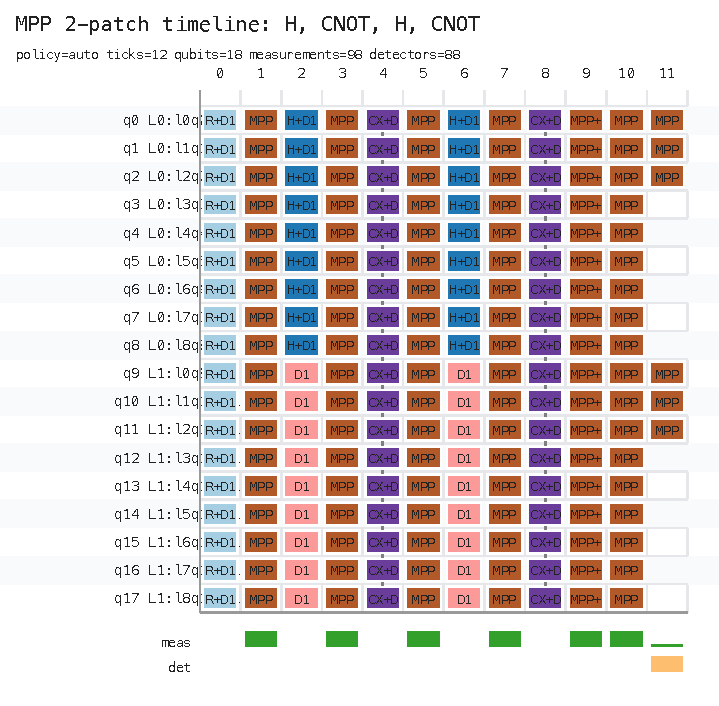
\includegraphics[width=\linewidth]{figures/ch24_stim_timeline.pdf}
  \caption{\texttt{stim\_timeline\_visualizer.py} の実出力。論理量子ビット 2 個に $H$、$\mathrm{CNOT}$、$H$、$\mathrm{CNOT}$ を順に適用した MPP 回路を \texttt{tick\_policy="auto"}・\texttt{stride=9} で可視化しています（tick 数 12、物理量子ビット 18 個、測定 98 回、検出器 88 個）。行ラベルは \texttt{q0 L0:l0} のように論理パッチ \texttt{L} と局所番号 \texttt{l} に分解されています。$H$ は $L0$ の 9 量子ビット全体にかかる transversal H（青）、$\mathrm{CNOT}$ は 2 パッチ間の transversal CX（紫）で、対応する量子ビットが縦線で結ばれます。褐色は MPP によるスタビライザ測定ラウンドです。}
  \label{fig:ch24_stim_timeline}
\end{figure}

\texttt{stride} を渡すと、行ラベルが \texttt{q7 L0:l7} のように「論理 \texttt{L}・局所 \texttt{l}」へ分解され、論理パッチごとのまとまりが読めます。
このとき manifest には、tick ごとに活動している論理パッチ数の分布（\texttt{patch\_concurrency\_counts}）も入ります。

\begin{warningbox}
  \texttt{explicit} ポリシーを \texttt{TICK} の無い回路に適用すると、全命令が 1 つの巨大な tick に潰れてしまいます。
  このモジュールはその状況を検出し、HTML に「\texttt{--tick-policy auto} を使うと量子ビット衝突を避けて自動でタイムスライス化できる」旨の警告を出します。
  MPP レベルのトイ回路では \texttt{auto} を既定にするのが安全です。
\end{warningbox}

\section{T 分岐可視化}\label{sec:t_branch}

\texttt{t\_branch\_visualizer.py} は、非クリフォードの $T$／$T^\dagger$ をゲートカット（QPD）で符号付きクリフォード分岐に展開する様子を描きます。
$T$ の分解は次の 3 項です。

\[
T = \tfrac12 I + \tfrac{1}{\sqrt2}\,S - \tfrac{\sqrt2-1}{2}\,Z,
\qquad
T^\dagger = \tfrac12 I + \tfrac{1}{\sqrt2}\,S^\dagger - \tfrac{\sqrt2-1}{2}\,Z.
\]

\begin{lstlisting}[language=Python, caption={T の QPD 項（src/ftqc/viz/t\_branch\_visualizer.py）}]
SQRT2 = math.sqrt(2.0)
T_QPD_TERMS = (
    ("I", 0.5),
    ("S", 1.0 / SQRT2),
    ("Z", -(SQRT2 - 1.0) / 2.0),
)
\end{lstlisting}

係数の絶対値の和がその $T$ の $\gamma$ で、$\gamma = \tfrac12 + \tfrac{1}{\sqrt2} + \tfrac{\sqrt2-1}{2} = \sqrt2$ です。
$T$ が $k$ 個あれば分岐は $3^k$ 本、全体の $\gamma$ は $(\sqrt2)^k$、モンテカルロ推定の分散オーバーヘッドは $\gamma^2$ になります。
図の読み方の要点は、分岐の\textbf{行き先}です。

\begin{itemize}
  \item \textbf{$I$／$Z$ 分岐}はクリフォードのみなので、通常の Stim／クリフォード QEC チャンクへ流せます。
  \item \textbf{$S$／$S^\dagger$ 分岐}は位相ゲートなので、\texttt{LS-S} シェル（第 IV 部）へルーティングされます。図では黄色でマークされ、各分岐に \texttt{...\_ls\_s\_shell} というシェルラベルが付きます。
\end{itemize}

分岐ツリーの SVG は、$T$ の数だけ深さが増え、各ノードにその接頭辞までの累積係数が表示されます。
負係数（$Z$ 項）を通った分岐は赤系の色で描かれ、これが後処理の符号付き推定量で負の重みを持つことを示します。
分岐数が既定の上限（\texttt{max\_branches=243}、すなわち $3^5$）を超えると、ツリーは省略され「JSON／表を見よ」という案内に切り替わります。これが「巨大ログを載せすぎない」ための実装上の歯止めです。

このモジュールは小さな NumPy 状態ベクトルで理想分布も計算し、QPD 再構成分布・有限ショットの符号付き推定量・理想 $T$ 分布を並べて表示します。
符号付き推定量に小さな負値が出ることがあるのは仕様であり（$Z$ 分岐の負係数を後処理で復元するため）、バグではない——この判断を図が支えます。

\section{実行レポート}\label{sec:reports}

前 3 節のツールは層ごとの単体ビューでした。
残る 3 モジュールは、それらを\textbf{同一の run／操作}について 1 ページに合成します。

\subsection{ftqc\_integrated\_report.py}

\texttt{ftqc\_integrated\_report.py} は、1 つの格子手術操作を 3 つの視点で縦に積みます。
(1) アーキテクチャ／依存グラフ、(2) 論理 $\to$ 物理マッピング、(3) 実行時系列（tick）です。
依存グラフは第18章の 7 ファイル図（\texttt{fig:deps}）に対応し、選んだ操作が使うファイルを橙色で強調します。

\begin{lstlisting}[language=Python, caption={操作ごとの強調ファイル（src/ftqc/viz/ftqc\_integrated\_report.py）}]
_OP_HIGHLIGHT = {
    "merge_zz": {"sh", "cm", "gm"},
    "cnot":     {"sh", "cn", "gm"},
    "t":        {"sh", "cn", "tg", "gm"},
    ...
}
\end{lstlisting}

3 つの視点は同じビルダ実体から生成されるので、「同じ回路を 3 つの角度から見ている」ことが保証されます。

\subsection{ftqc\_run\_visualizer.py}

\texttt{ftqc\_run\_visualizer.py} は、現行 runtime の \texttt{plan(gates)} を可視化へ配線する\textbf{非侵襲}なブリッジです。
\texttt{HybridFTQCRuntime} は各イベントの Stim 回路を内部で構築して即サンプル・デコードし、回路自体を \texttt{QECReport} に保持しません。
そこでこのブリッジは、plan の各イベントに対して可視化用の代表回路を構築し、タイムラインへ渡します。LS-CNOT イベントには LS-CNOT ビルダを使います。空の Clifford chunk と単独の S/T イベントは汎用の memory 回路で表します。これらは statevector 経路の内部回路や、QPD の全分岐を記録した実行トレースではありません。

\begin{lstlisting}[language=Python, caption={plan のイベントを回路へ再構築（src/ftqc/viz/ftqc\_run\_visualizer.py, 要約）}]
for ev in runtime.plan(gates):
    if isinstance(ev, CliffordChunk):
        circ = _clifford_circuit(ev.gates, n, p, tail)
    elif isinstance(ev, LSCnotEvent):
        circ = build_ls_cnot_shell(p=p, noise=True).circuit
        ls_builder = LSCnotFT()          # マッピング図用のビルダ実体
    elif isinstance(ev, SpecialGate):
        circ = _clifford_circuit([], n, p, tail)  # 汎用 memory 回路による代表表示
\end{lstlisting}

こうして「論理ゲート列 $\to$ イベントごとの代表回路 $\to$ tick」を一望できます。これは runtime が実際に実行した全回路の記録ではありません。
$T$ を含む場合は、同じゲート列を \texttt{t\_branch\_visualizer} にも渡して QPD の分岐構造を別に表示します。QPD モードでは $I/Z$ 分岐が memory 経路、$S/S^\dagger$ 分岐が LS-S に対応しますが、run レポートは全分岐の実行トレースではありません。

\subsection{ftqc\_run\_report.py}

\texttt{ftqc\_run\_report.py} は、1 つの run を \textbf{4 視点}で 1 ページに束ねるレポートです。T 用 QEC モデルとして実装されているのは memory のみです。
(1) 依存グラフ（全イベントが使うファイルの和集合を強調）、(2) ベースの論理 $\to$ 物理（\texttt{mpp\_d3} データパッチ）、(3) イベント別の（LS ならマッピング $+$）tick、(4) $T$ を含むなら QPD 分岐です。
3 つの可視化と 2 つのブリッジをライブラリとして合成します。依存図、イベント一覧、QPD 図は同じ入力ゲート列と plan を基にしますが、タイムラインは上記の代表回路を示します。

\begin{lstlisting}[language=Python, caption={4 視点レポートの合成（src/ftqc/viz/ftqc\_run\_report.py, 要約）}]
rt = HybridFTQCRuntime(n_logical, p_phys=p_phys, cnot_mode=cnot_mode,
                       nonclifford_mode=nonclifford_mode)
evs = event_circuits(rt, gates)                 # 同じ plan を共有
highlight = set().union(*[e["highlight"] for e in evs])
dep_svg   = build_dependency_svg(highlight)     # (1) 依存グラフ
base_map  = fmv.build_mpp_assignment(n_logical, ...)   # (2) ベース割り当て
# (3) 各イベントの代表回路のタイムライン、(4) T の QPD 分岐図
\end{lstlisting}

読むときは上から下へ、抽象（どのファイル・どの論理割り当て）から具体（tick ごとの物理操作・分岐）へ降りていくのが定石です。

\section{やること・スコープ外}\label{ch24:scope}

\subsection{やること}

\begin{itemize}
  \item 3 つの割り当てモデル（\texttt{mpp\_d3}／\texttt{generated\_d3}／\texttt{ls}）のマッピング図の読み方と、seam アンシラの意味を示す。
  \item Stim タイムラインの 3 つの tick ポリシーと、tick $\times$ 物理量子ビットの図・2 量子ビット接続・測定/検出器バーの読み方を示す。
  \item $T$ の QPD 分岐（$\gamma=\sqrt2$、$3^T$ 分岐、$S$ 分岐の LS-S ルーティング、符号付き推定量）の図の読み方を示す。
  \item 3 つのレポート（integrated／run\_visualizer／run\_report）が同一 run を複数視点で合成する仕組みを示す。
\end{itemize}

\subsection{スコープ外}

\begin{itemize}
  \item 可視化が読み取る対象そのものの正しさ（デコード・残差注入・符号距離）は前章までとテスト章（第25章）の主題であり、本章は「既に計算された構造を図にする」層に限定します。
  \item HTML／SVG のスタイル詳細やブラウザ互換性など、表示技術の作り込みには踏み込みません。
  \item 本書ではシンプレクティックフレームや qLDPC 配置の可視化は扱いません。
\end{itemize}

\section{まとめ}\label{ch24:summary}

\begin{itemize}
  \item \texttt{ftqc\_mapping\_visualizer.py} は論理 $\to$ 物理を 3 モデルで描き、格子手術では seam（複数パッチにまたがる）アンシラを赤で強調します。
  \item \texttt{stim\_timeline\_visualizer.py} は Stim テキストを tick に分割し、物理量子ビット $\times$ tick の活動・2 量子ビット接続・測定/検出器バーを描きます。\texttt{TICK} の無い回路では \texttt{auto} ポリシーが安全です。
  \item \texttt{t\_branch\_visualizer.py} は $T$ を $\tfrac12 I + \tfrac{1}{\sqrt2}S - \tfrac{\sqrt2-1}{2}Z$ に展開し、$S$ 分岐を LS-S シェルへ、$I/Z$ 分岐をクリフォード QEC へ振り分けた分岐ツリーを描きます。分岐数が多すぎると図を省略します。
  \item \texttt{ftqc\_integrated\_report.py}／\texttt{ftqc\_run\_visualizer.py}／\texttt{ftqc\_run\_report.py} は、これらを同一 run／操作について 3〜4 視点に合成します。特に run\_visualizer は runtime を改変しない非侵襲ブリッジです。
\end{itemize}

\subsection*{合否基準での検証}

本章の可視化は正解を生む層ではないので、合否基準そのものを判定するのはテスト章（第25章）に譲ります。
ただし可視化は、合否基準の\emph{目視確認}を支えます。
たとえばマッピング図で seam アンシラが期待した縫い目にだけ現れること、タイムラインの検出器バーがノイズなしで gauge を誤検出していないこと、$T$ 分岐図の理想分布と QPD 再構成が一致していること——これらは、\texttt{shortest\_graphlike\_error}$=d$ や「\texttt{decode\_shell} が \texttt{allow\_gauge\_detectors} を使わない」といった機械的基準を、人間の側から裏取りする材料になります。
また 3 つのレポートは同一の runtime／plan から生成されるため、4 視点が食い違って見えたら、それ自体が「どこかの層で設定がずれている」というシグナルになります。

次章では、こうした目視確認を機械的な不変条件テスト・統計テスト・性能評価へと昇格させ、Stage 03（$d=3$ 統合）の到達点を宣言します。

\begin{exercise}
  \begin{enumerate}
    \item \texttt{mpp\_d3} モデルで \texttt{stride=9} のとき、論理量子ビット $2$ の $X_L$ 台 \texttt{XL=[0,3,6]} に対応する物理添字を求めなさい。\texttt{build\_mpp\_assignment} の \texttt{physical = q*stride + local} を用いて説明しなさい。
    \item \texttt{stim\_timeline\_visualizer.py} で、\texttt{TICK} を含まない回路に \texttt{explicit} ポリシーを適用すると何が起きるか、また HTML にどんな警告が出るかを述べ、代わりにどのポリシーを使うべきか答えなさい。
    \item $T$ ゲートを 3 個含む回路では、QPD 分岐は何本になり、全体の $\gamma$ と分散オーバーヘッド $\gamma^2$ はいくつになるかを求めなさい。
    \item \texttt{ftqc\_run\_visualizer.py} が runtime のイベント回路を「非侵襲に」再構築すると言えるのはなぜか、\texttt{HybridFTQCRuntime} が回路を \texttt{QECReport} に保持しないという事実と、同じ公開ビルダを呼び直すという方針から説明しなさい。
  \end{enumerate}
\end{exercise}

% Stage: 03 ／ 説明用コード: src/ftqc（合否基準の言語は src/ftqc 整合）
\chapter{テストと性能評価}\label{ch:testing_perf}

\begin{chaptergoal}
  \begin{itemize}
  \item ノイズなしでの gauge 検出器ゼロ・回路レベル距離・真理値表・$35p^3$ という、Stage 03 が満たすべき不変条件テストを理解します。
  \item 固定シードと閾値で統計テストを安定化し、回帰（リグレッション）として運用する考え方を理解します。
  \item transversal 操作と格子手術のコストの違いと、距離 $d=3$ での論理エラー率の $\sim p^2$ スケーリングの直感を理解します。
  \item デコード遅延・ストールという性能ボトルネックの簡易モデルを理解します。
  \item Stage 03 の到達点（$d=3$ 統合の完成）と、残差が $X_L$ 中心であるという限界を確認し、読了マーカー C を宣言します。
  \end{itemize}
\end{chaptergoal}

前章までで、$d=3$ に固定した統合シミュレータ \texttt{HybridFTQCRuntime} の全体像——命令計画、トラジェクトリ実行と残差注入、状態ベクトルバックエンド、可視化とレポート——が出そろいました。
本章では、この Stage 03 の成果物が「正しく動いている」ことをどう機械的に確かめるかを整理します。
検証は大きく 2 系統に分かれます。ひとつは入力に対して決定論的に成り立つべき\textbf{不変条件テスト}、もうひとつはモンテカルロ由来のばらつきを固定シードと閾値で押さえた\textbf{統計テスト}です。
最後に性能と誤差収支の見取り図を与え、Stage 03 の限界（残差が $X_L$ 中心であること）を明示します。

\begin{notebox}
  Stage: \textbf{03}。
  説明用コードは主に \codepath{src/ftqc/} の各モジュールの \texttt{demo()} / \texttt{main()} を用います。
  検査コードはリポジトリ直下の \codepath{tests/} にあります。
\end{notebox}

\section{不変条件テスト}\label{sec:invariants}

不変条件テストは、乱数に依存せず、ノイズなしの理想入力に対して必ず成り立つべき性質を検査します。
Stage 03 の中心的な不変条件は次の 4 つです。

\subsection{gauge 検出器ゼロ}

最も重要なのは、\textbf{ノイズなしなら検出器がひとつも発火しない}ことです。
発火する検出器が残っていれば、それはゲージ自由度が測定回路に漏れていることを意味し、その検出器を \texttt{allow\_gauge\_detectors} で無視して回避するとデコードの距離が崩れます。
本書の合否基準では、シェルはすべて gauge 検出器がゼロになるように構成し、\texttt{decode\_shell} は \texttt{allow\_gauge\_detectors} を\textbf{使わない}ことを要求します。
\codepath{src/ftqc/ls_handoff_shells.py} の \texttt{demo()} は、各シェルについてノイズなしの検出器サンプルを取り、発火した検出器の本数を数えて確認します。

\begin{lstlisting}[language=Python, caption={gauge 検出器ゼロの確認（src/ftqc/ls\_handoff\_shells.py の demo() から要約）}]
clean = builder(p=0.0, noise=False)
det, _ = clean.circuit.compile_detector_sampler().sample(2000, separate_observables=True)
nd = int(det.any(axis=0).sum())   # 一度でも発火した検出器の本数
# nd == 0 であること = gauge 検出器ゼロ = allow_gauge_detectors 不要
\end{lstlisting}

\subsection{回路レベル距離の graphlike 上界}

次に、ノイズありの回路から検出器誤りモデル（DEM）を構築し、非 graphlike 誤りを無視した \texttt{shortest\_graphlike\_error()} の長さを測ります。
ここで \texttt{decompose\_errors=True} は、分解可能な複合誤りを graphlike な成分へ分解する要求です。gauge detector を許可するかどうかは独立した \texttt{allow\_gauge\_detectors} 引数で指定し、その既定値は \texttt{False}（非決定論的 detector を拒否）です。以下では二つの意図を別々の引数として明示します。
独立シェル API（LS-S・LS-CNOT・LS-T）は距離 $d=3$ のパッチを意図しており、公開テストは graphlike 上界を検査します。ただし、未分解 DEM に高次誤り機構がある場合、これは FT 性の厳密な証明ではありません。

\begin{lstlisting}[language=Python, caption={回路レベル距離の確認（src/ftqc/ls\_handoff\_shells.py の demo() から要約）}]
noisy = builder(p=0.005, noise=True)
noisy.circuit.detector_error_model(
    decompose_errors=True,        # 分解可能な複合誤りを graphlike 成分へ分解
    allow_gauge_detectors=False,  # 非決定論的 detector を拒否（既定値）
)
bound = len(noisy.circuit.shortest_graphlike_error(ignore_ungraphlike_errors=True))
# bound == 3: パッチ距離 3 と整合する回路距離の上界
\end{lstlisting}

未分解 DEM の全物理誤り機構が graphlike であることまで確認できたシェルに限り、この値を厳密距離と呼べます。単に \texttt{decompose\_errors=True} が成功しただけでは、graphlike 成分数と物理 fault 数が一致する保証はありません。

\subsection{真理値表一致}

論理演算そのものが正しいかは、計算基底の真理値表で確かめます。
たとえば LS-CNOT では、制御と対象を $\ket{0_L}/\ket{1_L}$ の 4 通りに準備し、生サンプルから得た論理値の絶対値（フレーム補正後の観測量）が CNOT の真理値表と全一致することを検査します。

\begin{lstlisting}[language=Python, caption={CNOT 真理値表の確認（src/ftqc/ls\_cnot\_ft.py の demo() の [C] から要約）}]
# 制御・対象を |0_L>,|1_L> の 4 通りに準備し、
# フレーム補正した観測量が CNOT 真理値表と一致するかを検査する。
print(f"    真理値表: {'全一致 OK (CNOT を正しく実装)' if ok_all else 'NG'}")
\end{lstlisting}

この例では gauge 検出器ゼロ・graphlike 距離上界 $3$・真理値表一致が、選んだ入力の論理動作と整合します。これらの確認だけで一般の fault-tolerance 性が証明されるわけではなく、その主張には追加の検証が必要です。

\subsection{$35p^3$：蒸留の 3 次抑圧}

非クリフォード側の不変条件は magic state 蒸留にあります。
$[[15,1,3]]$ Reed--Muller 符号を使った 15-to-1 蒸留では、検出されない論理 $X$ 誤りのうち重み 3 のものがちょうど 35 個あり、出力誤り率が入力誤り率 $p$ の 3 次で $p_{\mathrm{out}} \sim 35\,p^3$ と抑圧されます。
\codepath{src/ftqc/t_gate.py} の符号重み分布から、重み 3 の未検出論理誤りが 35 個あることを数えられます。この組合せ論的な係数は小さい $p$ における先頭項であり、一般の有限 $p$ で出力誤り率が厳密に $35p^3$ になるという主張ではありません。

\begin{lstlisting}[language=Python, caption={蒸留の 3 次抑圧の確認（src/ftqc/t\_gate.py の demo() から要約）}]
# 重み3 の undetected-logical X 誤りがちょうど 35 個 -> 出力誤り ~ 35 p^3
for p in (0.01, 0.02, 0.05):
    acc, pout = distill(HX, HZ, p)
    print(f"{p:.3f} | accept={acc:.3f} | p_out={pout:.2e} | 35 p^3={35*p**3:.2e} | ratio={pout/(35*p**3):.2f}")
# => ratio が 1 付近 = 3 次抑圧を確認
\end{lstlisting}

ランタイム側では、\texttt{magic\_distillation\_shots=0}（既定）のとき、この決定論的な先頭項 $35\,p_{\mathrm{phys}}^3$ をそのまま magic fault 率として使います（\texttt{\_estimate\_magic\_error()} が \texttt{min(1.0, 35.0 * self.p\_phys ** 3)} を返す）。
\texttt{magic\_distillation\_shots} を正の値にすればモンテカルロ推定に切り替わりますが、いずれにせよ「$p^3$ で抑圧される」という不変条件は変わりません。

\section{統計テストの安定化}\label{sec:stats}

不変条件テストと違い、論理分布や残差率はモンテカルロで推定するため、実行のたびに数値がわずかに揺れます。
これをテストとして運用するには、揺れを再現可能にし、合否の閾値を明示する必要があります。

\subsection{固定シード}

\texttt{HybridFTQCRuntime} は \texttt{seed} をコンストラクタ引数に取り、\texttt{run(program, shots, seed=...)} でもシードを渡せます。公開テストでは同じプログラム・同じ seed で出力が一致するかを比較します。ただし、このテストは \texttt{qec\_mode="off"} で実行され、QEC sampling の再現性を対象にしていません。runtime の Stim sampler 呼び出しは seed を受け取らないため、QEC を有効にした実行の再現性は未確認です。

\begin{lstlisting}[language=Python, caption={固定シードでの再現（src/ftqc/hybrid\_ftqc\_runtime.py の demo() から要約）}]
rt = HybridFTQCRuntime(n_logical=1, p_phys=0.0, seed=31, qec_mode="off")
first = rt.run(program, shots=600, seed=91)
second = rt.run(program, shots=600, seed=91)
assert first.measurement_counts == second.measurement_counts
\end{lstlisting}

\subsection{閾値}

固定シードで数値が決まっても、統計テストは「厳密一致」ではなく「許容誤差内」で判定します。
たとえば前章で見たバックエンド間比較では、理想分布どうしの全変動距離（TVD）が十分小さいことを閾値で判定しました。
残差率であれば、ノイズなしなら\textbf{厳密にゼロ}（不変条件）、ノイズありなら\textbf{ゼロでない}（存在するかどうかの真偽）という質的な閾値の立て方が安定です。
残差モードの挙動を追加評価する場合は、同梱コードが実際に提供する API を確認し、ノイズなしでのゼロ残差とノイズありでの残差分布を分けて測定します。

\subsection{リグレッション例}

こうしたテストは、実装をいじったときに壊れていないかを見張る回帰（リグレッション）として働きます。
回帰テストでは、対象 API の既定値や実行経路など、再現可能な構造的性質を検査します。検査を追加した場合は、その実行結果と対象バージョンを合わせて記録してください。

\begin{notebox}
  公開版に含む Stage 03 のテストは import、境界条件、スモーク動作、例の実行可能性を対象にします。ここで述べた追加の数値評価は、実行結果を記録するまでは未確認として扱います。
\end{notebox}

\section{性能と誤差収支}\label{sec:perf}

\subsection{transversal と格子手術のコスト}

論理演算の実現手段には、生成子追跡で済む transversal 操作と、補助パッチ・複数ラウンドの測定を要する独立シェル API（LS-CNOT・LS-S・LS-T）があります。Stage 03 runtime が格子手術イベントとして扱うのは LS-CNOT です。
前者はスタビライザ生成子の書き換えだけで完結し、追加の QEC ラウンドや補助量子ビットをほとんど必要としません。
後者は merge/split のために \texttt{ls\_merge\_rounds} 分の追加ラウンドと seam 上の安定化子を要し、そのぶんショットあたりのコストと、注入される残差の機会が増えます。
Stage 03 の \texttt{HybridFTQCRuntime} は、可能な操作を transversal 側で処理し、CNOT や $T$ のように格子手術が必要な箇所だけシェルを呼び出す構成になっています。

\subsection{論理エラー率のスケーリング}

距離 $d$ の表面符号は、重み $\lceil d/2 \rceil$ 以上の誤りで初めて論理故障に至ります。
$d=3$ なら 2 個の物理誤りがそろって初めて論理が飛ぶため、論理エラー率は先頭項で
\[
  p_L \;\sim\; \binom{N_{\mathrm{opp}}}{2}\, p^2 \;=\; O(p^2)
\]
のように物理誤り率 $p$ の 2 次で立ち上がります（$N_{\mathrm{opp}}$ は誤りの機会数。一般には $p_L \sim p^{\lceil d/2 \rceil}$）。
一方、magic state 経由の $T$ ゲートは前節の蒸留により $O(p^3)$ で抑圧されるため、概念的な誤差収支では「距離 3 の回路レベル fault 組合せの $O(p^2)$」と「蒸留の先頭項 $35p^3$」を別々に扱います。これらは本書のコードで測定した性能ベンチマークではありません。
この $p^2$／$p^3$ の別勘定は、どこがボトルネックかを $p$ の大きさに応じて切り分ける指針になります。

\section{3 大ボトルネックのモデル化}\label{sec:bottlenecks}

性能面では、シミュレータの外側にある実機由来のボトルネックも簡易にモデル化しておくと、結果の読み方が変わります。
とくに重要なのが\textbf{デコード遅延}と、それに起因する\textbf{ストール}です。

論理サイクルごとにシンドロームが生成され、デコーダがそれを処理して補正を返すまでに遅延 $t_{\mathrm{dec}}$ がかかります。
論理サイクル時間を $t_{\mathrm{cycle}}$ とすると、遅延がサイクルに追いつかない場合、すなわち $t_{\mathrm{dec}} > t_{\mathrm{cycle}}$ のとき、後続の論理演算は待たされます。
この待ち（ストール）を最小限にモデル化すると、実効的な論理サイクル時間はおよそ
\[
  t_{\mathrm{eff}} \;\approx\; \max(t_{\mathrm{cycle}},\, t_{\mathrm{dec}})
\]
となり、$T$ ゲートのように結果に依存した補正（測定してから $S$ 補正を決める）を挟む箇所では、デコード結果を待つぶんの直列化がさらに乗ります。
Stage 03 のシミュレータ自体はこの実時間を扱いませんが、「格子手術のラウンド数」「$T$ テレポートの測定→補正の直列依存」という構造は、そのままデコード遅延・ストールが効く箇所を指し示しています。

\begin{notebox}
  ここでの遅延・ストールのモデルは\textbf{簡易な見取り図}であり、Stage 03 の数値には反映されません。窓デコード（windowed decoding）による遅延の隠蔽など、より本格的なスケジューリングは本書の対象外です。
\end{notebox}

\section{Stage 03 の到達点}\label{sec:stage_c_marker}

\subsection{$d=3$ 統合の完成}

ここまでで、Stage 03 の目標であった「$d=3$ に固定した、QEC とトラジェクトリと状態ベクトルを貫くハイブリッドシミュレータ」が完成しました。
具体的には、\texttt{HybridFTQCRuntime} が

\begin{itemize}
  \item クリフォード操作を生成子追跡または runtime の LS-CNOT 経路へ振り分け、S/T の汎用 handoff と独立した LS-S／LS-T シェル API を区別し、
  \item 各シェルが gauge 検出器ゼロ・\texttt{shortest\_graphlike\_error}$=3$・真理値表一致を満たし、
  \item 非 Clifford $T$ を状態ベクトルまたは QPD で扱い、magic fault 率のモデルに $35p^3$ の先頭項を使い、
  \item QEC シェルから得た残差をパウリフレームとして論理状態へ注入する、
\end{itemize}

という一連の流れを同一シードで再現できるかを、公開テストで検査します。

\subsection{残差が $X_L$ 中心であるという限界}

一方で、Stage 03 の残差経路には本質的な限界があります。
現状の Stim コンパイラが物理的に露出させているのは $Z$ 観測量のフリップ、すなわち残差 $X_L$ フォールトが中心です。
$Z_L$ 側の残差は、\texttt{mirror\_z\_residuals} のように「$X_L$ と同じ率で独立に $Z_L$ を振る」近似で補うか、公開 API では独立な近似チャネル \texttt{mirror\_z\_residuals} を選ぶことができます。
つまり Stage 03 のフレームは、$X_L$ と $Z_L$ を対等・相関ありに扱う完全なパウリフレームには\textbf{まだなっていません}。
シンプレクティックなパウリフレームへの一般化は本書の対象外です。

\subsection{読了マーカー C}

\begin{notebox}
  \textbf{読了マーカー C を宣言します。}
  ここまでで Stage 01（現象論 MPP）・Stage 02（回路レベル）・Stage 03（$d=3$ 統合）を通読し、$d=3$ に固定した誤り耐性ハイブリッドシミュレータを、合否基準つきで動かせる状態に到達しました。
  本書ではこのモデル範囲を明記し、結果の解釈に含めます。
\end{notebox}

\section{合否基準チートシート（再掲）}\label{sec:cheatsheet_c}

Stage 03 のモデル範囲で確認すべき性質を整理します。

\begin{itemize}
  \item \textbf{gauge 検出器ゼロ}：ノイズなしで発火する検出器が 1 本もない。したがって \texttt{decode\_shell} は \texttt{allow\_gauge\_detectors} を\textbf{使わない}。
  \item \textbf{graphlike 上界}：公開テスト対象のシェルで \texttt{shortest\_graphlike\_error()} の値を検査します。これだけで厳密距離が証明されるわけではありません。
  \item \textbf{真理値表一致}：計算基底で論理演算の真理値表が全一致する（フレーム補正後）。
  \item \textbf{$35p^3$ の先頭項}：15-to-1 蒸留符号で重み 3 の未検出論理誤りが 35 個あります。これは低確率での先頭項です。
  \item \textbf{シード再現性}：QEC を含む経路で Stim sampler に seed が渡ることを含めて確認する（現行公開 runtime では未達）。
  \item \textbf{残差モデルの制限}：ノイズなしのシェルで残差が生じないことを確認し、$X_L$ 中心というモデル範囲を結果に添える。
\end{itemize}

\section{やること・スコープ外}\label{ch25:scope}

\subsection{やること}

\begin{itemize}
  \item Stage 03 で検査すべき不変条件と、実行前に結果を断定しない報告方法を説明する。
  \item モンテカルロ由来のばらつきを固定シードと閾値で押さえ、回帰として運用する考え方を示す。
  \item transversal と格子手術のコスト差、$p_L \sim p^2$ のスケーリング、デコード遅延・ストールの簡易モデルを示す。
  \item Stage 03 の到達点と、残差が $X_L$ 中心である限界を明示する。
\end{itemize}

\subsection{スコープ外}

\begin{itemize}
  \item シンプレクティックフレーム、qLDPC、窓デコード、消失ノイズのテスト詳細。これらは本書の対象外です。
  \item デコード遅延・ストールの本格的なスケジューリングと窓デコードによる隠蔽（本書の対象外）。
  \item 実時間・実機データを用いた性能ベンチマーク。本章の性能評価はあくまで構造的な見取り図にとどめます。
\end{itemize}

\section{まとめ}\label{ch25:summary}

\begin{itemize}
  \item 不変条件テストは、ノイズなし検出器、graphlike 上界、CNOT 真理値表、および蒸留符号の組合せ論的性質を検査します。
  \item 再現性テストは QEC を無効にした runtime 経路で固定 seed の出力を比較します。QEC sampling の再現性は今後の検証課題です。
  \item 最小重みの議論から、距離 3 では低確率領域の論理誤りが概ね $O(p^2)$、15-to-1 蒸留の先頭項は $35p^3$ と見積もれます。デコード遅延・ストールは $t_{\mathrm{eff}} \approx \max(t_{\mathrm{cycle}}, t_{\mathrm{dec}})$ という簡易モデルで見取り図が描けます。
  \item Stage 03 は $d=3$ 統合の完成をもって読了マーカー C に到達しますが、残差が $X_L$ 中心であるという限界を残しており、この制限を付録Cで明示します。
\end{itemize}

\subsection*{合否基準での検証}

公開テストが対象にする性質は次のとおりです。これらをここで再実行したという意味ではありません。

\begin{itemize}
  \item \texttt{tests/test\_ls\_invariants.py} は LS-S／LS-CNOT／LS-T のノイズなし検出器と graphlike 上界を検査し、LS-CNOT の計算基底真理値表も確認します。
  \item \texttt{tests/test\_magic\_state.py} は蒸留符号の距離と重み 3 の未検出論理誤り数（35）を検査します。有限確率でのモンテカルロ比の評価は含みません。
  \item \texttt{tests/test\_runtime\_reproducibility.py} は同じ seed での runtime 出力再現性を検査します。
\end{itemize}

$X_L$ と $Z_L$ を相関付きで対等に扱う論理パウリフレームは、本書では実装していません。

本章で示した $d=3$ 固定の統合ランタイムが、本書の到達点です。

\begin{exercise}
  \begin{enumerate}
    \item ノイズなしで発火する検出器が 1 本でも残っている場合、なぜそれを \texttt{allow\_gauge\_detectors} で無視するとデコード距離が崩れるのかを、本章の不変条件テストの意図に沿って説明しなさい。
    \item $d=3$ の表面符号で論理エラー率が $\sim p^2$ になる理由を、論理故障に必要な最小誤り重みの観点から述べなさい。$d=5$ ではどうなるか、$p^{\lceil d/2\rceil}$ の式に当てはめて答えなさい。
    \item 15-to-1 蒸留の出力誤りが $35p^3$ になるときの「35」が何を数えた数かを、\texttt{t\_gate.py} の \texttt{demo()} が印字する重み分布に基づいて説明しなさい。
    \item デコード遅延 $t_{\mathrm{dec}}$ が論理サイクル時間 $t_{\mathrm{cycle}}$ を超える場合、$T$ ゲートのテレポート（測定→$S$ 補正の直列依存）がなぜとくにストールを受けやすいかを、本章のボトルネックモデルに沿って述べなさい。
    \item Stage 03 の残差が $X_L$ 中心であることを、\texttt{mirror\_z\_residuals} が「近似」であるという本文の記述と結びつけて説明し、これを完全なパウリフレームにするには何が足りないかを述べなさい。
  \end{enumerate}
\end{exercise}

% ----- 結び -----
\chapter*{結び}
\addcontentsline{toc}{chapter}{結び}
本書では、単一の安定化器シミュレーションから始め、格子手術の論理操作と回路レベルの検査を経て、固定距離のハイブリッドランタイムまでを実装しました。各段階の結果はモデルの前提に依存します。特に $d=3$ の評価や簡略化した残差注入だけから、大規模な FTQC の性能や一般の論理故障率を結論することはできません。次の実装へ進む際も、検査が示す上界・統計的推定・決定論的性質を分けて報告することが大切です。

\appendix
\part{付録}\label{part:appendix}

% 付録A — 開発環境セットアップ
\chapter{開発環境セットアップ}\label{app:setup}

本書のコードは Python 3.12 以降と uv を使います。Stage 01、Stage 02、Stage 03 は同じ \texttt{ftqc} という import 名を持ちますが、依存関係と実装が異なる独立したプロジェクトです。混在を避けるため、それぞれのディレクトリで環境を同期して実行してください。

\section{Stage 01}

リポジトリのルートから次を実行します。
\begin{lstlisting}[language=bash]
uv sync --directory src/stages/01_mpp --locked
uv run --directory src/stages/01_mpp --locked pytest -q
uv run --directory src/stages/01_mpp --locked python examples/ch06_surface_patch.py
\end{lstlisting}

\section{Stage 02}

\begin{lstlisting}[language=bash]
uv sync --directory src/stages/02_circuit_level --locked
uv run --directory src/stages/02_circuit_level --locked pytest -q
uv run --directory src/stages/02_circuit_level --locked python examples/ch16_circuit_merge.py
\end{lstlisting}

\section{Stage 03}

Stage 03 はリポジトリ直下の \texttt{pyproject.toml} と \texttt{uv.lock} を使います。
\begin{lstlisting}[language=bash]
uv sync --locked
uv run --locked pytest -q tests
uv run --locked python examples/ch25_d3_benchmark.py
\end{lstlisting}

書籍 PDF を生成する場合は LuaLaTeX と latexmk が必要です。\texttt{book/} で \texttt{latexmk -lualatex main.tex} を実行します。依存パッケージの導入方法は利用する OS の公式手順に従ってください。

% 付録B — モジュール地図
\chapter{モジュール地図}\label{app:modules}

各 Stage のモジュール対応を機械可読な一覧として \texttt{book/code-map.toml} に収録しています。本付録では実行環境と役割の関係を示します。

\begin{description}
  \item[Stage 01: \texttt{src/stages/01\_mpp/}] MPP による現象論モデルです。\texttt{surface\_patch.py} と \texttt{clifford\_ft\_full.py} がパッチ・論理 Clifford を扱い、\texttt{geom\_lattice\_surgery.py}、\texttt{lattice\_surgery.py}、\texttt{ls\_handoff\_shells.py} が論理格子手術を構成します。\texttt{t\_gate.py} と \texttt{qpd\_backend.py} は蒸留模型と QPD を担います。
  \item[Stage 02: \texttt{src/stages/02\_circuit\_level/}] ancilla によるシンドローム抽出と回路レベル誤りを扱います。\texttt{circuit\_level\_merge.py} が merge 回路、\texttt{ls\_cnot\_ft.py} が論理 CNOT と T teleportation shell、\texttt{ls\_handoff\_shells.py} が検出器付き handoff 回路を構築します。
  \item[Stage 03: \texttt{src/ftqc/}] Stage 01・02 の要素を距離 $d=3$ のランタイムに統合します。ルートの \texttt{tests/} と \texttt{examples/} がこの環境に対応します。
\end{description}

Stage 01 と Stage 02 の各プロジェクトは独立した \texttt{src/ftqc}、\texttt{tests/}、\texttt{examples/}、\texttt{pyproject.toml} を持ちます。Stage 03 の正本はルートです。古いディレクトリ名や開発時の設計資料を参照せず、本書に同梱した対応表とソースを使ってください。

% 付録C — 検証と制限
\chapter{検証の読み方とモデルの制限}\label{app:validation}

テストやデモが示す性質の種類を区別してください。決定論的な検査は特定入力に対する恒等式や真理値表を確かめます。統計検査は有限ショットの推定値であり、乱数シード、ショット数、判定閾値とともに解釈します。距離計算が \texttt{shortest\_graphlike\_error()} を使う場合、その値は graphlike 誤りモデルの範囲での上界です。未分解の全誤り機構について別途条件を確認できない限り、符号の厳密距離や一般の FT 性の証明とは呼べません。

公開版には各 Stage のテスト一式と実行例を含めています。テストの存在だけで全項目の実行成功を意味するわけではありません。再現する場合は付録Aのコマンドを実行し、実際の終了コードと出力を記録してください。本文中で個別に示す数値例も、特定の設定・実装に対する結果として扱ってください。

Stage 01 は安定化子を MPP で直接測る現象論モデルであり、局所 ancilla 回路や hook 誤りを表しません。Stage 02 は回路レベルの誤りを導入しますが、任意距離の一般化や実機の全ノイズ過程を含みません。Stage 03 は $d=3$ と 9 個のデータ量子ビットに固定された統合シミュレータです。残差モデルは Stim から得る観測量フリップを中心に構成され、$X_L$ と $Z_L$ の相関を一般に完全に表すものではありません。

したがって、この教材の実行結果から大規模 FTQC の閾値、実機性能、一般の論理誤り率を直接推定することはできません。数値を比較する場合は、回路、ノイズ仮定、デコーダ、距離、サンプリング条件を併記してください。

% 付録D — 参考文献
\chapter{参考文献}\label{app:references}

本文で引用した理論論文、公式ドキュメント、標準教科書およびソフトウェアライブラリを示します。

\begin{thebibliography}{99}

\bibitem{suzuki2026ftqc}
鈴木泰成, 「第2編 第3章 誤り耐性量子計算アーキテクチャ」, 荒川泰彦監修, 『量子イノベーションハンドブック』, エヌ・ティー・エス, 2026年. ISBN: 978-4-86043-492-2 C3050, \url{https://www.nts-book.net/view/item/000000001709}.

\bibitem{gidney2021stim}
Craig Gidney, ``Stim: a fast stabilizer circuit simulator,'' \emph{Quantum}, vol.~5, p.~497, 2021. DOI: \href{https://doi.org/10.22331/q-2021-07-06-497}{10.22331/q-2021-07-06-497}, arXiv: \href{https://arxiv.org/abs/2103.02202}{2103.02202}.

\bibitem{stim2026doc}
Craig Gidney and the Stim contributors, ``Stim v1.16.0: Detector Error Model File Format,'' software documentation, 2026. \url{https://github.com/quantumlib/Stim/blob/v1.16.0/doc/file_format_dem_detector_error_model.md}.

\bibitem{stim2026python}
Craig Gidney and the Stim contributors, ``Stim v1.16.0: Python API Reference (\texttt{stim.FlipSimulator}),'' software documentation, 2026. \url{https://github.com/quantumlib/Stim/blob/v1.16.0/doc/python_api_reference_vDev.md}.

\bibitem{aaronson2004stabilizer}
Scott Aaronson and Daniel Gottesman, ``Improved simulation of stabilizer circuits,'' \emph{Physical Review A}, vol.~70, no.~5, p.~052328, 2004. DOI: \href{https://doi.org/10.1103/PhysRevA.70.052328}{10.1103/PhysRevA.70.052328}, arXiv: \href{https://arxiv.org/abs/quant-ph/0406196}{quant-ph/0406196}.

\bibitem{gottesman1997stabilizer}
Daniel Gottesman, ``Stabilizer Codes and Quantum Error Correction,'' Ph.D. thesis, California Institute of Technology, 1997. arXiv: \href{https://arxiv.org/abs/quant-ph/9705052}{quant-ph/9705052}.

\bibitem{eastin2009transversal}
Bryan Eastin and Emanuel Knill, ``Restrictions on transversal encoded quantum gate sets,'' \emph{Physical Review Letters}, vol.~102, no.~11, p.~110502, 2009. DOI: \href{https://doi.org/10.1103/PhysRevLett.102.110502}{10.1103/PhysRevLett.102.110502}, arXiv: \href{https://arxiv.org/abs/0811.4262}{0811.4262}.

\bibitem{li2015magic}
Ying Li, ``A magic state's fidelity can be superior to the operations that created it,'' \emph{New Journal of Physics}, vol.~17, p.~023037, 2015. DOI: \href{https://doi.org/10.1088/1367-2630/17/2/023037}{10.1088/1367-2630/17/2/023037}, arXiv: \href{https://arxiv.org/abs/1410.7808}{1410.7808}.

\bibitem{fowler2012surface}
Austin G. Fowler, Matteo Mariantoni, John M. Martinis, and Andrew N. Cleland, ``Surface codes: Towards practical large-scale quantum computation,'' \emph{Physical Review A}, vol.~86, no.~3, p.~032324, 2012. DOI: \href{https://doi.org/10.1103/PhysRevA.86.032324}{10.1103/PhysRevA.86.032324}, arXiv: \href{https://arxiv.org/abs/1208.0928}{1208.0928}.

\bibitem{dennis2002topological}
Eric Dennis, Alexei Kitaev, Andrew Landahl, and John Preskill, ``Topological quantum memory,'' \emph{Journal of Mathematical Physics}, vol.~43, no.~9, pp.~4452--4505, 2002. DOI: \href{https://doi.org/10.1063/1.1499754}{10.1063/1.1499754}, arXiv: \href{https://arxiv.org/abs/quant-ph/0110143}{quant-ph/0110143}.

\bibitem{krantz2019guide}
Philip Krantz, Morten Kjaergaard, Fei Yan, Terry P. Orlando, Simon Gustavsson, and William D. Oliver, ``A quantum engineer's guide to superconducting qubits,'' \emph{Applied Physics Reviews}, vol.~6, no.~2, p.~021318, 2019. DOI: \href{https://doi.org/10.1063/1.5089550}{10.1063/1.5089550}, arXiv: \href{https://arxiv.org/abs/1904.06560}{1904.06560}.

\bibitem{chamberland2018frame}
Christopher Chamberland, Pavithran Iyer, and David Poulin, ``Fault-Tolerant Quantum Computing in the Pauli or Clifford Frame with Slow Error Diagnostics,'' \emph{Quantum}, vol.~2, p.~43, 2018. DOI: \href{https://doi.org/10.22331/q-2018-01-04-43}{10.22331/q-2018-01-04-43}, arXiv: \href{https://arxiv.org/abs/1704.06662}{1704.06662}.

\bibitem{horsman2012lattice}
Clare Horsman, Austin G. Fowler, Simon Devitt, and Rodney Van Meter, ``Surface code quantum computing by lattice surgery,'' \emph{New Journal of Physics}, vol.~14, no.~12, p.~123011, 2012. DOI: \href{https://doi.org/10.1088/1367-2630/14/12/123011}{10.1088/1367-2630/14/12/123011}, arXiv: \href{https://arxiv.org/abs/1111.4022}{1111.4022}.

\bibitem{bravyi2005magic}
Sergey Bravyi and Alexei Kitaev, ``Universal quantum computation with ideal Clifford gates and noisy ancillas,'' \emph{Physical Review A}, vol.~71, no.~2, p.~022316, 2005. DOI: \href{https://doi.org/10.1103/PhysRevA.71.022316}{10.1103/PhysRevA.71.022316}, arXiv: \href{https://arxiv.org/abs/quant-ph/0403025}{quant-ph/0403025}.

\bibitem{gidney2019factory}
Craig Gidney and Austin G. Fowler, ``Efficient magic state factories with a catalyzed $\lvert CCZ\rangle$ to $2\lvert T\rangle$ transformation,'' \emph{Quantum}, vol.~3, p.~135, 2019. DOI: \href{https://doi.org/10.22331/q-2019-04-30-135}{10.22331/q-2019-04-30-135}, arXiv: \href{https://arxiv.org/abs/1812.01238}{1812.01238}.

\bibitem{higgott2022pymatching}
Oscar Higgott, ``PyMatching: A Python package for decoding quantum codes with minimum-weight perfect matching,'' \emph{ACM Transactions on Quantum Computing}, vol.~3, no.~3, article~16, 2022. DOI: \href{https://doi.org/10.1145/3505637}{10.1145/3505637}, arXiv: \href{https://arxiv.org/abs/2105.13082}{2105.13082}.

\bibitem{higgott2025sparse}
Oscar Higgott and Craig Gidney, ``Sparse Blossom: correcting a million errors per core second with minimum-weight matching,'' \emph{Quantum}, vol.~9, p.~1600, 2025. DOI: \href{https://doi.org/10.22331/q-2025-01-20-1600}{10.22331/q-2025-01-20-1600}, arXiv: \href{https://arxiv.org/abs/2303.15933}{2303.15933}.

\bibitem{roffe2020bposd}
Joschka Roffe, David R. White, Simon Burton, and Earl T. Campbell, ``Decoding across the quantum low-density parity-check code landscape,'' \emph{Physical Review Research}, vol.~2, no.~4, p.~043423, 2020. DOI: \href{https://doi.org/10.1103/PhysRevResearch.2.043423}{10.1103/PhysRevResearch.2.043423}, arXiv: \href{https://arxiv.org/abs/2005.07016}{2005.07016}.

\bibitem{calderbank1996css}
A. R. Calderbank and Peter W. Shor, ``Good quantum error-correcting codes exist,'' \emph{Physical Review A}, vol.~54, no.~2, pp.~1098--1105, 1996. DOI: \href{https://doi.org/10.1103/PhysRevA.54.1098}{10.1103/PhysRevA.54.1098}, arXiv: \href{https://arxiv.org/abs/quant-ph/9512032}{quant-ph/9512032}.

\bibitem{steane1996qec}
Andrew M. Steane, ``Multiple-particle interference and quantum error correction,'' \emph{Proceedings of the Royal Society of London A}, vol.~452, pp.~2551--2577, 1996. DOI: \href{https://doi.org/10.1098/rspa.1996.0136}{10.1098/rspa.1996.0136}, arXiv: \href{https://arxiv.org/abs/quant-ph/9601029}{quant-ph/9601029}.

\bibitem{litinski2019game}
Daniel Litinski, ``A game of surface codes: Large-scale quantum computing with lattice surgery,'' \emph{Quantum}, vol.~3, p.~128, 2019. DOI: \href{https://doi.org/10.22331/q-2019-03-05-128}{10.22331/q-2019-03-05-128}, arXiv: \href{https://arxiv.org/abs/1808.02892}{1808.02892}.

\bibitem{google2025belowthreshold}
Google Quantum AI and Collaborators, ``Quantum error correction below the surface code threshold,'' \emph{Nature}, vol.~638, pp.~920--926, 2025. DOI: \href{https://doi.org/10.1038/s41586-024-08449-y}{10.1038/s41586-024-08449-y}, arXiv: \href{https://arxiv.org/abs/2408.13687}{2408.13687}.

\bibitem{temme2017qpd}
Kristan Temme, Sergey Bravyi, and Jay M. Gambetta, ``Error mitigation for short-depth quantum circuits,'' \emph{Physical Review Letters}, vol.~119, no.~18, p.~180509, 2017. DOI: \href{https://doi.org/10.1103/PhysRevLett.119.180509}{10.1103/PhysRevLett.119.180509}, arXiv: \href{https://arxiv.org/abs/1612.02058}{1612.02058}.

\bibitem{ross2016synthesis}
Neil J. Ross and Peter Selinger, ``Optimal ancilla-free Clifford+T approximation of z-rotations,'' \emph{Quantum Information and Computation}, vol.~16, no.~11--12, pp.~901--953, 2016. arXiv: \href{https://arxiv.org/abs/1403.2975}{1403.2975}.

\end{thebibliography}


\backmatter
\end{document}
